% =====================================================================================
%  Rapport de projet — Module : Internet des objets — FST Béni Mellal — 2025/2026
%  Compilation (Docker) :  voir README.md  (latexmk -pdf main.tex)
% =====================================================================================
\documentclass[12pt,a4paper,openany]{report}

% --- Langue, police, mise en page ----------------------------------------------------
\usepackage[T1]{fontenc}
\usepackage[french]{babel}
\usepackage{amsmath}                      % avant newtxmath, qui fournit aussi les symboles AMS
\usepackage{newtxtext,newtxmath}          % Times, comme la page de garde
\usepackage{icomma}                       % virgule décimale en mode mathématique
\usepackage[a4paper,top=2cm,bottom=2cm,left=2cm,right=2cm,headheight=15pt,headsep=0.6cm,footskip=0.9cm]{geometry}
\usepackage{setspace}
\setstretch{1.2}
\usepackage{microtype}

% --- Figures, tableaux, couleurs -----------------------------------------------------
\usepackage{graphicx}
\graphicspath{{figures/}}
\usepackage{float}
\usepackage{caption}
\usepackage{subcaption}
\captionsetup{font=small,labelfont=bf,labelsep=period,justification=centering}
\usepackage{xcolor}
\usepackage{booktabs,tabularx,array,multirow,longtable,makecell}
\usepackage{enumitem}
\setlist{itemsep=2pt,topsep=4pt}
\usepackage{tikz}
\usetikzlibrary{positioning,arrows.meta,shapes.geometric,shapes.misc,shapes.multipart,fit,backgrounds,calc,
                shadows,decorations.pathreplacing,matrix}
\usepackage{listings}
\usepackage{algorithm}
\usepackage{algpseudocode}
\floatname{algorithm}{Algorithme}
\algrenewcommand\algorithmicloop{\textbf{répéter}}
\algrenewcommand\algorithmicif{\textbf{si}}
\algrenewcommand\algorithmicthen{\textbf{alors}}
\algrenewcommand\algorithmicelse{\textbf{sinon}}
\algrenewcommand\algorithmicend{\textbf{fin}}
\renewcommand{\listalgorithmname}{Liste des algorithmes}

\definecolor{bleufst}{HTML}{1B8CC6}
\definecolor{orangefst}{HTML}{F5A623}
\definecolor{vertfst}{HTML}{8DC63F}
\definecolor{encre}{HTML}{1F2933}
\definecolor{gris}{HTML}{6B7280}
\definecolor{fond}{HTML}{F3F6F9}
\definecolor{critique}{HTML}{D03B3B}
\definecolor{eleve}{HTML}{EC835A}
\definecolor{moyen}{HTML}{FAB219}
\definecolor{faible}{HTML}{0CA30C}

\lstset{basicstyle=\ttfamily\footnotesize,backgroundcolor=\color{fond},frame=single,rulecolor=\color{gris!40},
        breaklines=true,columns=fullflexible,keepspaces=true,showstringspaces=false,
        keywordstyle=\color{bleufst}\bfseries,commentstyle=\color{gris}\itshape,literate={é}{{\'e}}1 {è}{{\`e}}1
        {à}{{\`a}}1 {ç}{{\c{c}}}1 {ê}{{\^e}}1 {→}{{$\rightarrow$}}1 {×}{{$\times$}}1}

% --- Titres de chapitres, en-têtes ---------------------------------------------------
\usepackage{titlesec}
% « Chapitre 1 : Titre » sur une seule ligne, entièrement en bleu
\titleformat{\chapter}[hang]{\normalfont\LARGE\bfseries\color{bleufst}}
  {\chaptertitlename\ \thechapter\ :}{0.4em}{}[{\color{orangefst}\titlerule[1.5pt]}]
\titleformat{name=\chapter,numberless}[hang]{\normalfont\LARGE\bfseries\color{encre}}
  {}{0pt}{}[{\color{orangefst}\titlerule[1.5pt]}]
\titlespacing*{\chapter}{0pt}{0pt}{20pt}
\titleformat{\section}{\normalfont\Large\bfseries\color{bleufst}}{\thesection}{0.8em}{}
\titleformat{\subsection}{\normalfont\large\bfseries\color{encre}}{\thesubsection}{0.8em}{}

\usepackage{fancyhdr}
\pagestyle{fancy}
\fancyhf{}
\renewcommand{\chaptermark}[1]{\markboth{\chaptername\ \thechapter\ : #1}{}}
\fancyhead[L]{\small\color{gris}\nouppercase{\leftmark}}
\fancyhead[R]{\small\color{gris}SmartCar Ops}
\fancyfoot[C]{\thepage}
\renewcommand{\headrulewidth}{0.4pt}
\fancypagestyle{plain}{\fancyhf{}\fancyfoot[C]{\thepage}\renewcommand{\headrulewidth}{0pt}}

\usepackage{tocloft}
\setlength{\cftfignumwidth}{3em}
% Titres des listes (tables des matières, des figures, des tableaux, abréviations) : centrés, même style, sans filet
\newcommand{\stylelistes}{\normalfont\Huge\bfseries\color{encre}}
\renewcommand{\cfttoctitlefont}{\hfill\stylelistes}\renewcommand{\cftaftertoctitle}{\hfill}
\renewcommand{\cftloftitlefont}{\hfill\stylelistes}\renewcommand{\cftafterloftitle}{\hfill}
\renewcommand{\cftlottitlefont}{\hfill\stylelistes}\renewcommand{\cftafterlottitle}{\hfill}
\newcommand{\titreliste}[1]{%
  \clearpage\thispagestyle{plain}%
  \vspace*{\cftbeforetoctitleskip}%        % mêmes espacements que les titres de tocloft
  {\centering{\stylelistes #1}\par\nobreak\vskip\cftaftertoctitleskip}\phantomsection
  \markboth{#1}{}\addcontentsline{toc}{chapter}{#1}}
\setcounter{tocdepth}{2}
\setcounter{secnumdepth}{2}

\usepackage[backend=biber,style=numeric,sorting=none]{biblatex}
\addbibresource{biblio.bib}

\usepackage[hidelinks]{hyperref}
\usepackage{bookmark}

% --- Raccourcis ----------------------------------------------------------------------
\newcommand{\titreprojet}{SmartCar Ops : système IoT de détection et de priorisation des obstacles routiers
  par vision artificielle, du prototype au monde réel}
\newcommand{\app}{\textit{SmartCar Ops}}
\newcommand{\capture}[3][0.95]{%  \capture[largeur]{fichier}{légende}
  \begin{figure}[H]\centering\includegraphics[width=#1\linewidth]{captures/#2}\caption{#3}\label{fig:#2}\end{figure}}
\newcommand{\chapintro}{\section*{Introduction du chapitre}\addcontentsline{toc}{section}{Introduction du chapitre}}
\newcommand{\chapconclusion}{\section*{Conclusion du chapitre}\addcontentsline{toc}{section}{Conclusion du chapitre}}
% Boîtes de diagrammes TikZ
\tikzset{
  every node/.append style={execute at begin node=\setstretch{1}},
  bloc/.style={draw=bleufst,very thick,rounded corners=3pt,fill=white,align=center,font=\small,
               minimum height=0.9cm,inner sep=4pt},
  blocg/.style={bloc,fill=bleufst!10},
  bloco/.style={bloc,draw=orangefst,fill=orangefst!12},
  blocv/.style={bloc,draw=vertfst!80!black,fill=vertfst!15},
  zone/.style={draw=gris!60,dashed,rounded corners=6pt,inner sep=8pt},
  fleche/.style={-{Stealth[length=2.6mm]},thick,draw=encre},
  note/.style={font=\scriptsize\itshape,text=gris},
}

\begin{document}

% --- Pages liminaires ----------------------------------------------------------------
\pagenumbering{gobble}
% Page de garde — reproduit le modèle pg.png
\begin{titlepage}
\newgeometry{top=1.6cm,bottom=2cm,left=2.6cm,right=2.6cm}
\setstretch{1.0}
\centering

\includegraphics[width=0.56\textwidth]{logo.png}\par
\vspace{0.6cm}
{\hfill\textbf{N° .. /}}\par
\vspace{1.4cm}
{\fontsize{20}{24}\selectfont\textbf{Rapport de projet}}\par
\vspace{0.25cm}
{\large\textbf{Module : Internet des objets}}\par
\vspace{1.9cm}
\rule{0.9\textwidth}{1.6pt}\par
\vspace{0.45cm}
{\fontsize{19}{23}\selectfont\textbf{Titre :}}\par
\vspace{0.3cm}
{\large\textbf{\titreprojet}}\par
\vspace{0.35cm}
\rule{0.9\textwidth}{1.6pt}\par
\vspace{2.2cm}
\begin{minipage}[t]{0.5\textwidth}
  \raggedright
  {\fontsize{15}{18}\selectfont\textbf{Réalisé par :}}\par
  \vspace{0.35cm}
  \hspace{0.9cm}\begin{minipage}{0.8\textwidth}\setstretch{1.35}\small\bfseries
    AGUELLOUL Mouad\\
    DAHIBI Wissal\\
    ELAALGI Hatim\\
    JOUNDI Amin\\
    JOUNDI Ayman
  \end{minipage}
\end{minipage}%
\begin{minipage}[t]{0.42\textwidth}
  \raggedright
  {\fontsize{15}{18}\selectfont\textbf{Encadré par :}}\par
  \vspace{0.35cm}
  \hspace{0.6cm}{\small\bfseries Pr. BASLAM Mohamed}
\end{minipage}
\vfill
{\textbf{Soutenu le 26 octobre 2026}}\par
\vspace{2.2cm}
{\color{gris}\textbf{Année Universitaire 2025/2026}}\par
\restoregeometry
\end{titlepage}

\pagenumbering{roman}
\chapter*{Résumé}
\addcontentsline{toc}{chapter}{Résumé}

Ce projet, réalisé dans le cadre du module \emph{Internet des objets}, porte sur la conception d'un système
intelligent de supervision d'un véhicule capable de détecter et de prendre en compte les obstacles présents sur
son trajet. Le système associe trois briques complémentaires.

La première est un \textbf{prototype matériel} : une voiture miniature construite autour d'une carte Arduino UNO,
d'un pont en H L298N, de deux moteurs à courant continu, de deux capteurs infrarouges qui suivent une piste
tracée au ruban noir et d'un capteur ultrasonique HC-SR04. Une caméra ESP32-CAM autonome, alimentée par une
batterie externe, diffuse en Wi-Fi les images prises du point de vue de la voiture.

La deuxième brique est un ensemble de \textbf{modèles de vision par ordinateur} de la famille YOLO26
(Ultralytics). Pour l'environnement réel, un modèle préentraîné sur COCO reconnaît les usagers de la route
(piétons, cyclistes, véhicules, animaux) et un second modèle, affiné pendant huit heures sur 7\,894 images de
caméras embarquées, détecte les anomalies routières (nids-de-poule, cônes, barrières, panneaux de chantier). Pour
le prototype, un modèle YOLO26n a été entraîné sur les images de notre propre piste, annotées automatiquement par
suivi vidéo avec SAM~2, afin de reconnaître les deux obstacles du circuit.

La troisième brique est l'application web \textbf{SmartCar Ops}, développée avec Dash et Plotly et déployée avec
Docker. Elle exécute les modèles en temps réel (ONNX Runtime), estime la distance et la gravité de chaque
obstacle, lui attribue un niveau de priorité, le place sur une carte et en tient compte pour proposer
l'itinéraire le plus sûr. Huit pages (vue d'ensemble, suivi, caméra, planification, obstacles, statistiques,
modèles d'IA, périphériques et journaux) permettent de superviser deux environnements : un environnement
\emph{monde réel} (flotte simulée sur le réseau routier du Quartier Latin à Paris, avec de vraies vidéos de route
analysées par les modèles) et l'environnement \emph{prototype} de la voiture miniature.

Sur l'ensemble de test, le détecteur d'anomalies routières atteint un mAP@50 de 0,53 en temps réel (0,57 au
meilleur réglage), et le modèle du prototype détecte tous les obstacles des images de test (mAP@50 de 0,995),
résultat à nuancer par la petite taille de cet ensemble.

\vspace{0.5cm}
\noindent\textbf{Mots-clés :} Internet des objets, Arduino, ESP32-CAM, vision par ordinateur, détection d'objets,
YOLO26, Ultralytics, SAM~2, Dash, Plotly, Docker, planification d'itinéraire.

\clearpage\tableofcontents
\clearpage\listoffigures
\clearpage\listoftables
\clearpage\titreliste{Liste des abréviations}

\begin{center}
\renewcommand{\arraystretch}{1.25}
\begin{longtable}{>{\bfseries}p{2.6cm} p{12cm}}
\toprule
Abréviation & Signification \\
\midrule
\endhead
AIoT   & \textit{Artificial Intelligence of Things} — intelligence artificielle des objets \\
AMP    & \textit{Automatic Mixed Precision} — calcul en précision mixte \\
AP     & \textit{Average Precision} — précision moyenne \\
API    & \textit{Application Programming Interface} \\
ArUco  & Marqueurs carrés de repérage (Université de Cordoue) \\
CNN    & \textit{Convolutional Neural Network} — réseau de neurones convolutif \\
COCO   & \textit{Common Objects in Context} — jeu de données de référence \\
CPU    & \textit{Central Processing Unit} — processeur \\
CSS    & \textit{Cascading Style Sheets} \\
DC     & \textit{Direct Current} — courant continu \\
DFL    & \textit{Distribution Focal Loss} \\
ETA    & \textit{Estimated Time of Arrival} — durée estimée du trajet \\
F1     & Moyenne harmonique de la précision et du rappel \\
FN / FP & Faux négatif / faux positif \\
FPS    & \textit{Frames Per Second} — images par seconde \\
GND    & \textit{Ground} — masse électrique \\
GPU    & \textit{Graphics Processing Unit} — processeur graphique \\
HTTP   & \textit{HyperText Transfer Protocol} \\
IA     & Intelligence artificielle \\
IoT    & \textit{Internet of Things} — Internet des objets \\
IoU    & \textit{Intersection over Union} — intersection sur l'union \\
IR     & Infrarouge \\
JPEG   & \textit{Joint Photographic Experts Group} — format d'image compressée \\
KPI    & \textit{Key Performance Indicator} — indicateur clé \\
mAP    & \textit{mean Average Precision} — moyenne des précisions moyennes \\
MB     & Carte de programmation USB ESP32-CAM-MB \\
MJPEG  & \textit{Motion JPEG} — flux vidéo formé d'images JPEG successives \\
NMS    & \textit{Non-Maximum Suppression} — suppression des non-maxima \\
ONNX   & \textit{Open Neural Network Exchange} — format d'échange de modèles \\
OSM    & OpenStreetMap \\
PSRAM  & \textit{Pseudo-Static RAM} — mémoire externe de l'ESP32 \\
PWM    & \textit{Pulse Width Modulation} — modulation de largeur d'impulsion \\
QVGA / VGA & Résolutions 320\,$\times$\,240 / 640\,$\times$\,480 pixels \\
SAM    & \textit{Segment Anything Model} \\
SQL    & \textit{Structured Query Language} \\
TP     & Vrai positif (\textit{True Positive}) \\
TTA    & \textit{Test-Time Augmentation} — augmentation au moment de l'inférence \\
UML    & \textit{Unified Modeling Language} \\
USB    & \textit{Universal Serial Bus} \\
Wi-Fi  & Réseau local sans fil IEEE 802.11 \\
YOLO   & \textit{You Only Look Once} — famille de détecteurs d'objets en une passe \\
\bottomrule
\end{longtable}
\end{center}


% --- Corps -----------------------------------------------------------------------------
\cleardoublepage
\pagenumbering{arabic}
\chapter*{Introduction générale}
\addcontentsline{toc}{chapter}{Introduction générale}
\markboth{Introduction générale}{}

Les véhicules connectés et autonomes reposent sur une idée simple : un véhicule qui perçoit son environnement,
qui communique ce qu'il perçoit et qui en tire des décisions est plus sûr et plus efficace. Cette idée se trouve
au croisement de deux domaines qui progressent rapidement : l'Internet des objets (IoT), qui relie des capteurs et
des actionneurs à des services distants, et l'intelligence artificielle, et plus particulièrement la vision par
ordinateur, qui permet d'interpréter automatiquement des images.

Sur la route, les obstacles ne sont pas seulement les autres usagers. Les nids-de-poule, les cônes, les barrières
et les zones de travaux sont à l'origine de dégâts matériels et d'accidents, et leur signalement reste souvent
manuel et tardif. Un système capable de les détecter automatiquement à partir d'une caméra embarquée, de les
localiser, d'en évaluer la gravité et de les partager avec les autres véhicules apporterait une aide directe à la
conduite et à la maintenance du réseau routier.

C'est dans ce contexte que s'inscrit notre projet, réalisé dans le cadre du module \emph{Internet des objets} à la
Faculté des Sciences et Techniques de Béni Mellal. Nous avons conçu une chaîne complète, du capteur jusqu'à
l'interface de supervision :
\begin{itemize}
  \item un \textbf{prototype} de voiture miniature qui suit une piste et réagit aux obstacles, équipé d'une
        caméra Wi-Fi ESP32-CAM ;
  \item des \textbf{modèles de détection d'objets} YOLO26, entraînés d'une part sur des données routières réelles
        et d'autre part sur des images de notre propre piste ;
  \item une \textbf{application web}, \app, qui exécute ces modèles en temps réel, estime la gravité des
        obstacles, les priorise, les place sur une carte et propose des itinéraires qui les évitent.
\end{itemize}

L'application gère deux environnements. L'environnement \emph{monde réel} simule une petite flotte de véhicules
sur le réseau routier réel d'un quartier de Paris ; la caméra du véhicule CAR-01 y est remplacée par de vraies
vidéos de route analysées par nos modèles. L'environnement \emph{prototype} correspond à la voiture miniature et
à sa piste. Ce double environnement permet de valider la même chaîne logicielle à deux échelles.

Ce rapport est organisé en quatre chapitres. Le \textbf{premier chapitre} présente le contexte général, l'IoT et
son association avec l'intelligence artificielle, la problématique, les objectifs, le cahier des charges et
l'architecture générale du système. Le \textbf{deuxième chapitre} décrit la conception et la réalisation
matérielle du prototype. Le \textbf{troisième chapitre} est consacré aux modèles d'intelligence artificielle :
données, entraînement, évaluation et intégration. Le \textbf{quatrième chapitre} présente l'application
\app{} page par page. Nous terminons par une conclusion générale et des perspectives.

\chapter{Contexte général et étude du projet}

\section{Introduction}
Ce premier chapitre situe le projet dans son contexte. Nous rappelons d'abord les notions essentielles de
l'Internet des objets et la manière dont l'intelligence artificielle l'enrichit. Nous présentons ensuite le projet,
la problématique qu'il traite et les objectifs fixés. Nous terminons par le cahier des charges, formalisé par un
diagramme de cas d'utilisation, et par l'architecture générale du système.

% ------------------------------------------------------------------------------------------------
\section{Généralités sur l'Internet des Objets (IoT)}

L'Internet des objets désigne l'extension d'Internet à des objets physiques dotés de capteurs, d'actionneurs, d'une
capacité de calcul et d'une interface de communication. Ces objets collectent des données sur leur
environnement, les transmettent à des services distants qui les analysent, et peuvent recevoir en retour des
commandes~\cite{atzori2010,alfuqaha2015}. La valeur d'un système IoT ne vient pas d'un objet isolé, mais de la
chaîne complète qui transforme une mesure brute en information utile, puis en décision.

\subsection*{Architecture en couches}
On décrit classiquement un système IoT par une architecture en couches (figure~\ref{fig:couches-iot}) :
\begin{itemize}
  \item la \textbf{couche perception}, formée des capteurs et des actionneurs (dans notre cas : capteurs
        infrarouges, capteur ultrasonique, caméra, moteurs) ;
  \item la \textbf{couche réseau}, qui achemine les données (Wi-Fi, Bluetooth, réseaux cellulaires, LoRa…) avec des
        protocoles applicatifs comme HTTP ou MQTT ;
  \item la \textbf{couche traitement}, qui stocke et analyse les données sur un serveur, dans le nuage ou en
        périphérie de réseau (\textit{edge}) ;
  \item la \textbf{couche application}, qui présente l'information à l'utilisateur et lui permet d'agir.
\end{itemize}

\begin{figure}[H]
\centering
\begin{tikzpicture}[couche/.style={draw=#1,very thick,fill=#1!12,rounded corners=4pt,minimum width=8.4cm,
                    text width=8cm,minimum height=1.15cm,align=left,font=\small},
                    projet/.style={draw=#1,thick,fill=white,rounded corners=4pt,minimum width=4.6cm,text width=4.3cm,
                    minimum height=1.15cm,align=center,font=\small\itshape}]
  \foreach \y/\c/\n/\t/\p in {4.5/bleufst/app/{\textbf{Application} — tableaux de bord, cartes, alertes, aide à la décision}/{SmartCar Ops (Dash)},
                             3/vertfst!80!black/tr/{\textbf{Traitement} — stockage, analyse, intelligence artificielle}/{SQLite, YOLO26, ONNX Runtime},
                             1.5/orangefst/res/{\textbf{Réseau} — transport des données et protocoles}/{Wi-Fi, HTTP / MJPEG},
                             0/gris/per/{\textbf{Perception} — capteurs et actionneurs}/{IR, HC-SR04, ESP32-CAM, moteurs}}
    {\node[couche=\c] (\n) at (-1.9,\y) {\t};
     \node[projet=\c] (\n p) at (5.0,\y) {\p};
     \draw[gris,dashed] (\n.east) -- (\n p.west);}
  \foreach \a/\b in {per/res,res/tr,tr/app} \draw[fleche,draw=gris] ([xshift=-0.35cm]\a.north west) -- ([xshift=-0.35cm]\b.south west);
  \foreach \a/\b in {app/tr,tr/res,res/per} \draw[fleche,draw=gris] ([xshift=0.35cm]\a p.south east) -- ([xshift=0.35cm]\b p.north east);
  \node[note,rotate=90] at (-6.75,2.25) {données};
  \node[note,rotate=90] at (8.05,2.25) {commandes};
  \node[font=\scriptsize\bfseries,gris] at (-1.9,5.4) {Couches de l'IoT};
  \node[font=\scriptsize\bfseries,gris] at (5.0,5.4) {Dans notre projet};
\end{tikzpicture}
\caption{Architecture en couches d'un système IoT et correspondance avec notre projet}
\label{fig:couches-iot}
\end{figure}

\subsection*{Domaines d'application et enjeux}
L'IoT est présent dans la maison connectée, l'industrie (maintenance prédictive), l'agriculture de précision, la
santé et, bien sûr, le transport : véhicules connectés, gestion du trafic, surveillance de l'état des routes. Ce
déploiement massif soulève plusieurs enjeux : les contraintes énergétiques des objets, la fiabilité des
communications sans fil, le volume des données à traiter, la sécurité et la confidentialité, et l'interopérabilité
entre équipements hétérogènes~\cite{gubbi2013}.

% ------------------------------------------------------------------------------------------------
\section{IoT et Intelligence Artificielle}

Les objets connectés produisent des données en grande quantité, mais ces données n'ont de valeur que si elles sont
interprétées. L'association de l'IoT et de l'intelligence artificielle, parfois appelée \emph{AIoT}
(\textit{Artificial Intelligence of Things}), consiste à confier cette interprétation à des modèles
d'apprentissage automatique~\cite{zhang2021aiot}. Une caméra connectée ne transmet alors plus seulement des
images : elle permet de savoir \emph{quels} objets se trouvent devant le véhicule, \emph{où} ils se trouvent et
\emph{à quel point} ils sont dangereux.

Deux stratégies de déploiement coexistent :
\begin{itemize}
  \item l'\textbf{inférence en périphérie} (\textit{edge AI}), sur l'objet lui-même ou à proximité, qui réduit la
        latence et la bande passante mais est limitée par la puissance de calcul et l'énergie disponibles ;
  \item l'\textbf{inférence sur serveur ou dans le nuage}, qui permet d'utiliser des modèles plus lourds au prix
        d'une dépendance au réseau.
\end{itemize}
Dans notre projet, la caméra ESP32-CAM ne dispose ni de la mémoire ni de la puissance nécessaires pour exécuter un
détecteur moderne à une cadence utile. Elle se contente donc d'acquérir et de diffuser les images en Wi-Fi ;
l'inférence est réalisée sur un serveur local (l'ordinateur portable qui héberge l'application), au plus près du
véhicule. Les modèles ont été choisis légers (variantes \emph{nano} et \emph{small} de YOLO26) et exportés au
format ONNX afin de rester exécutables en temps réel sur processeur, ce qui préserve la possibilité d'un
déploiement embarqué ultérieur.

% ------------------------------------------------------------------------------------------------
\section{Présentation du projet}

Le projet consiste à concevoir un système intelligent qui détecte les obstacles présents sur le trajet d'un
véhicule, en évalue la gravité et met ces informations à disposition d'un opérateur à travers une application de
supervision. Il est composé de trois éléments (figure~\ref{fig:projet}) :
\begin{enumerate}
  \item \textbf{Le prototype} : une voiture miniature qui suit une piste tracée au ruban adhésif noir grâce à deux
        capteurs infrarouges, mesure la distance qui la sépare d'un obstacle avec un capteur ultrasonique, et
        embarque une caméra ESP32-CAM qui filme la route de son point de vue.
  \item \textbf{Les modèles d'intelligence artificielle} : des détecteurs d'objets YOLO26 qui reconnaissent les
        obstacles dans les images, d'une part sur des routes réelles, d'autre part sur la piste du prototype.
  \item \textbf{L'application \app} : un tableau de bord web qui exécute les modèles, localise et priorise les
        obstacles, suit les véhicules, planifie des itinéraires et présente des statistiques.
\end{enumerate}

L'application fonctionne dans \textbf{deux environnements}, sélectionnés par un commutateur dans la barre
supérieure :
\begin{itemize}
  \item \textbf{Monde réel} : une flotte de trois véhicules simulés circule sur le réseau routier réel du Quartier
        Latin à Paris (données OpenStreetMap). Le véhicule CAR-01 est équipé d'une « caméra embarquée » virtuelle
        qui lit de vraies vidéos de route ; nos modèles les analysent en temps réel et les obstacles détectés sont
        placés sur la carte devant le véhicule.
  \item \textbf{Prototype} : la voiture miniature sur sa piste. Les informations proviennent uniquement de
        l'image de l'ESP32-CAM (obstacles détectés, marqueurs de points de passage, mouvement), car la carte
        Arduino n'a pas de liaison sans fil.
\end{itemize}

\begin{figure}[H]
\centering
\begin{subfigure}[b]{0.40\linewidth}\centering
  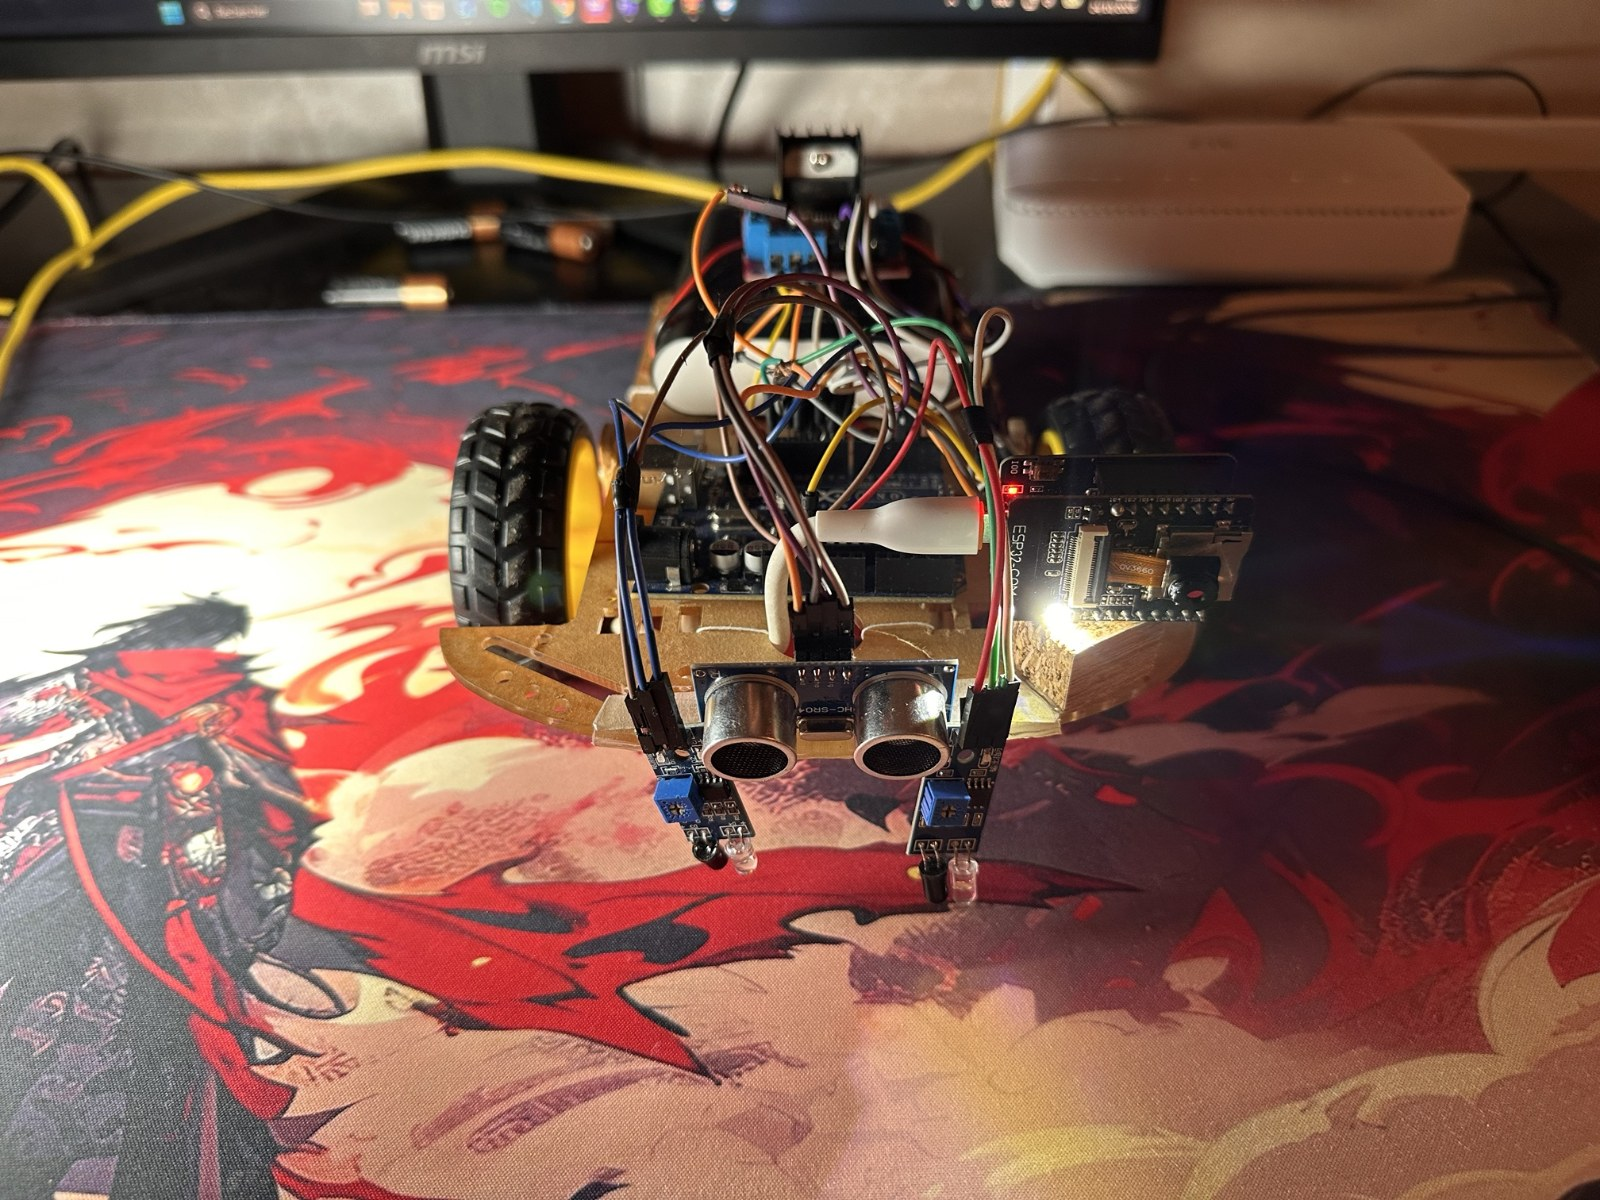
\includegraphics[height=4.6cm]{photos/prototype_avant.jpg}
  \caption{Le prototype}
\end{subfigure}\hfill
\begin{subfigure}[b]{0.31\linewidth}\centering
  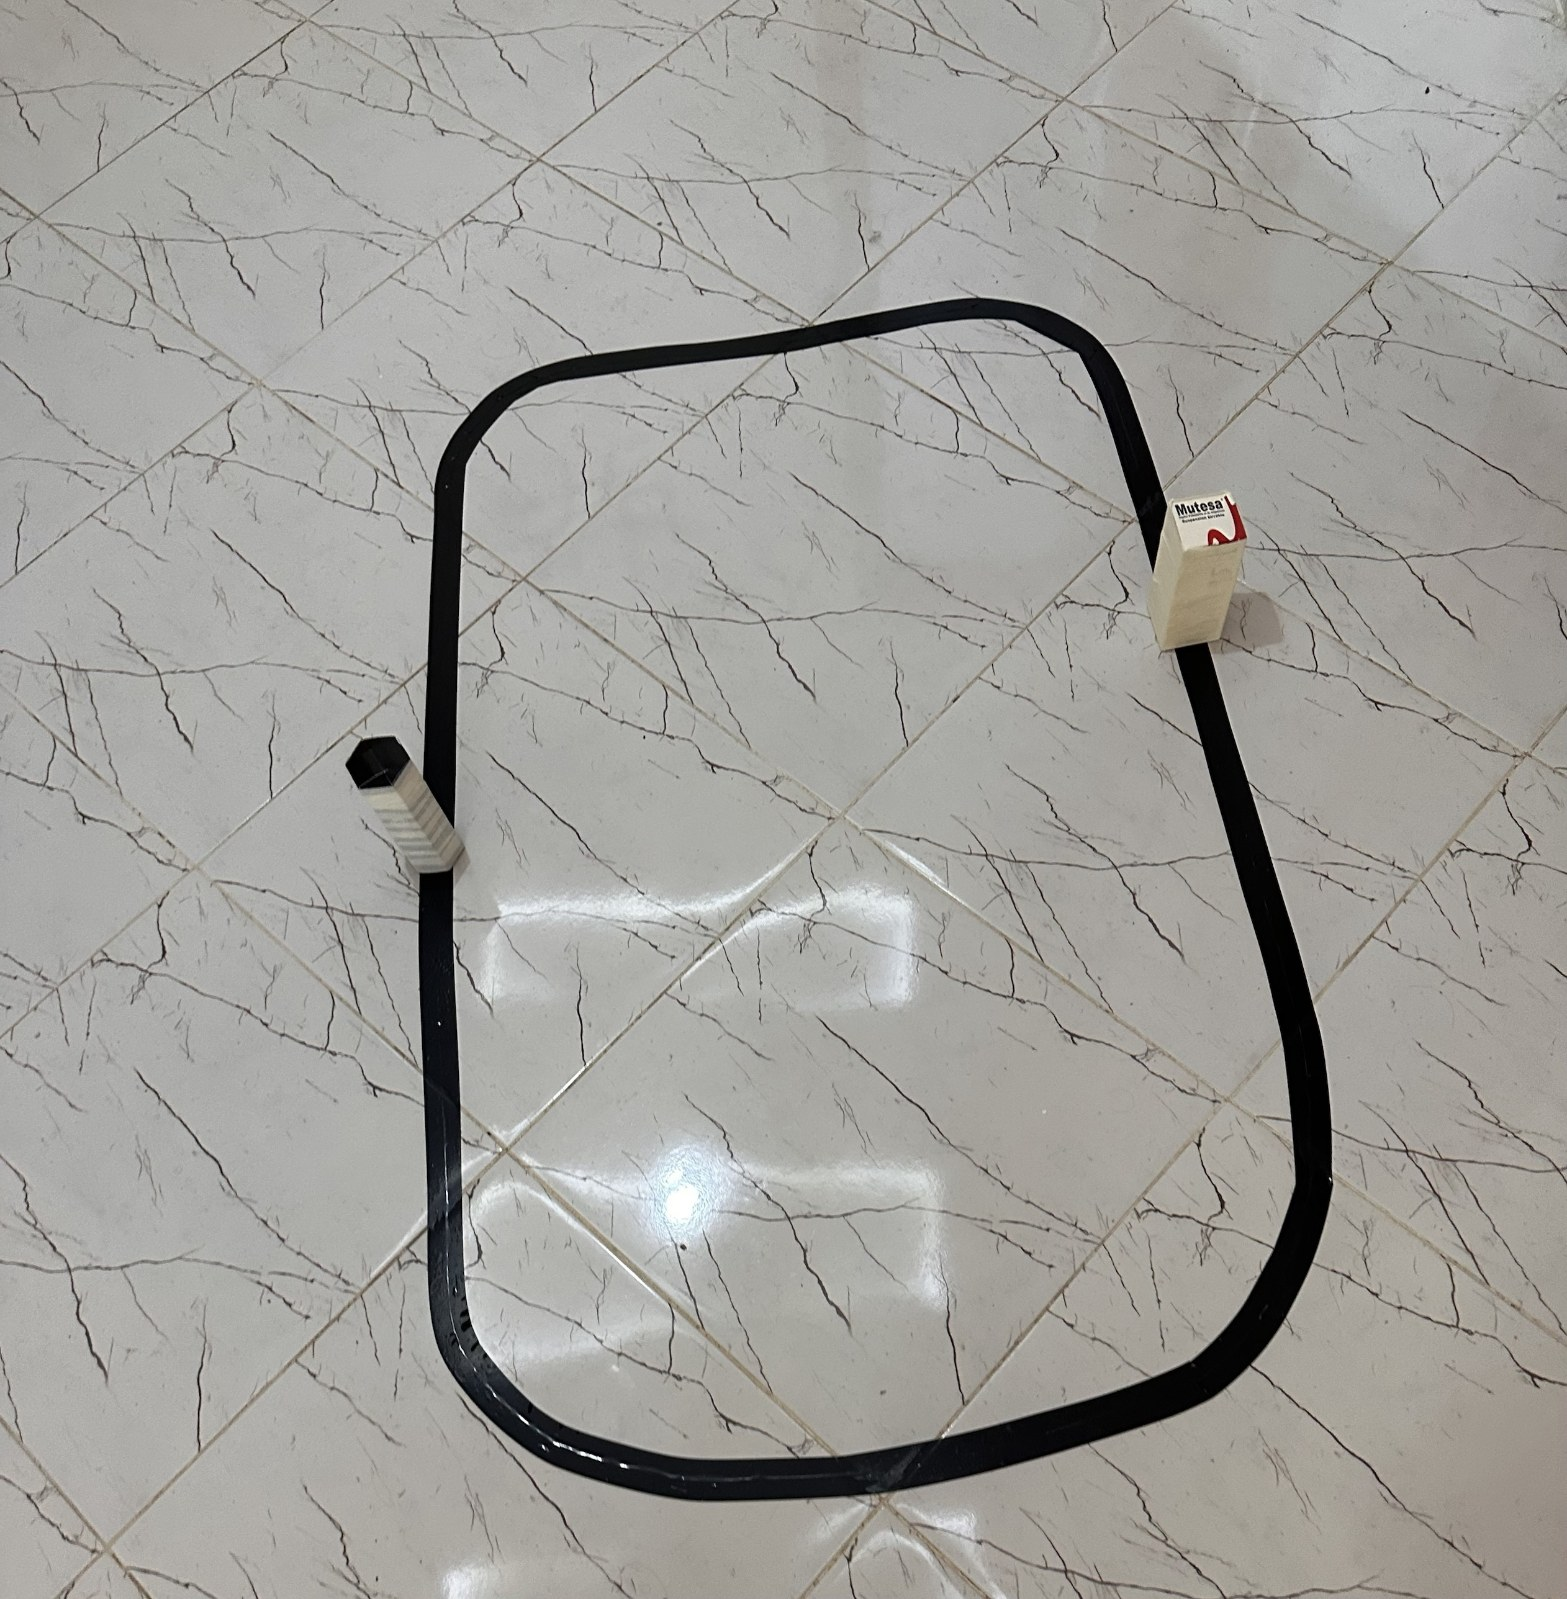
\includegraphics[height=4.6cm]{photos/piste.jpg}
  \caption{La piste et ses obstacles}
\end{subfigure}\hfill
\begin{subfigure}[b]{0.24\linewidth}\centering
  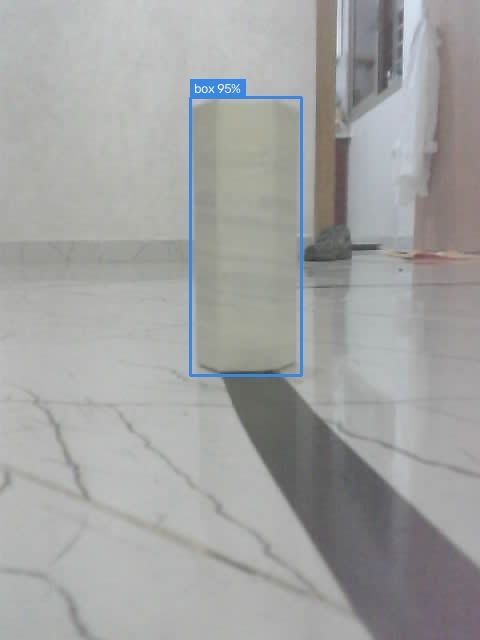
\includegraphics[height=4.6cm]{captures/esp32_detection_box.jpg}
  \caption{Vue de la caméra et détection}
\end{subfigure}

\vspace{0.3cm}
\begin{subfigure}[b]{0.49\linewidth}\centering
  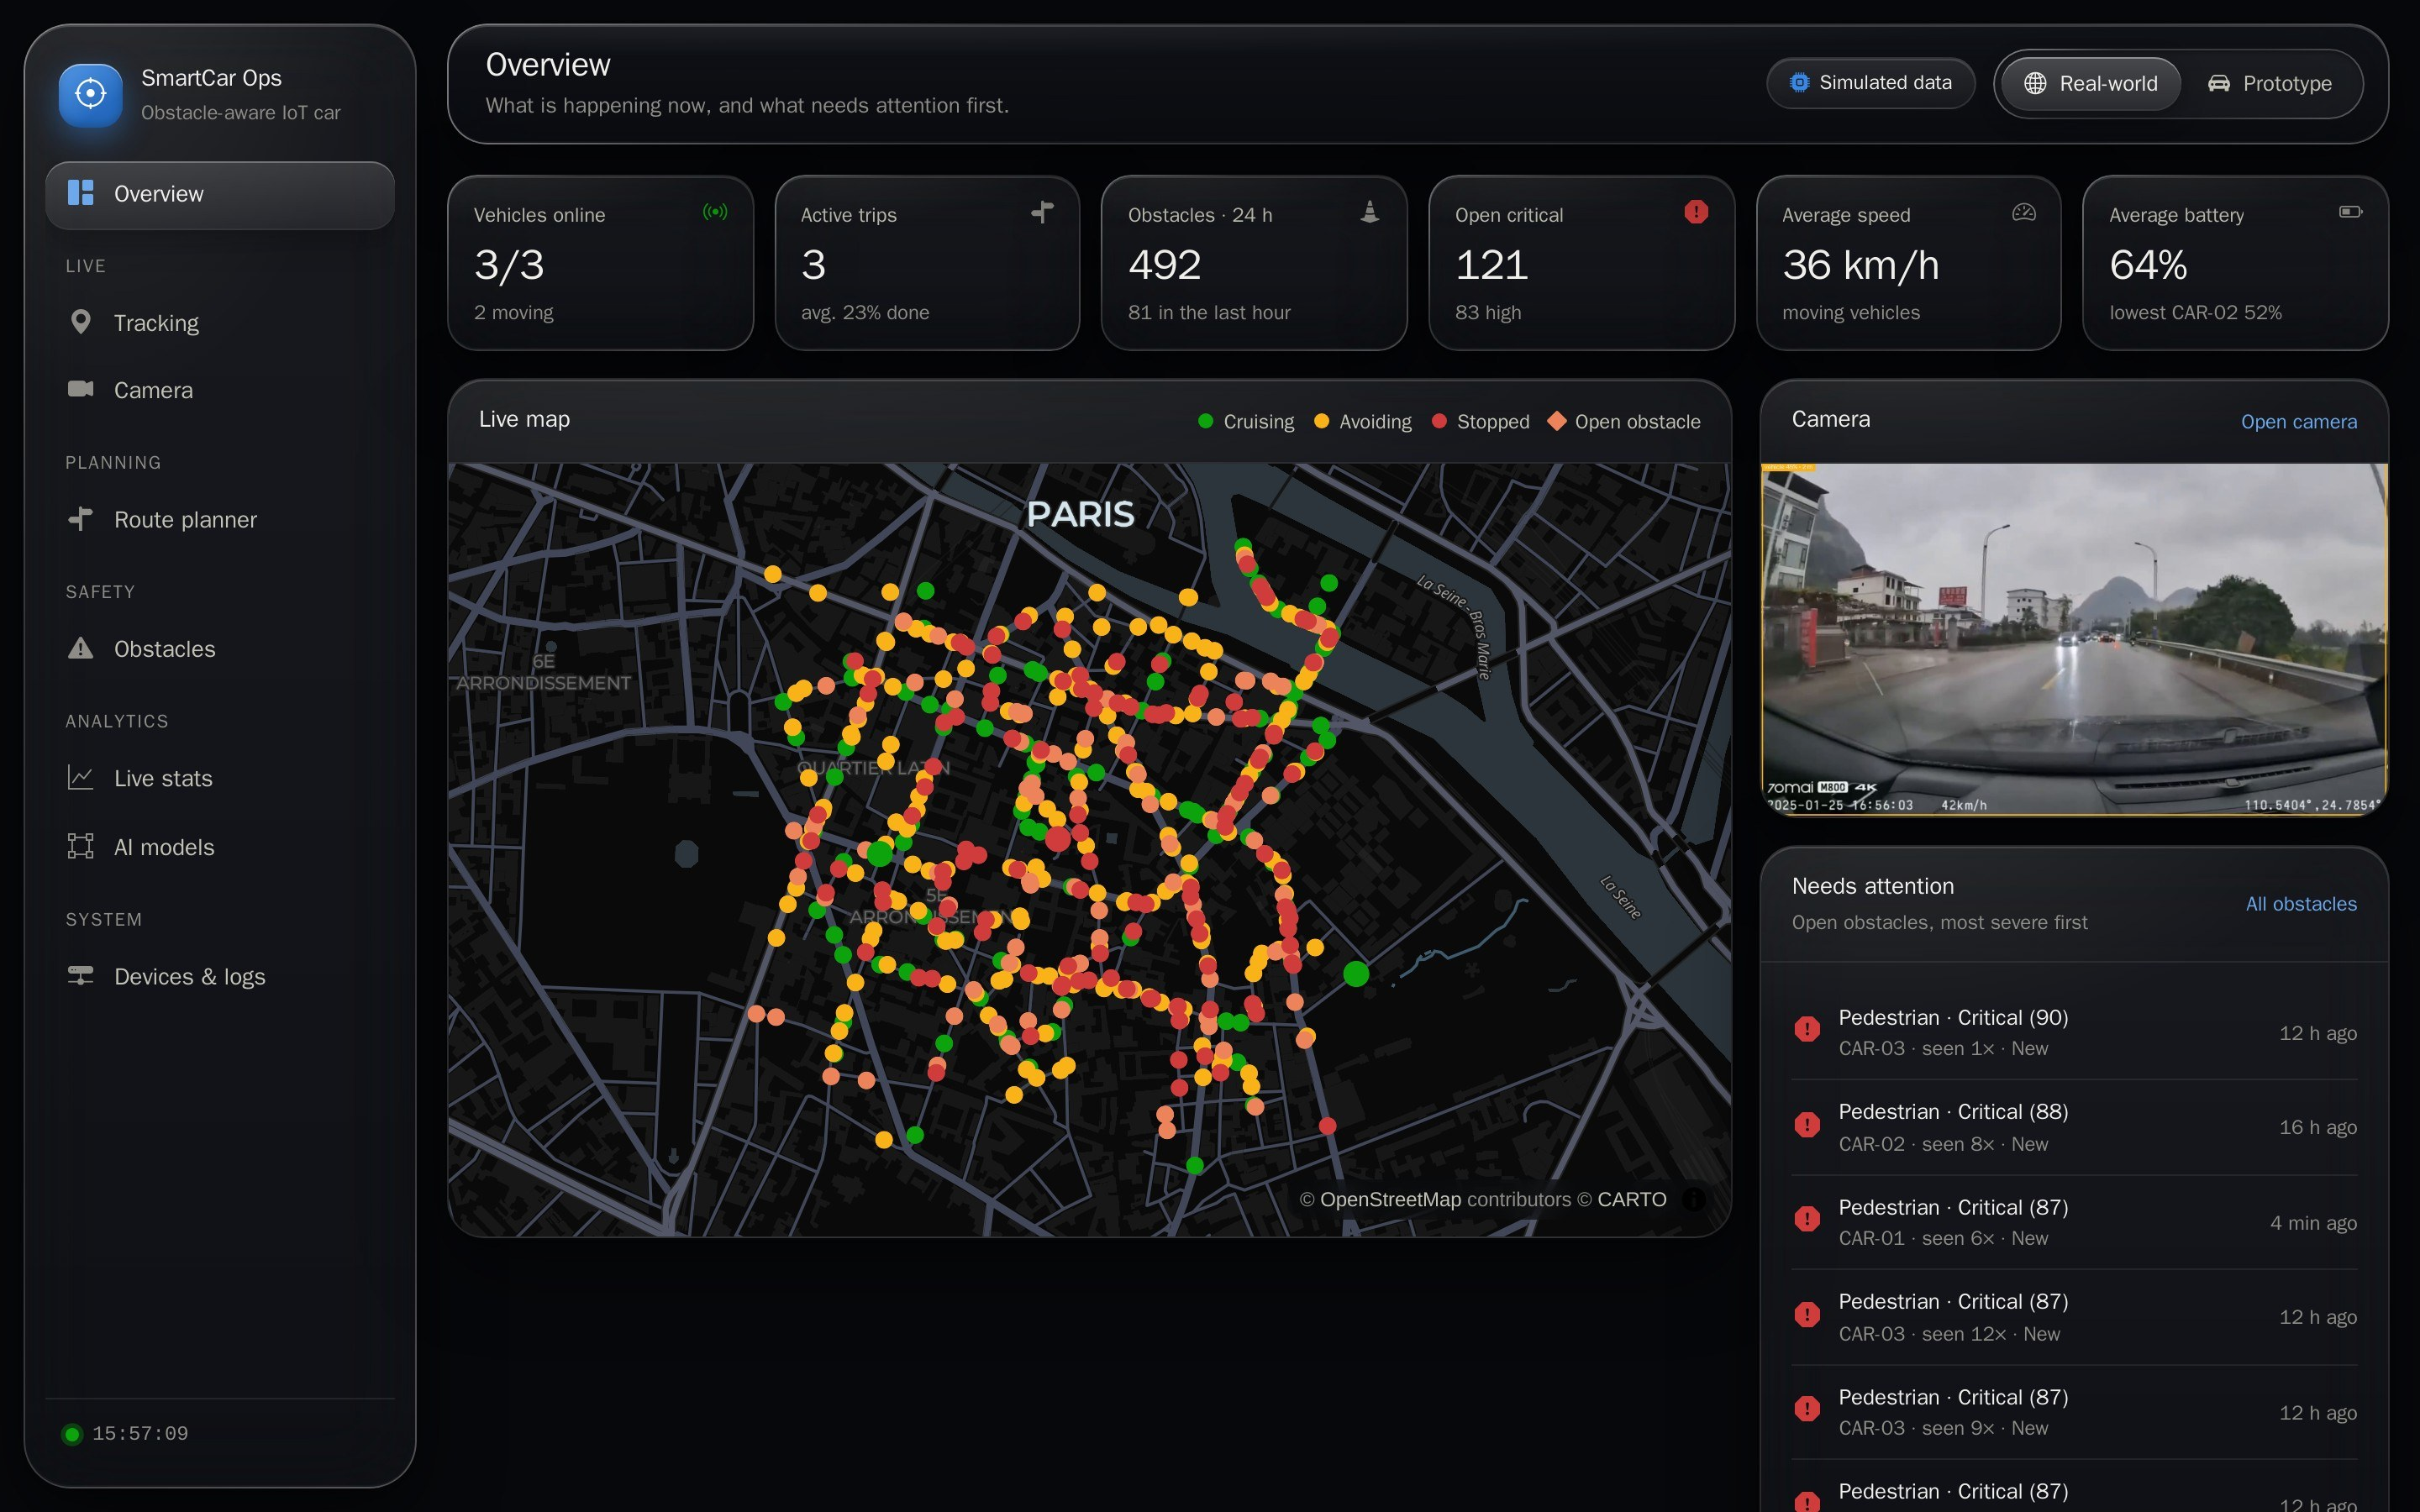
\includegraphics[width=\linewidth]{captures/overview_real_ecran.jpg}
  \caption{Environnement \emph{Monde réel}}
\end{subfigure}\hfill
\begin{subfigure}[b]{0.49\linewidth}\centering
  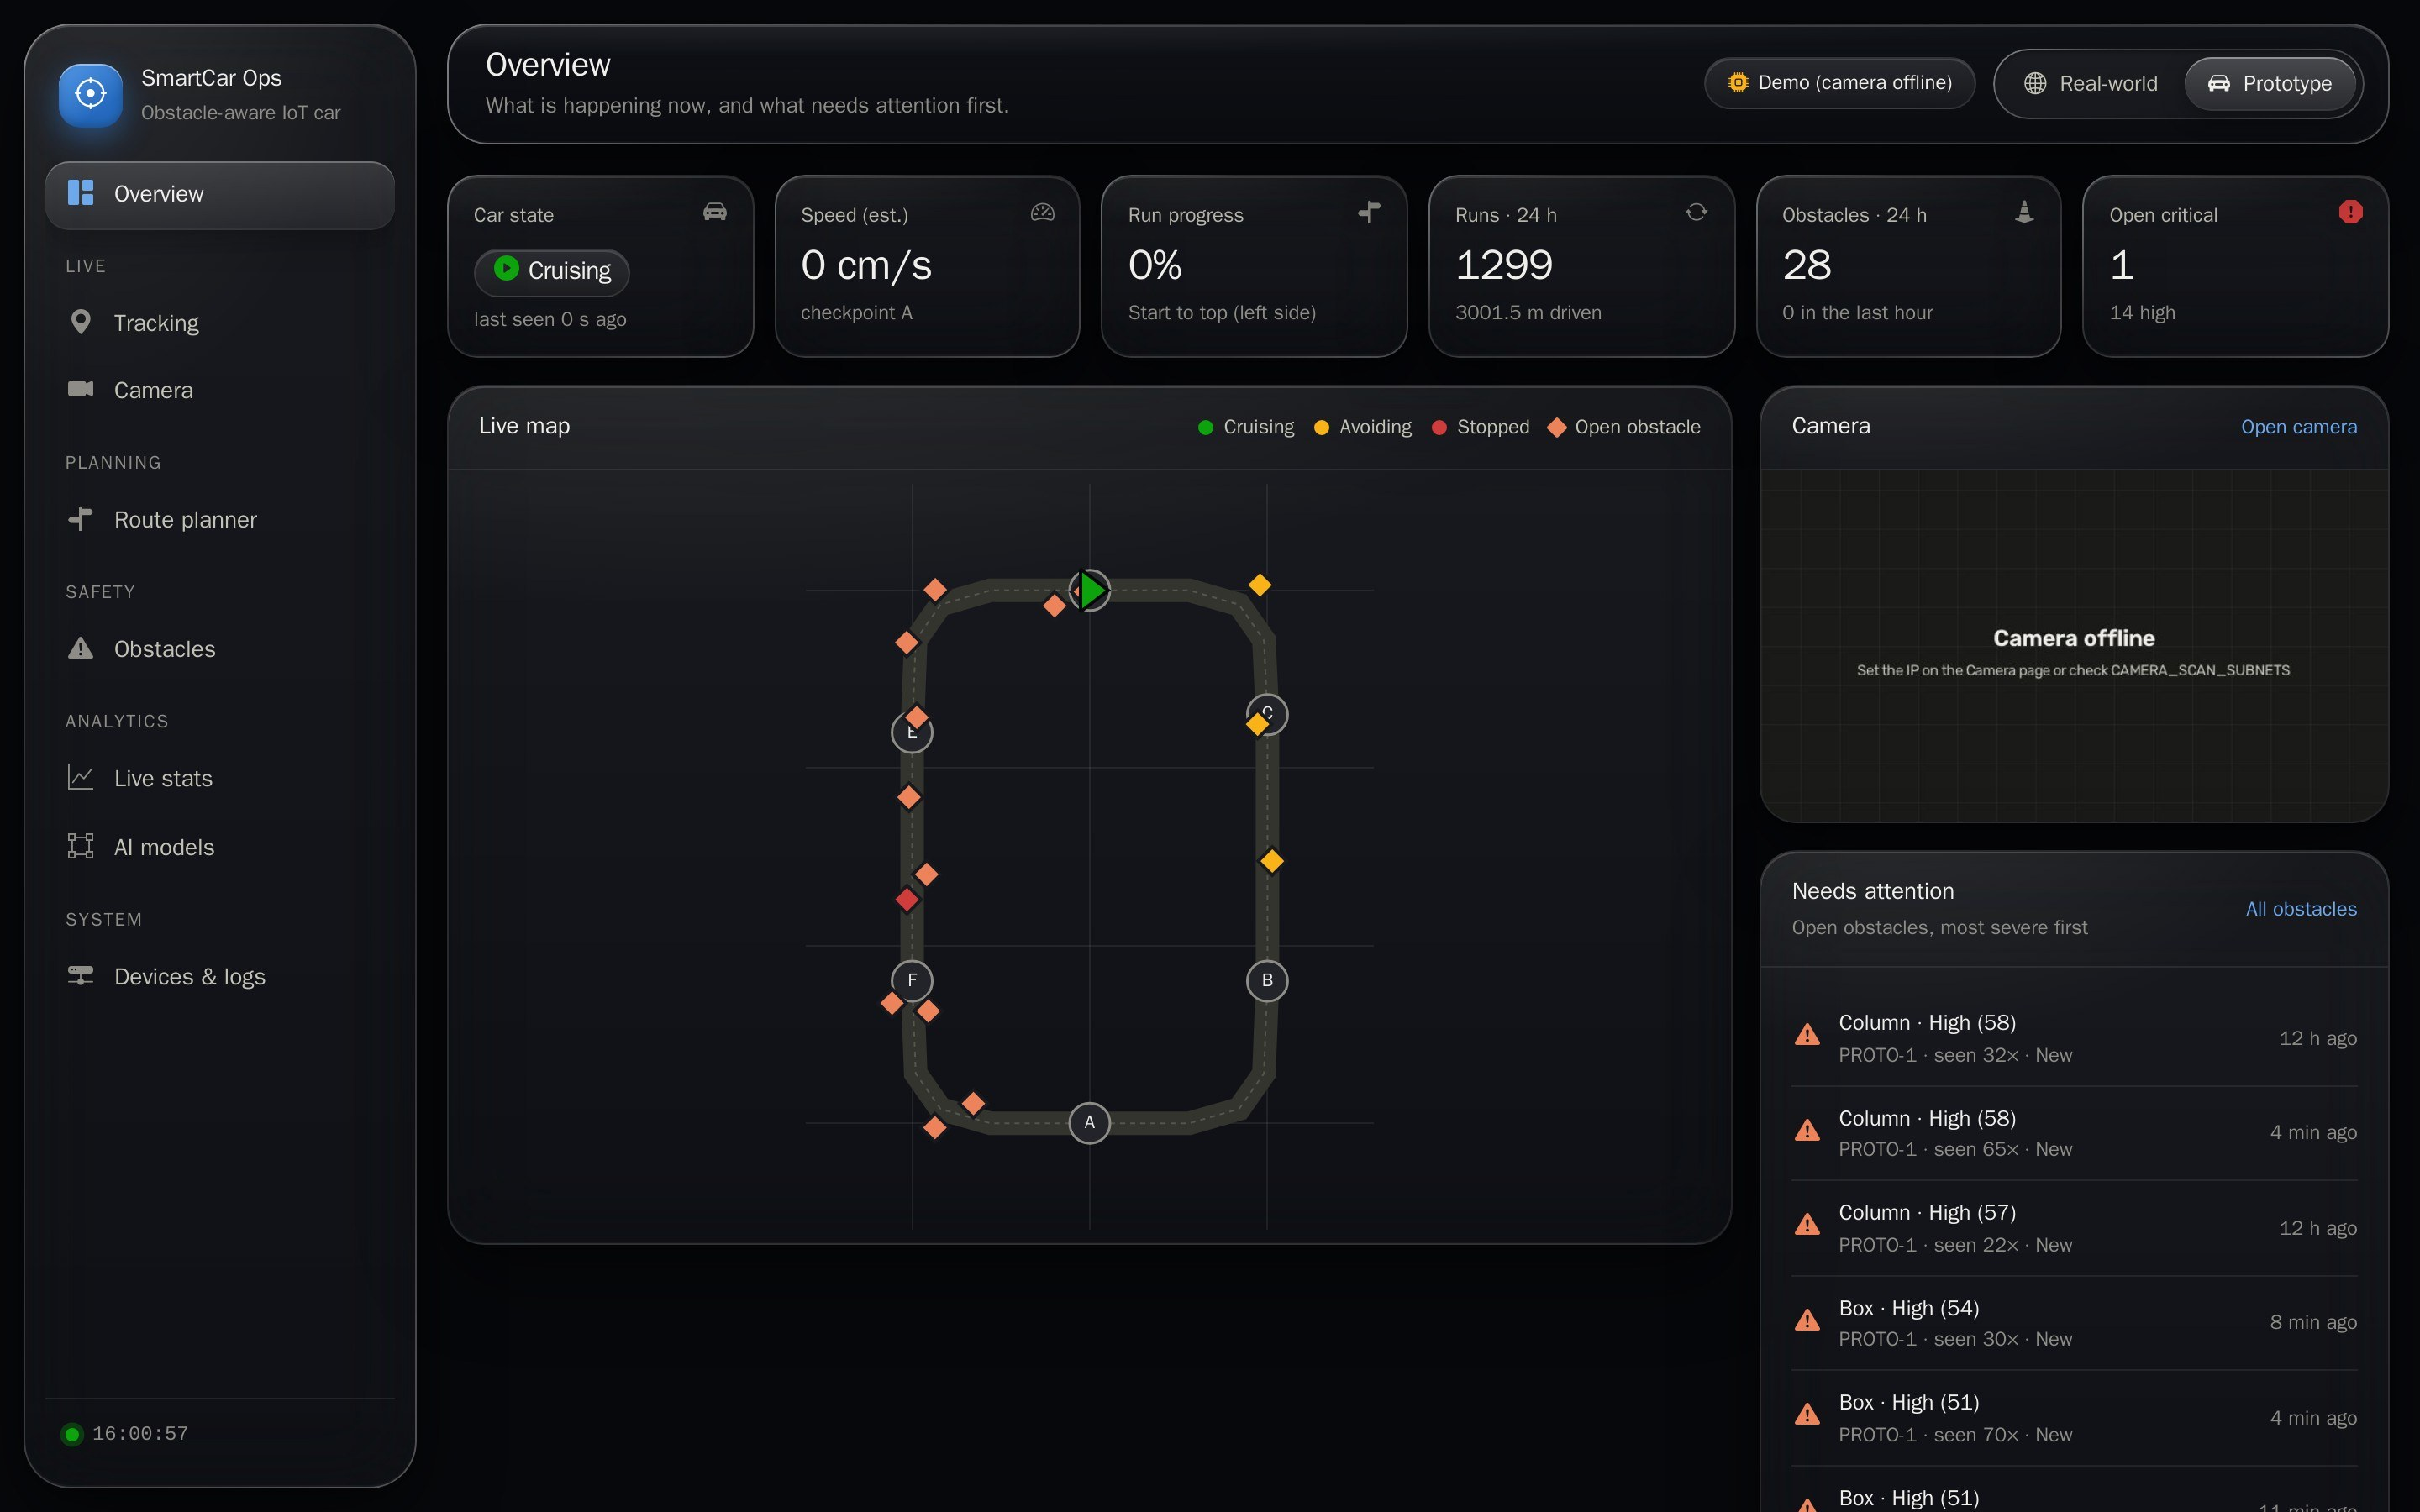
\includegraphics[width=\linewidth]{captures/overview_proto_ecran.jpg}
  \caption{Environnement \emph{Prototype}}
\end{subfigure}
\caption{Le prototype, l'application \app{} et ses deux environnements}
\label{fig:projet}
\end{figure}

% ------------------------------------------------------------------------------------------------
\section{Problématique}

La détection des obstacles routiers pose plusieurs difficultés. Les obstacles sont très variés : usagers mobiles
(piétons, cyclistes, véhicules, animaux) et anomalies statiques (nids-de-poule, cônes, barrières, panneaux de
chantier). Ils apparaissent dans des conditions changeantes de lumière, de météo et de point de vue. Les
nids-de-poule, en particulier, sont plats, de forme irrégulière et souvent peu contrastés.

Détecter ne suffit pas : un opérateur a besoin de savoir \emph{où} se trouve l'obstacle, \emph{à quel point} il
est dangereux et \emph{lequel traiter en premier}. Ces informations doivent ensuite servir à la décision, par
exemple au choix d'un itinéraire. Enfin, le prototype impose ses propres contraintes : une carte Arduino aux
ressources très limitées, une caméra peu coûteuse dont l'adresse IP change à chaque connexion, et aucune liaison
de communication entre l'Arduino et la caméra.

La problématique du projet peut donc se formuler ainsi :
\begin{center}
\begin{minipage}{0.9\linewidth}\itshape
Comment concevoir, avec des composants à faible coût, un système IoT capable de détecter automatiquement les
obstacles sur le trajet d'un véhicule, d'en évaluer la gravité et la priorité, et d'exploiter ces informations
en temps réel pour la supervision et la planification d'itinéraires, aussi bien sur des routes réelles que sur un
prototype à échelle réduite ?
\end{minipage}
\end{center}

% ------------------------------------------------------------------------------------------------
\section{Objectifs du projet}

Les objectifs fixés sont les suivants :
\begin{enumerate}
  \item \textbf{Réaliser le prototype} : assembler et câbler une voiture miniature capable de suivre une piste et
        de réagir à un obstacle, équipée d'une caméra Wi-Fi.
  \item \textbf{Entraîner des modèles de détection} : choisir des jeux de données réels d'obstacles routiers,
        entraîner un détecteur dans un environnement reproductible (notebook Jupyter dans un conteneur Docker), puis
        constituer et annoter un jeu de données propre à notre piste pour entraîner le modèle du prototype.
  \item \textbf{Évaluer honnêtement les modèles} : mesurer la précision, le rappel, le score F1, le mAP et le
        temps d'inférence sur des données jamais vues pendant l'entraînement.
  \item \textbf{Exploiter les détections} : estimer la distance et la gravité des obstacles, leur attribuer une
        priorité, les localiser et les fusionner lorsqu'ils sont vus plusieurs fois.
  \item \textbf{Développer l'application \app} : suivi des véhicules, flux vidéo annoté, planification
        d'itinéraires tenant compte des obstacles, gestion des anomalies, statistiques, présentation des modèles,
        surveillance des périphériques et des journaux, pour les deux environnements.
  \item \textbf{Assurer un déploiement simple} : l'ensemble du logiciel doit se lancer avec Docker, sans
        installation manuelle de bibliothèques.
\end{enumerate}

% ------------------------------------------------------------------------------------------------
\section{Cahier des charges}

\subsection*{Besoins fonctionnels}
\begin{itemize}
  \item \textbf{BF1 — Deux environnements} : basculer à tout moment entre \emph{Monde réel} et \emph{Prototype} ;
        chaque page s'adapte (unités en mètres ou en centimètres, carte routière ou plan de la piste).
  \item \textbf{BF2 — Vue d'ensemble} : indicateurs clés, carte en direct, obstacles à traiter, derniers
        événements.
  \item \textbf{BF3 — Suivi} : position des véhicules en temps réel, traces, état, historique des trajets et
        relecture d'un trajet passé.
  \item \textbf{BF4 — Caméra} : afficher le flux de l'ESP32-CAM malgré une adresse IP dynamique (découverte
        automatique), ou les vidéos de la caméra embarquée, avec les détections superposées.
  \item \textbf{BF5 — Planification} : choisir un départ et une destination, proposer l'itinéraire le plus court,
        le plus sûr et un compromis réglable ; éditer la piste du prototype et ses trajectoires.
  \item \textbf{BF6 — Obstacles} : liste triée par priorité, filtres, détail avec instantané, carte, actions
        (acquitter, résoudre, marquer comme faux positif).
  \item \textbf{BF7 — Statistiques} : répartitions par classe, par gravité, par heure, états des véhicules.
  \item \textbf{BF8 — Modèles d'IA} : métriques d'évaluation, matrice de confusion, comportement sur la route.
  \item \textbf{BF9 — Périphériques et journaux} : état des équipements, journal des événements, réglages
        (poids de danger des classes, données de démonstration).
\end{itemize}

\subsection*{Besoins non fonctionnels}
\begin{itemize}
  \item \textbf{Temps réel} : rafraîchissement des données chaque seconde ; analyse vidéo sur processeur sans
        bloquer l'affichage (seule l'image la plus récente est analysée).
  \item \textbf{Fiabilité} : reconnexion automatique de la caméra, base de données robuste (SQLite en mode WAL dans
        un volume Docker).
  \item \textbf{Ergonomie} : interface claire et cohérente, couleurs de gravité toujours accompagnées d'une icône et
        d'un libellé.
  \item \textbf{Portabilité et reproductibilité} : application et entraînement conteneurisés (Docker).
  \item \textbf{Évolutivité} : détecteur interchangeable (profils de modèles ONNX), configuration par variables
        d'environnement.
  \item \textbf{Honnêteté des mesures} : métriques calculées sur des ensembles de test séparés, avec le réglage
        utilisé clairement indiqué.
\end{itemize}

\subsection*{Diagramme de cas d'utilisation}
Le diagramme de la figure~\ref{fig:usecase} résume les interactions entre les acteurs et le système. L'opérateur
supervise les véhicules et les obstacles ; l'administrateur, qui est un opérateur avec des droits de
configuration, règle la caméra, la piste et les poids de danger. La caméra ESP32-CAM et la caméra embarquée du
monde réel sont des acteurs secondaires qui fournissent les images.

\begin{figure}[H]
\centering
\resizebox{\linewidth}{!}{%
\begin{tikzpicture}[
  uc/.style={ellipse,draw=bleufst,thick,fill=bleufst!7,minimum width=5.0cm,minimum height=1.05cm,align=center,
             font=\footnotesize,inner sep=0pt},
  ucs/.style={uc,draw=orangefst,fill=orangefst!10},
  lien/.style={thick,draw=encre!80},
  inc/.style={-{Stealth[length=2mm]},dashed,draw=gris,thick},
  st/.style={font=\scriptsize\itshape,text=gris,fill=white,inner sep=1pt},
  pics/acteur/.style={code={
     \draw[very thick,encre] (0,0.62) circle (0.2);
     \draw[very thick,encre] (0,0.42) -- (0,-0.12) (-0.34,0.24) -- (0.34,0.24) (0,-0.12) -- (-0.26,-0.6)
                             (0,-0.12) -- (0.26,-0.6);}}]
  % frontière du système
  \draw[thick,rounded corners=6pt,fill=fond] (-5.6,-7.3) rectangle (5.9,7.6);
  \node[font=\bfseries] at (0.15,7.2) {Système \app};
  % cas d'utilisation de l'opérateur
  \foreach \i/\t in {1/{Changer d'environnement\\(Monde réel / Prototype)},2/Consulter la vue d'ensemble,
                     3/{Suivre les véhicules\\et rejouer un trajet},4/{Visualiser le flux vidéo\\et les détections},
                     5/Planifier un itinéraire,6/{Gérer les obstacles (acquitter,\\résoudre, faux positif)},
                     7/Consulter les statistiques,8/Consulter les modèles d'IA,
                     9/{Surveiller les périphériques\\et les journaux}}
     \node[uc] (u\i) at (-2.75,7.95-1.6*\i) {\t};
  % cas internes et cas de l'administrateur
  \node[ucs] (r1) at (3.1,5.8)  {Acquérir les images\\(flux MJPEG / vidéo)};
  \node[ucs] (r2) at (3.1,3.9)  {Détecter les obstacles\\(YOLO26)};
  \node[ucs] (r3) at (3.1,1.9)  {Estimer distance,\\gravité et priorité};
  \node[ucs] (r4) at (3.1,-0.1) {Calculer le risque\\des segments};
  \node[uc]  (a1) at (3.1,-2.6) {Configurer la caméra\\(IP, rotation, enregistrement)};
  \node[uc]  (a2) at (3.1,-4.3) {Éditer la piste\\et les trajectoires};
  \node[uc]  (a3) at (3.1,-6.0) {Régler les poids\\de danger des classes};
  % acteurs
  \pic at (-8.2,1.7) {acteur}; \node[font=\small\bfseries] (op) at (-8.2,0.75) {Opérateur};
  \coordinate (opc) at (-7.8,1.6);
  \pic at (8.6,-4.3) {acteur}; \node[font=\small\bfseries,align=center] (ad) at (8.6,-5.35) {Administrateur};
  \coordinate (adc) at (8.2,-4.2);
  \pic at (8.6,6.3) {acteur}; \node[font=\small\bfseries,align=center] at (8.6,5.25) {ESP32-CAM};
  \pic at (8.6,3.2) {acteur}; \node[font=\small\bfseries,align=center] at (8.6,2.05) {Caméra embarquée\\CAR-01 (vidéo)};
  % associations
  \foreach \i in {1,...,9} \draw[lien] (opc) -- (u\i.west);
  \foreach \a in {a1,a2,a3} \draw[lien] (adc) -- (\a.east);
  \draw[lien] (8.2,6.2) -- (r1.east);
  \draw[lien] (8.2,3.1) -- (r1.south east);
  % inclusions
  \draw[inc] (u4.east) -- node[st,pos=0.45] {«include»} (r2.west);
  \draw[inc] (r2.north) -- node[st] {«include»} (r1.south);
  \draw[inc] (r2.south) -- node[st] {«include»} (r3.north);
  \draw[inc] (u6.east) -- node[st,pos=0.4] {«include»} (r3.south west);
  \draw[inc] (u5.east) -- node[st,pos=0.5] {«include»} (r4.west);
  \draw[inc] (r4.north) -- node[st] {«include»} (r3.south);
  % généralisation administrateur -> opérateur
  \draw[thick,-{Triangle[open,length=3mm,width=3mm]}] (8.6,-6.0) -- (8.6,-8.0) -- (-8.2,-8.0) -- (-8.2,0.45);
\end{tikzpicture}}
\caption{Diagramme UML de cas d'utilisation de \app}
\label{fig:usecase}
\end{figure}

% ------------------------------------------------------------------------------------------------
\section{Architecture générale du système}

La figure~\ref{fig:architecture} présente l'architecture globale, organisée selon les couches de l'IoT.

\begin{itemize}
  \item \textbf{Perception.} Dans le prototype, l'Arduino UNO lit les deux capteurs infrarouges et le capteur
        ultrasonique, et pilote les deux moteurs à travers le L298N : c'est la boucle de commande embarquée, autonome.
        L'ESP32-CAM, alimentée séparément, filme la piste. Dans le monde réel, la perception est assurée par des
        vidéos de caméras embarquées et par un simulateur de flotte qui produit la télémétrie des véhicules.
  \item \textbf{Réseau.} L'ESP32-CAM diffuse un flux MJPEG en HTTP sur le réseau Wi-Fi local (port 81) et expose une
        interface de réglage (port 80). Son adresse IP étant attribuée dynamiquement, le serveur la retrouve par
        balayage du sous-réseau.
  \item \textbf{Traitement.} Un conteneur Docker héberge le serveur : relais du flux vidéo (la caméra n'accepte
        qu'un seul client), redressement de l'image, détection d'objets par les modèles YOLO26 exportés en ONNX,
        lecture des marqueurs ArUco, estimation de la distance, de la gravité et de la priorité, fusion des
        détections répétées, calcul du risque des segments et planification d'itinéraires. Les données sont
        stockées dans une base SQLite. Un second conteneur, utilisé hors ligne, sert à l'entraînement des modèles
        sur GPU (JupyterLab et Ultralytics).
  \item \textbf{Application.} L'application Dash présente les huit pages de supervision dans le navigateur de
        l'opérateur et se rafraîchit chaque seconde.
\end{itemize}

\begin{figure}[H]
\centering
\resizebox{\linewidth}{!}{%
% Architecture globale du système (figure du chapitre 1)
\begin{tikzpicture}[
  b/.style={bloc,font=\footnotesize,minimum width=3cm,text width=2.8cm,minimum height=1cm},
  bo/.style={b,draw=orangefst,fill=orangefst!12},
  bv/.style={b,draw=vertfst!80!black,fill=vertfst!15},
  bg/.style={b,fill=bleufst!10}]
  % ---- perception : prototype
  \node[bo] (sens) at (1.7,-0.75) {Capteurs IR\\+ HC-SR04};
  \node[bo] (uno)  at (1.7,-2.15) {Arduino UNO\\(commande)};
  \node[bo] (mot)  at (1.7,-3.55) {L298N\\+ 2 moteurs DC};
  \node[bo] (cam)  at (5.1,-2.15) {ESP32-CAM\\(OV3660)};
  \draw[fleche] (sens) -- (uno); \draw[fleche] (uno) -- (mot);
  \begin{scope}[on background layer]
    \node[zone,fill=orangefst!5,fit=(sens)(mot)(cam),
          label={[font=\bfseries\small]above:Prototype — perception}] (zp) {};
  \end{scope}
  % ---- perception : monde réel
  \node[bv] (vid) at (8.5,-2.15)  {Vidéos de route\\(dashcam de CAR-01)};
  \node[bv] (sim) at (12.0,-2.15) {Simulateur de flotte\\(3 véhicules)};
  \node[bv] (osm) at (15.5,-2.15) {Graphe routier OSM\\(Quartier Latin)};
  \begin{scope}[on background layer]
    \node[zone,fill=vertfst!6,fit=(vid)(osm)(vid|-sens.north)(vid|-mot.south),
          label={[font=\bfseries\small]above:Monde réel — perception}] (zr) {};
  \end{scope}
  % ---- réseau
  \node[b,draw=orangefst,fill=white] (wifi) at (5.1,-5.0) {Wi-Fi 802.11\\HTTP : flux MJPEG};
  \draw[fleche] (cam) -- (wifi);
  % ---- traitement (serveur)
  \node[bg] (relay) at (1.7,-7.2)  {Découverte IP\\+ relais MJPEG};
  \node[bg] (perc)  at (5.1,-7.2)  {Perception : rotation,\\ArUco, mouvement};
  \node[bg] (onnx)  at (8.5,-7.2)  {Inférence YOLO26\\(ONNX Runtime)};
  \node[bg] (sev)   at (13.2,-7.2) {Distance, gravité,\\priorité, fusion};
  \node[bg] (db)    at (5.1,-8.9)  {SQLite (WAL)\\+ instantanés};
  \node[bg] (hub)   at (8.5,-8.9)  {Télémétrie en direct\\(hub mémoire)};
  \node[bg] (plan)  at (13.2,-8.9) {Risque des segments\\+ planificateur};
  \draw[fleche] (wifi.south) -- ++(0,-0.55) -| (relay.north);
  \draw[fleche] (relay) -- (perc); \draw[fleche] (perc) -- (onnx); \draw[fleche] (onnx) -- (sev);
  \draw[fleche] (sev) -- (plan); \draw[fleche] (perc) -- (db);
  \draw[fleche] (perc.south east) -- (hub.north west);
  \draw[fleche] (vid) -- (onnx);
  \draw[fleche] ([xshift=-1.0cm]sim.south) -- ++(0,-5.3) -| ([xshift=0.6cm]hub.north);
  \draw[fleche] (osm.south) |- (plan.east);
  \begin{scope}[on background layer]
    \node[zone,fill=bleufst!5,fit=(relay)(sev)(plan)(db)(osm.east|-plan.south),
          label={[font=\bfseries\small,anchor=south east]north east:Serveur — conteneur Docker (traitement)}] (zs) {};
  \end{scope}
  % ---- application
  \node[b,minimum width=6.4cm,text width=6.2cm] (dash) at (8.5,-11.2) {\textbf{Application Dash \app}\\8 pages, rafraîchies chaque seconde};
  \node[b] (nav) at (13.7,-11.2) {Navigateur\\de l'opérateur};
  \node[b,draw=gris,fill=gris!10] (train) at (2.3,-11.2) {Entraînement (GPU)\\JupyterLab + Ultralytics};
  \draw[fleche] (zs.south -| dash.north) -- (dash);
  \draw[fleche,{Stealth[length=2.6mm]}-{Stealth[length=2.6mm]}] (dash) -- (nav);
  \draw[fleche,dashed,draw=gris] (train.north) -- (train.north |- zs.south) node[note,midway,right] {modèles ONNX};
\end{tikzpicture}
}
\caption{Architecture globale du système}
\label{fig:architecture}
\end{figure}

\chapconclusion
Ce chapitre a présenté le contexte de l'IoT et de son association avec l'intelligence artificielle, puis le projet
lui-même : un prototype, des modèles de détection et une application de supervision couvrant deux
environnements. Le cahier des charges et l'architecture générale fixent le cadre des chapitres suivants. Le
chapitre~2 détaille la réalisation matérielle du prototype.

\chapter{Conception et réalisation matérielle}

\tikzset{
  annot/.style={draw=orangefst,very thick,{Circle[length=4.5pt,fill=orangefst]}-},
  lab/.style={font=\scriptsize,fill=white,draw=orangefst!60,rounded corners=2pt,inner sep=2.5pt,align=left},
}

\section{Introduction}
Ce chapitre décrit la partie matérielle du projet : la voiture miniature qui constitue l'environnement
\emph{prototype}. Nous présentons d'abord l'architecture matérielle d'ensemble, puis chacun des composants
(rôle, caractéristiques et broches utilisées), le système d'alimentation, le schéma de câblage et enfin la
réalisation physique du prototype et de sa piste.

% ------------------------------------------------------------------------------------------------
\section{Architecture matérielle du système}

Le prototype est organisé autour de deux sous-systèmes indépendants (figure~\ref{fig:archi-materielle}) :
\begin{itemize}
  \item \textbf{le sous-système de commande}, construit autour de l'Arduino UNO, qui lit les capteurs infrarouges
        et ultrasonique et commande les deux moteurs à travers le pont en H L298N. Il assure de manière autonome
        le suivi de la piste et l'arrêt devant un obstacle ;
  \item \textbf{le sous-système de vision}, formé de l'ESP32-CAM montée sur sa carte ESP32-CAM-MB et alimentée par
        une batterie externe. Il filme la route et diffuse les images en Wi-Fi vers le serveur \app.
\end{itemize}
Les deux sous-systèmes ne sont pas reliés entre eux : il n'existe pas de liaison série entre l'Arduino et
l'ESP32-CAM. Toutes les informations du prototype affichées par l'application proviennent donc de l'image.

\begin{figure}[H]
\centering
\resizebox{\linewidth}{!}{%
\begin{tikzpicture}[node distance=0.5cm and 0.9cm,
  pw/.style={-{Stealth[length=2.4mm]},very thick,draw=critique!85},
  sg/.style={-{Stealth[length=2.4mm]},thick,draw=bleufst},
  lb/.style={font=\scriptsize,fill=white,inner sep=1pt}]
  \node[bloco,minimum width=2.6cm] (bat) {4 piles AA\\($\approx$ 6 V)};
  \node[bloco,minimum width=2.6cm,below=0.9cm of bat] (sw) {Interrupteur};
  \node[blocg,minimum width=3cm,minimum height=2.2cm,right=1.6cm of sw] (l298) {Pont en H\\L298N};
  \node[bloc,minimum width=2.6cm,above right=0.2cm and 1.2cm of l298] (mg) {Moteur gauche};
  \node[bloc,minimum width=2.6cm,below right=0.2cm and 1.2cm of l298] (md) {Moteur droit};
  \node[blocg,minimum width=3.4cm,minimum height=2.4cm,below=2.2cm of l298] (uno) {Arduino UNO\\ATmega328P};
  \node[bloc,minimum width=2.6cm,left=2.2cm of uno.north west,anchor=north east] (irg) {Capteur IR gauche};
  \node[bloc,minimum width=2.6cm,below=0.35cm of irg] (ird) {Capteur IR droit};
  \node[bloc,minimum width=2.6cm,below=0.35cm of ird] (us) {HC-SR04};
  \node[bloco,minimum width=3cm,right=1.7cm of mg] (pb) {Batterie externe\\5 V (USB)};
  \node[bloc,minimum width=3cm,below=0.9cm of pb] (mb) {ESP32-CAM-MB\\(USB / programmation)};
  \node[blocg,minimum width=3cm,below=0.5cm of mb] (cam) {ESP32-CAM\\caméra OV3660};
  \node[bloc,draw=gris,minimum width=3cm,below=1.3cm of cam] (srv) {Serveur \app\\(ordinateur portable)};
  % alimentation
  \draw[pw] (bat) -- node[lb,right] {+} (sw);
  \draw[pw] (sw) -- node[lb,above] {VS} (l298);
  \draw[pw] (pb) -- node[lb,right] {5 V} (mb);
  \draw[pw,dashed] (pb.south west) to[out=-120,in=0] node[lb,pos=0.7,below] {5 V (USB)} (uno.east);
  \draw[pw] (mb) -- (cam);
  \draw[pw,{Stealth[length=2.4mm]}-{Stealth[length=2.4mm]}] (l298.south) -- node[lb,right] {5 V / GND communs} (uno.north);
  % moteurs
  \draw[sg,draw=encre] (l298.east) ++(0,0.4) -- node[lb,above,sloped] {OUT1--OUT2} (mg.west);
  \draw[sg,draw=encre] (l298.east) ++(0,-0.4) -- node[lb,below,sloped] {OUT3--OUT4} (md.west);
  % signaux
  \draw[sg] (irg.east) -- node[lb,above] {D2} (irg.east -| uno.west);
  \draw[sg] (ird.east) -- node[lb,above] {D3} (ird.east -| uno.west);
  \draw[sg,{Stealth[length=2.4mm]}-{Stealth[length=2.4mm]}] (us.east) -- node[lb,above] {D12 Trig / D13 Echo} (us.east -| uno.west);
  \draw[sg] ([xshift=0.8cm]uno.north) -- node[lb,right] {D8--D11 $\rightarrow$ IN1--IN4} ([xshift=0.8cm]l298.south);
  % wifi
  \draw[sg,dashed,draw=vertfst!70!black] (cam) -- node[lb,right] {Wi-Fi : flux MJPEG} (srv);
  \begin{scope}[on background layer]
    \node[zone,fill=bleufst!4,fit=(bat)(l298)(mg)(md)(uno)(irg)(us),label={[font=\bfseries\small]above:Sous-système de commande}] {};
    \node[zone,fill=vertfst!5,fit=(pb)(mb)(cam),label={[font=\bfseries\small]above:Sous-système de vision}] {};
  \end{scope}
  \node[font=\scriptsize,align=left,anchor=north west] at ($(us.south west)+(0,-0.5)$)
    {\textcolor{critique}{\rule[2pt]{0.6cm}{1.4pt}} alimentation \quad \textcolor{bleufst}{\rule[2pt]{0.6cm}{1.2pt}} signaux
     \quad \textcolor{vertfst!70!black}{- - -} liaison sans fil};
\end{tikzpicture}}
\caption{Architecture matérielle du prototype}
\label{fig:archi-materielle}
\end{figure}

Le tableau~\ref{tab:composants} récapitule les composants utilisés.

\begin{table}[H]
\centering\small
\caption{Composants du prototype}
\label{tab:composants}
\begin{tabularx}{\linewidth}{l c X}
\toprule
\textbf{Composant} & \textbf{Qté} & \textbf{Rôle} \\
\midrule
Arduino UNO (ATmega328P)          & 1 & Unité de commande : lecture des capteurs, commande des moteurs \\
Module L298N (double pont en H)   & 1 & Interface de puissance entre l'Arduino et les moteurs \\
Moteur à courant continu avec réducteur (« TT ») & 2 & Propulsion et direction différentielle \\
Capteur infrarouge à réflexion    & 2 & Détection du ruban noir de la piste (gauche / droite) \\
Capteur ultrasonique HC-SR04      & 1 & Mesure de la distance à l'obstacle frontal \\
ESP32-CAM + carte ESP32-CAM-MB    & 1 & Acquisition et diffusion Wi-Fi des images \\
4 piles alcalines AA 1,5 V + interrupteur & 1 & Alimentation des moteurs \\
Batterie externe USB 5 V          & 1 & Alimentation de la caméra et de l'électronique de commande \\
Châssis, roues, roue folle, fils Dupont & — & Structure mécanique et liaisons \\
\bottomrule
\end{tabularx}
\end{table}

% ------------------------------------------------------------------------------------------------
\section{Arduino UNO}

L'Arduino UNO est une carte de développement construite autour du microcontrôleur 8 bits ATmega328P de
Microchip~\cite{arduinouno}. Elle est simple à programmer (langage Arduino, dérivé du C++), robuste et bien
documentée, ce qui en fait un choix naturel pour la boucle de commande du prototype. Ses principales
caractéristiques sont données dans le tableau~\ref{tab:uno}, et la figure~\ref{fig:uno} identifie ses broches
principales.

\begin{table}[H]
\centering\small
\caption{Caractéristiques principales de l'Arduino UNO}
\label{tab:uno}
\begin{tabular}{ll}
\toprule
Microcontrôleur & ATmega328P, 8 bits, 16 MHz \\
Mémoires & 32 Ko de Flash, 2 Ko de SRAM, 1 Ko d'EEPROM \\
Entrées / sorties numériques & 14 (dont 6 compatibles MLI/PWM) \\
Entrées analogiques & 6 (A0 à A5), convertisseur 10 bits \\
Tension de fonctionnement & 5 V (alimentation par USB ou prise jack 7--12 V) \\
Courant maximal par broche & 20 mA recommandés (40 mA absolus) \\
\bottomrule
\end{tabular}
\end{table}

\begin{figure}[H]
\centering
\begin{tikzpicture}
  \node[anchor=south west,inner sep=0] (img) at (0,0) {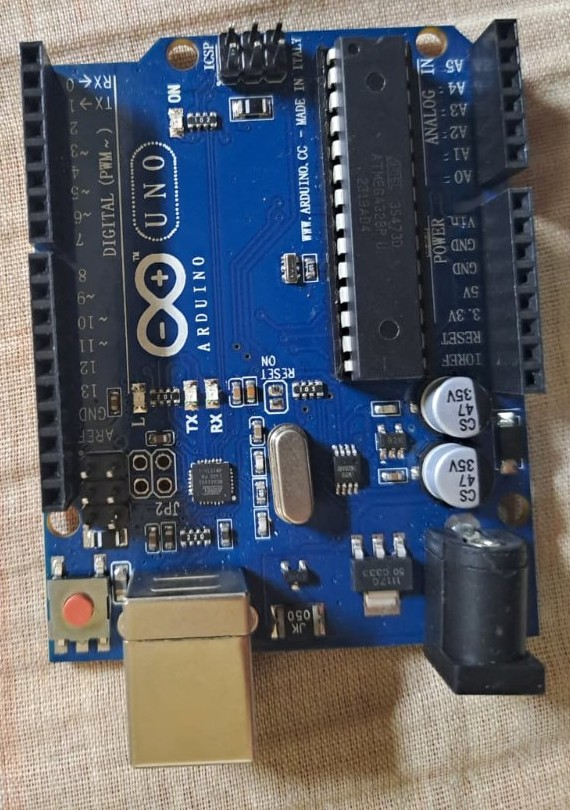
\includegraphics[width=5.4cm]{photos/arduino_uno_crop.jpg}};
  \begin{scope}[x={(img.south east)},y={(img.north west)}]
    \draw[annot] (0.06,0.83) -- (-0.12,0.83) node[lab,left] {Broches numériques D0--D7\\(D2, D3 : capteurs IR)};
    \draw[annot] (0.06,0.57) -- (-0.12,0.57) node[lab,left] {Broches D8--D13\\(D8--D11 : L298N ; D12, D13 : HC-SR04)};
    \draw[annot] (0.135,0.247) -- (-0.12,0.30) node[lab,left] {Bouton de réinitialisation};
    \draw[annot] (0.325,0.13) -- (-0.12,0.08) node[lab,left] {Port USB-B\\(programmation, alimentation)};
    \draw[annot] (0.447,0.93) -- (1.12,0.97) node[lab,right] {Connecteur ICSP};
    \draw[annot] (0.66,0.74) -- (1.12,0.78) node[lab,right] {Microcontrôleur\\ATmega328P};
    \draw[annot] (0.895,0.877) -- (1.12,0.88) node[lab,right] {Entrées analogiques A0--A5};
    \draw[annot] (0.91,0.654) -- (1.12,0.60) node[lab,right] {Alimentation :\\5 V, 3,3 V, GND, Vin};
    \draw[annot] (0.51,0.42) -- (1.12,0.42) node[lab,right] {Quartz 16 MHz};
    \draw[annot] (0.85,0.235) -- (1.12,0.22) node[lab,right] {Prise jack (7--12 V)};
  \end{scope}
\end{tikzpicture}
\caption{Carte Arduino UNO du prototype et ses broches principales}
\label{fig:uno}
\end{figure}

Dans notre montage, l'Arduino utilise huit broches numériques (tableau~\ref{tab:broches}). Les broches D2 et D3
reçoivent les sorties tout-ou-rien des capteurs infrarouges ; D8 à D11 imposent le sens de rotation des moteurs
au L298N ; D12 déclenche la mesure du HC-SR04 et D13 en reçoit l'écho.

\begin{table}[H]
\centering\small
\caption{Affectation des broches de l'Arduino UNO}
\label{tab:broches}
\begin{tabular}{lll}
\toprule
\textbf{Broche} & \textbf{Connectée à} & \textbf{Rôle} \\
\midrule
D2  & Capteur IR gauche (OUT) & Entrée : ruban détecté à gauche \\
D3  & Capteur IR droit (OUT)  & Entrée : ruban détecté à droite \\
D8, D9 & L298N IN1, IN2 & Sorties : sens du moteur gauche \\
D10, D11 & L298N IN3, IN4 & Sorties : sens du moteur droit \\
D12 & HC-SR04 Trig & Sortie : impulsion de déclenchement (10 µs) \\
D13 & HC-SR04 Echo & Entrée : durée de l'écho \\
5 V, GND & L298N, HC-SR04, capteurs IR & Alimentation logique et masse commune \\
\bottomrule
\end{tabular}
\end{table}

% ------------------------------------------------------------------------------------------------
\section{Module L298N}

Un microcontrôleur ne peut fournir que quelques dizaines de milliampères par broche, alors qu'un moteur en
consomme plusieurs centaines. Le module L298N sert d'interface de puissance : il contient deux ponts en H qui
permettent de commander indépendamment le sens (et, par les entrées ENA/ENB, la vitesse) de deux moteurs à courant
continu~\cite{l298}. Il accepte une tension moteur de 5 à 35 V, un courant de 2 A par voie, et intègre un
régulateur 5 V (78M05). Les bornes et entrées du module sont identifiées sur la figure~\ref{fig:l298n}.

\begin{figure}[H]
\centering
\begin{tikzpicture}
  \node[anchor=south west,inner sep=0] (img) at (0,0) {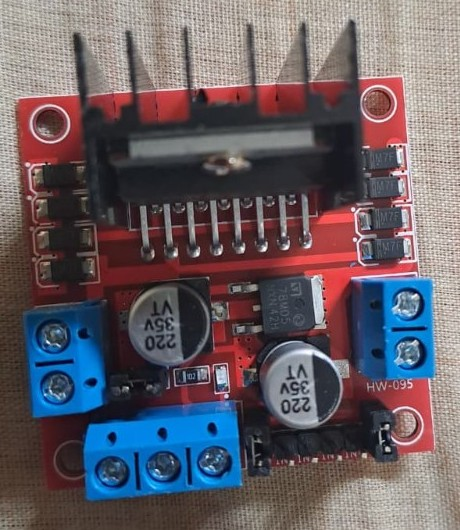
\includegraphics[width=6cm]{photos/l298n_crop.jpg}};
  \begin{scope}[x={(img.south east)},y={(img.north west)}]
    \draw[annot] (0.478,0.736) -- (1.1,0.86) node[lab,right] {Circuit L298N\\et son radiateur};
    \draw[annot] (0.63,0.415) -- (1.1,0.66) node[lab,right] {Régulateur 5 V (78M05)};
    \draw[annot] (0.859,0.377) -- (1.1,0.45) node[lab,right] {Sortie moteur B\\(OUT3, OUT4) $\rightarrow$ moteur droit};
    \draw[annot] (0.696,0.155) -- (1.1,0.16) node[lab,right] {Entrées IN1--IN4\\et cavaliers ENA / ENB};
    \draw[annot] (0.141,0.32) -- (-0.1,0.48) node[lab,left] {Sortie moteur A\\(OUT1, OUT2) $\rightarrow$ moteur gauche};
    \draw[annot] (0.289,0.274) -- (-0.1,0.28) node[lab,left] {Cavalier d'activation\\du régulateur 5 V};
    \draw[annot] (0.352,0.132) -- (-0.1,0.08) node[lab,left] {Bornier d'alimentation :\\VS (+6 V), GND, +5 V};
  \end{scope}
\end{tikzpicture}
\caption{Module L298N : bornes d'alimentation, entrées de commande et sorties moteurs}
\label{fig:l298n}
\end{figure}

Les cavaliers ENA et ENB étant en place, les deux moteurs tournent à pleine tension et leur sens est fixé par les
entrées IN (tableau~\ref{tab:l298}). La direction de la voiture est obtenue par \emph{commande différentielle} :
pour tourner à gauche, on ralentit ou on arrête le moteur gauche pendant que le moteur droit continue d'avancer.

\begin{table}[H]
\centering\small
\caption{Commande d'un moteur par le L298N (moteur gauche : IN1/IN2 ; moteur droit : IN3/IN4)}
\label{tab:l298}
\begin{tabular}{ccl}
\toprule
\textbf{IN1 (IN3)} & \textbf{IN2 (IN4)} & \textbf{Effet sur le moteur} \\
\midrule
1 & 0 & Rotation en marche avant \\
0 & 1 & Rotation en marche arrière \\
0 & 0 & Roue libre (arrêt) \\
1 & 1 & Freinage \\
\bottomrule
\end{tabular}
\end{table}

Il faut noter que le L298N, à transistors bipolaires, provoque une chute de tension de l'ordre de 2 V : avec une
alimentation de 6 V, les moteurs reçoivent environ 4 V, ce qui limite la vitesse de la voiture.

% ------------------------------------------------------------------------------------------------
\section{Moteurs à courant continu}

La propulsion est assurée par deux moteurs à courant continu munis d'un réducteur en plastique (moteurs dits
« TT », figure~\ref{fig:moteurs}). Prévus pour 3 à 6 V, ils offrent, grâce au réducteur (rapport typique 1:48), un
couple suffisant pour entraîner directement les roues de 65 mm. Chaque moteur est fixé sur le châssis par un
support et entraîne une roue arrière ; une roue folle à l'avant assure l'équilibre. Les deux moteurs étant
commandés séparément, la voiture tourne en faisant varier la vitesse relative des deux roues.

\begin{figure}[H]
\centering
\begin{subfigure}[b]{0.3\linewidth}\centering
  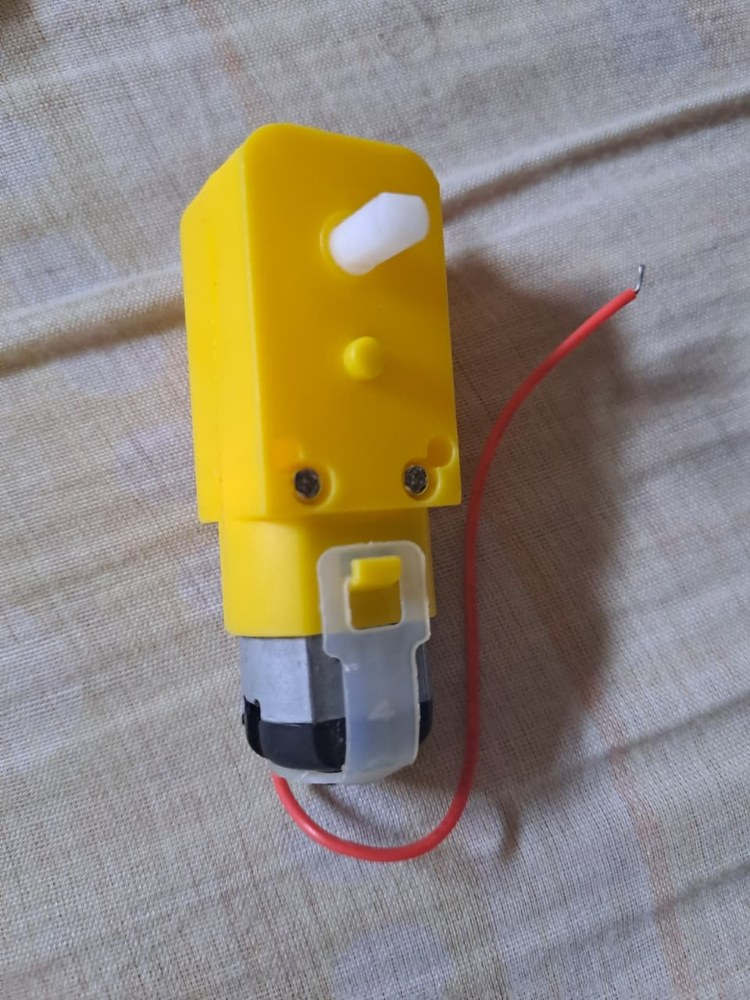
\includegraphics[height=5.2cm]{photos/moteur_tt.jpg}
  \caption{Moteur à réducteur (identique pour les deux côtés)}
\end{subfigure}\hspace{1cm}
\begin{subfigure}[b]{0.3\linewidth}\centering
  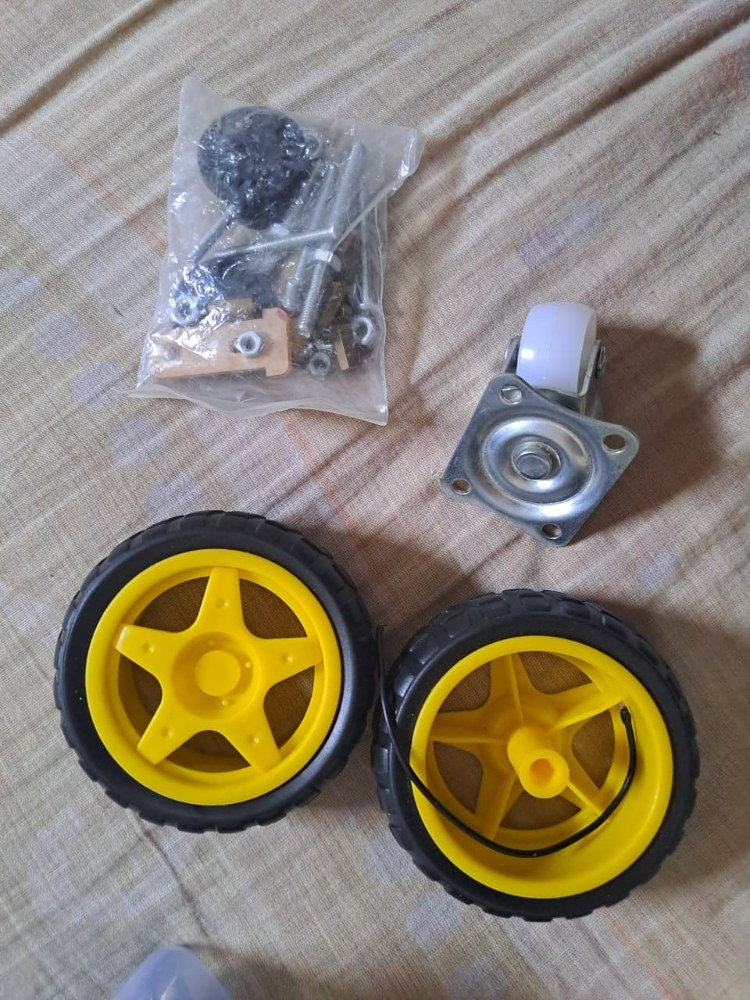
\includegraphics[height=5.2cm]{photos/roues.jpg}
  \caption{Roues, roue folle et visserie}
\end{subfigure}
\caption{Les deux moteurs à courant continu et les éléments de roulement}
\label{fig:moteurs}
\end{figure}

% ------------------------------------------------------------------------------------------------
\section{Capteurs infrarouges}

Deux capteurs infrarouges à réflexion, orientés vers le sol, permettent de suivre la piste (figure~\ref{fig:ir}).
Chaque module comporte une LED émettrice infrarouge, une photodiode réceptrice, un comparateur LM393 et un
potentiomètre de réglage du seuil. Le sol clair réfléchit le rayonnement infrarouge, alors que le ruban noir
l'absorbe : la sortie numérique OUT change donc d'état lorsque le capteur passe au-dessus du ruban. Le
potentiomètre permet d'ajuster le seuil à la hauteur du capteur et à l'éclairage.

\begin{figure}[H]
\centering
\begin{subfigure}[b]{0.3\linewidth}\centering
  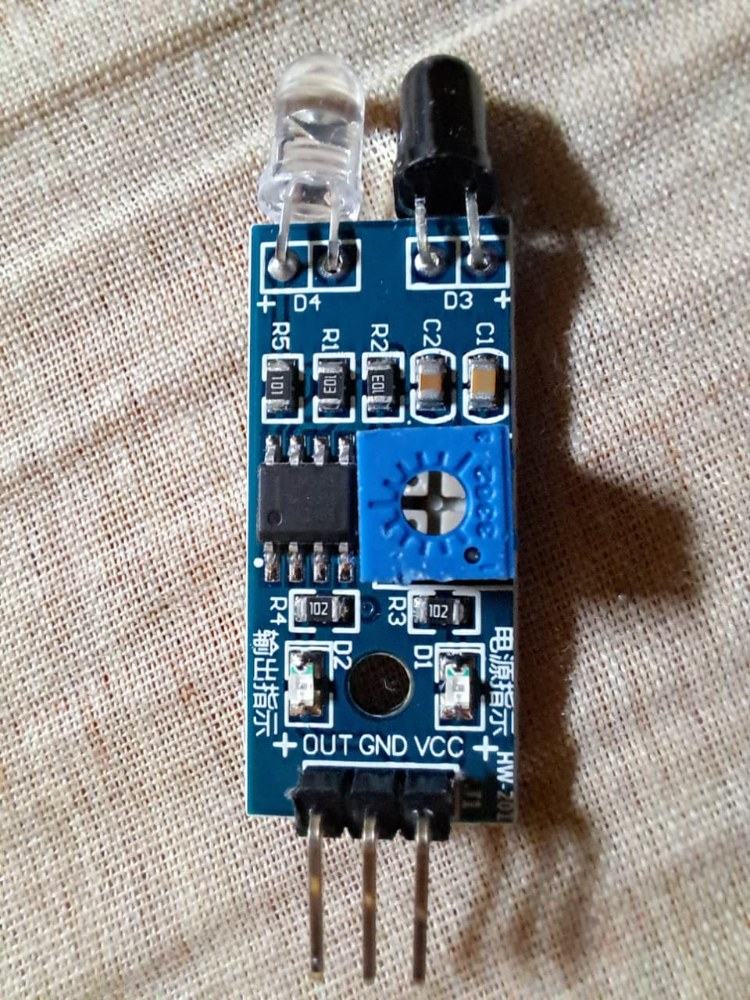
\includegraphics[height=5.6cm]{photos/ir_face.jpg}
  \caption{Face avant : LED IR, photodiode, potentiomètre, broches OUT / GND / VCC}
\end{subfigure}\hspace{1cm}
\begin{subfigure}[b]{0.3\linewidth}\centering
  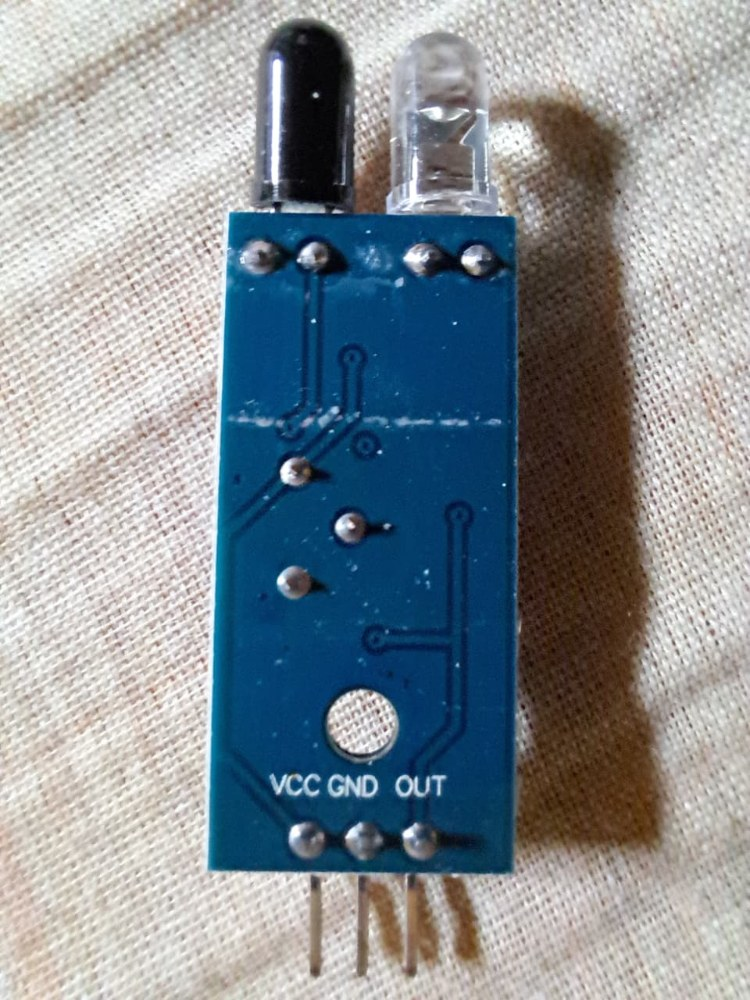
\includegraphics[height=5.6cm]{photos/ir_dos.jpg}
  \caption{Face arrière}
\end{subfigure}
\caption{Capteurs infrarouges gauche et droit (deux modules identiques)}
\label{fig:ir}
\end{figure}

Les deux capteurs sont placés de part et d'autre du ruban. Tant que tous deux voient le sol clair, la voiture
avance tout droit ; lorsque l'un d'eux détecte le ruban, la ligne s'est décalée de ce côté et la voiture tourne
dans cette direction (tableau~\ref{tab:suivi}).

\begin{table}[H]
\centering\small
\caption{Logique de suivi de ligne à deux capteurs}
\label{tab:suivi}
\begin{tabular}{ccl}
\toprule
\textbf{IR gauche} & \textbf{IR droit} & \textbf{Action} \\
\midrule
sol clair & sol clair & Avancer tout droit \\
ruban noir & sol clair & Tourner à gauche \\
sol clair & ruban noir & Tourner à droite \\
ruban noir & ruban noir & S'arrêter (croisement ou fin de piste) \\
\bottomrule
\end{tabular}
\end{table}

% ------------------------------------------------------------------------------------------------
\section{Capteur ultrasonique HC-SR04}

Le HC-SR04 mesure la distance à l'obstacle situé devant la voiture par temps de vol d'une onde ultrasonore
(figure~\ref{fig:hcsr04})~\cite{hcsr04}. Une impulsion d'au moins 10 µs sur la broche \textbf{Trig} déclenche
l'émission d'une salve de huit impulsions à 40 kHz ; la broche \textbf{Echo} passe alors à l'état haut pendant
une durée $t$ égale au temps d'aller-retour de l'onde. La distance s'en déduit par :
\begin{equation}
  d = \frac{v_{son}\, t}{2} \approx \frac{343~\text{m/s} \times t}{2}
  \quad\Longleftrightarrow\quad d~[\text{cm}] \approx \frac{t~[\text{µs}]}{58}
\end{equation}
Le capteur mesure de 2 cm à 4 m environ, avec un cône de détection d'une quinzaine de degrés. Il est alimenté en
5 V et ses quatre broches sont : \textbf{VCC}, \textbf{Trig}, \textbf{Echo} et \textbf{GND}.

\begin{figure}[H]
\centering
\begin{tikzpicture}
  \node[anchor=south west,inner sep=0] (img) at (0,0) {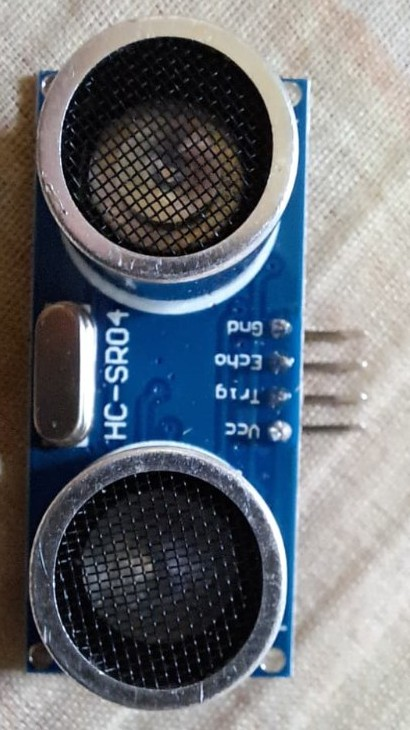
\includegraphics[width=3.9cm]{photos/hcsr04_crop.jpg}};
  \begin{scope}[x={(img.south east)},y={(img.north west)}]
    \draw[annot] (0.878,0.544) -- (1.25,0.70) node[lab,right] {\textbf{GND} — masse};
    \draw[annot] (0.878,0.501) -- (1.25,0.59) node[lab,right] {\textbf{Echo} $\rightarrow$ D13 (durée de l'écho)};
    \draw[annot] (0.878,0.459) -- (1.25,0.48) node[lab,right] {\textbf{Trig} $\leftarrow$ D12 (impulsion de 10 µs)};
    \draw[annot] (0.878,0.416) -- (1.25,0.37) node[lab,right] {\textbf{VCC} — alimentation 5 V};
    \draw[annot] (0.40,0.80) -- (-0.15,0.80) node[lab,left] {Transducteur ultrasonore\\(40 kHz)};
    \draw[annot] (0.38,0.22) -- (-0.15,0.22) node[lab,left] {Transducteur ultrasonore\\(40 kHz)};
    \draw[annot] (0.16,0.49) -- (-0.15,0.51) node[lab,left] {Oscillateur à quartz};
  \end{scope}
\end{tikzpicture}
\caption{Capteur ultrasonique HC-SR04 et ses quatre broches}
\label{fig:hcsr04}
\end{figure}

% ------------------------------------------------------------------------------------------------
\section{ESP32-CAM}

L'ESP32-CAM (modèle AI-Thinker) est un module très compact qui associe un microcontrôleur ESP32 à double cœur
(240 MHz) doté du Wi-Fi et du Bluetooth, 4 Mo de mémoire PSRAM, un connecteur de caméra, un lecteur de carte
microSD et une LED de flash~\cite{esp32cam}. Le module de notre prototype porte un capteur OV3660 ; il ne
possède pas de port USB et se programme à travers sa carte support \textbf{ESP32-CAM-MB}, qui lui fournit une
interface USB-série (CH340), des boutons de démarrage et de réinitialisation, et l'alimentation 5 V
(figure~\ref{fig:esp32cam}).

\begin{figure}[H]
\centering
\begin{subfigure}[b]{0.31\linewidth}\centering
  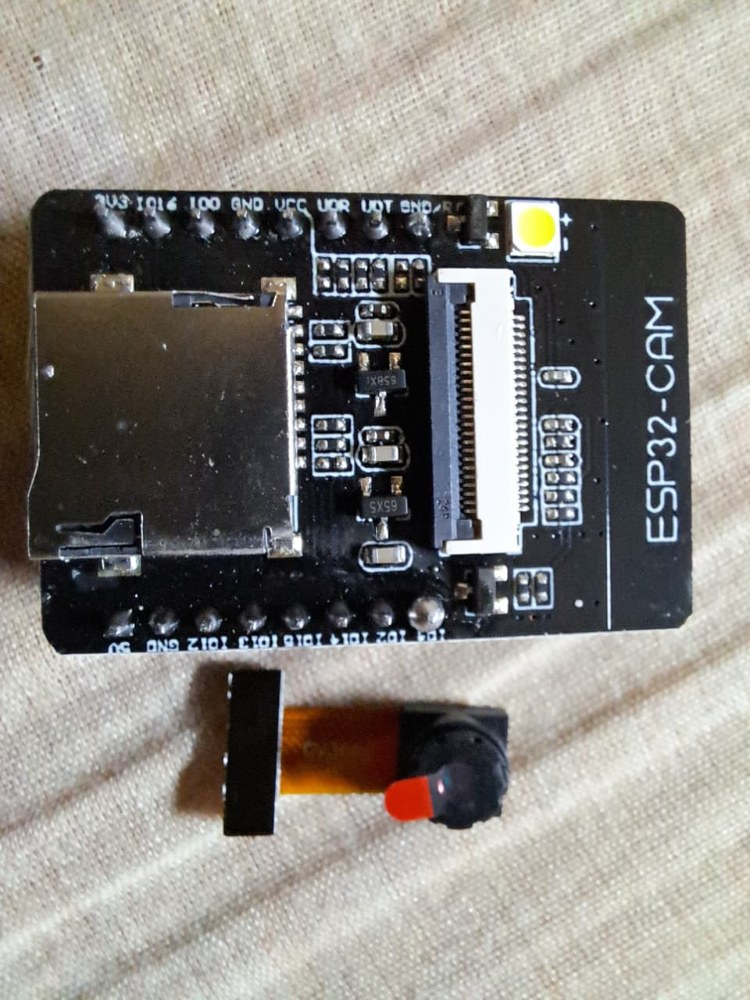
\includegraphics[height=5.4cm]{photos/esp32cam.jpg}
  \caption{Module ESP32-CAM et sa caméra}
\end{subfigure}\hfill
\begin{subfigure}[b]{0.31\linewidth}\centering
  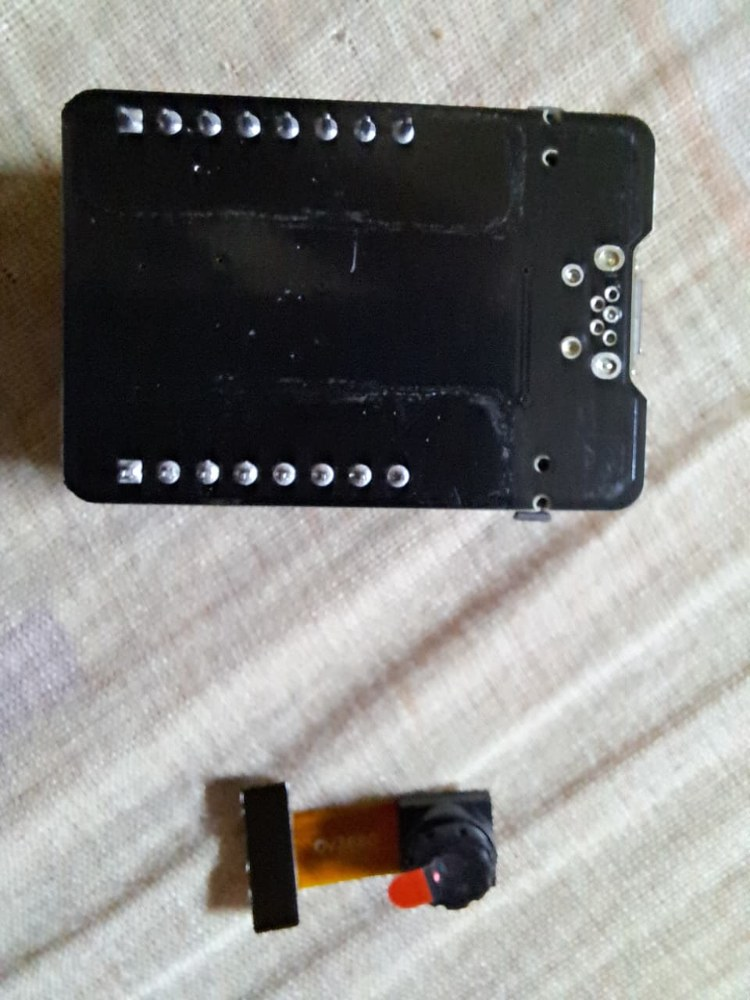
\includegraphics[height=5.4cm]{photos/esp32cam_mb.jpg}
  \caption{Carte support ESP32-CAM-MB}
\end{subfigure}\hfill
\begin{subfigure}[b]{0.31\linewidth}\centering
  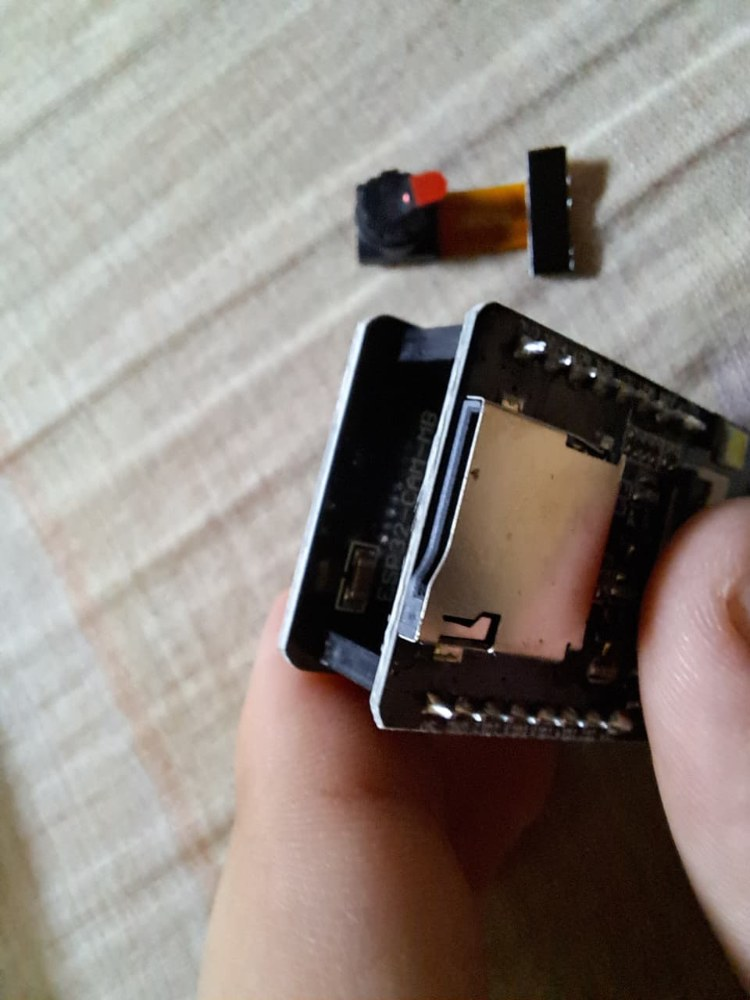
\includegraphics[height=5.4cm]{photos/esp32cam_assemblage.jpg}
  \caption{Assemblage des deux cartes}
\end{subfigure}
\caption{Module ESP32-CAM et son support ESP32-CAM-MB}
\label{fig:esp32cam}
\end{figure}

La caméra exécute le programme d'exemple \textit{CameraWebServer} d'Espressif. Celui-ci se connecte au réseau Wi-Fi
local et expose deux services HTTP : un flux vidéo MJPEG sur le port 81 (\texttt{/stream}) et une interface de
réglage sur le port 80 (\texttt{/status}, \texttt{/control}) pour la résolution, la qualité JPEG, le flash, le
retournement ou le miroir de l'image. Nous utilisons la résolution VGA (640\,$\times$\,480).

Deux particularités du montage ont eu des conséquences sur le logiciel :
\begin{itemize}
  \item \textbf{L'adresse IP est attribuée dynamiquement} par le point d'accès. Le serveur retrouve donc la caméra
        automatiquement (dernière adresse connue, puis balayage du sous-réseau), comme décrit au chapitre~4.
  \item \textbf{La caméra est montée sur la tranche}, à l'avant droit de la voiture : l'image arrive tournée de
        90°. Le capteur ne sait que retourner ou inverser l'image ; la rotation est donc réalisée par le serveur
        avant l'affichage et la détection.
\end{itemize}

% ------------------------------------------------------------------------------------------------
\section{Système d'alimentation}

L'alimentation du prototype est volontairement simple et repose sur deux sources séparées, sans circuit de
régulation supplémentaire (figure~\ref{fig:alimentation}) :
\begin{itemize}
  \item \textbf{quatre piles alcalines AA} de 1,5 V (Duracell), soit environ 6 V, reliées à l'entrée VS du L298N à
        travers un interrupteur marche/arrêt : elles alimentent uniquement les moteurs ;
  \item \textbf{une batterie externe USB 5 V}, qui alimente la caméra ESP32-CAM par sa carte MB ainsi que
        l'électronique de commande. Le rail logique 5 V et la masse sont communs à l'Arduino, au L298N, au HC-SR04
        et aux deux capteurs infrarouges.
\end{itemize}

\begin{figure}[H]
\centering
\begin{subfigure}[b]{0.3\linewidth}\centering
  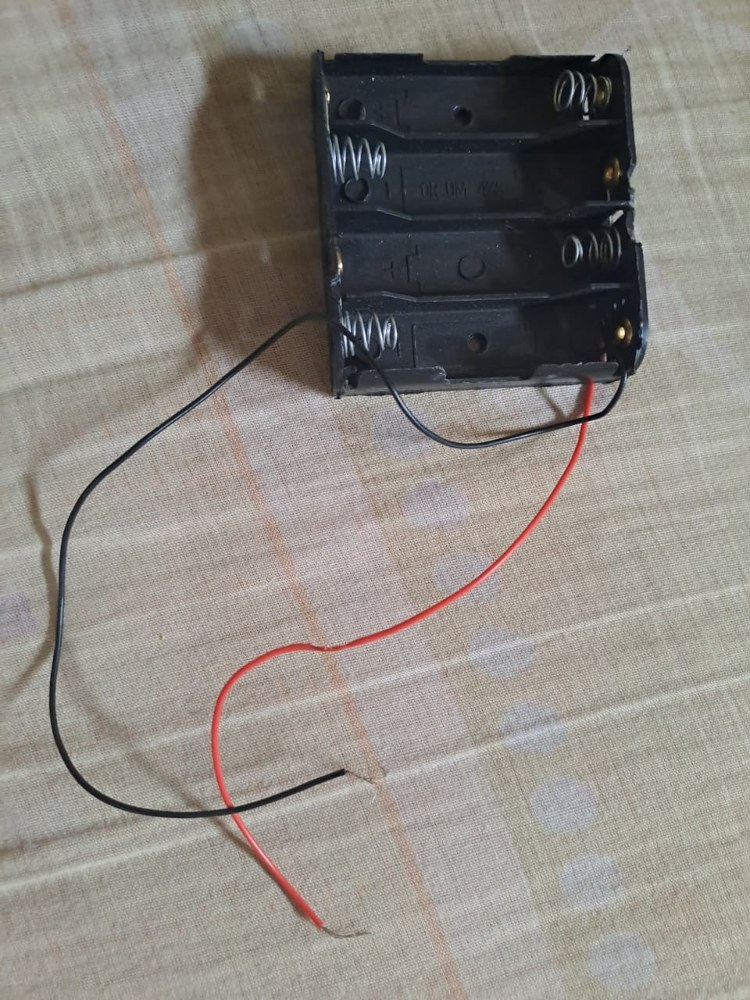
\includegraphics[height=4.6cm]{photos/piles_aa.jpg}
  \caption{Support de 4 piles AA}
\end{subfigure}\hspace{0.8cm}
\begin{subfigure}[b]{0.3\linewidth}\centering
  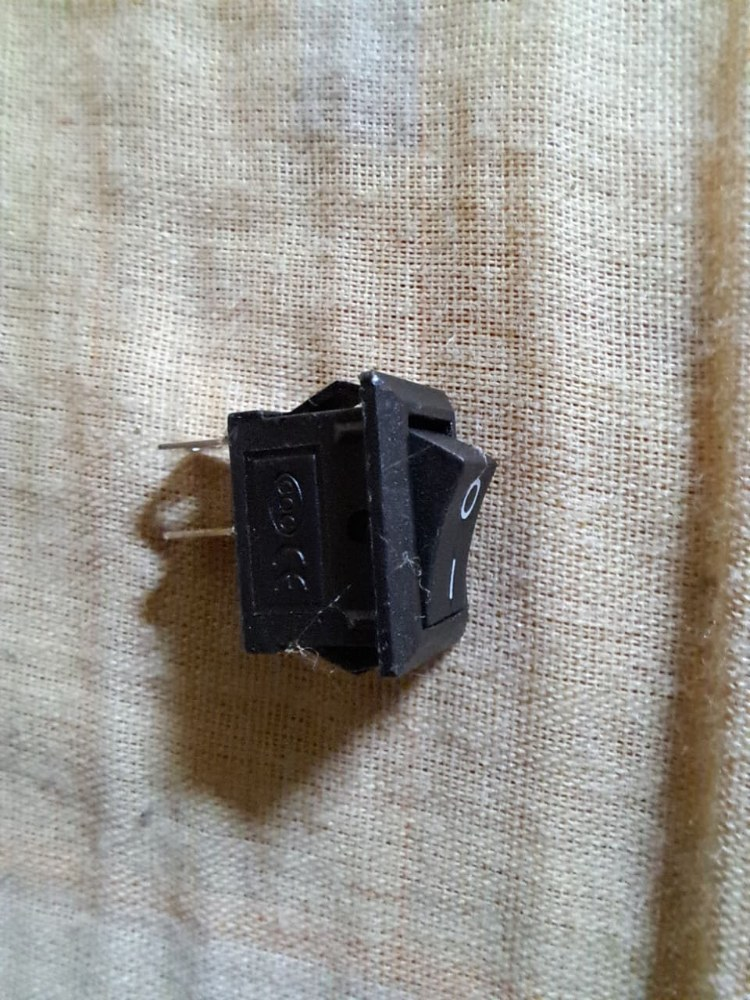
\includegraphics[height=4.6cm]{photos/interrupteur.jpg}
  \caption{Interrupteur marche / arrêt}
\end{subfigure}
\caption{Éléments du circuit d'alimentation des moteurs}
\label{fig:alimentation}
\end{figure}

Cette séparation est volontaire. Au démarrage et lors des changements de sens, les moteurs appellent des pointes
de courant qui font chuter la tension ; partagée avec la caméra, cette chute provoquerait des redémarrages de
l'ESP32 (\textit{brownout}), particulièrement sensible pendant les émissions Wi-Fi. Le tableau~\ref{tab:conso}
donne des ordres de grandeur des consommations.

\begin{table}[H]
\centering\small
\caption{Ordres de grandeur des consommations (valeurs typiques des fiches techniques)}
\label{tab:conso}
\begin{tabular}{lll}
\toprule
\textbf{Élément} & \textbf{Source} & \textbf{Consommation typique} \\
\midrule
2 moteurs TT & piles AA (via L298N) & 2 $\times$ 100 à 250 mA en roulage, davantage au démarrage \\
Arduino UNO & batterie USB & $\approx$ 50 mA \\
HC-SR04 & rail 5 V (Arduino) & $\approx$ 15 mA \\
2 capteurs IR & rail 5 V (Arduino) & 2 $\times$ $\approx$ 20 mA \\
ESP32-CAM (diffusion Wi-Fi) & batterie USB & $\approx$ 200 à 300 mA, plus avec le flash \\
\bottomrule
\end{tabular}
\end{table}

Cette solution a l'avantage de la simplicité : les piles se remplacent facilement et la batterie externe se
recharge par USB. Compte tenu de la chute de tension du L298N, une batterie lithium de 7,4 V permettrait
toutefois aux moteurs de recevoir une tension plus proche de leur valeur nominale et à la voiture d'aller plus
vite.

% ------------------------------------------------------------------------------------------------
\section{Schéma de câblage}

Le schéma de câblage complet est donné par la figure~\ref{fig:montage}, et le tableau~\ref{tab:liaisons} en
reprend les liaisons.

\begin{figure}[H]
\centering
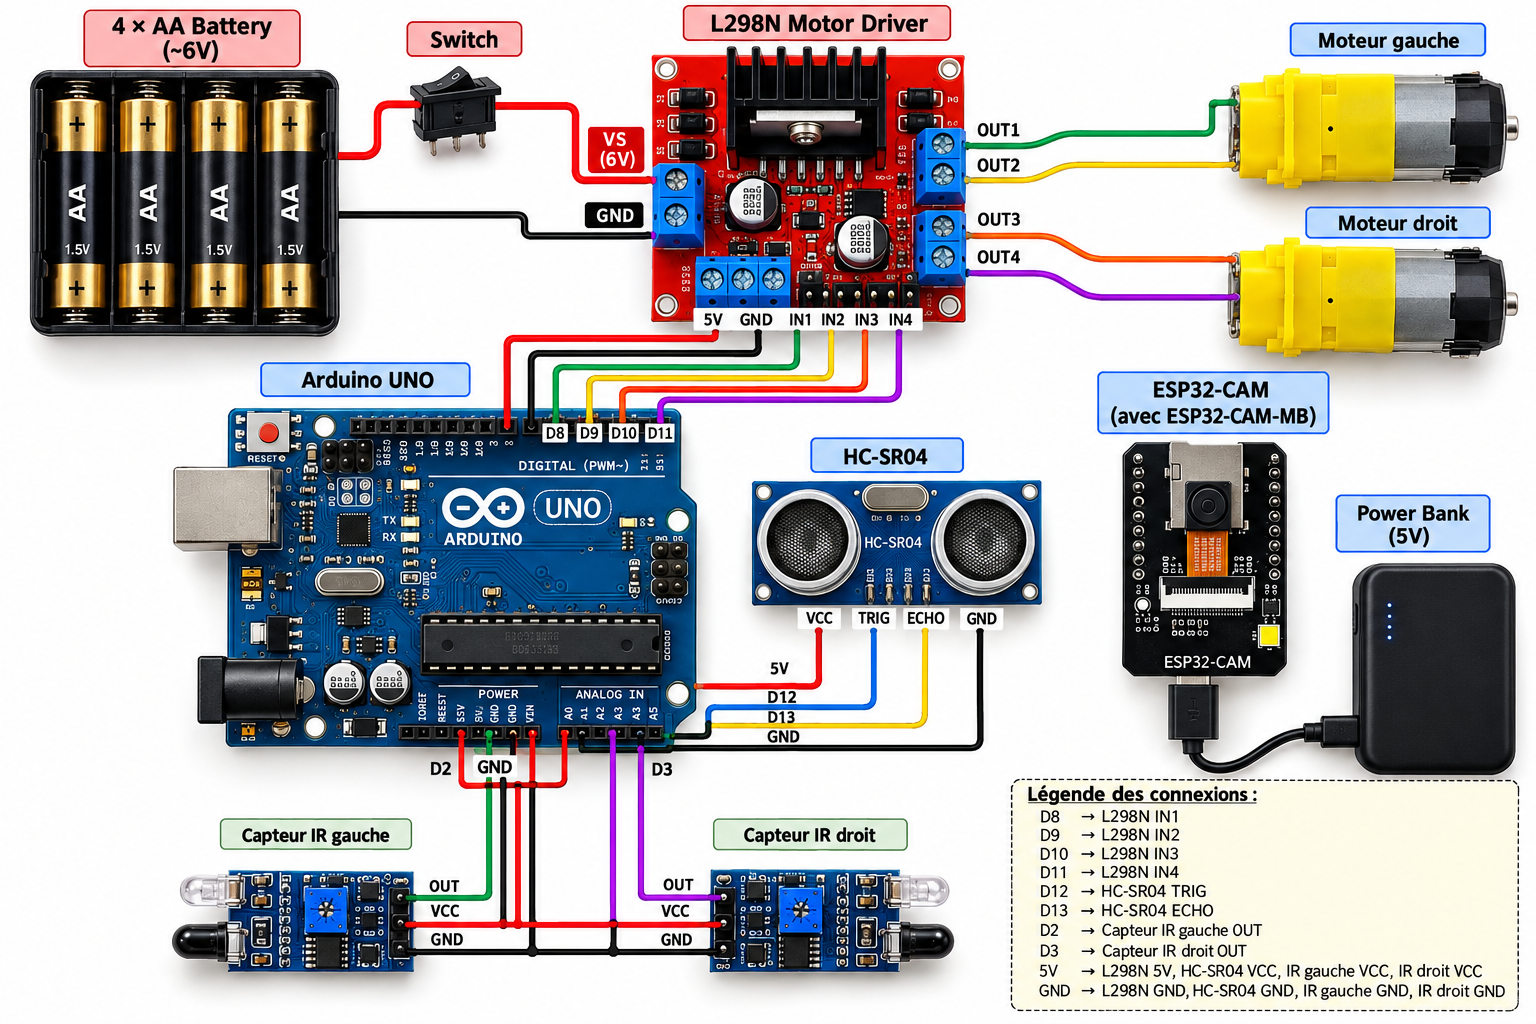
\includegraphics[width=\linewidth]{montage.png}
\caption{Schéma de câblage du prototype}
\label{fig:montage}
\end{figure}

\begin{table}[H]
\centering\small
\caption{Liaisons du schéma de câblage}
\label{tab:liaisons}
\begin{tabular}{ll}
\toprule
\textbf{De} & \textbf{Vers} \\
\midrule
Piles AA (+) $\rightarrow$ interrupteur & L298N VS (6 V) \\
Piles AA ($-$) & L298N GND \\
L298N OUT1, OUT2 / OUT3, OUT4 & Moteur gauche / moteur droit \\
Arduino D8, D9, D10, D11 & L298N IN1, IN2, IN3, IN4 \\
Arduino D12 / D13 & HC-SR04 Trig / Echo \\
Arduino D2 / D3 & Sortie OUT du capteur IR gauche / droit \\
Arduino 5 V & L298N 5 V, HC-SR04 VCC, VCC des capteurs IR \\
Arduino GND & L298N GND, HC-SR04 GND, GND des capteurs IR \\
Batterie externe (USB 5 V) & ESP32-CAM-MB $\rightarrow$ ESP32-CAM ; Arduino UNO (USB) \\
\bottomrule
\end{tabular}
\end{table}

% ------------------------------------------------------------------------------------------------
\section{Réalisation physique du prototype}

Le prototype est monté sur un châssis en acrylique à deux roues motrices et une roue folle
(figure~\ref{fig:chassis}). Les composants sont disposés pour garder un centre de gravité bas et laisser à la
caméra un champ de vision dégagé (figure~\ref{fig:prototype}) :
\begin{itemize}
  \item à l'avant, le HC-SR04 est fixé au centre du pare-chocs, encadré par les deux capteurs infrarouges orientés
        vers le sol, à quelques millimètres de la piste ;
  \item l'ESP32-CAM, montée sur la tranche avec sa carte MB, occupe l'angle avant ; sa caméra regarde vers
        l'avant, à hauteur de la piste, ce qui donne le point de vue d'un conducteur ;
  \item l'Arduino UNO est placé au centre du châssis, l'interrupteur juste derrière ;
  \item à l'arrière, la batterie externe porte le module L298N, au plus près des moteurs.
\end{itemize}

\begin{figure}[H]
\centering
\begin{subfigure}[b]{0.38\linewidth}\centering
  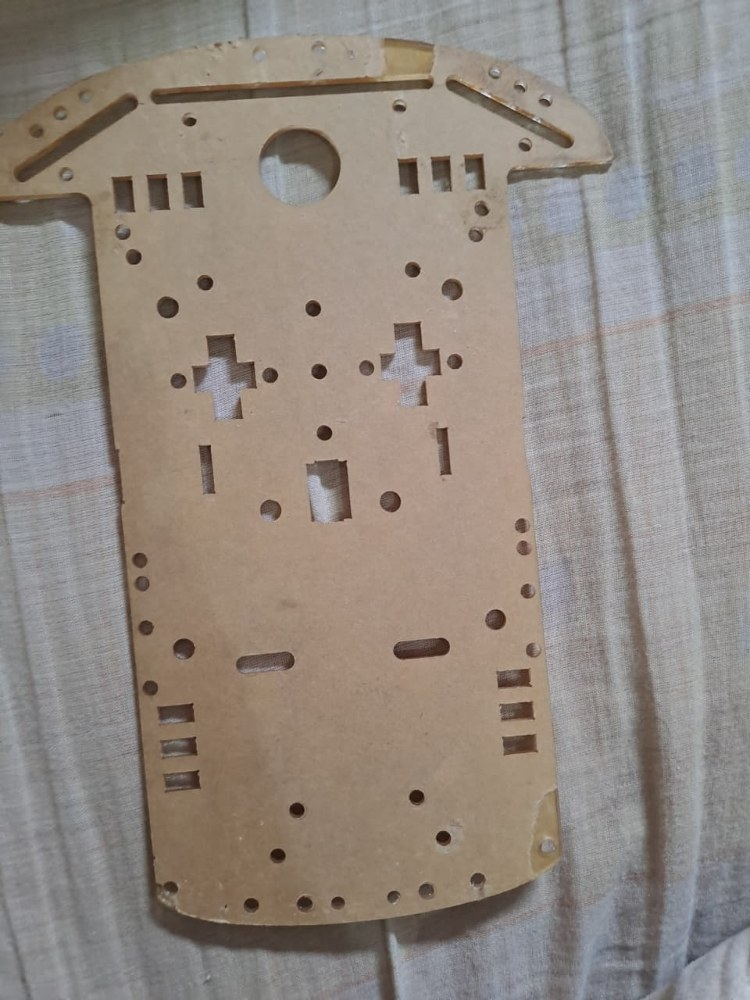
\includegraphics[height=5cm]{photos/chassis.jpg}
  \caption{Châssis en acrylique}
\end{subfigure}\hspace{0.8cm}
\begin{subfigure}[b]{0.38\linewidth}\centering
  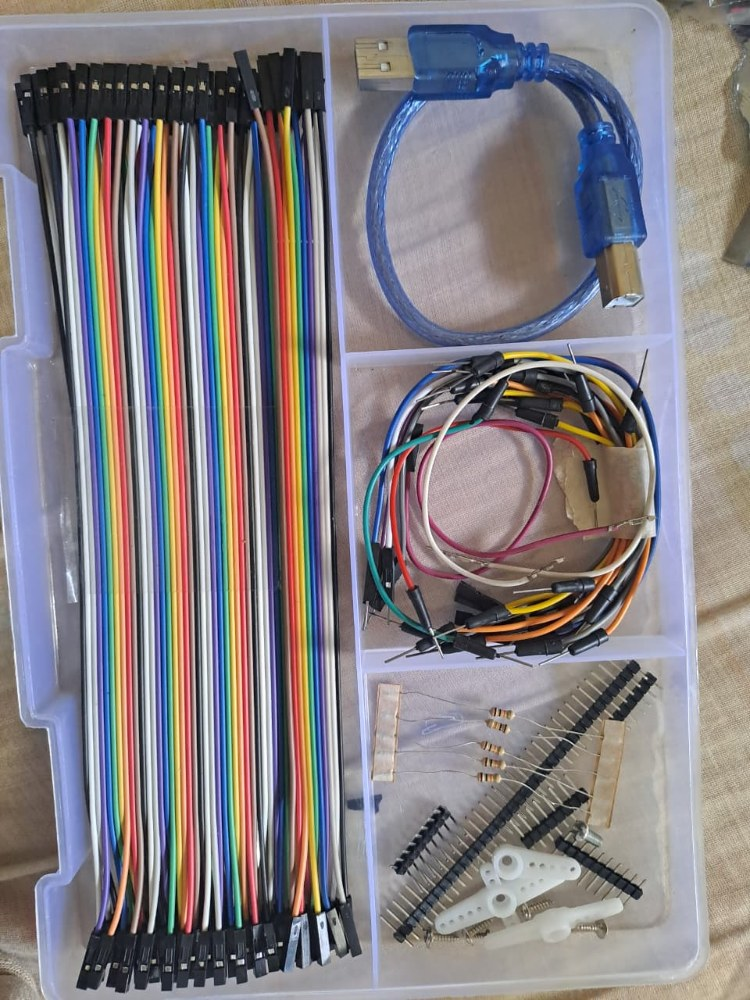
\includegraphics[height=5cm]{photos/fils_dupont.jpg}
  \caption{Fils de liaison Dupont}
\end{subfigure}
\caption{Éléments mécaniques et de liaison}
\label{fig:chassis}
\end{figure}

\begin{figure}[H]
\centering
\begin{subfigure}[b]{0.49\linewidth}\centering
  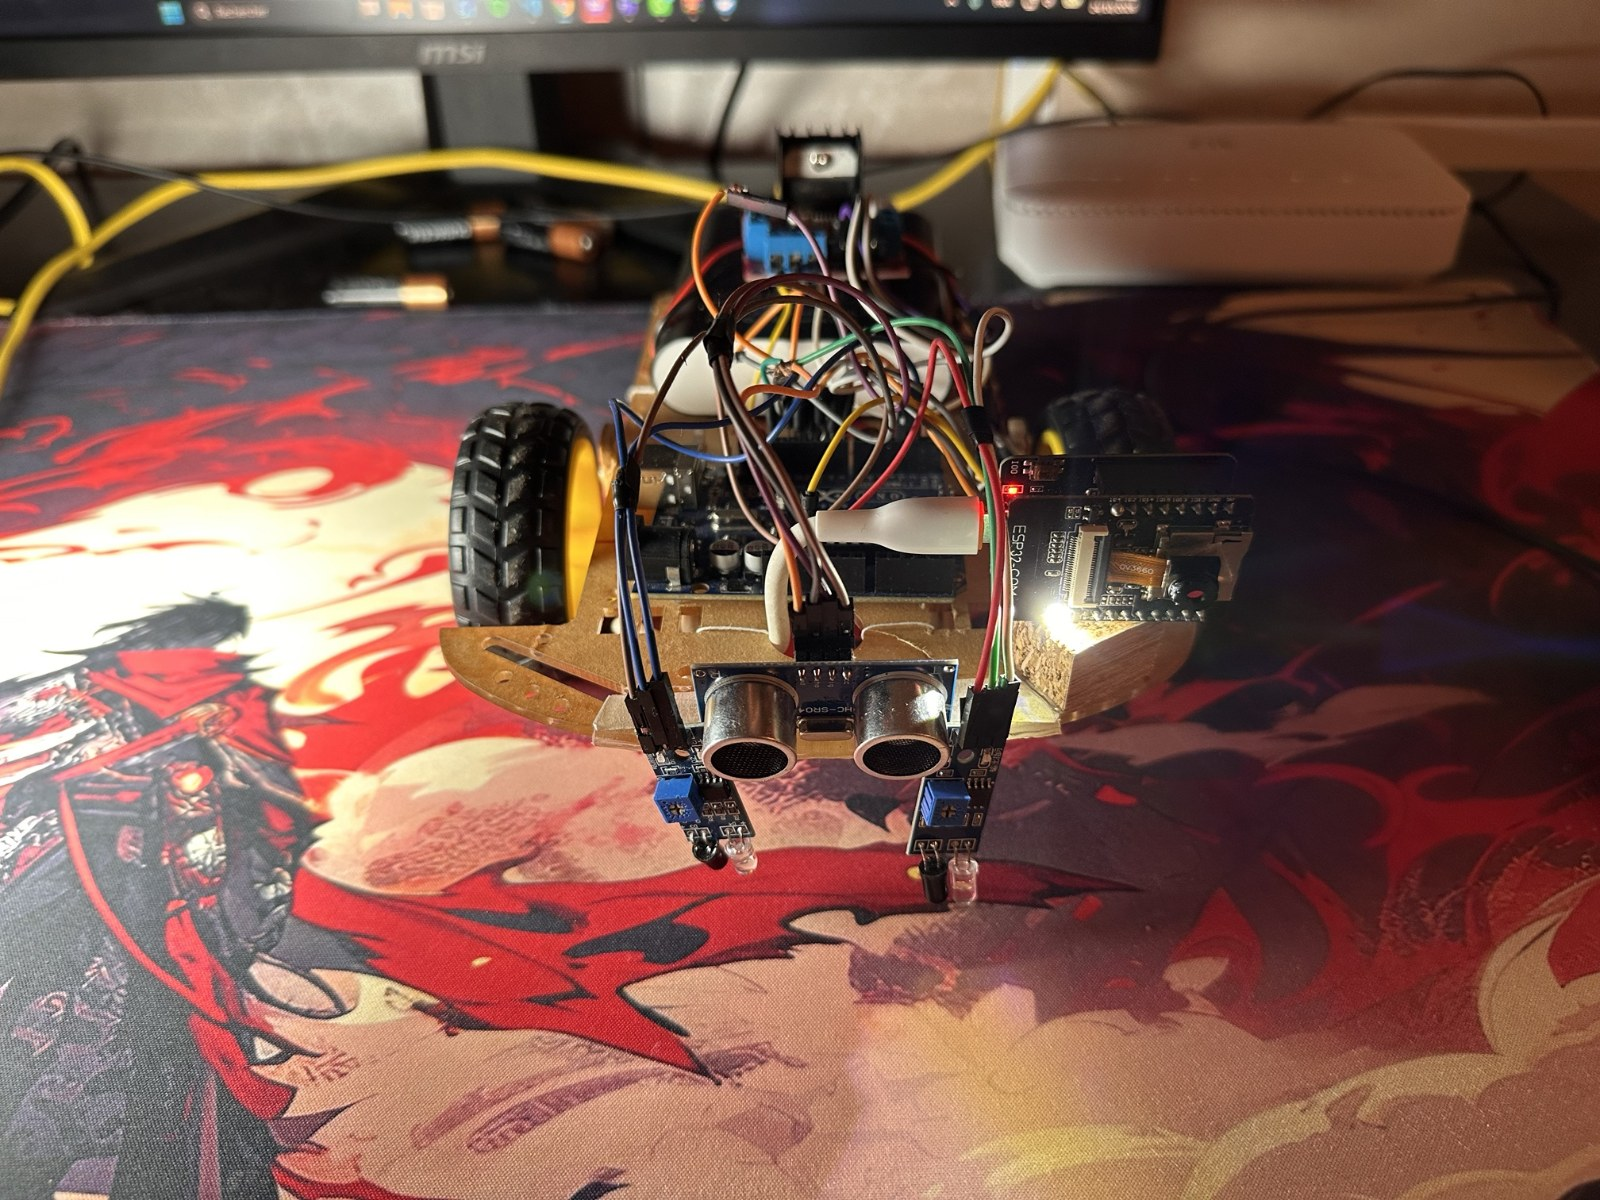
\includegraphics[width=\linewidth]{photos/prototype_avant.jpg}
  \caption{Vue avant : HC-SR04, capteurs IR et ESP32-CAM}
\end{subfigure}\hfill
\begin{subfigure}[b]{0.49\linewidth}\centering
  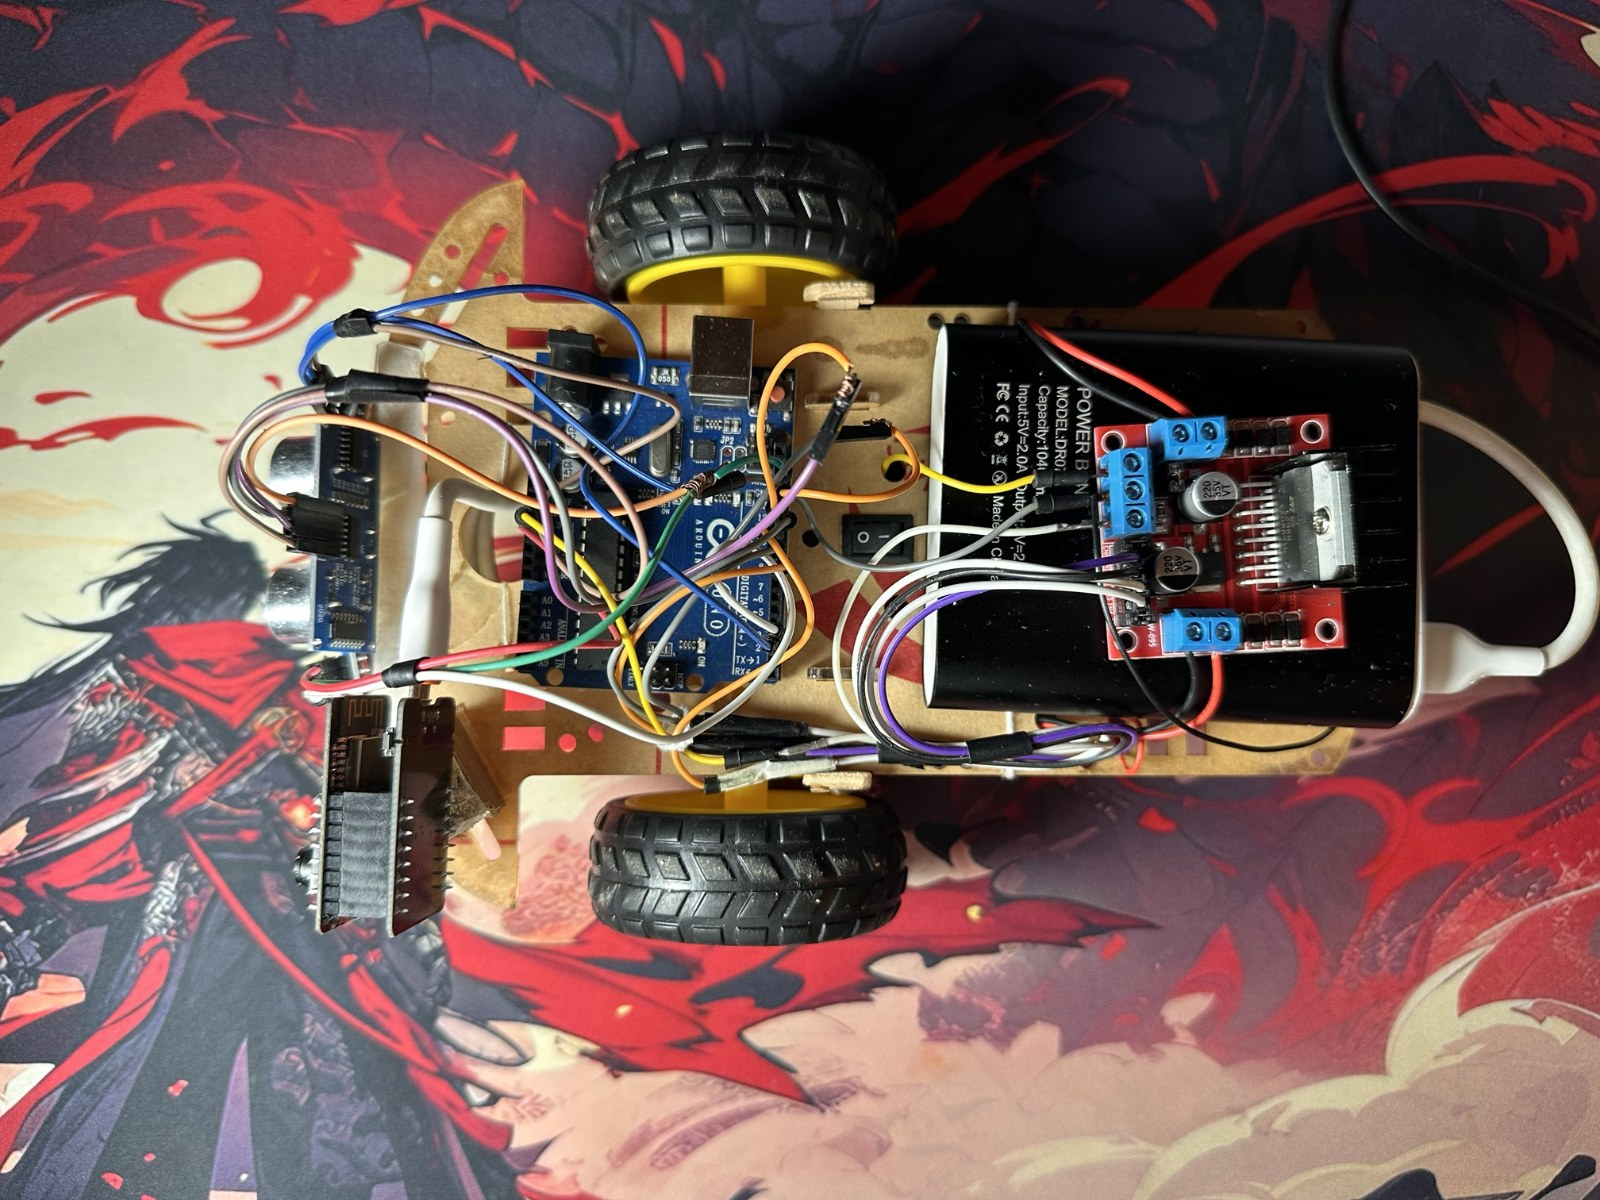
\includegraphics[width=\linewidth]{photos/prototype_dessus.jpg}
  \caption{Vue de dessus : Arduino, L298N et batterie externe}
\end{subfigure}
\caption{Prototype assemblé}
\label{fig:prototype}
\end{figure}

\subsection*{Logique de commande embarquée}
Le programme de l'Arduino combine le suivi de ligne et la sécurité frontale. À chaque itération, il mesure la
distance frontale ; si un obstacle est trop proche, il arrête les moteurs, sinon il applique la logique de suivi
de ligne du tableau~\ref{tab:suivi}. L'algorithme~\ref{alg:commande} en résume le principe.

\begin{algorithm}[H]
\caption{Principe de la boucle de commande de l'Arduino}
\label{alg:commande}
\begin{algorithmic}[1]
\Loop
  \State $d \gets$ distance mesurée par le HC-SR04
  \If{$d < d_{\text{sécurité}}$} \State arrêter les deux moteurs \Comment{obstacle devant la voiture}
  \Else
    \State $g \gets$ état du capteur IR gauche, \ $r \gets$ état du capteur IR droit
    \If{$g = $ sol clair \textbf{et} $r = $ sol clair} \State avancer
    \ElsIf{$g = $ ruban} \State tourner à gauche \Comment{moteur gauche ralenti}
    \ElsIf{$r = $ ruban} \State tourner à droite \Comment{moteur droit ralenti}
    \Else \State s'arrêter
    \EndIf
  \EndIf
\EndLoop
\end{algorithmic}
\end{algorithm}

\subsection*{Piste d'essai}
La piste est une boucle fermée tracée au ruban adhésif noir sur un carrelage clair, aux angles arrondis
(figure~\ref{fig:piste}). Ses dimensions ne sont pas figées : la piste est retracée à chaque séance d'essai selon
l'espace disponible, et sa géométrie peut être redéfinie dans l'éditeur de piste de l'application. Deux obstacles
y sont placés : une \textbf{colonne} rayée à sommet noir
et une \textbf{boîte} de couleur crème. Ce sont les deux classes que le modèle du prototype doit reconnaître
(chapitre~3). Les six points de passage A à F de la piste, définis dans l'application, peuvent recevoir des
marqueurs ArUco imprimés que la caméra lit pour localiser la voiture.

\begin{figure}[H]
\centering
\begin{subfigure}[b]{0.52\linewidth}\centering
  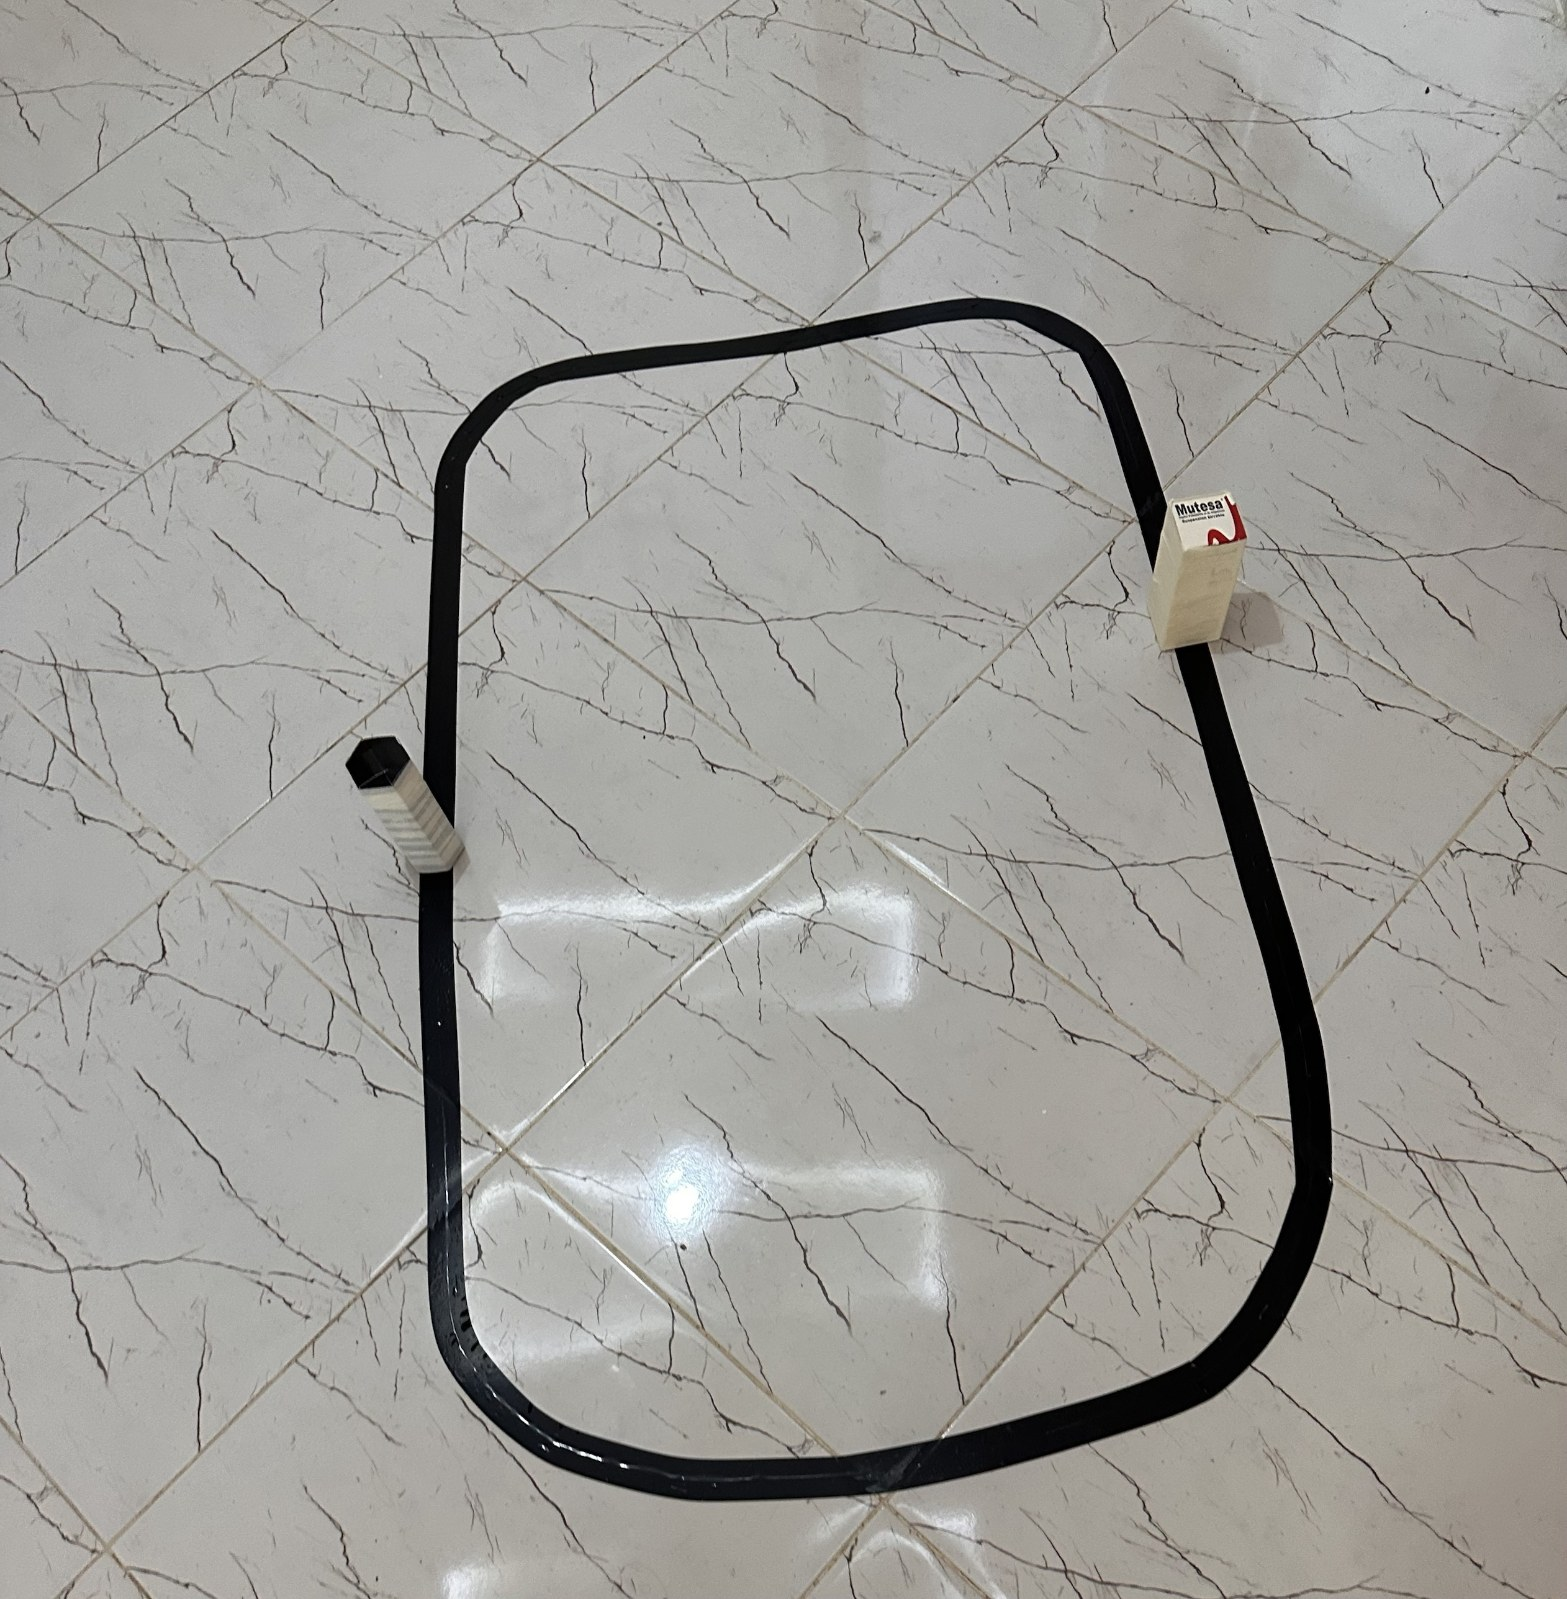
\includegraphics[height=7.2cm]{photos/piste.jpg}
  \caption{Vue de dessus de la piste et des deux obstacles}
\end{subfigure}\hfill
\begin{subfigure}[b]{0.42\linewidth}\centering
  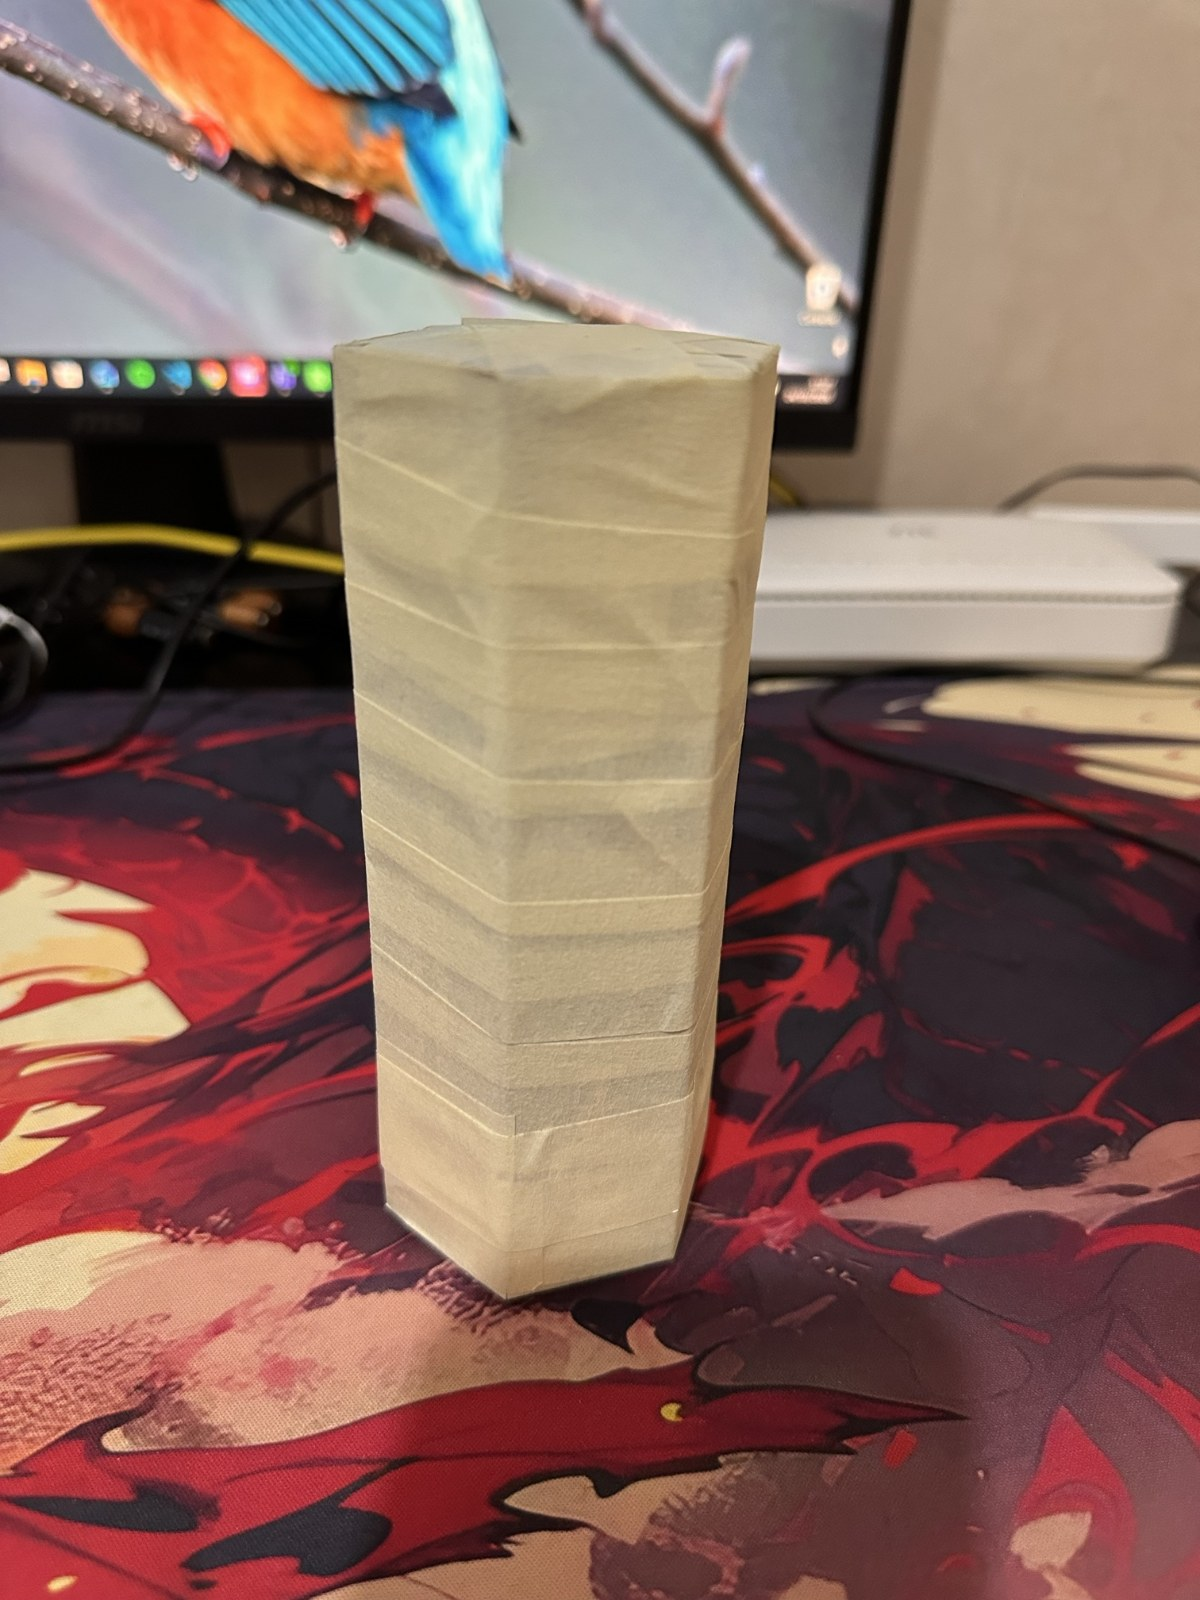
\includegraphics[height=7.2cm]{photos/obstacle_colonne.jpg}
  \caption{Obstacle « colonne »}
\end{subfigure}
\caption{Piste d'essai et obstacles du prototype}
\label{fig:piste}
\end{figure}

\chapconclusion
Ce chapitre a présenté la réalisation matérielle du prototype : une architecture en deux sous-systèmes
indépendants, l'un pour la commande (Arduino, L298N, moteurs, capteurs infrarouges et ultrasonique), l'autre pour la
vision (ESP32-CAM). Le prototype suit sa piste de façon autonome et fournit, par sa caméra, les images que les
modèles d'intelligence artificielle du chapitre suivant vont analyser.

\chapter{Conception et développement du modèle d'intelligence artificielle}

\chapintro
Ce chapitre présente la partie « intelligence » du système : les modèles de vision par ordinateur qui détectent les
obstacles dans les images. Après un rappel des principes de la vision par ordinateur et de la détection d'objets,
nous présentons la famille de modèles YOLO26 et l'environnement Ultralytics. Nous décrivons ensuite la
préparation des deux jeux de données (routes réelles et piste du prototype), le développement et l'entraînement
des modèles, l'exploitation de leurs prédictions (localisation, distance, gravité, priorité) et enfin
l'évaluation de leurs performances.

% =================================================================================================
\section{Introduction à la vision par ordinateur}

\subsection{Principes de la vision par ordinateur}
La vision par ordinateur vise à extraire automatiquement de l'information d'images ou de vidéos. Pour une machine,
une image couleur est un tableau de nombres de taille $H \times W \times 3$ (hauteur, largeur, trois canaux rouge,
vert et bleu). Les méthodes classiques reposaient sur des descripteurs conçus à la main (contours, histogrammes de
gradients, couleurs). Depuis 2012, les \textbf{réseaux de neurones convolutifs} (CNN) apprennent eux-mêmes ces
descripteurs à partir d'exemples annotés : les premières couches détectent des motifs simples (bords, textures), les
couches profondes des structures de plus en plus abstraites (roues, visages, objets entiers).

Une chaîne de vision comporte généralement les étapes de la figure~\ref{fig:chaine-vision} : acquisition de
l'image, prétraitement (redimensionnement, normalisation), inférence du modèle, post-traitement des prédictions et
exploitation du résultat par l'application.

\begin{figure}[H]
\centering
\resizebox{\linewidth}{!}{%
\begin{tikzpicture}[node distance=0.55cm]
  \node[bloco,minimum width=2.4cm] (a) {Acquisition\\\scriptsize caméra, vidéo};
  \node[bloc,minimum width=2.6cm,right=of a] (b) {Prétraitement\\\scriptsize rotation, \textit{letterbox}};
  \node[blocg,minimum width=2.6cm,right=of b] (c) {Inférence\\\scriptsize réseau YOLO26};
  \node[bloc,minimum width=2.8cm,right=of c] (d) {Post-traitement\\\scriptsize seuil, coordonnées};
  \node[blocv,minimum width=2.8cm,right=of d] (e) {Exploitation\\\scriptsize distance, gravité, carte};
  \foreach \x/\y in {a/b,b/c,c/d,d/e} \draw[fleche] (\x) -- (\y);
\end{tikzpicture}}
\caption{Chaîne de traitement d'un système de vision par ordinateur}
\label{fig:chaine-vision}
\end{figure}

\subsection{Détection d'objets et segmentation d'images}
On distingue plusieurs tâches de complexité croissante :
\begin{itemize}
  \item la \textbf{classification}, qui attribue une étiquette à l'image entière (« il y a un cône ») ;
  \item la \textbf{détection d'objets}, qui localise chaque objet par une \emph{boîte englobante}
        $(x_1, y_1, x_2, y_2)$ et lui associe une classe et un score de confiance ;
  \item la \textbf{segmentation}, qui attribue une classe à chaque pixel. La segmentation d'instances distingue en
        plus les objets individuels et fournit leur contour exact (\emph{masque}).
\end{itemize}
La détection d'objets est la tâche adaptée à notre besoin : elle indique quels obstacles sont présents, où ils se
trouvent dans l'image et avec quelle confiance, tout en restant assez rapide pour le temps réel. Nous avons
cependant utilisé la segmentation à une autre étape : pour \emph{annoter} automatiquement les images de notre piste,
le modèle de segmentation SAM~2~\cite{ravi2024sam2} a produit le masque de chaque obstacle, dont la boîte englobante
se déduit directement (figure~\ref{fig:det-seg}).

\begin{figure}[H]
\centering
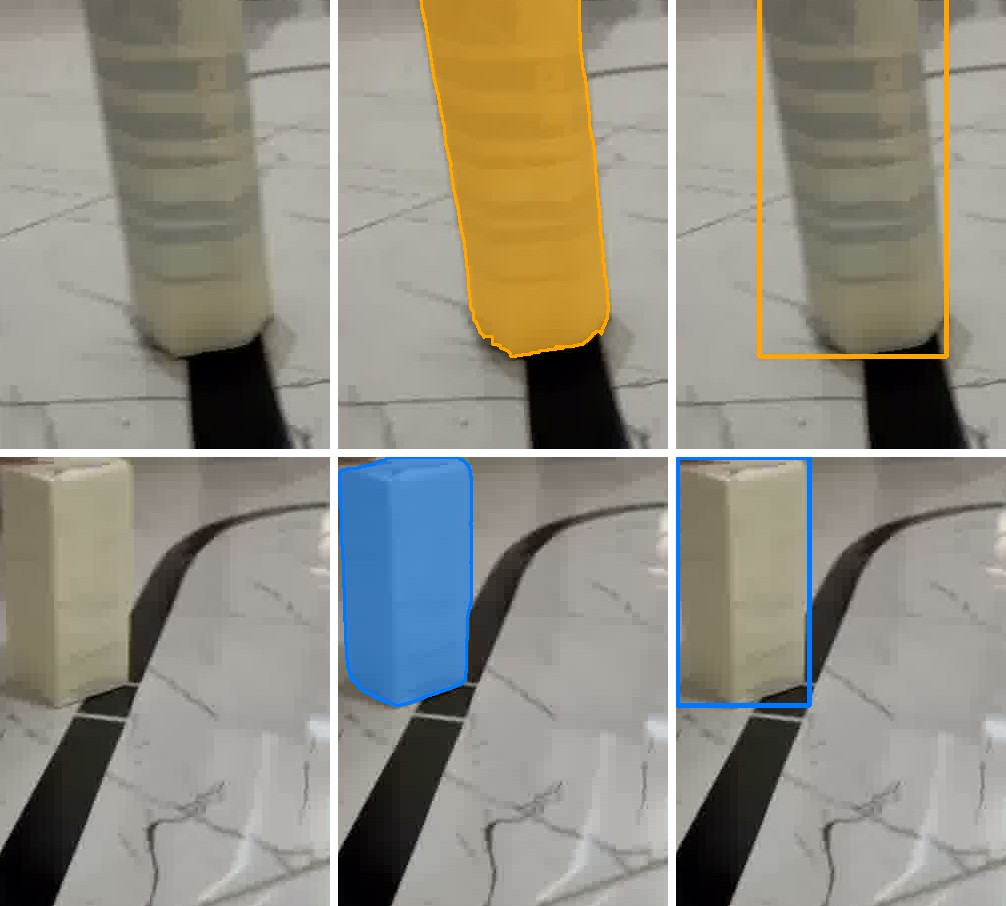
\includegraphics[width=\linewidth]{donnees/sam2_segmentation.jpg}
\caption{Image d'origine, segmentation (masque produit par SAM~2) et détection (boîte englobante déduite du
masque) pour les deux obstacles de la piste}
\label{fig:det-seg}
\end{figure}

\subsection{Application à la détection des obstacles routiers et des nids-de-poule}
Sur la route, deux familles d'obstacles doivent être reconnues. Les \textbf{usagers de la route} (piétons,
cyclistes, véhicules, animaux) sont des objets bien représentés dans les grands jeux de données publics : un
modèle préentraîné les reconnaît déjà. Les \textbf{anomalies routières} (nids-de-poule, cônes, barrières,
panneaux de chantier) sont plus spécifiques et nécessitent un apprentissage dédié. Les nids-de-poule sont les plus
difficiles : ils sont plats, de forme et de taille très variables, souvent remplis d'eau ou peu contrastés avec la
chaussée. La figure~\ref{fig:exemples-route} montre les prédictions de nos deux modèles routiers sur des images
de test.

\begin{figure}[H]
\centering
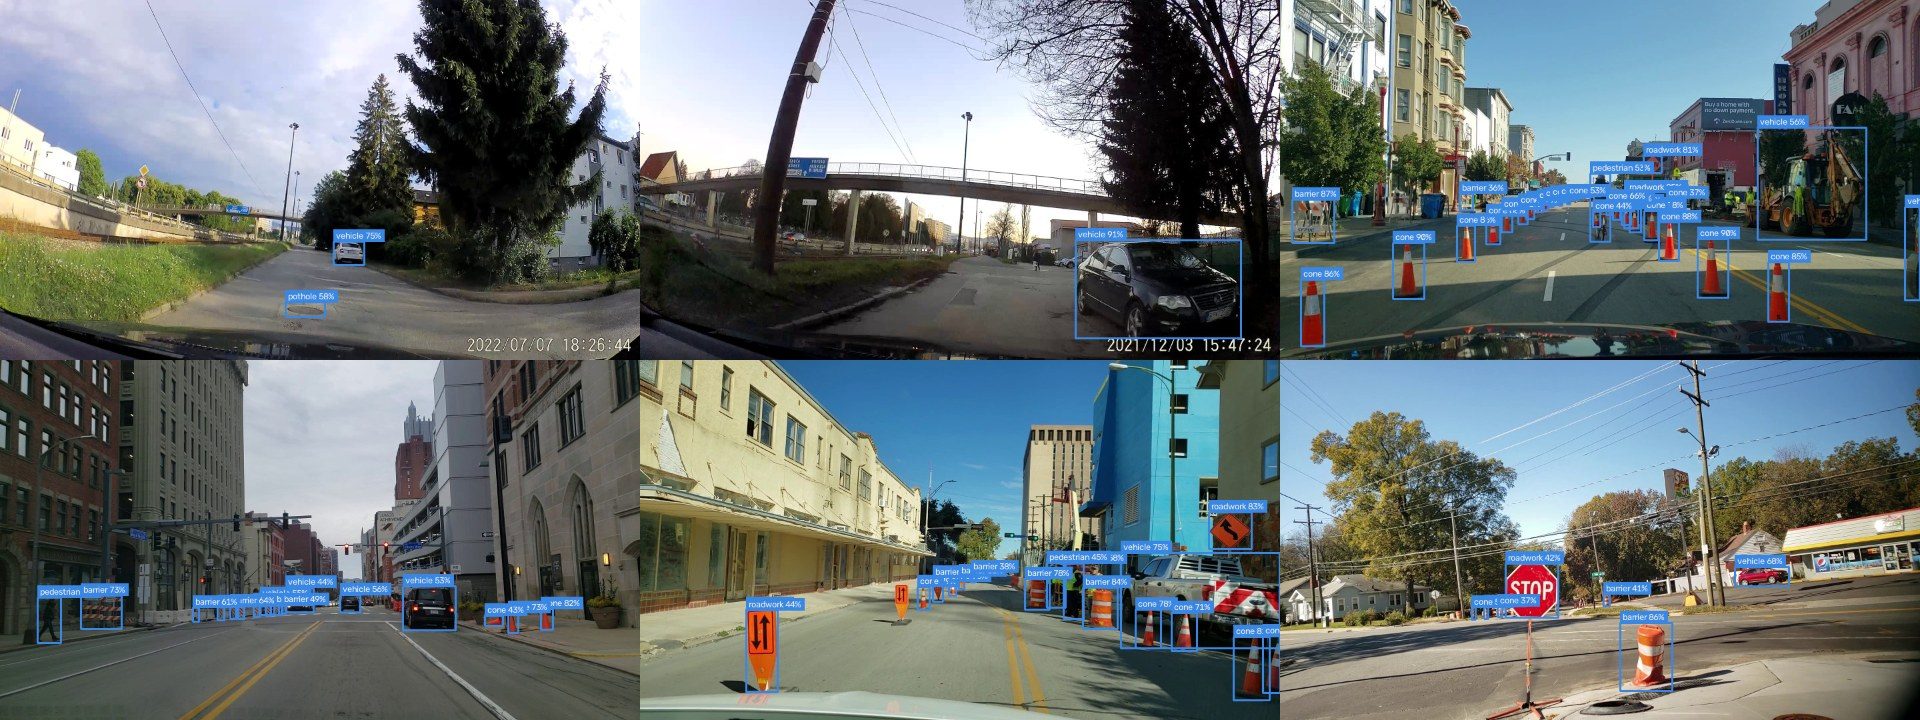
\includegraphics[width=\linewidth]{ia/reel_exemples_detection.jpg}
\caption{Détections des modèles routiers (usagers de la route et anomalies) sur des images de l'ensemble de test,
aux seuils de l'application. Les erreurs restent visibles : un nid-de-poule manqué (en haut au centre), un
panneau STOP pris pour un panneau de chantier (en bas à droite).}
\label{fig:exemples-route}
\end{figure}

% =================================================================================================
\section{Présentation des modèles YOLO26}

\subsection{Généralités sur la famille YOLO}
Les détecteurs d'objets se répartissent en deux familles. Les détecteurs \emph{à deux étapes} (R-CNN, Faster R-CNN)
proposent d'abord des régions candidates, puis les classent : ils sont précis mais lents. Les détecteurs \emph{à une
étape} prédisent directement les boîtes et les classes en une seule passe du réseau. YOLO (\textit{You Only Look
Once}), introduit par Redmon et al. en 2016~\cite{redmon2016yolo}, est le représentant le plus connu de cette
seconde famille : il découpe l'image en une grille et prédit, pour chaque cellule, des boîtes et des probabilités
de classes.

Depuis, la famille a beaucoup évolué (tableau~\ref{tab:yolo}) : ancres et prédiction multi-échelle (YOLOv3),
augmentation \textit{mosaic} (YOLOv4~\cite{bochkovskiy2020yolov4}), têtes sans ancres (YOLOv8), entraînement sans
NMS (YOLOv10~\cite{wang2024yolov10}) et, avec YOLO26, une architecture pensée pour le déploiement sur processeurs
et équipements embarqués~\cite{ultralytics26}.

\begin{table}[H]
\centering\small
\caption{Quelques étapes de l'évolution de la famille YOLO}
\label{tab:yolo}
\begin{tabular}{lll}
\toprule
\textbf{Version} & \textbf{Année} & \textbf{Apport principal} \\
\midrule
YOLO (v1)   & 2016 & Détection en une seule passe sur une grille \\
YOLOv3      & 2018 & Prédictions à trois échelles, ancres \\
YOLOv4 / v5 & 2020 & Augmentation \textit{mosaic}, écosystème PyTorch (Ultralytics) \\
YOLOv8      & 2023 & Tête sans ancres, API unifiée (détection, segmentation, pose) \\
YOLOv10     & 2024 & Affectation un-à-un : inférence sans NMS \\
YOLO11      & 2024 & Blocs C3k2 et attention C2PSA \\
YOLO26      & 2025 & Inférence de bout en bout sans NMS, suppression de la DFL, optimisé CPU / embarqué \\
\bottomrule
\end{tabular}
\end{table}

\subsection{Présentation de YOLO26 et de son architecture}
YOLO26 est la génération de détecteurs publiée par Ultralytics en 2025~\cite{ultralytics26}. Elle est déclinée en
cinq tailles : \emph{nano} (n), \emph{small} (s), \emph{medium} (m), \emph{large} (l) et \emph{extra-large} (x). Comme
ses prédécesseurs, le réseau comporte trois parties (figure~\ref{fig:yolo26}) :
\begin{itemize}
  \item un \textbf{backbone} (extracteur de caractéristiques) convolutif qui réduit progressivement la résolution
        et produit des cartes de caractéristiques à plusieurs échelles (P3, P4, P5, soit 1/8, 1/16 et 1/32 de
        l'image) ;
  \item un \textbf{neck} de type FPN/PAN~\cite{lin2017fpn,liu2018panet} qui combine ces échelles, pour détecter à la fois
        les petits objets lointains et les grands objets proches ;
  \item une \textbf{tête de détection} qui prédit, pour chaque position, la boîte et les scores de classes.
\end{itemize}
Ses principales nouveautés visent le déploiement : la tête est \textbf{de bout en bout} (affectation un-à-un) et
produit directement au plus 300 détections finales, \textbf{sans post-traitement NMS} ; la \textit{Distribution Focal
Loss} (DFL) est supprimée, ce qui simplifie l'export ; l'entraînement utilise une pondération progressive des pertes
(ProgLoss) et une affectation des étiquettes favorable aux petits objets (STAL). Exporté en ONNX, le modèle produit
un unique tenseur de sortie de taille $1 \times 300 \times 6$ : pour chaque détection, $(x_1, y_1, x_2, y_2)$, le
score et la classe. Notre modèle du prototype (YOLO26n, deux classes) compte 2,39 millions de paramètres pour
5,4 GFLOPs.

\begin{figure}[H]
\centering
\resizebox{\linewidth}{!}{%
\begin{tikzpicture}[node distance=0.3cm and 0.5cm,
  feat/.style={draw=bleufst,thick,fill=bleufst!12,minimum width=1.25cm,align=center,font=\scriptsize,rounded corners=2pt}]
  \node[bloco,minimum width=2.1cm,minimum height=2.6cm] (in) {Image\\640$\times$640$\times$3\\\scriptsize(\textit{letterbox})};
  % backbone
  \node[feat,minimum height=2.4cm,right=0.7cm of in] (b1) {Conv\\stride 2};
  \node[feat,minimum height=2.1cm,right=0.25cm of b1] (b2) {Conv\\+ C3k2};
  \node[feat,minimum height=1.8cm,right=0.25cm of b2] (b3) {C3k2\\P3/8};
  \node[feat,minimum height=1.4cm,right=0.25cm of b3] (b4) {C3k2\\P4/16};
  \node[feat,minimum height=1.05cm,right=0.25cm of b4] (b5) {SPPF\\C2PSA\\P5/32};
  \begin{scope}[on background layer]
    \node[zone,fill=bleufst!4,fit=(b1)(b5),label={[font=\bfseries\small]above:Backbone}] (bb) {};
  \end{scope}
  % neck
  \node[feat,draw=vertfst!80!black,fill=vertfst!15,minimum height=1.05cm,right=1.0cm of b5,yshift=1.25cm] (n5) {P5};
  \node[feat,draw=vertfst!80!black,fill=vertfst!15,minimum height=1.05cm,below=0.25cm of n5] (n4) {P4};
  \node[feat,draw=vertfst!80!black,fill=vertfst!15,minimum height=1.05cm,below=0.25cm of n4] (n3) {P3};
  \node[font=\scriptsize,align=center,right=0.1cm of n4] (fpn) {FPN $\downarrow$\\PAN $\uparrow$};
  \begin{scope}[on background layer]
    \node[zone,fill=vertfst!5,fit=(n5)(n3)(fpn),label={[font=\bfseries\small]above:Neck}] (nk) {};
  \end{scope}
  \draw[fleche] (b3.east) to[out=0,in=180] (n3.west);
  \draw[fleche] (b4.east) to[out=0,in=180] (n4.west);
  \draw[fleche] (b5.east) to[out=0,in=180] (n5.west);
  % head
  \node[bloc,draw=orangefst,fill=orangefst!12,minimum width=3.3cm,minimum height=2.6cm,right=0.9cm of nk]
       (head) {Tête de bout en bout\\(un-à-un, sans DFL)\\\scriptsize boîtes + classes\\\scriptsize sans NMS};
  \draw[fleche] (nk) -- (head);
  \node[bloc,minimum width=2.6cm,minimum height=2.6cm,right=0.7cm of head] (out) {Sortie\\$1 \times 300 \times 6$\\\scriptsize $x_1,y_1,x_2,y_2$,\\\scriptsize score, classe};
  \draw[fleche] (in) -- (bb); \draw[fleche] (head) -- (out);
\end{tikzpicture}}
\caption{Architecture simplifiée d'un détecteur YOLO26 : backbone, neck multi-échelle et tête de bout en bout
sans NMS}
\label{fig:yolo26}
\end{figure}

Le choix des variantes résulte d'un compromis entre précision et vitesse, l'inférence se faisant sur le processeur
de l'ordinateur : la variante \textbf{nano} pour les usagers de la route et pour le prototype, la variante
\textbf{small}, un peu plus lourde, pour les anomalies routières, plus difficiles à reconnaître.

\subsection{Utilisation des poids préentraînés sur COCO}
Entraîner un détecteur à partir de zéro demande des centaines de milliers d'images annotées. Nous utilisons
l'\textbf{apprentissage par transfert} : les modèles partent des poids publiés par Ultralytics, préentraînés sur
COCO~\cite{lin2014coco} (118\,287 images d'entraînement, 80 classes d'objets courants). Le backbone sait déjà
extraire des caractéristiques visuelles générales ; l'affinage (\textit{fine-tuning}) adapte surtout la tête aux
nouvelles classes (figure~\ref{fig:transfert}).

Pour les usagers de la route, aucun réentraînement n'est nécessaire : les classes COCO \textit{person},
\textit{bicycle}, \textit{car}, \textit{bus}, \textit{truck}, \textit{dog}, etc. sont directement regroupées en quatre
catégories utiles au véhicule (tableau~\ref{tab:classes-users}).

\begin{figure}[H]
\centering
\resizebox{0.95\linewidth}{!}{%
\begin{tikzpicture}[node distance=0.5cm and 0.8cm]
  \node[blocg,minimum width=3.2cm] (coco) {YOLO26 préentraîné\\COCO (80 classes)};
  \node[bloc,minimum width=3.4cm,above right=0.25cm and 1.2cm of coco] (u) {Usagers de la route\\\scriptsize regroupement de classes COCO};
  \node[bloco,minimum width=3.4cm,right=1.2cm of coco] (h) {Affinage sur 7\,894 images\\\scriptsize anomalies routières (YOLO26s)};
  \node[blocv,minimum width=3.4cm,below right=0.25cm and 1.2cm of coco] (t) {Affinage sur notre piste\\\scriptsize colonne / boîte (YOLO26n)};
  \draw[fleche] (coco) -- node[note,above,sloped] {sans réentraînement} (u.west);
  \draw[fleche] (coco) -- (h); \draw[fleche] (coco) -- (t.west);
  \node[bloc,minimum width=2.6cm,right=0.8cm of h] (on) {Export\\ONNX};
  \draw[fleche] (u.east) -- (on); \draw[fleche] (h) -- (on); \draw[fleche] (t.east) -- (on);
\end{tikzpicture}}
\caption{Apprentissage par transfert à partir des poids COCO}
\label{fig:transfert}
\end{figure}

\subsection{Environnement Ultralytics}
La bibliothèque Python \textbf{Ultralytics}~\cite{ultralytics26} fournit les modèles YOLO26 et toute la chaîne de
travail : chargement des jeux de données décrits par un fichier \texttt{data.yaml}, entraînement avec augmentation de
données, validation (précision, rappel, mAP, courbes et matrice de confusion), prédiction et export vers de
nombreux formats (ONNX, TensorRT, TFLite…). L'entraînement a été réalisé dans un \textbf{conteneur Docker} basé sur
l'image officielle \texttt{ultralytics/ultralytics} (Ultralytics 8.4.184, PyTorch avec CUDA), complétée par
JupyterLab, ce qui garantit un environnement identique d'une machine à l'autre. Les notebooks
\texttt{train\_road\_obstacles.ipynb} et \texttt{train\_toy\_obstacles.ipynb} s'exécutent sur ce noyau et utilisent le
GPU de l'ordinateur (NVIDIA GeForce GTX 1650 Ti, 4 Go). La figure~\ref{fig:workflow} résume le flux de travail.

\begin{figure}[H]
\centering
\resizebox{\linewidth}{!}{%
\begin{tikzpicture}[node distance=0.5cm]
  \node[bloco,minimum width=2.6cm] (d) {Données\\\scriptsize images + étiquettes};
  \node[bloc,minimum width=2.4cm,right=of d] (y) {\texttt{data.yaml}\\\scriptsize classes, splits};
  \node[blocg,minimum width=2.6cm,right=of y] (tr) {\texttt{model.train()}\\\scriptsize GPU, augmentation};
  \node[blocg,minimum width=2.6cm,right=of tr] (va) {\texttt{model.val()}\\\scriptsize test : P, R, mAP};
  \node[blocg,minimum width=2.6cm,right=of va] (ex) {\texttt{model.export()}\\\scriptsize ONNX};
  \node[blocv,minimum width=2.6cm,right=of ex] (ap) {\app\\\scriptsize ONNX Runtime};
  \foreach \a/\b in {d/y,y/tr,tr/va,va/ex,ex/ap} \draw[fleche] (\a) -- (\b);
  \begin{scope}[on background layer]
    \node[zone,fill=fond,fit=(y)(ex),label={[font=\scriptsize\bfseries]above:Notebook Jupyter — conteneur Docker Ultralytics}] {};
  \end{scope}
\end{tikzpicture}}
\caption{Flux de travail avec Ultralytics, de la préparation des données à l'intégration}
\label{fig:workflow}
\end{figure}

\subsection{Adaptation du modèle aux besoins du projet}
Les besoins du projet ont conduit à trois modèles complémentaires (tableau~\ref{tab:modeles}). En environnement
réel, deux modèles s'exécutent en parallèle sur chaque image et leurs détections sont fusionnées : l'un apporte la
connaissance générale de COCO sur les usagers de la route, l'autre la connaissance spécialisée des anomalies. Pour le
prototype, un modèle nano dédié reconnaît les deux obstacles de la piste. Les classes de chaque modèle sont
traduites vers un vocabulaire commun à l'application (\texttt{pedestrian}, \texttt{vehicle}, \texttt{pothole},
\texttt{cone}, \texttt{box}…), auquel sont associés les poids de danger utilisés pour la gravité.

\begin{table}[H]
\centering\small
\caption{Les trois modèles du projet}
\label{tab:modeles}
\begin{tabularx}{\linewidth}{l l l X}
\toprule
\textbf{Modèle} & \textbf{Variante} & \textbf{Entraînement} & \textbf{Classes détectées} \\
\midrule
Usagers de la route & YOLO26n & préentraîné COCO & piéton, cycliste, véhicule, animal \\
Anomalies routières & YOLO26s & affiné 8 h, 36 époques & nid-de-poule, cône, barrière, panneau de chantier \\
Obstacles du prototype & YOLO26n & affiné 30 min, 73 époques & colonne, boîte \\
\bottomrule
\end{tabularx}
\end{table}

% =================================================================================================
\section{Préparation des données}

\subsection{Présentation des données réelles}
Le modèle d'anomalies routières a été entraîné sur la réunion de deux jeux de données publics d'images de caméras
embarquées :
\begin{itemize}
  \item \textbf{Potholes under challenging conditions}~\cite{bucko2022potholes} (Bučko et al., \textit{Sensors},
        2022, licence CC BY 4.0) : des images de nids-de-poule extraites de vidéos de conduite en Slovaquie, dans
        des conditions difficiles (pluie, ombres, nuit, chaussée mouillée) ;
  \item \textbf{ROADWork}~\cite{ghosh2025roadwork} (Ghosh et al., ICCV 2025, Carnegie Mellon University, licence
        ODC-By 1.0) : des images de zones de travaux dans plusieurs villes, avec des cônes, des barrières et des
        panneaux de signalisation temporaire.
\end{itemize}
Au total, \textbf{7\,894 images} réelles ont été retenues. Les annotations d'origine ont été converties au format
YOLO et leurs nombreuses sous-catégories regroupées en quatre classes. La figure~\ref{fig:donnees-reelles} montre
des images d'entraînement et la répartition des étiquettes.

\begin{figure}[H]
\centering
\begin{subfigure}[b]{0.52\linewidth}\centering
  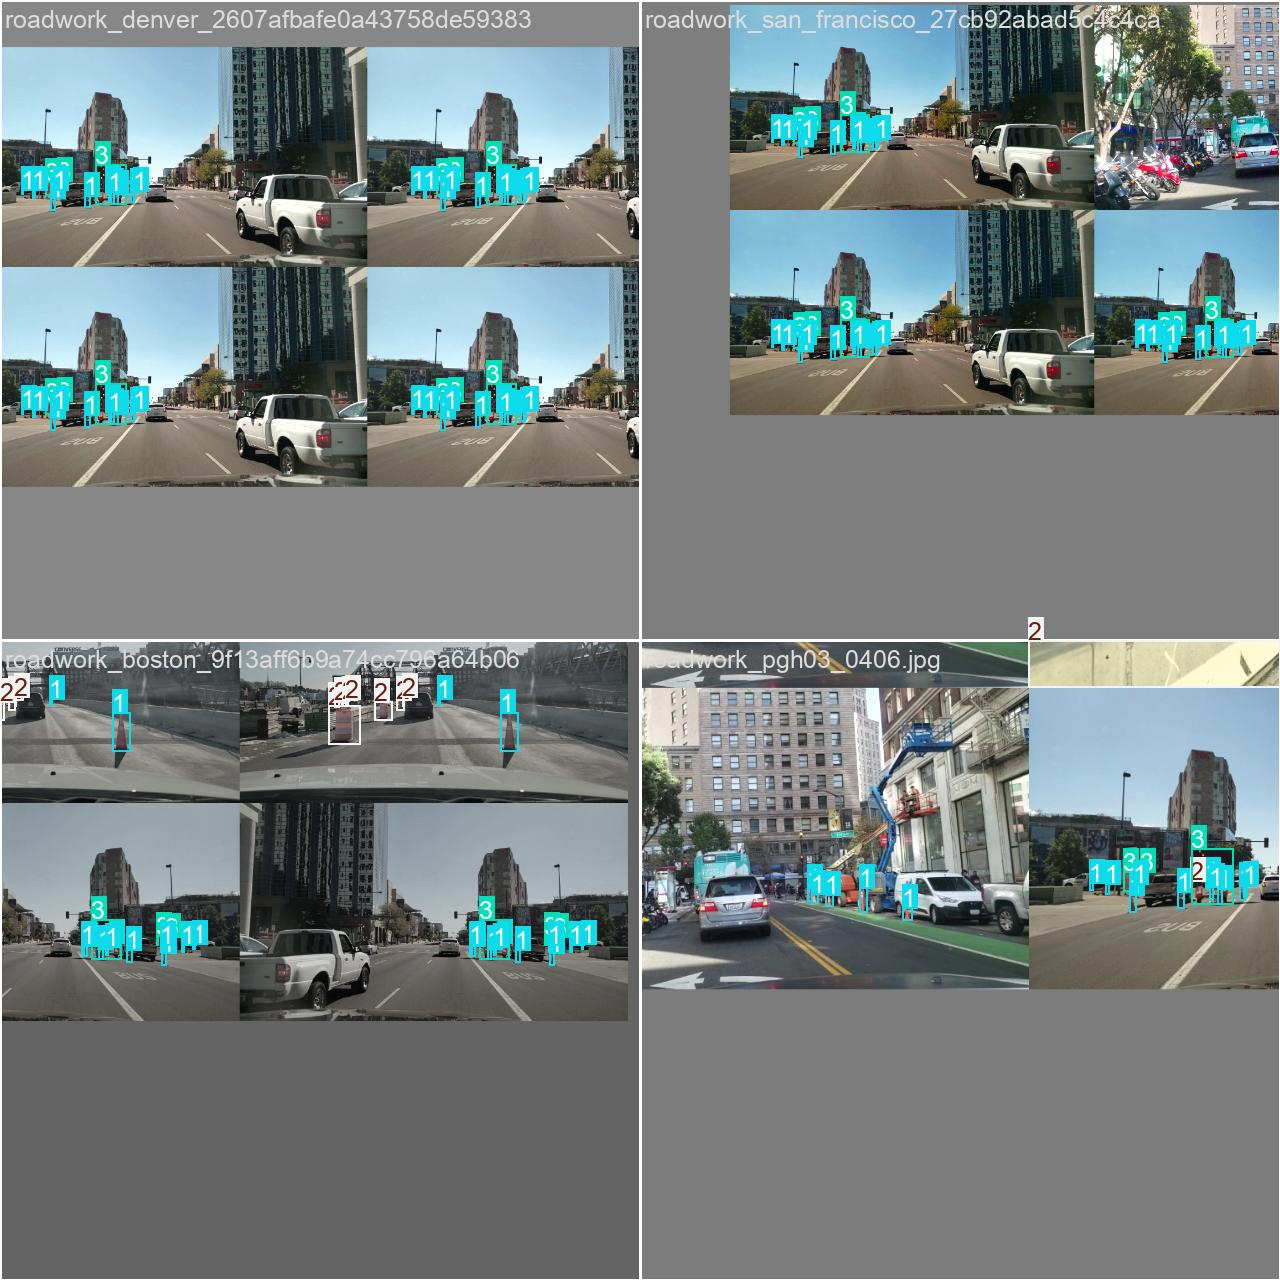
\includegraphics[width=\linewidth]{ia/reel_train_batch.jpg}
  \caption{Lot d'entraînement (mosaïques augmentées)}
\end{subfigure}\hfill
\begin{subfigure}[b]{0.45\linewidth}\centering
  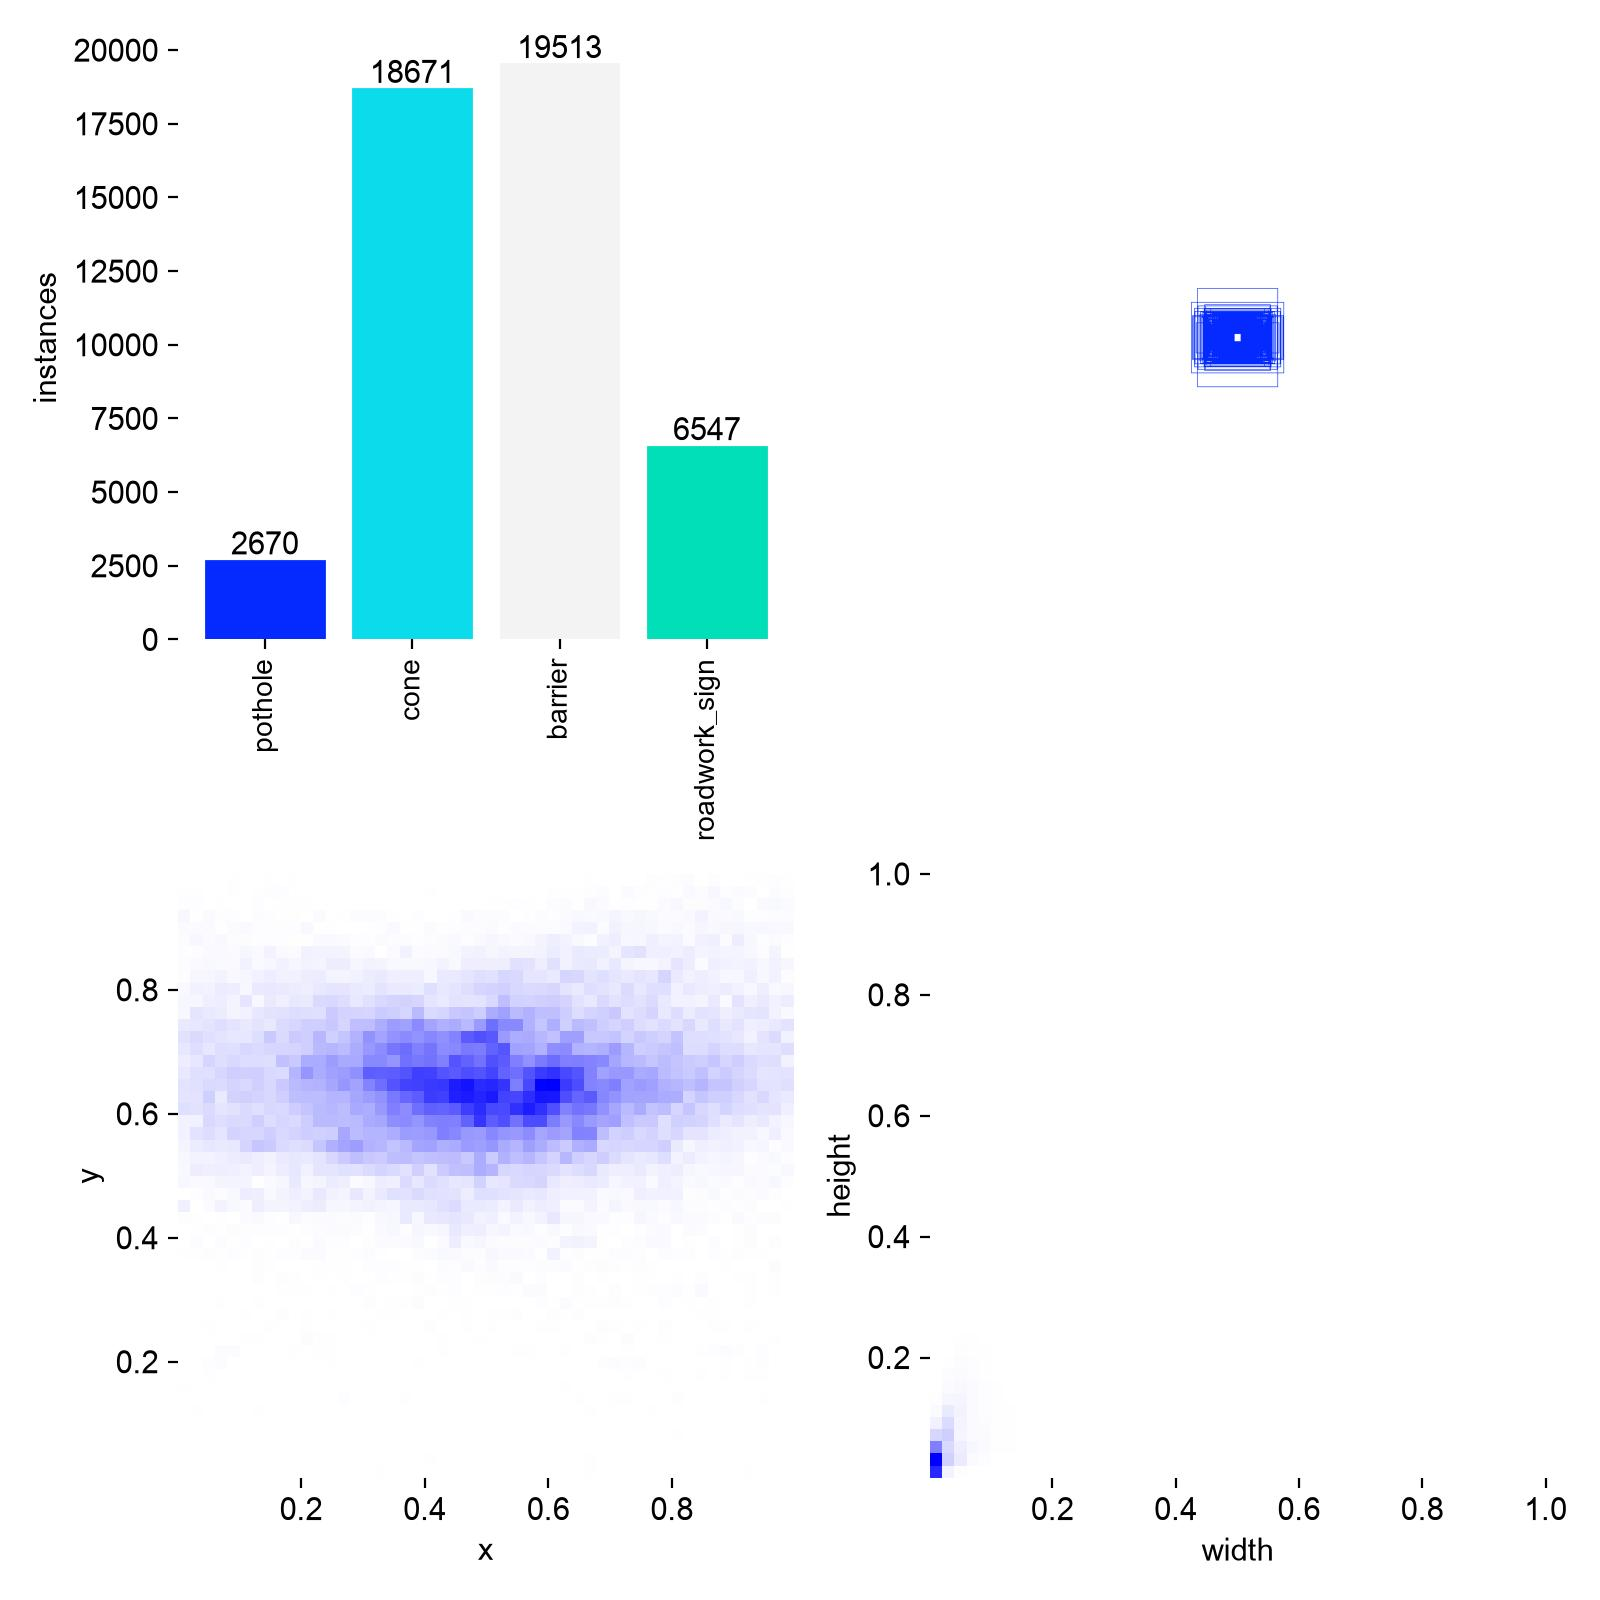
\includegraphics[width=\linewidth]{ia/reel_labels.jpg}
  \caption{Statistiques des étiquettes}
\end{subfigure}
\caption{Données réelles : exemples d'images d'entraînement et distribution des annotations}
\label{fig:donnees-reelles}
\end{figure}

Les vidéos qui alimentent la caméra embarquée de CAR-01 dans l'application proviennent de sources libres
(Wikimedia Commons, licences CC BY, CC BY-SA ou domaine public) et des images de test du jeu Potholes : elles ne
servent qu'à la démonstration, jamais à l'entraînement.

\subsection{Présentation des données du prototype}
Aucun jeu de données public ne contient notre piste et nos obstacles. Nous avons donc constitué le nôtre : une
vidéo filmée à hauteur de voiture en suivant le ruban, dont nous avons extrait \textbf{249 images}
(832\,$\times$\,464 pixels). La vidéo contient des passages devant la colonne, devant la boîte (sous plusieurs
faces, dont celle portant le logo) et des portions de piste vide (figure~\ref{fig:donnees-proto}). Une photo de la
piste vue de dessus et une photo de chaque obstacle ont complété ces images pour définir précisément les classes.

\begin{figure}[H]
\centering
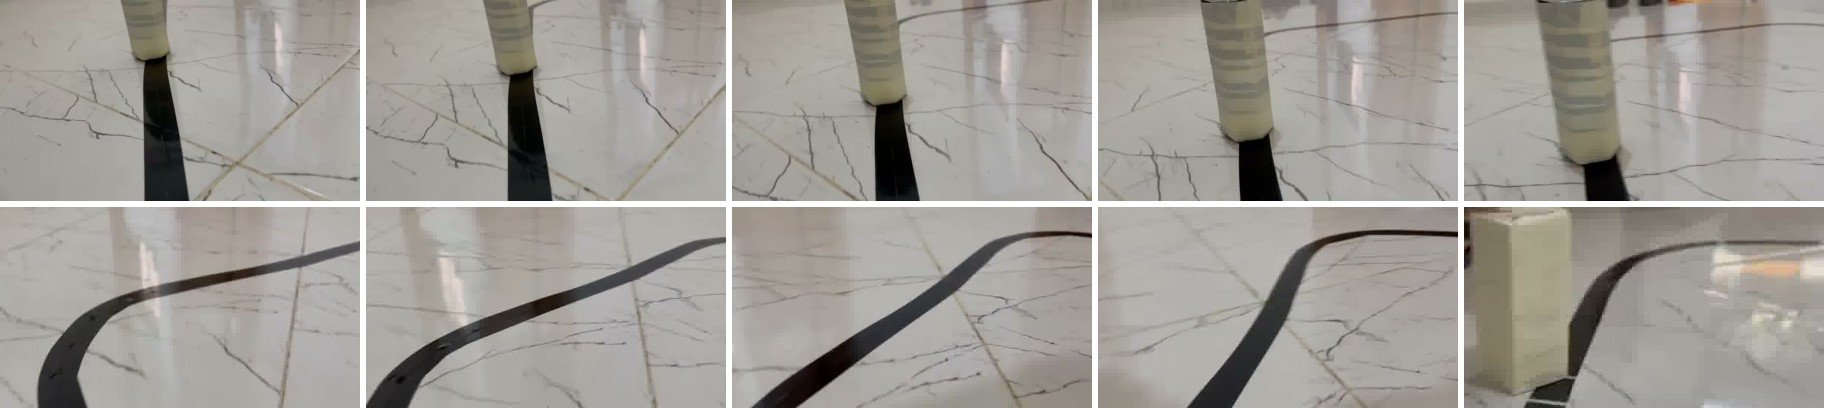
\includegraphics[width=\linewidth]{donnees/toy_frames.jpg}
\caption{Données du prototype : images extraites de la vidéo (passage devant la colonne, piste vide, boîte)}
\label{fig:donnees-proto}
\end{figure}

\subsection{Organisation et annotation des images}
Les deux jeux de données suivent l'organisation standard d'Ultralytics : un dossier \texttt{images/} et un dossier
\texttt{labels/}, chacun divisé en \texttt{train}, \texttt{val} et \texttt{test}. Chaque image possède un fichier texte
contenant une ligne par objet :
\begin{center}
\texttt{<classe> <x\_centre> <y\_centre> <largeur> <hauteur>}
\end{center}
où les coordonnées sont normalisées entre 0 et 1. Une image sans objet a un fichier vide : elle sert d'exemple
négatif (« rien à détecter ici »).

Pour les données du prototype, l'annotation manuelle de chaque image aurait été longue. Nous avons utilisé le
\textbf{suivi vidéo de SAM~2} (\textit{Segment Anything Model 2})~\cite{ravi2024sam2} : pour chaque séquence où un
obstacle est visible, un seul clic sur l'obstacle dans une image de référence suffit ; SAM~2 propage ensuite le
masque dans toute la séquence, en avant et en arrière (figure~\ref{fig:sam2}). Un filtre élimine les pixels très
sombres pour ne pas inclure le ruban noir sous la colonne. Les boîtes sont déduites des masques et \textbf{toutes ont
été vérifiées visuellement} sur des planches de contrôle. On obtient 248 images annotées (une image floue a été
écartée) contenant 141 boîtes.

\begin{figure}[H]
\centering
\resizebox{\linewidth}{!}{%
\begin{tikzpicture}[node distance=0.5cm]
  \node[bloco,minimum width=2.6cm] (v) {Vidéo\\\scriptsize 249 images};
  \node[bloc,minimum width=2.8cm,right=of v] (c) {1 clic par séquence\\\scriptsize image de référence};
  \node[blocg,minimum width=2.8cm,right=of c] (s) {Suivi SAM~2\\\scriptsize masques sur la séquence};
  \node[bloc,minimum width=2.6cm,right=of s] (f) {Filtre\\\scriptsize pixels du ruban};
  \node[bloc,minimum width=2.6cm,right=of f] (b) {Boîtes YOLO\\\scriptsize + masques};
  \node[blocv,minimum width=2.6cm,right=of b] (r) {Vérification\\\scriptsize planches visuelles};
  \foreach \x/\y in {v/c,c/s,s/f,f/b,b/r} \draw[fleche] (\x) -- (\y);
\end{tikzpicture}}

\vspace{0.3cm}
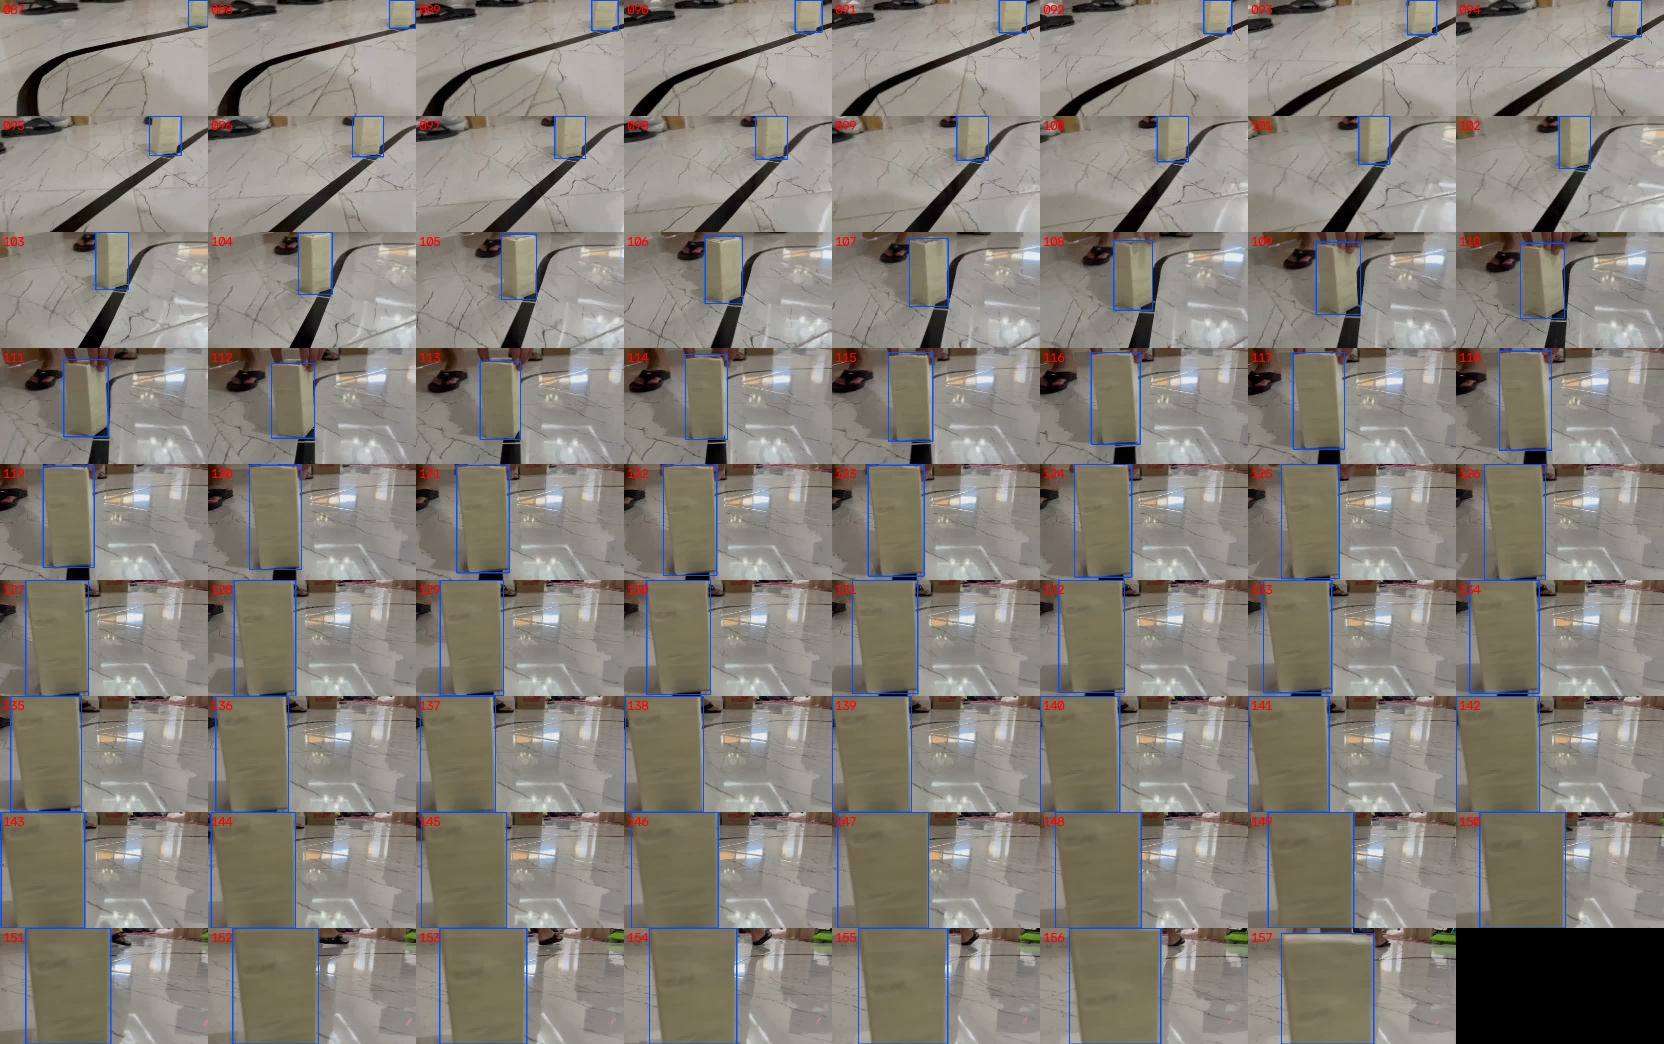
\includegraphics[width=0.95\linewidth]{donnees/toy_sam2_suivi.jpg}
\caption{Annotation automatique par suivi vidéo avec SAM~2 : chaîne de traitement et planche de contrôle d'une
séquence de la boîte}
\label{fig:sam2}
\end{figure}

\subsection{Définition des classes à reconnaître}
Les classes ont été définies en fonction de l'usage : chacune doit correspondre à une réaction différente du
véhicule ou à un niveau de danger différent (tableaux~\ref{tab:classes-users} et~\ref{tab:classes-hazards}).

\begin{table}[H]
\centering\small
\caption{Classes du modèle des usagers de la route (regroupement des classes COCO)}
\label{tab:classes-users}
\begin{tabular}{ll}
\toprule
\textbf{Classe de l'application} & \textbf{Classes COCO regroupées} \\
\midrule
\texttt{pedestrian} (piéton) & person \\
\texttt{cyclist} (cycliste) & bicycle \\
\texttt{vehicle} (véhicule) & car, motorcycle, bus, truck, train \\
\texttt{animal} & dog, cat, horse, cow, sheep, bird \\
\bottomrule
\end{tabular}
\end{table}

\begin{table}[H]
\centering\small
\caption{Classes des modèles entraînés}
\label{tab:classes-hazards}
\begin{tabularx}{\linewidth}{l l X}
\toprule
\textbf{Modèle} & \textbf{Classe} & \textbf{Contenu} \\
\midrule
Anomalies & \texttt{pothole} & nids-de-poule \\
          & \texttt{cone} & cônes et balises tubulaires \\
          & \texttt{barrier} & fûts, barricades, barrières, clôtures, panneaux verticaux \\
          & \texttt{roadwork\_sign} & panneaux de chantier, flèches lumineuses, panneaux à messages \\
\midrule
Prototype & \texttt{column} & colonne rayée à sommet noir \\
          & \texttt{box} & boîte de couleur crème (logo rouge sur une face) \\
\bottomrule
\end{tabularx}
\end{table}

\subsection{Prétraitement et augmentation des données}
Toutes les images sont redimensionnées en conservant leurs proportions et complétées par des bandes
(\textit{letterbox}) jusqu'à la taille d'entrée du réseau : 640\,$\times$\,640 pour le modèle routier,
320\,$\times$\,320 pour le prototype, résolution proche de celle de l'ESP32-CAM.

Pendant l'entraînement, Ultralytics applique des augmentations aléatoires qui multiplient la variété des
exemples : assemblage de quatre images en mosaïque (désactivé pendant les 10 dernières époques), variations de
teinte, de saturation et de luminosité, translations, changements d'échelle ($\pm 50\,\%$) et symétries
horizontales.

Pour le prototype, deux augmentations spécifiques ont été développées :
\begin{itemize}
  \item \textbf{l'aspect ESP32-CAM} : la vidéo a été filmée avec un téléphone en 16:9, alors que l'ESP32-CAM
        fournit des images 4:3 de moindre qualité. 60\,\% des images d'entraînement sont donc converties en images
        « style ESP32-CAM » : recadrage aléatoire au format 4:3, réduction à 320\,$\times$\,240, flou, dominante de
        couleur, bruit et forte compression JPEG ; les boîtes sont recalculées et un obstacle coupé à plus de 60\,\%
        par le recadrage est écarté (figure~\ref{fig:augmentation}a) ;
  \item \textbf{le copier-coller}~\cite{ghiasi2021copypaste} : les obstacles, découpés grâce à leur masque SAM~2, sont
        collés sur des images de piste vide, à de nouvelles positions et distances (plus grands lorsqu'ils sont
        proches de la caméra), avec ajustement de la luminosité. 400 images supplémentaires sont ainsi créées, avec des
        boîtes exactes (figure~\ref{fig:augmentation}b).
\end{itemize}

\begin{figure}[H]
\centering
\begin{subfigure}[b]{0.49\linewidth}\centering
  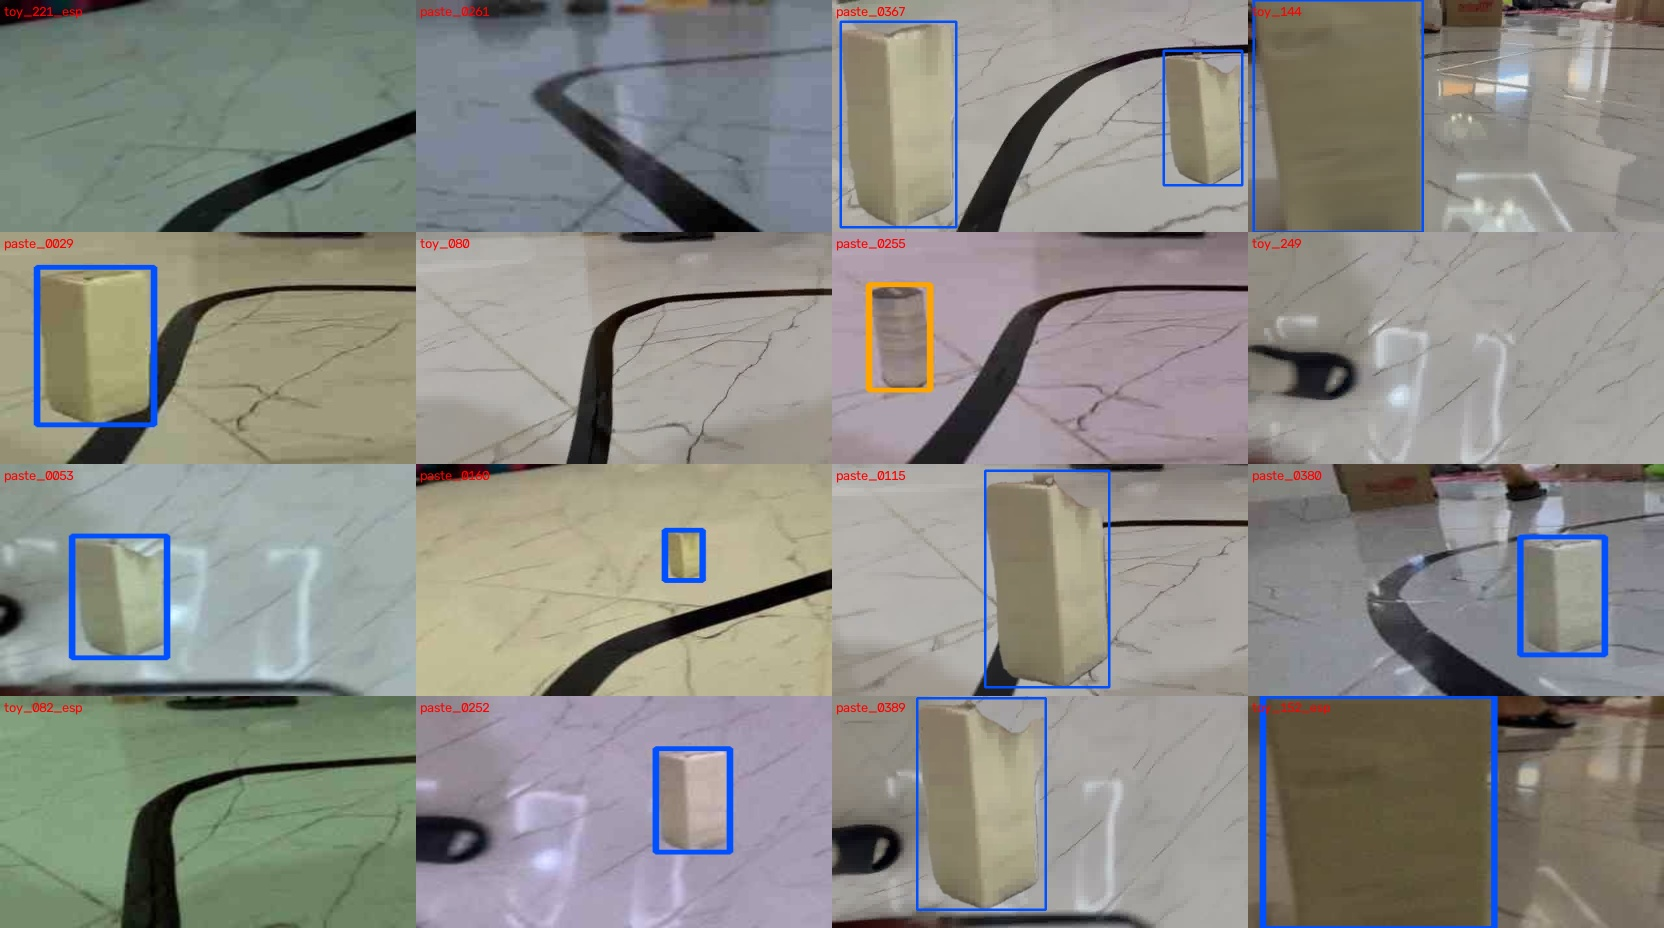
\includegraphics[width=\linewidth]{donnees/toy_esp32_look.jpg}
  \caption{Images converties au style ESP32-CAM}
\end{subfigure}\hfill
\begin{subfigure}[b]{0.49\linewidth}\centering
  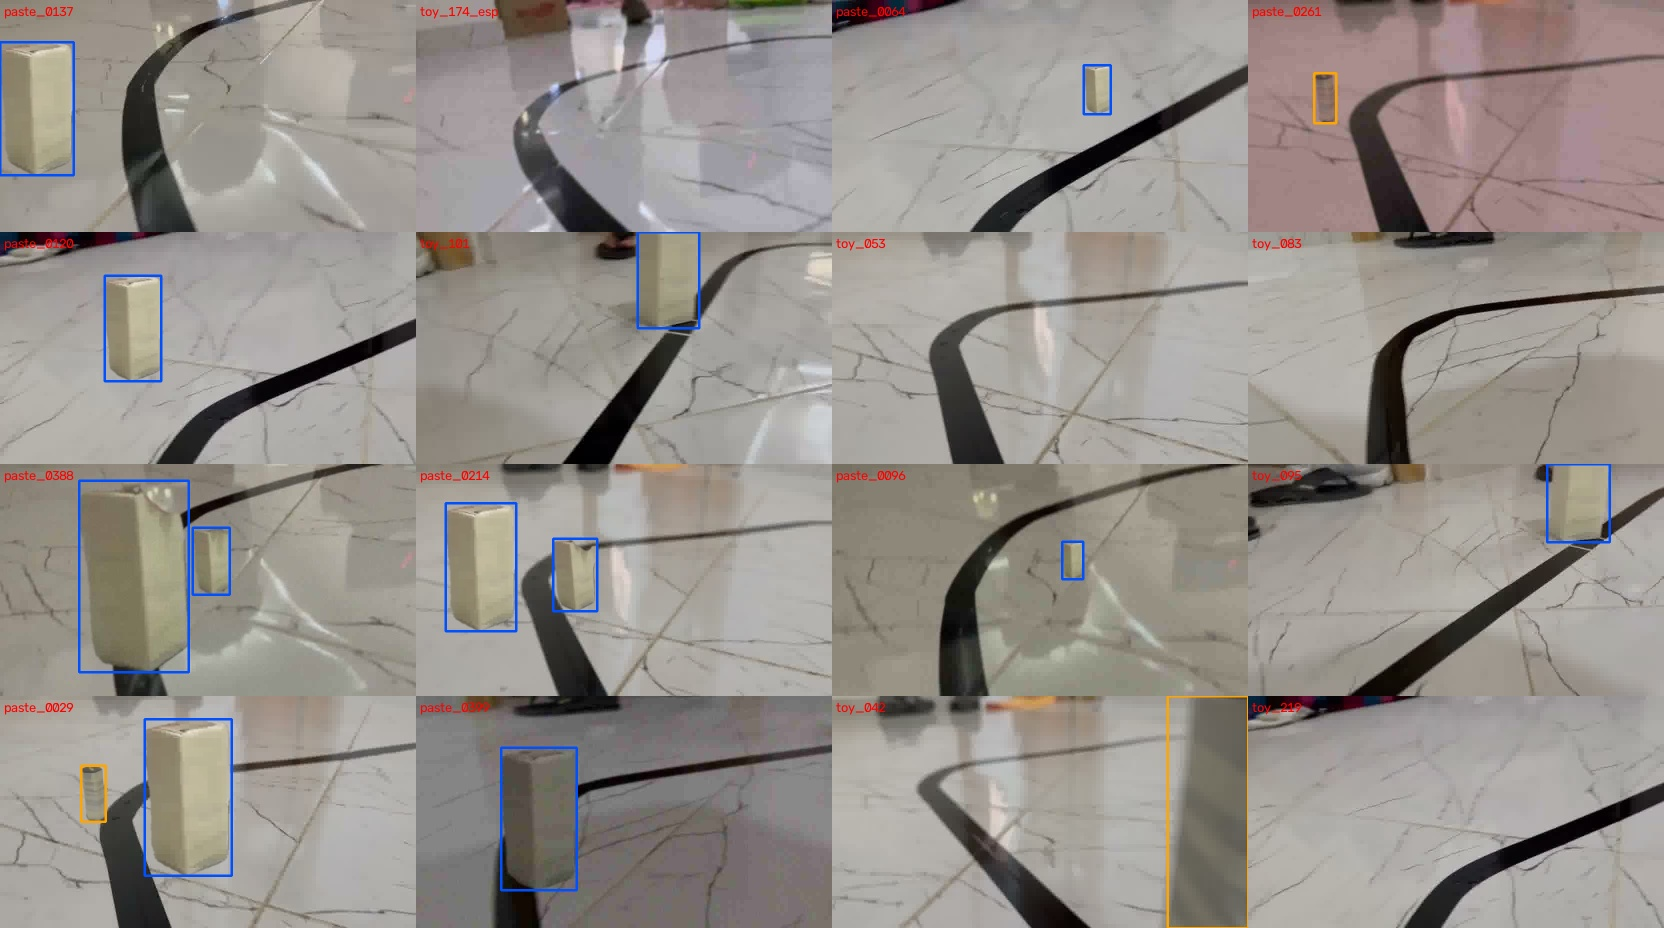
\includegraphics[width=\linewidth]{donnees/toy_train_images.jpg}
  \caption{Images d'entraînement, dont copier-coller}
\end{subfigure}
\caption{Augmentations spécifiques au prototype}
\label{fig:augmentation}
\end{figure}

\subsection{Division des données en ensembles d'entraînement, de validation et de test}
Les données sont réparties en trois ensembles : l'\textbf{entraînement} sert à ajuster les poids, la
\textbf{validation} à suivre l'apprentissage et à choisir les réglages, et le \textbf{test}, jamais utilisé avant
l'évaluation finale, à mesurer les performances.

Une précaution est essentielle avec des images extraites de vidéos : deux images voisines sont presque
identiques. Une répartition aléatoire placerait des quasi-doublons à la fois en entraînement et en test et
gonflerait artificiellement les résultats. Nous avons donc découpé \textbf{dans le temps} :
\begin{itemize}
  \item pour les nids-de-poule, chaque trajet est divisé en 80\,/\,10\,/\,10\,\% avec un intervalle de séparation ;
        pour ROADWork, la répartition géographique officielle est conservée (validation et test proviennent de lieux
        absents de l'entraînement) ;
  \item pour le prototype, chaque séquence de la vidéo est découpée en blocs temporels : un bloc pour la
        validation, un autre pour le test, le reste pour l'entraînement, avec des images d'intervalle exclues
        (figure~\ref{fig:split}).
\end{itemize}

\begin{figure}[H]
\centering
\begin{tikzpicture}[x=1.45cm,y=1cm]
  \foreach \a/\b/\c/\t in {0/3.4/bleufst/Entraînement,3.8/4.8/orangefst/Validation,5.2/6.2/vertfst!80!black/Test,
                           6.6/10/bleufst/Entraînement}
    {\fill[\c!35,draw=\c] (\a,0) rectangle (\b,0.6); \node[font=\scriptsize] at ({(\a+\b)/2},0.3) {\t};}
  \foreach \a/\b in {3.4/3.8,4.8/5.2,6.2/6.6} \filldraw[fill=gris!25,draw=gris] (\a,0) rectangle (\b,0.6);
  \draw[fleche] (0,-0.25) -- (10.2,-0.25) node[right,font=\scriptsize] {temps};
  \node[font=\scriptsize,gris] at (5,-0.6) {(intervalles gris : images exclues, pour séparer les ensembles)};
\end{tikzpicture}
\caption{Découpage temporel d'une séquence vidéo du prototype}
\label{fig:split}
\end{figure}

\begin{table}[H]
\centering\small
\caption{Répartition des données}
\label{tab:split}
\begin{tabular}{lrrr}
\toprule
\textbf{Ensemble} & \textbf{Entraînement} & \textbf{Validation} & \textbf{Test} \\
\midrule
Anomalies routières (images réelles) & 6\,324 & 755 & 815 \\
\quad objets annotés dans le test & & & 5\,105 \\
Prototype — images réelles de la vidéo & 169 & 26 & 26 \\
\quad + images style ESP32-CAM & 96 & — & 26 \\
\quad + images par copier-coller & 400 & — & — \\
\bottomrule
\end{tabular}
\end{table}

Le test du prototype comprend 26 images réelles (15 obstacles, 11 images de piste vide) et leurs 26 équivalents
convertis au style ESP32-CAM 320\,$\times$\,240, qui constituent un second ensemble de test plus proche des
conditions réelles.

% =================================================================================================
\section{Développement des deux modèles}

\subsection{Modèle destiné aux données réelles}
Le modèle d'anomalies routières est un YOLO26s affiné à partir des poids COCO sur les 6\,324 images
d'entraînement. Il est associé au modèle COCO des usagers de la route : les deux sont décrits dans un \emph{profil}
(\texttt{models/real\_road.json}) qui indique, pour chacun, le fichier ONNX, la taille d'entrée, le seuil de
confiance et la correspondance des classes. Les deux modèles s'exécutent en parallèle sur chaque image de la
caméra embarquée.

\subsection{Modèle destiné au prototype}
Le modèle du prototype est un YOLO26n affiné sur les 665 images d'entraînement (169 réelles, 96 au style
ESP32-CAM et 400 par copier-coller). La variante nano et l'entrée 320\,$\times$\,320 permettent une analyse en
temps réel du flux de la caméra sur le processeur. Son profil (\texttt{models/proto\_toy.json}) est chargé
automatiquement lorsque l'application est en mode Prototype.

\subsection{Configuration des modèles et des poids préentraînés}
Le tableau~\ref{tab:hyper} résume la configuration d'entraînement. La carte graphique (GTX 1650 Ti, 4 Go) a imposé
deux adaptations : la précision mixte (AMP) étant instable sur ce modèle de GPU, Ultralytics l'a désactivée et
l'entraînement s'est fait en 32 bits ; la taille de lot a été réduite à 4 images pour le modèle \emph{small} afin
de tenir dans la mémoire. Pour le modèle routier, la durée a été fixée par un budget de temps de 8 heures (paramètre
\texttt{time}) plutôt que par un nombre d'époques.

\begin{table}[H]
\centering\small
\caption{Configuration d'entraînement des deux modèles}
\label{tab:hyper}
\begin{tabular}{lll}
\toprule
\textbf{Paramètre} & \textbf{Anomalies routières} & \textbf{Prototype} \\
\midrule
Modèle de départ & \texttt{yolo26s.pt} (COCO) & \texttt{yolo26n.pt} (COCO) \\
Taille d'entrée & 640\,$\times$\,640 & 320\,$\times$\,320 \\
Taille de lot & 4 & 16 \\
Durée & budget de 8 h (36 époques) & 80 époques max. (arrêt à 73) \\
Arrêt anticipé (\textit{patience}) & 100 époques & 30 époques \\
Taux d'apprentissage & 0,01, décroissance en cosinus & 0,01, décroissance en cosinus \\
Mosaïque & oui, désactivée les 10 dernières époques & idem \\
Précision de calcul & FP32 (AMP désactivée) & FP32 \\
Matériel & GTX 1650 Ti (4 Go) & GTX 1650 Ti (4 Go) \\
Durée réelle & 8,0 h & 30 min \\
\bottomrule
\end{tabular}
\end{table}

\subsection{Procédure d'entraînement et de validation}
À chaque époque, le modèle parcourt l'ensemble d'entraînement par lots ; pour chaque lot, il calcule une fonction
de perte qui combine une perte de localisation (écart entre boîtes prédites et réelles, à base d'IoU) et une perte
de classification, puis met à jour ses poids par descente de gradient. À la fin de chaque époque, il est évalué sur
l'ensemble de validation et les meilleurs poids sont conservés (\texttt{best.pt}). Les notebooks affichent la
progression en temps réel ; un notebook de suivi (\texttt{monitor\_training.ipynb}) permet de consulter les courbes
pendant un entraînement de longue durée.

La figure~\ref{fig:courbes} présente les courbes d'apprentissage des deux modèles. Pour le modèle routier, les
pertes diminuent régulièrement et le mAP de validation progresse encore à la fin du budget de 8 heures, ce qui
indique qu'un entraînement plus long améliorerait encore le modèle. Pour le prototype, les métriques de validation
atteignent rapidement leur maximum et l'arrêt anticipé intervient à la 73\textsuperscript{e} époque.

\begin{figure}[H]
\centering
\begin{subfigure}[b]{\linewidth}\centering
  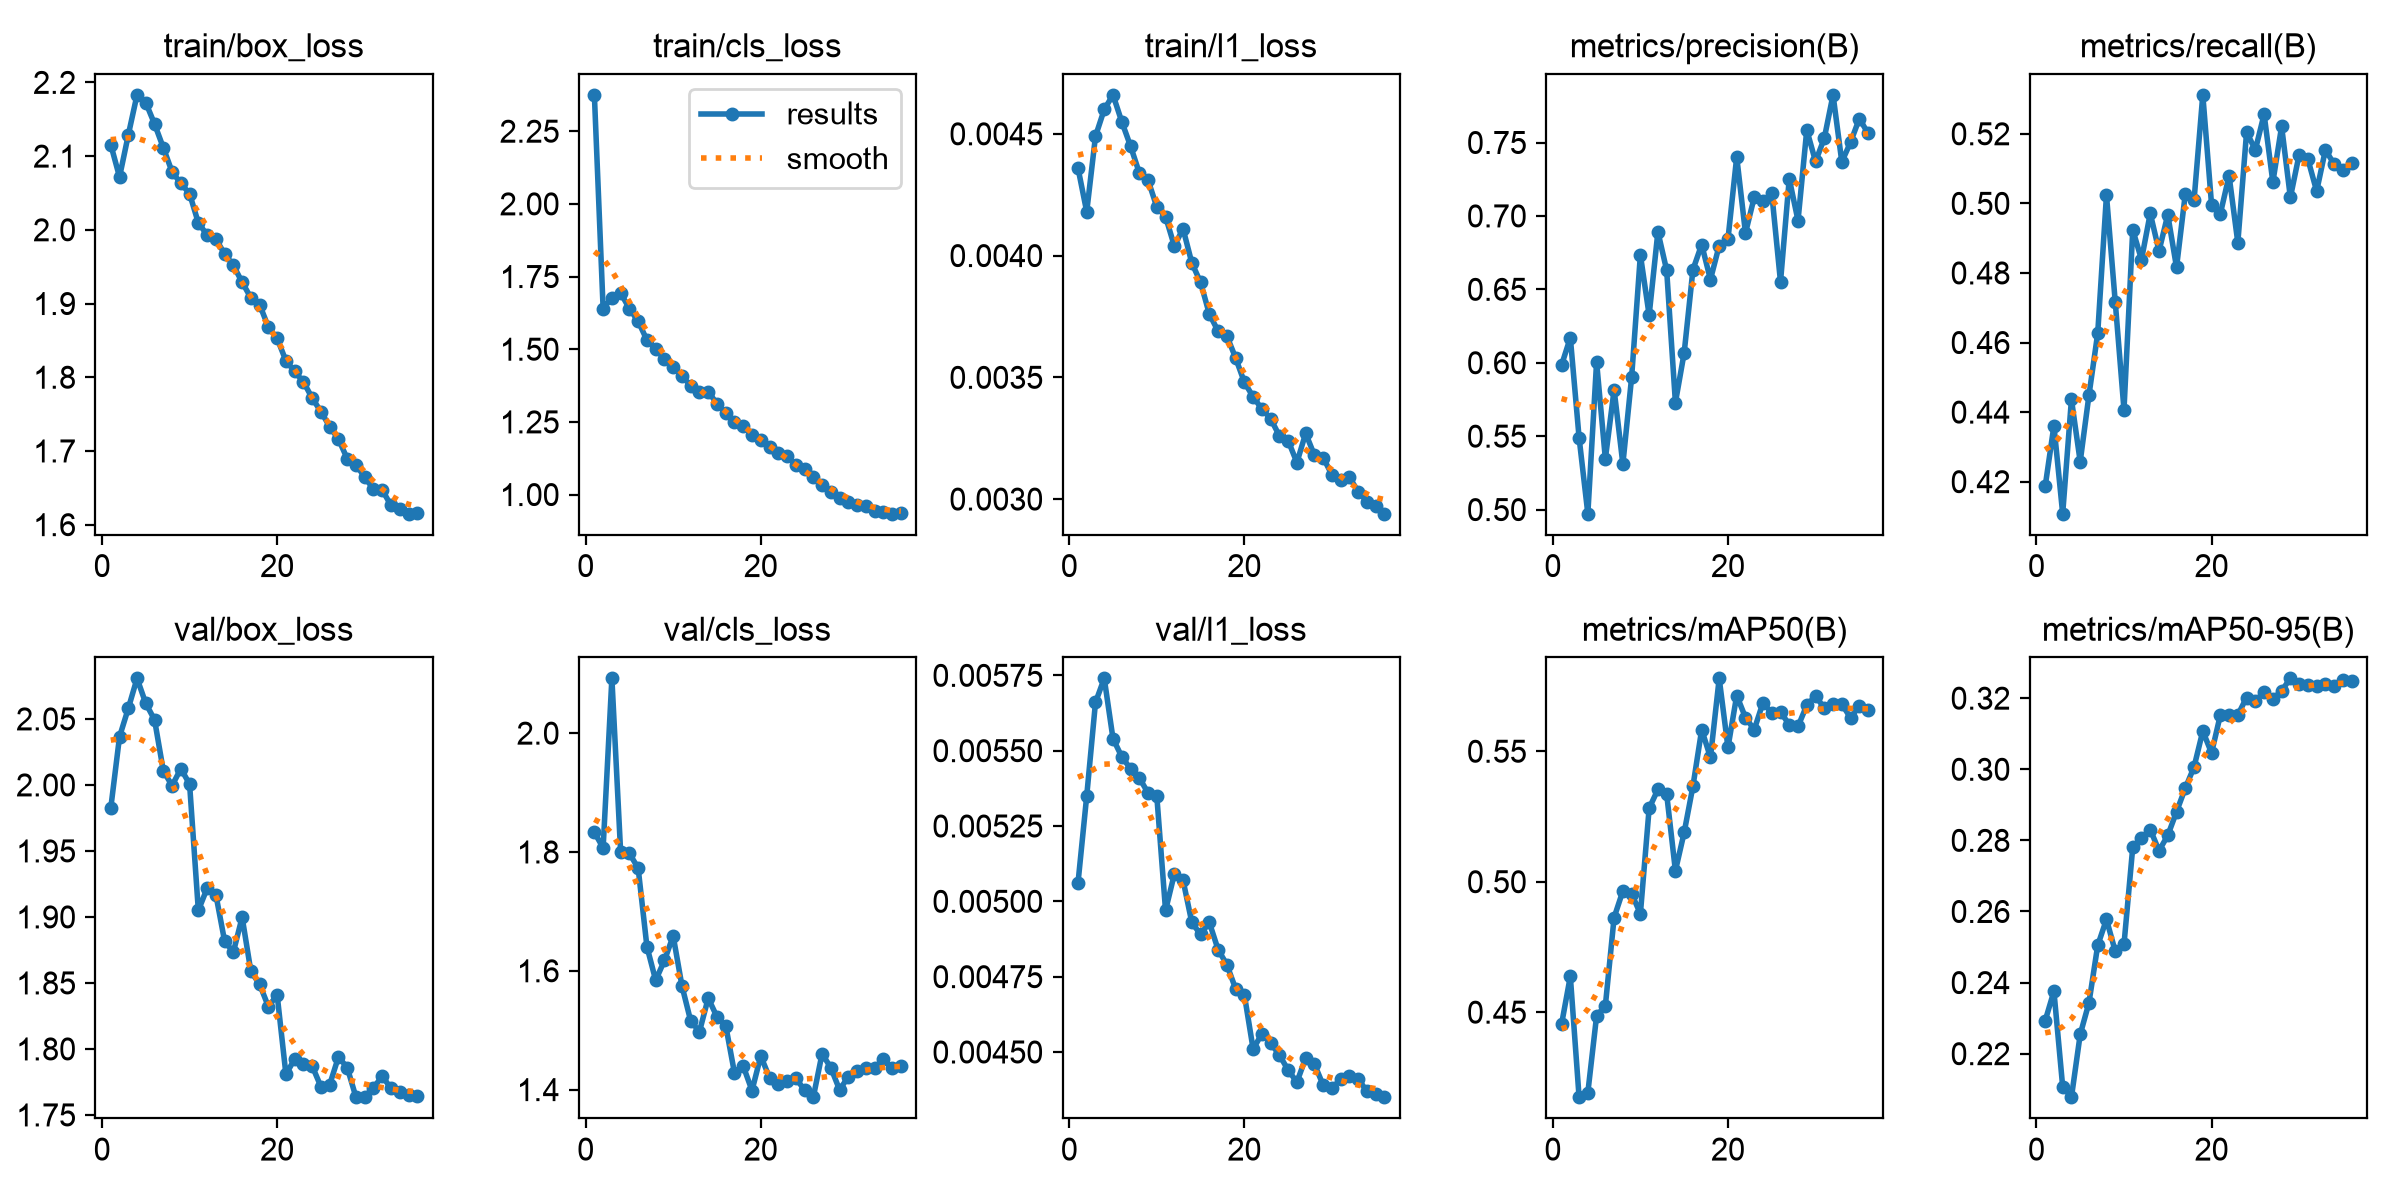
\includegraphics[width=0.9\linewidth]{ia/reel_results.png}
  \caption{Modèle d'anomalies routières (YOLO26s, 36 époques)}
\end{subfigure}

\vspace{0.2cm}
\begin{subfigure}[b]{\linewidth}\centering
  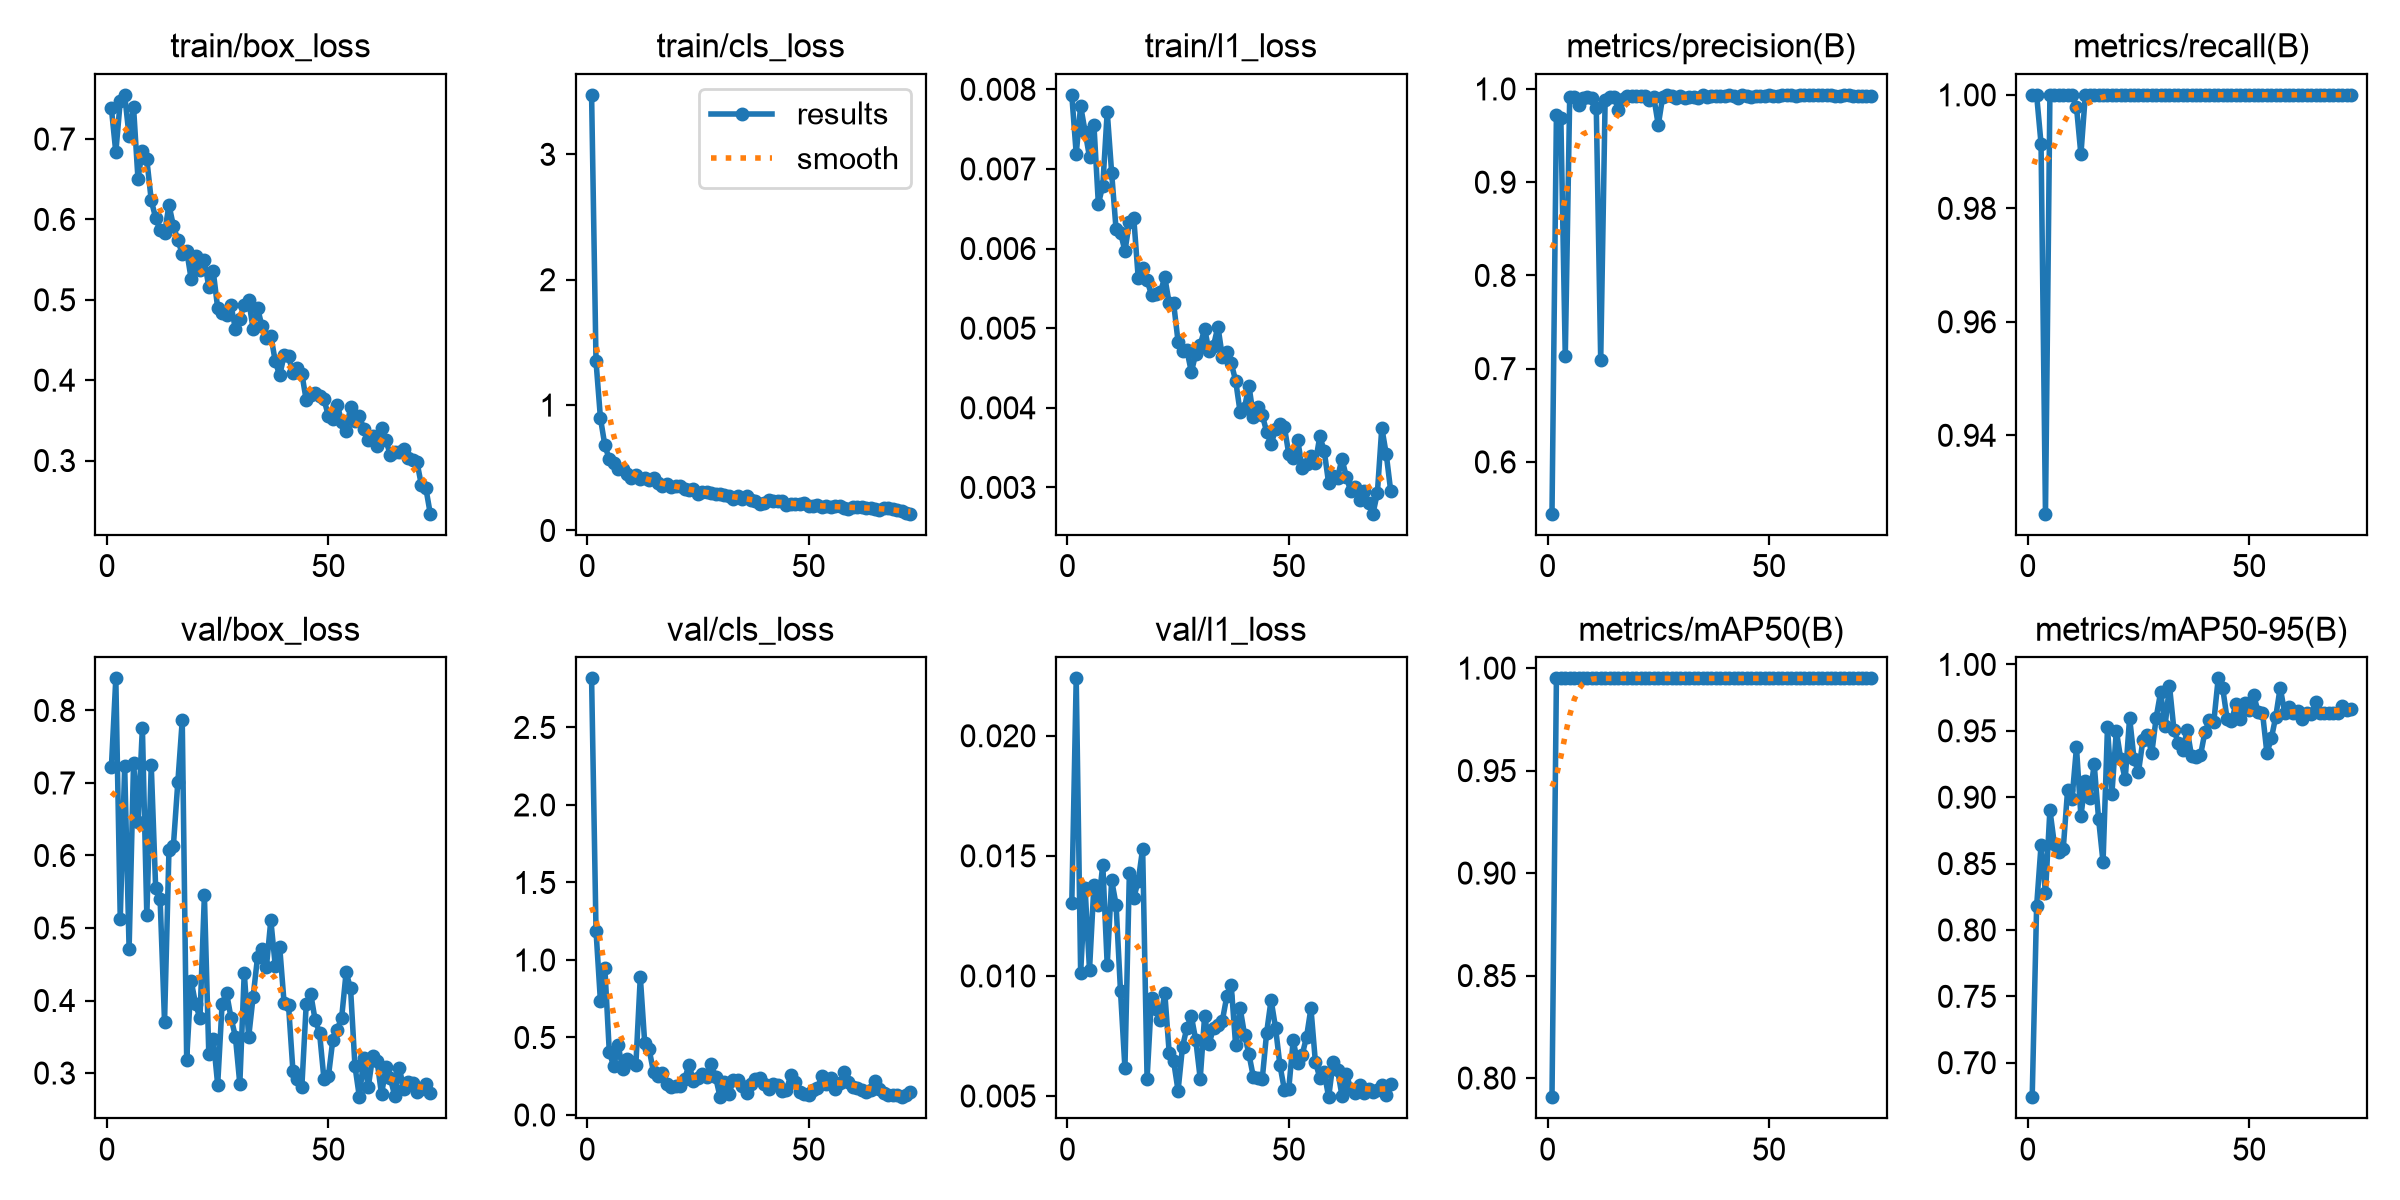
\includegraphics[width=0.9\linewidth]{ia/toy_results.png}
  \caption{Modèle du prototype (YOLO26n, 73 époques)}
\end{subfigure}
\caption{Courbes d'apprentissage : pertes d'entraînement et de validation, précision, rappel et mAP par époque}
\label{fig:courbes}
\end{figure}

\subsection{Sauvegarde et chargement des modèles}
À la fin de chaque notebook, les meilleurs poids sont exportés au format \textbf{ONNX} (\texttt{opset} 17,
graphe simplifié) et copiés dans le dossier \texttt{models/} de l'application, avec les poids PyTorch
(\texttt{.pt}) pour un éventuel réentraînement. Le notebook écrit aussi le profil du modèle et met à jour le
registre \texttt{models/registry.json}, qui contient les métriques d'évaluation affichées dans la page \emph{AI
models}. L'exemple suivant montre le profil du modèle du prototype :

\begin{lstlisting}[language=Python]
{ "name": "Toy track obstacles",
  "models": [ { "id": "toy-obstacles", "path": "models/toy_obstacles.onnx",
                "imgsz": 320, "conf": 0.4,
                "classes": { "column": "column", "box": "box" } } ] }
\end{lstlisting}

Au démarrage, l'application lit le profil de chaque environnement et charge les modèles avec ONNX Runtime ; un
modèle absent est simplement signalé (« pas encore entraîné ») sans empêcher l'application de fonctionner. Le format
ONNX rend l'application indépendante de PyTorch : elle n'a besoin que d'ONNX Runtime, beaucoup plus léger.

% =================================================================================================
\section{Détection et analyse des obstacles}

\subsection{Détection des objets et des anomalies routières}
Pour chaque image, le modèle renvoie une liste de détections : la classe de l'objet, un score de confiance et une
boîte englobante. En environnement réel, les deux modèles routiers analysent la même image et leurs détections
sont réunies.

\subsection{Localisation des objets dans les images}
La boîte indique où se trouve l'objet dans l'image. L'application en déduit deux informations simples :
\begin{itemize}
  \item \textbf{la distance} : plus un objet est proche, plus sa boîte est grande. Connaissant la taille habituelle
        de l'objet (environ 1,7 m pour un piéton, 0,7 m pour un cône), on estime sa distance à partir de la hauteur de
        sa boîte ; pour un nid-de-poule, objet plat, on utilise sa position dans l'image (plus il est bas, plus il est
        proche) ;
  \item \textbf{la position dans la voie} : l'obstacle est « sur la trajectoire » si sa boîte se trouve au centre de
        l'image, devant le véhicule, et « sur le côté » sinon.
\end{itemize}

\subsection{Exploitation des scores de confiance}
Le score de confiance, entre 0 et 1, indique la certitude du modèle. Les détections trop incertaines sont ignorées :
le seuil est de 0,40 pour les usagers de la route et pour le prototype, et de 0,35 pour les anomalies routières afin
de manquer moins de nids-de-poule. La confiance intervient aussi dans la gravité : une détection incertaine compte
moins qu'une détection certaine.

\subsection{Identification des nids-de-poule et des obstacles}
Les \textbf{anomalies fixes} (nid-de-poule, cône, barrière, panneau) sont enregistrées avec leur position sur la carte
et une photo. Les \textbf{usagers de la route} (piéton, cycliste, véhicule, animal) bougent : ils ne sont enregistrés
que s'ils sont devant le véhicule et proches. Un même obstacle vu plusieurs fois n'est enregistré qu'une seule fois,
avec un compteur d'observations. Enfin, un obstacle proche sur la trajectoire fait ralentir ou s'arrêter le véhicule.

\subsection{Estimation de la gravité des anomalies}
Chaque obstacle reçoit un score de gravité de 0 à 100, qui combine quatre éléments :
\begin{equation}
  \text{score} = 100 \times \underbrace{w}_{\text{danger de la classe}} \times
  \underbrace{(0{,}5 + 0{,}5\,p)}_{\text{proximité}} \times \underbrace{c}_{\text{confiance}} \times
  \underbrace{t}_{\text{trajectoire}}
\end{equation}
où $w$ est le poids de danger de la classe (1 pour un piéton, 0,6 pour un nid-de-poule, 0,4 pour un cône…), $p$ la
proximité entre 0 (loin) et 1 (très proche), $c$ la confiance du modèle et $t$ vaut 1 si l'obstacle est sur la
trajectoire et 0,5 s'il est sur le côté. Les poids de danger sont réglables dans l'application.

\subsection{Attribution d'un niveau de priorité}
Le score donne l'un des quatre niveaux de priorité du tableau~\ref{tab:niveaux}. Les obstacles sont ensuite triés du
plus grave au moins grave, pour que l'opérateur traite d'abord les plus dangereux.

\begin{table}[H]
\centering\small
\caption{Niveaux de priorité}
\label{tab:niveaux}
\begin{tabular}{l c l}
\toprule
\textbf{Niveau} & \textbf{Score} & \textbf{Signification} \\
\midrule
\textcolor{critique}{$\blacksquare$} Critique & $\geq 60$ & danger immédiat, à traiter en priorité \\
\textcolor{eleve}{$\blacksquare$} Élevé & 40 -- 60 & danger important \\
\textcolor{moyen}{$\blacksquare$} Moyen & 20 -- 40 & à surveiller \\
\textcolor{faible}{$\blacksquare$} Faible & $< 20$ & information \\
\bottomrule
\end{tabular}
\end{table}

Par exemple, un piéton proche ($p = 0{,}6$), détecté à 90\,\% sur la trajectoire, obtient
$100 \times 1 \times 0{,}8 \times 0{,}9 \times 1 = 72$ : il est \textbf{critique}. Un cône sur le côté, dans les mêmes
conditions, obtient $100 \times 0{,}4 \times 0{,}8 \times 0{,}9 \times 0{,}5 = 14{,}4$ : il est \textbf{faible}.

% =================================================================================================
\section{Évaluation des performances}

\subsection{Méthodologie d'évaluation}
Toutes les métriques finales sont mesurées sur les \textbf{ensembles de test}, jamais utilisés pendant l'entraînement
ni pour choisir les réglages. Pour le modèle routier, le réglage d'inférence (taille d'entrée, augmentation au
moment du test) a été choisi sur l'ensemble de validation, puis appliqué une seule fois au test. Nous indiquons
toujours le réglage correspondant à chaque résultat. Ultralytics donne la précision et le rappel au seuil de
confiance qui maximise le score F1 moyen ; les matrices de confusion sont calculées au seuil réellement utilisé dans
l'application.

\subsection{Précision, rappel et score F1}
Une détection est un \textbf{vrai positif} (TP) si elle correspond à un objet réel de la même classe, un
\textbf{faux positif} (FP) sinon ; un objet réel non détecté est un \textbf{faux négatif} (FN). On définit :
\begin{equation}
  \text{Précision} = \frac{TP}{TP + FP}, \qquad
  \text{Rappel} = \frac{TP}{TP + FN}, \qquad
  F_1 = 2 \cdot \frac{\text{Précision} \times \text{Rappel}}{\text{Précision} + \text{Rappel}}
\end{equation}
La précision mesure la fiabilité des alertes (peu de fausses alarmes), le rappel la capacité à ne pas manquer
d'obstacles. Pour un véhicule, un rappel élevé est souvent prioritaire, mais trop de fausses alarmes rendraient le
système inutilisable : le score F1 résume ce compromis.

\subsection{Intersection sur l'union (IoU) et mAP}
Pour décider si une boîte prédite correspond à un objet réel, on mesure leur recouvrement par l'\textbf{intersection
sur l'union} (figure~\ref{fig:iou}) :
\begin{equation} \text{IoU}(A, B) = \frac{|A \cap B|}{|A \cup B|} \end{equation}
Une prédiction est correcte si son IoU avec un objet réel dépasse un seuil (0,5 en général).

\begin{figure}[H]
\centering
\begin{tikzpicture}
  \fill[bleufst!25] (0,0) rectangle (2.4,1.8); \fill[orangefst!35] (1.2,0.6) rectangle (3.4,2.4);
  \fill[vertfst!70] (1.2,0.6) rectangle (2.4,1.8);
  \draw[thick,bleufst] (0,0) rectangle (2.4,1.8); \draw[thick,orangefst] (1.2,0.6) rectangle (3.4,2.4);
  \node[font=\scriptsize] at (0.55,0.3) {réelle}; \node[font=\scriptsize] at (2.95,2.15) {prédite};
  \node at (4.4,1.2) {$\text{IoU} = $};
  \begin{scope}[shift={(4.85,1.35)},scale=0.5]
    \fill[vertfst!70] (1.2,0.6) rectangle (2.4,1.8); \draw[thick,vertfst!60!black] (1.2,0.6) rectangle (2.4,1.8);
    \node[font=\scriptsize,anchor=west] at (3.6,1.2) {intersection};
  \end{scope}
  \draw[thick] (4.9,1.2) -- (6.7,1.2);
  \begin{scope}[shift={(4.95,-0.15)},scale=0.5]
    \fill[vertfst!40] (0,0) rectangle (2.4,1.8) (1.2,0.6) rectangle (3.4,2.4);
    \draw[thick,vertfst!60!black] (0,0) -- (2.4,0) -- (2.4,0.6) -- (3.4,0.6) -- (3.4,2.4) -- (1.2,2.4) -- (1.2,1.8)
                                  -- (0,1.8) -- cycle;
    \node[font=\scriptsize,anchor=west] at (3.6,1.2) {union};
  \end{scope}
\end{tikzpicture}
\caption{Intersection sur l'union entre une boîte réelle et une boîte prédite}
\label{fig:iou}
\end{figure}

En faisant varier le seuil de confiance, on obtient une courbe précision-rappel ; l'aire sous cette courbe est la
\textbf{précision moyenne} (AP) d'une classe. Le \textbf{mAP} est la moyenne des AP sur toutes les
classes~\cite{everingham2010voc,padilla2020metrics} :
\begin{itemize}
  \item \textbf{mAP@50} : IoU minimale de 0,5 ;
  \item \textbf{mAP@50-95} : moyenne des mAP pour des seuils d'IoU de 0,50 à 0,95 par pas de 0,05, plus exigeante
        sur la précision de localisation.
\end{itemize}

\subsection{Temps d'inférence et vitesse de traitement}
La vitesse est mesurée à deux niveaux (tableau~\ref{tab:vitesse}). Sur le GPU d'entraînement, Ultralytics mesure le
temps d'inférence pur par image. Dans l'application, les modèles ONNX s'exécutent sur le processeur de
l'ordinateur ; le temps dépend alors de la charge de la machine, car l'application, les simulateurs et le flux
vidéo partagent le même processeur.

\begin{table}[H]
\centering\small
\caption{Temps d'inférence mesurés}
\label{tab:vitesse}
\begin{tabularx}{\linewidth}{X l l}
\toprule
\textbf{Modèle et conditions} & \textbf{Temps par image} & \textbf{Cadence} \\
\midrule
Anomalies routières, GPU, 640 px & 10 ms & — \\
Anomalies routières, GPU, 960 px + TTA & 50 ms & — \\
Prototype, GPU, 320 px & 22 ms (30 ms en test ESP32) & — \\
Application, CPU : usagers + anomalies en parallèle (machine peu chargée) & $\approx$ 190 ms & $\approx$ 5 images/s \\
Application, CPU : usagers + anomalies (machine chargée) & $\approx$ 730 ms & $\approx$ 1,4 image/s \\
Application, CPU : modèle du prototype (image 480\,$\times$\,640) & $\approx$ 70 ms & $\approx$ 14 images/s \\
\bottomrule
\end{tabularx}
\end{table}

\subsection{Résultats obtenus sur les données réelles}\label{sec:resultats-reels}
Le tableau~\ref{tab:res-reel} donne les résultats du détecteur d'anomalies routières sur les 815 images de test
(5\,105 objets), au réglage temps réel utilisé dans l'application (640 px) et au meilleur réglage hors ligne
(960 px avec augmentation au moment du test, TTA).

\begin{table}[H]
\centering\small
\caption{Résultats du détecteur d'anomalies routières sur l'ensemble de test}
\label{tab:res-reel}
\begin{tabular}{l r cccc c cccc}
\toprule
 & & \multicolumn{4}{c}{\textbf{640 px (temps réel)}} & & \multicolumn{4}{c}{\textbf{960 px + TTA}} \\
\cmidrule{3-6}\cmidrule{8-11}
\textbf{Classe} & \textbf{Objets} & P & R & mAP50 & mAP50-95 & & P & R & mAP50 & mAP50-95 \\
\midrule
nid-de-poule & 299  & 0,601 & 0,254 & 0,312 & 0,108 & & 0,626 & 0,268 & 0,330 & 0,119 \\
cône         & 2\,358 & 0,712 & 0,715 & 0,694 & 0,416 & & 0,681 & 0,763 & 0,744 & 0,464 \\
barrière     & 1\,977 & 0,692 & 0,539 & 0,578 & 0,317 & & 0,688 & 0,594 & 0,634 & 0,369 \\
panneau      & 471  & 0,638 & 0,495 & 0,520 & 0,367 & & 0,630 & 0,567 & 0,588 & 0,430 \\
\midrule
\textbf{toutes} & \textbf{5\,105} & \textbf{0,661} & \textbf{0,501} & \textbf{0,526} & \textbf{0,302} & &
  \textbf{0,656} & \textbf{0,548} & \textbf{0,574} & \textbf{0,346} \\
\bottomrule
\end{tabular}
\end{table}

Les cônes et les barrières, nombreux et bien contrastés, sont les mieux reconnus. Les nids-de-poule restent
difficiles (AP@50 de 0,31) : ils sont peu nombreux dans l'ensemble (299 objets de test) et visuellement très
variables. Le réglage 960 px + TTA améliore le mAP@50 de 0,526 à 0,574, au prix d'un temps d'inférence cinq fois
plus long ; il n'est donc pas utilisé en temps réel.

Deux analyses complémentaires éclairent ces chiffres. D'une part, si l'on ne demande au modèle que de \emph{trouver}
l'obstacle sans en nommer le type exact (évaluation agnostique de la classe, un cône pris pour une barrière restant
une détection correcte), le mAP@50 atteint 0,630 en temps réel et 0,677 au meilleur réglage
(tableau~\ref{tab:agnostique}). D'autre part, le seuil de confiance règle le compromis entre fausses alarmes et
obstacles manqués : à un seuil de 0,70, la précision moyenne atteint 0,916, mais le rappel tombe à 0,300.

\begin{table}[H]
\centering\small
\caption{Évaluation agnostique de la classe et points de fonctionnement (ensemble de test)}
\label{tab:agnostique}
\begin{tabular}{lccccc}
\toprule
\textbf{Évaluation agnostique} & P & R & F1 & mAP50 & mAP50-95 \\
\midrule
640 px (temps réel) & 0,726 & 0,597 & 0,655 & 0,630 & 0,364 \\
960 px + TTA & 0,711 & 0,646 & 0,677 & 0,677 & 0,412 \\
\bottomrule
\end{tabular}

\vspace{0.3cm}
\begin{tabular}{ccccc}
\toprule
\textbf{Seuil de confiance} & \textbf{P (par classe)} & \textbf{R (par classe)} & \textbf{P (agnostique)} &
\textbf{R (agnostique)} \\
\midrule
0,25 & 0,520 & 0,612 & 0,563 & 0,720 \\
0,40 & 0,673 & 0,534 & 0,707 & 0,647 \\
0,50 & 0,763 & 0,474 & 0,781 & 0,579 \\
0,70 & 0,916 & 0,300 & 0,893 & 0,370 \\
\bottomrule
\end{tabular}
\end{table}

La figure~\ref{fig:courbes-reel} présente les courbes précision-rappel et F1 ainsi que la matrice de confusion au
seuil utilisé dans l'application (0,35). La matrice montre que les confusions entre classes sont rares (au plus
3\,\%) : les erreurs sont surtout des objets manqués (ligne \emph{background}) et des fausses détections sur le
fond, en particulier des cônes.

\begin{figure}[H]
\centering
\begin{subfigure}[b]{0.49\linewidth}\centering
  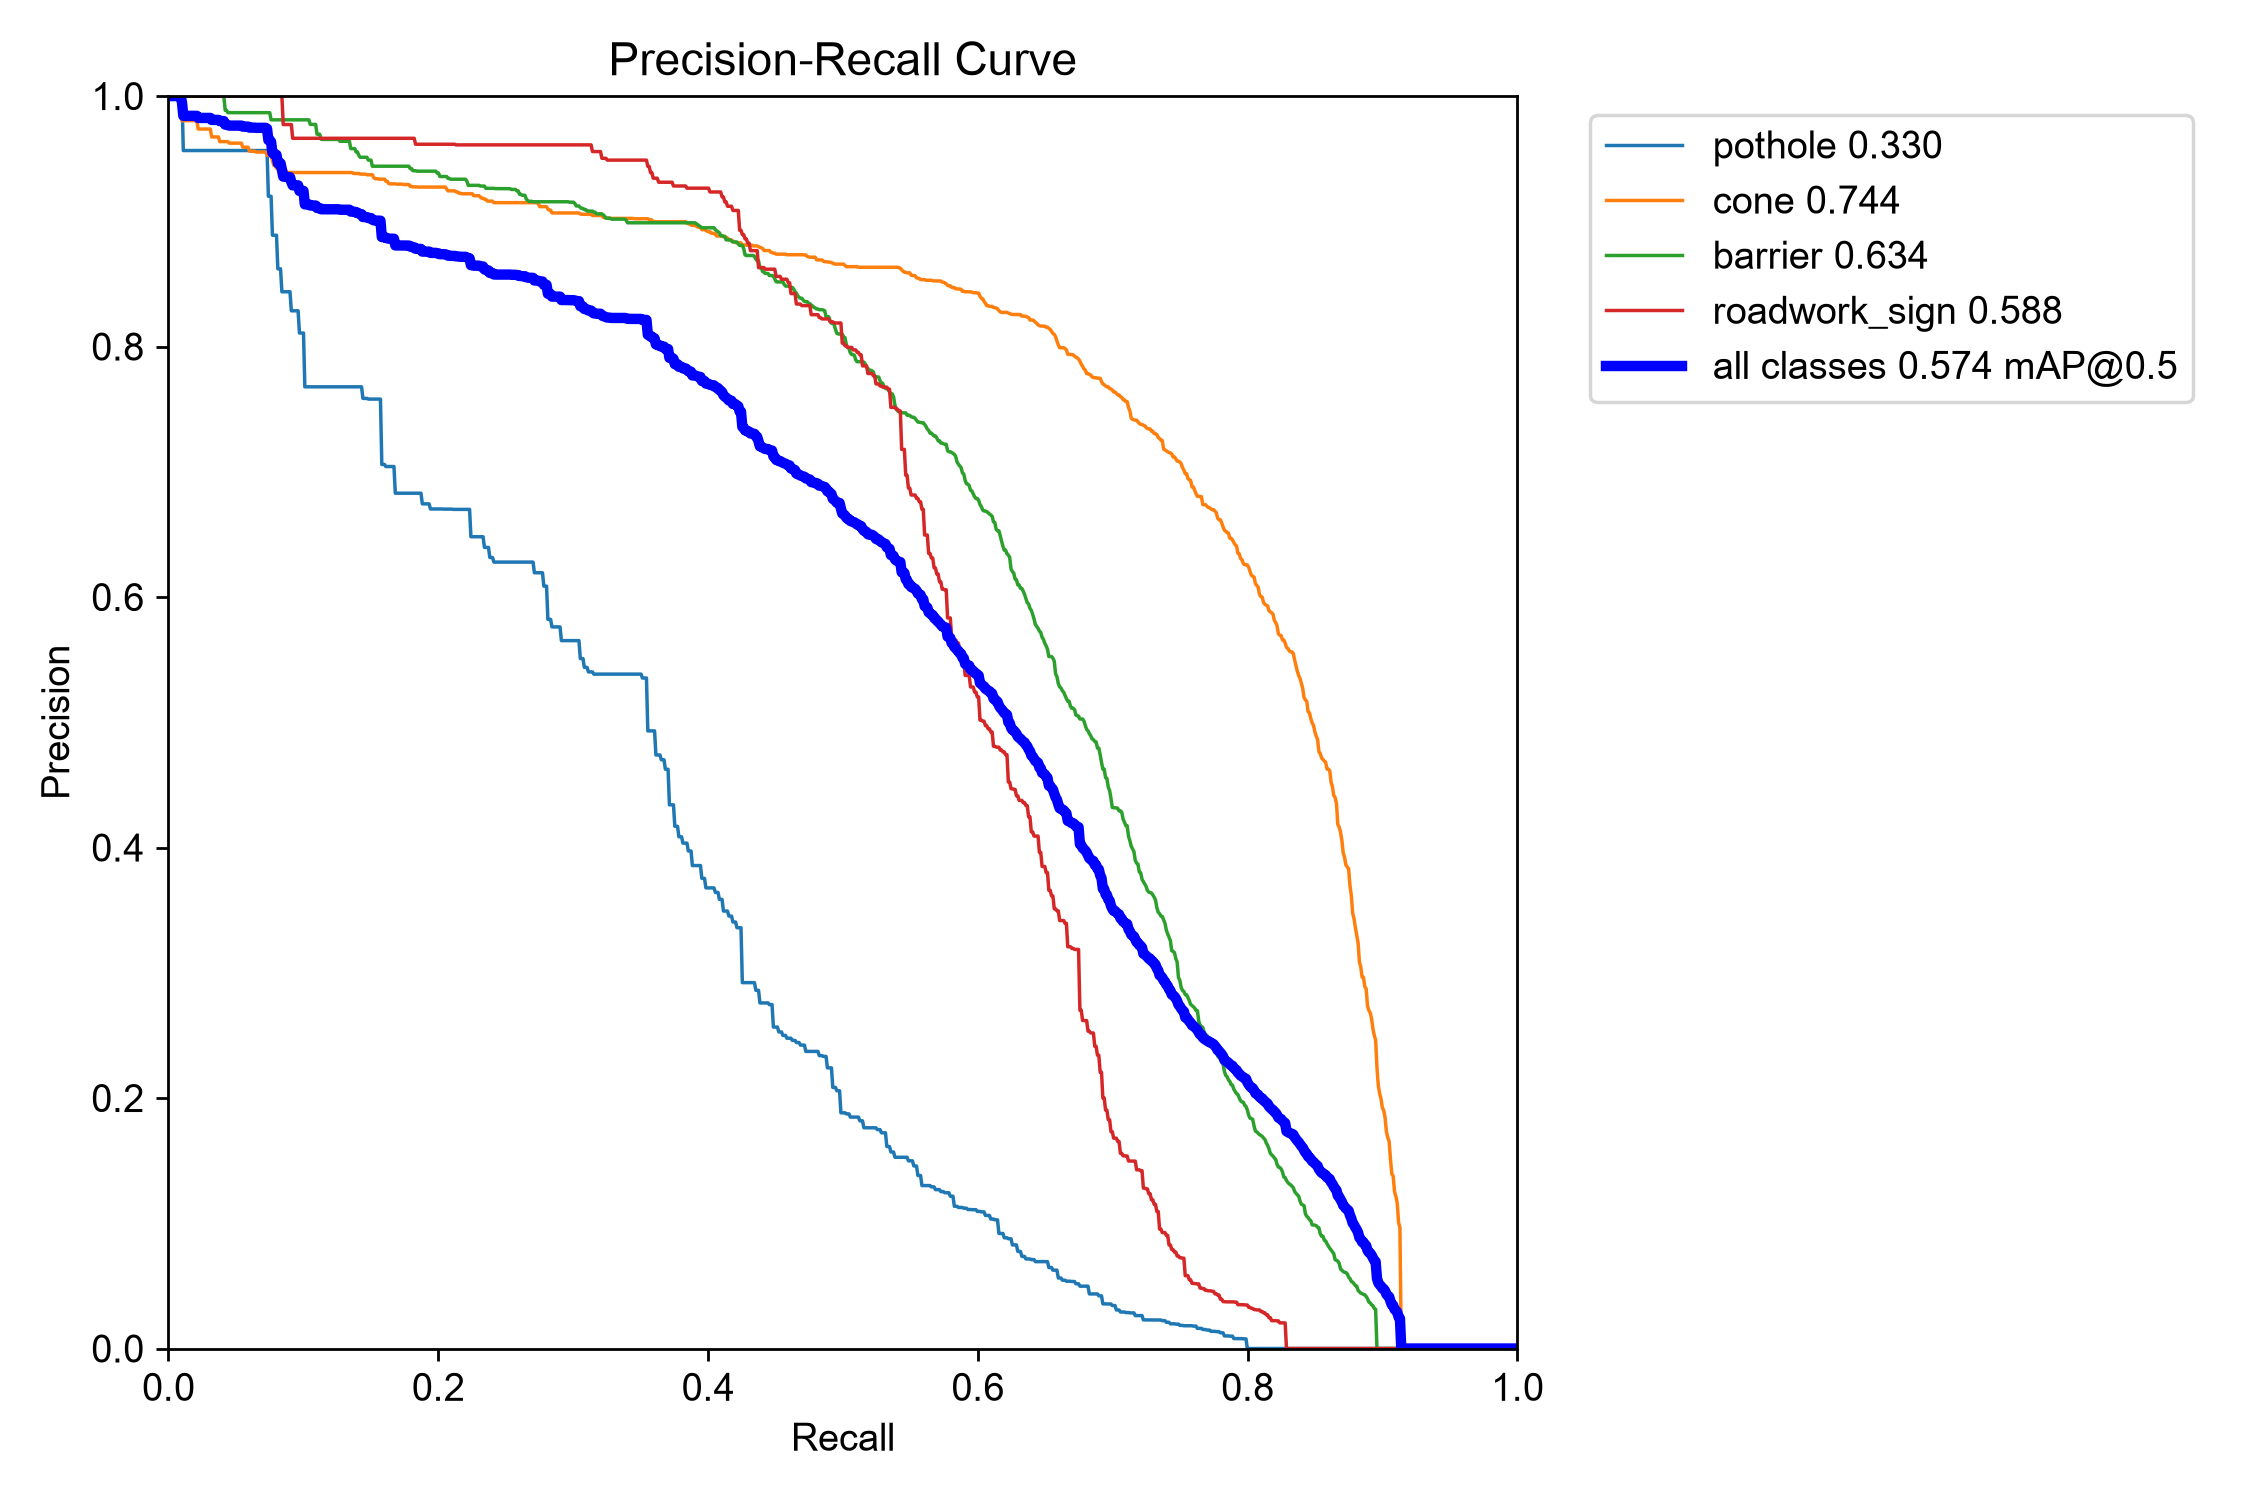
\includegraphics[width=\linewidth]{ia/reel_pr.png}
  \caption{Courbes précision-rappel (960 px + TTA)}
\end{subfigure}\hfill
\begin{subfigure}[b]{0.49\linewidth}\centering
  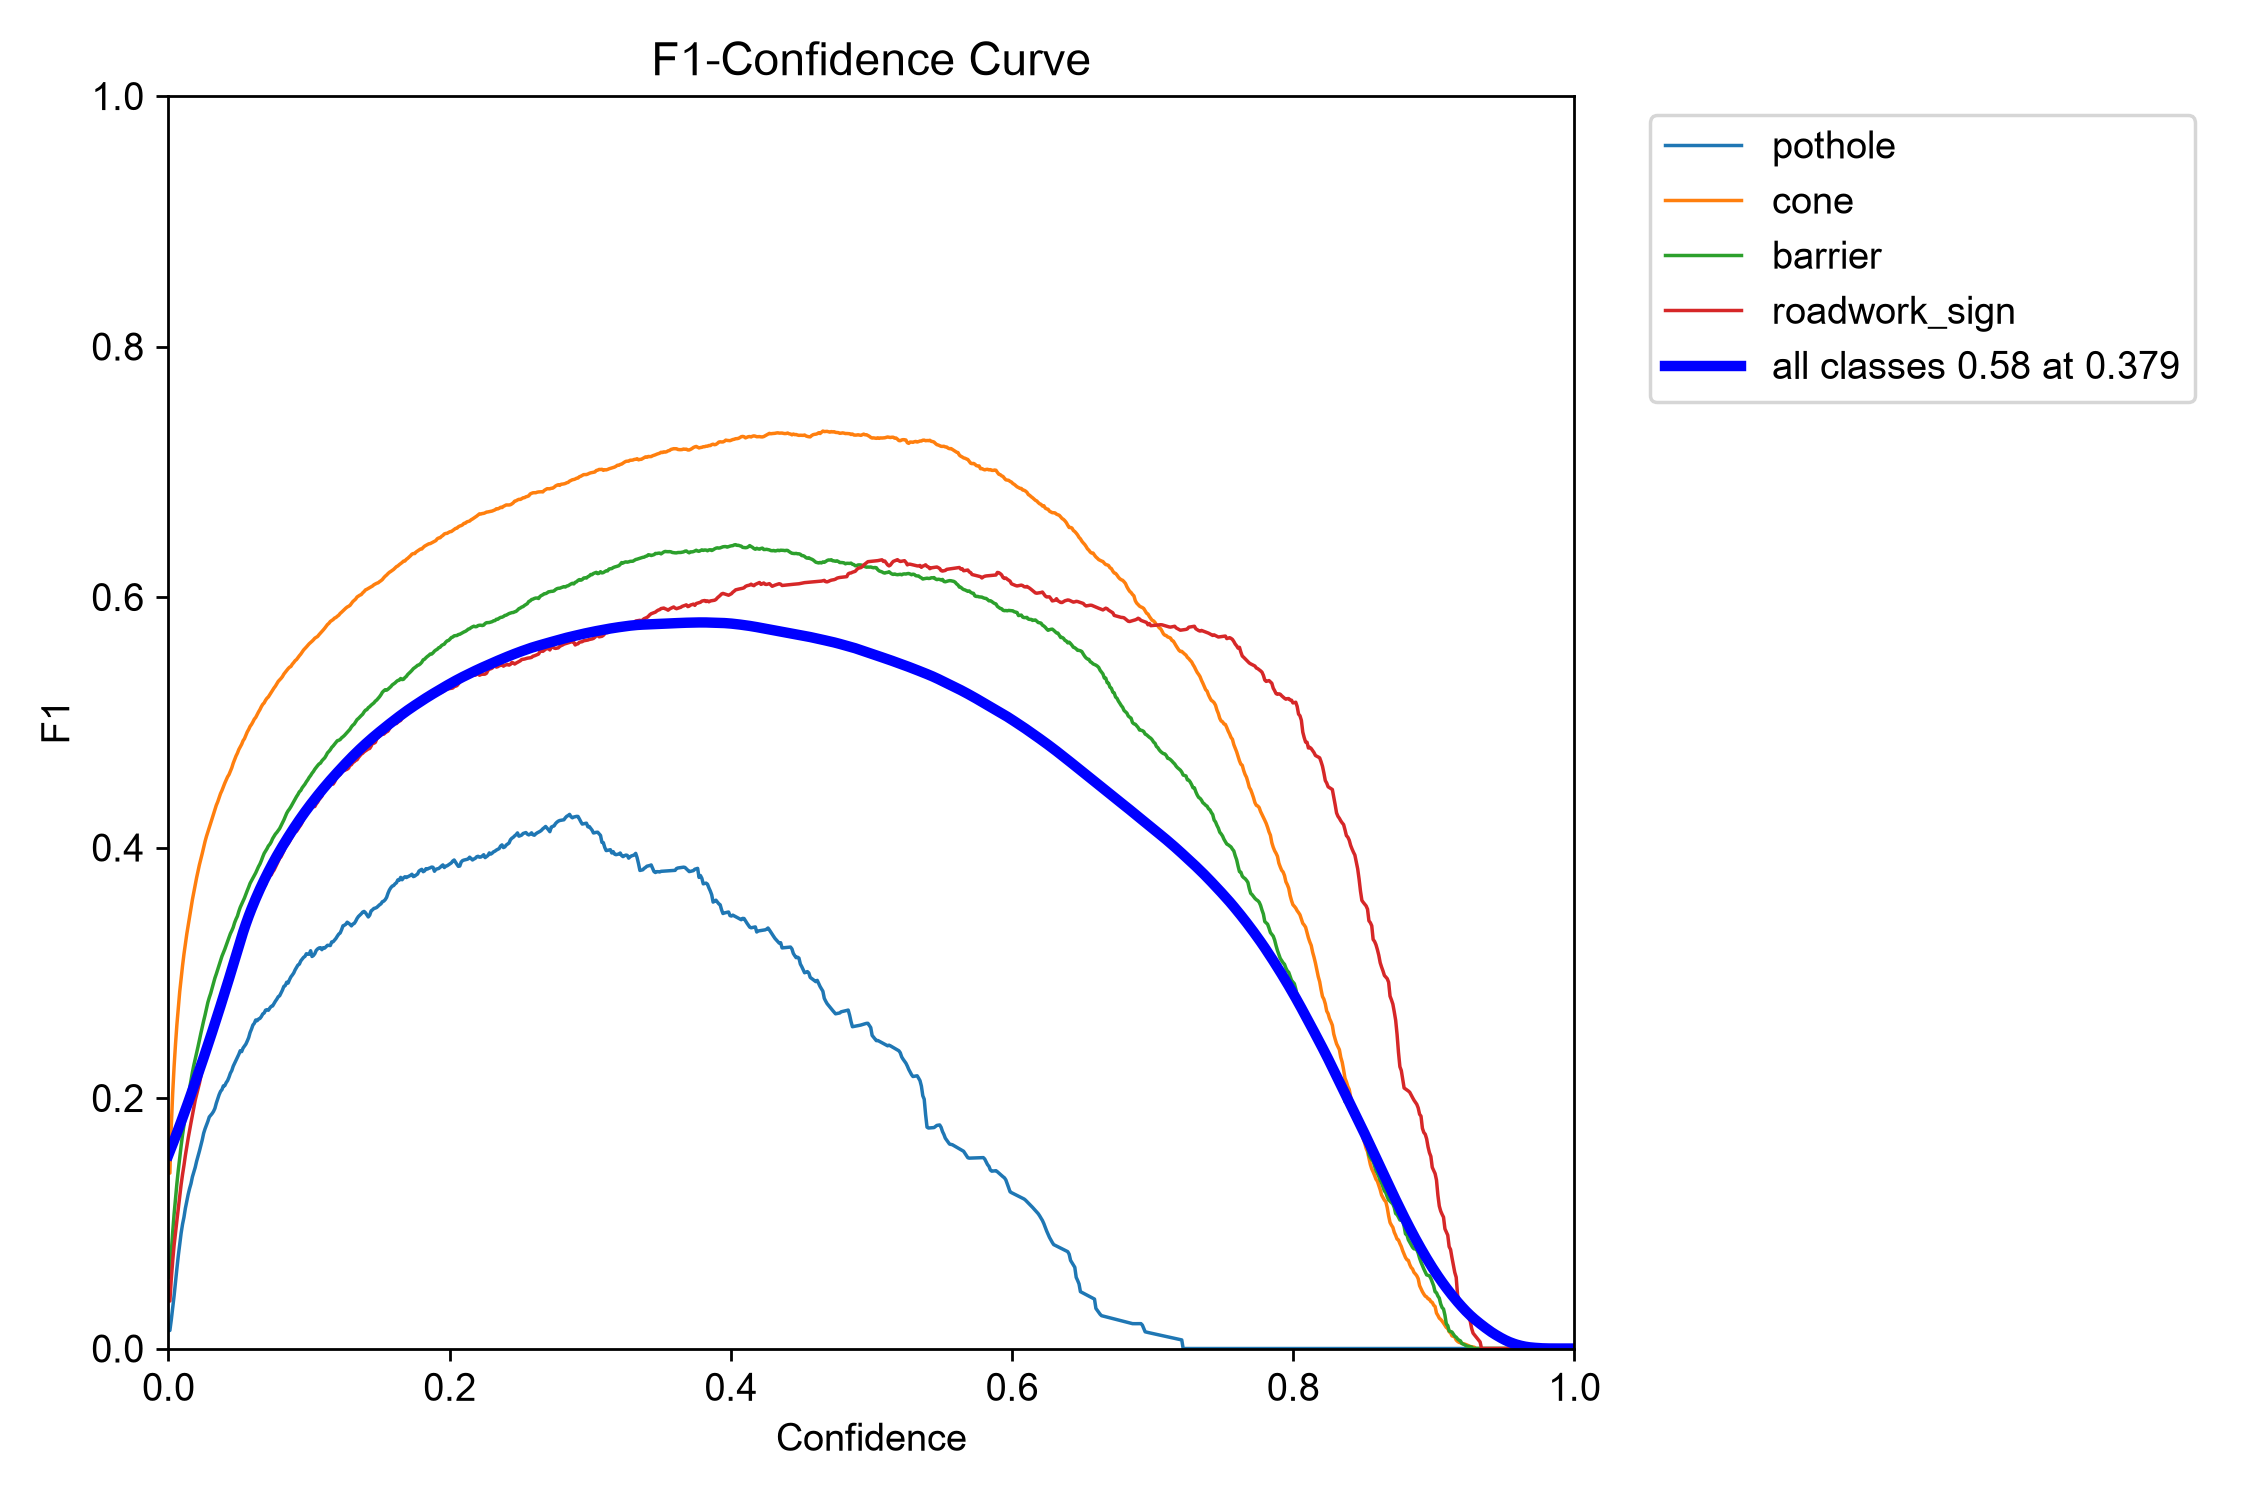
\includegraphics[width=\linewidth]{ia/reel_f1.png}
  \caption{Score F1 en fonction du seuil}
\end{subfigure}

\vspace{0.2cm}
\begin{subfigure}[b]{0.62\linewidth}\centering
  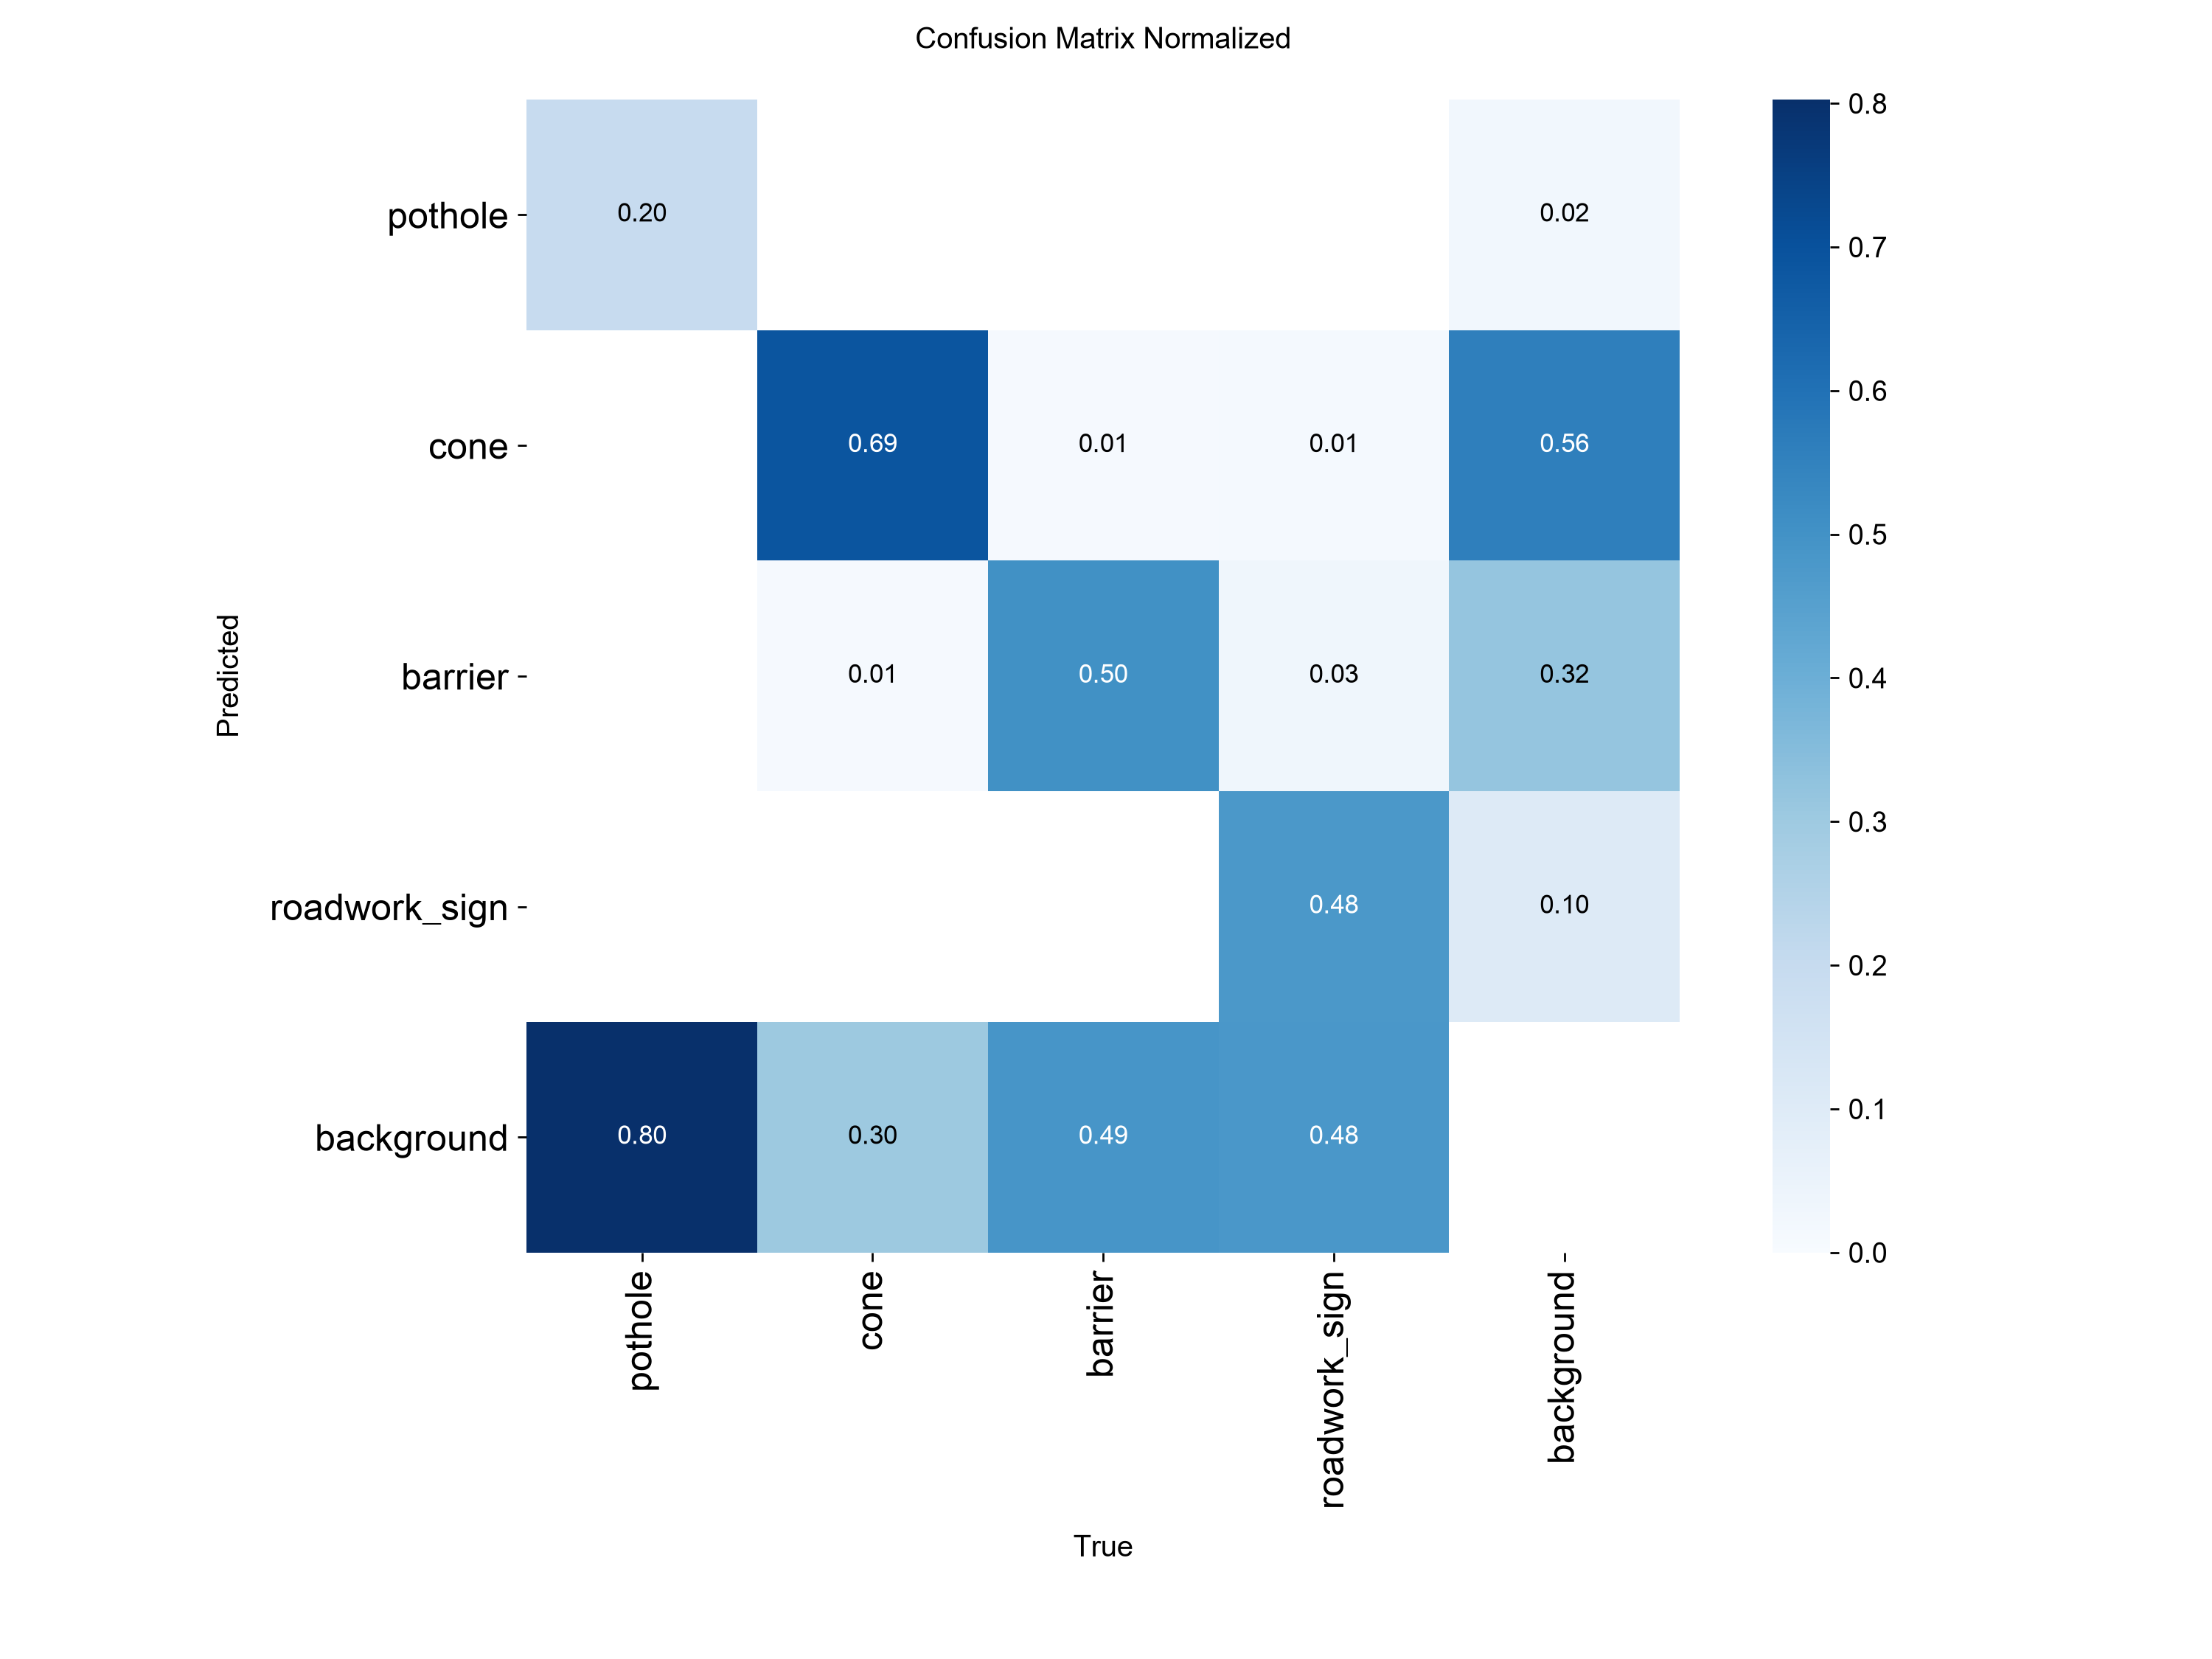
\includegraphics[width=\linewidth]{ia/reel_confusion.png}
  \caption{Matrice de confusion normalisée (640 px, seuil 0,35)}
\end{subfigure}
\caption{Résultats du détecteur d'anomalies routières sur l'ensemble de test}
\label{fig:courbes-reel}
\end{figure}

\subsection{Résultats obtenus sur les données du prototype}
Le tableau~\ref{tab:res-proto} donne les résultats du modèle du prototype sur ses deux ensembles de test. Au seuil
de 0,40 utilisé dans l'application, les 15 obstacles des images de test sont tous détectés avec la bonne classe,
sans aucune fausse détection, aussi bien sur les images d'origine que sur leurs versions au style ESP32-CAM
(tableau~\ref{tab:conf-proto}). Le mAP@50-95 plus faible sur les images ESP32-CAM (0,921 contre 0,976) traduit des
boîtes un peu moins précises sur des images petites et dégradées.

\begin{table}[H]
\centering\small
\caption{Résultats du modèle du prototype sur l'ensemble de test (26 images, 15 obstacles)}
\label{tab:res-proto}
\begin{tabular}{lccccc}
\toprule
\textbf{Ensemble de test} & P & R & F1 & mAP50 & mAP50-95 \\
\midrule
Images d'origine (832\,$\times$\,464) & 0,989 & 1,000 & 0,994 & 0,995 & 0,976 \\
Mêmes images au style ESP32-CAM (320\,$\times$\,240) & 0,991 & 1,000 & 0,995 & 0,995 & 0,921 \\
\bottomrule
\end{tabular}
\end{table}

\begin{table}[H]
\centering\small
\caption{Matrice de confusion du modèle du prototype (test, seuil 0,40)}
\label{tab:conf-proto}
\begin{tabular}{l|ccc}
\toprule
\textbf{Réel $\backslash$ prédit} & \textbf{colonne} & \textbf{boîte} & \textbf{fond (manqué)} \\
\midrule
colonne & 6 & 0 & 0 \\
boîte & 0 & 9 & 0 \\
fond (fausse détection) & 0 & 0 & — \\
\bottomrule
\end{tabular}
\end{table}

\begin{figure}[H]
\centering
\begin{subfigure}[b]{0.49\linewidth}\centering
  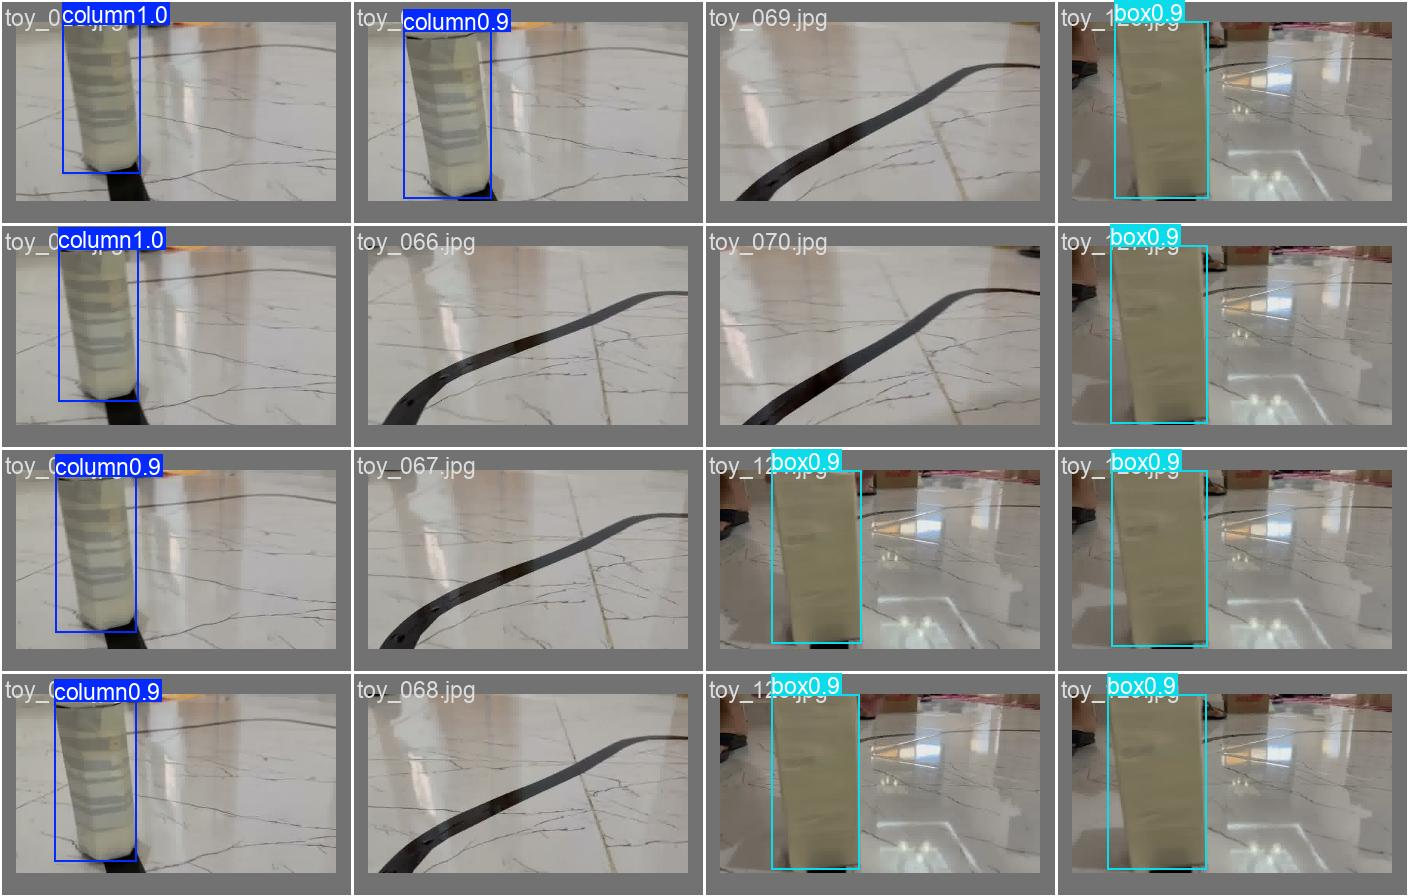
\includegraphics[width=\linewidth]{ia/toy_test_pred.jpg}
  \caption{Images de test d'origine}
\end{subfigure}\hfill
\begin{subfigure}[b]{0.49\linewidth}\centering
  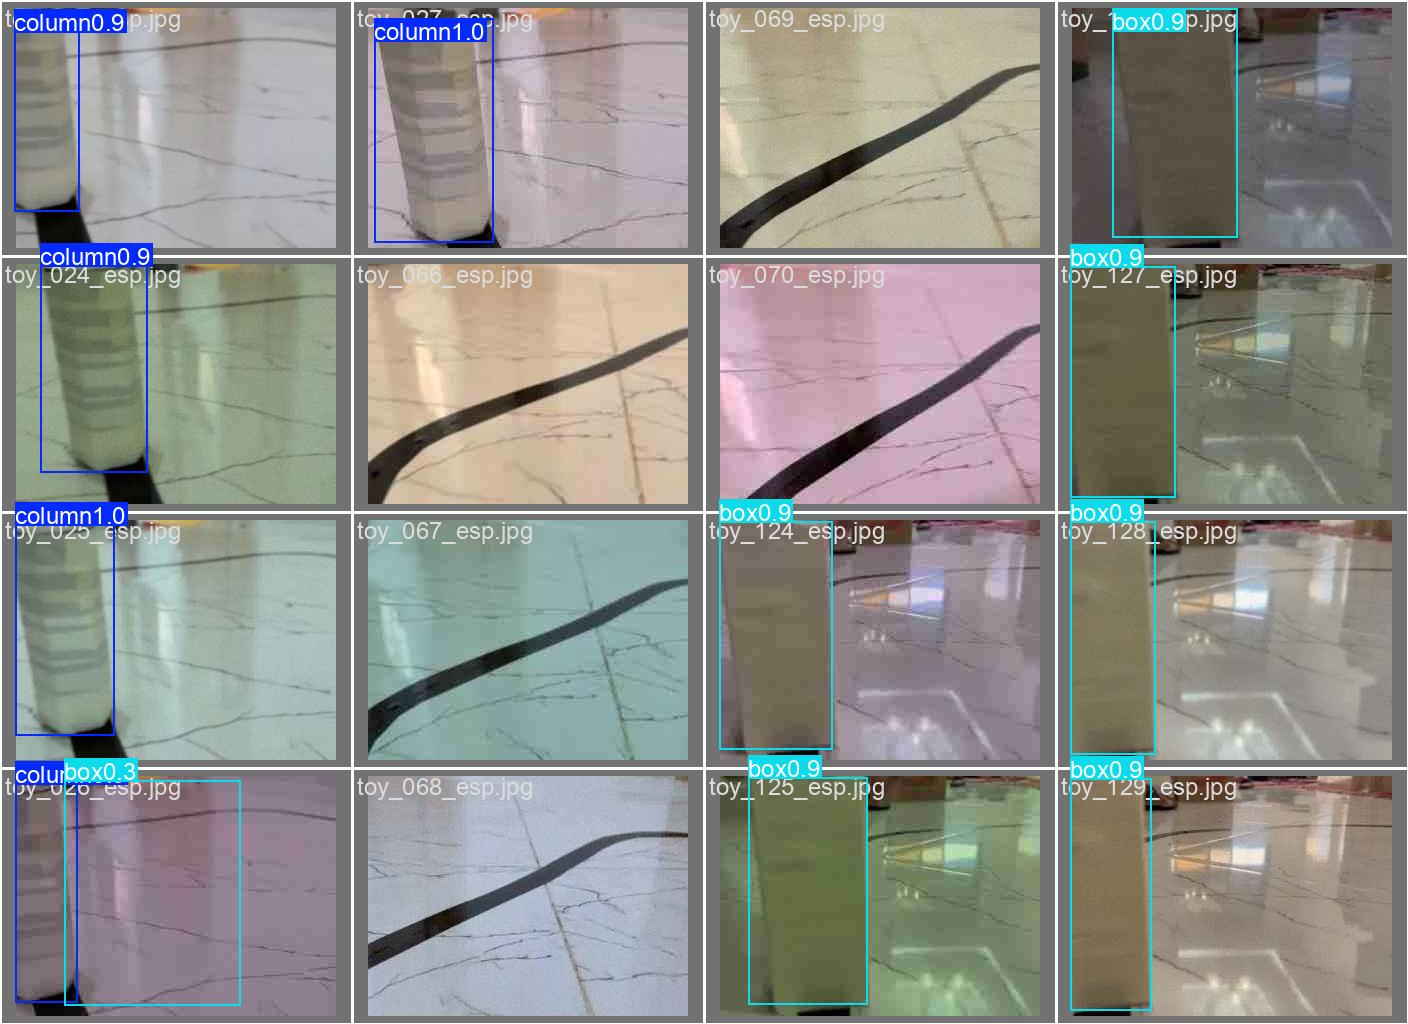
\includegraphics[width=\linewidth]{ia/toy_test_esp32_pred.jpg}
  \caption{Images de test au style ESP32-CAM}
\end{subfigure}

\vspace{0.2cm}
\begin{subfigure}[b]{0.49\linewidth}\centering
  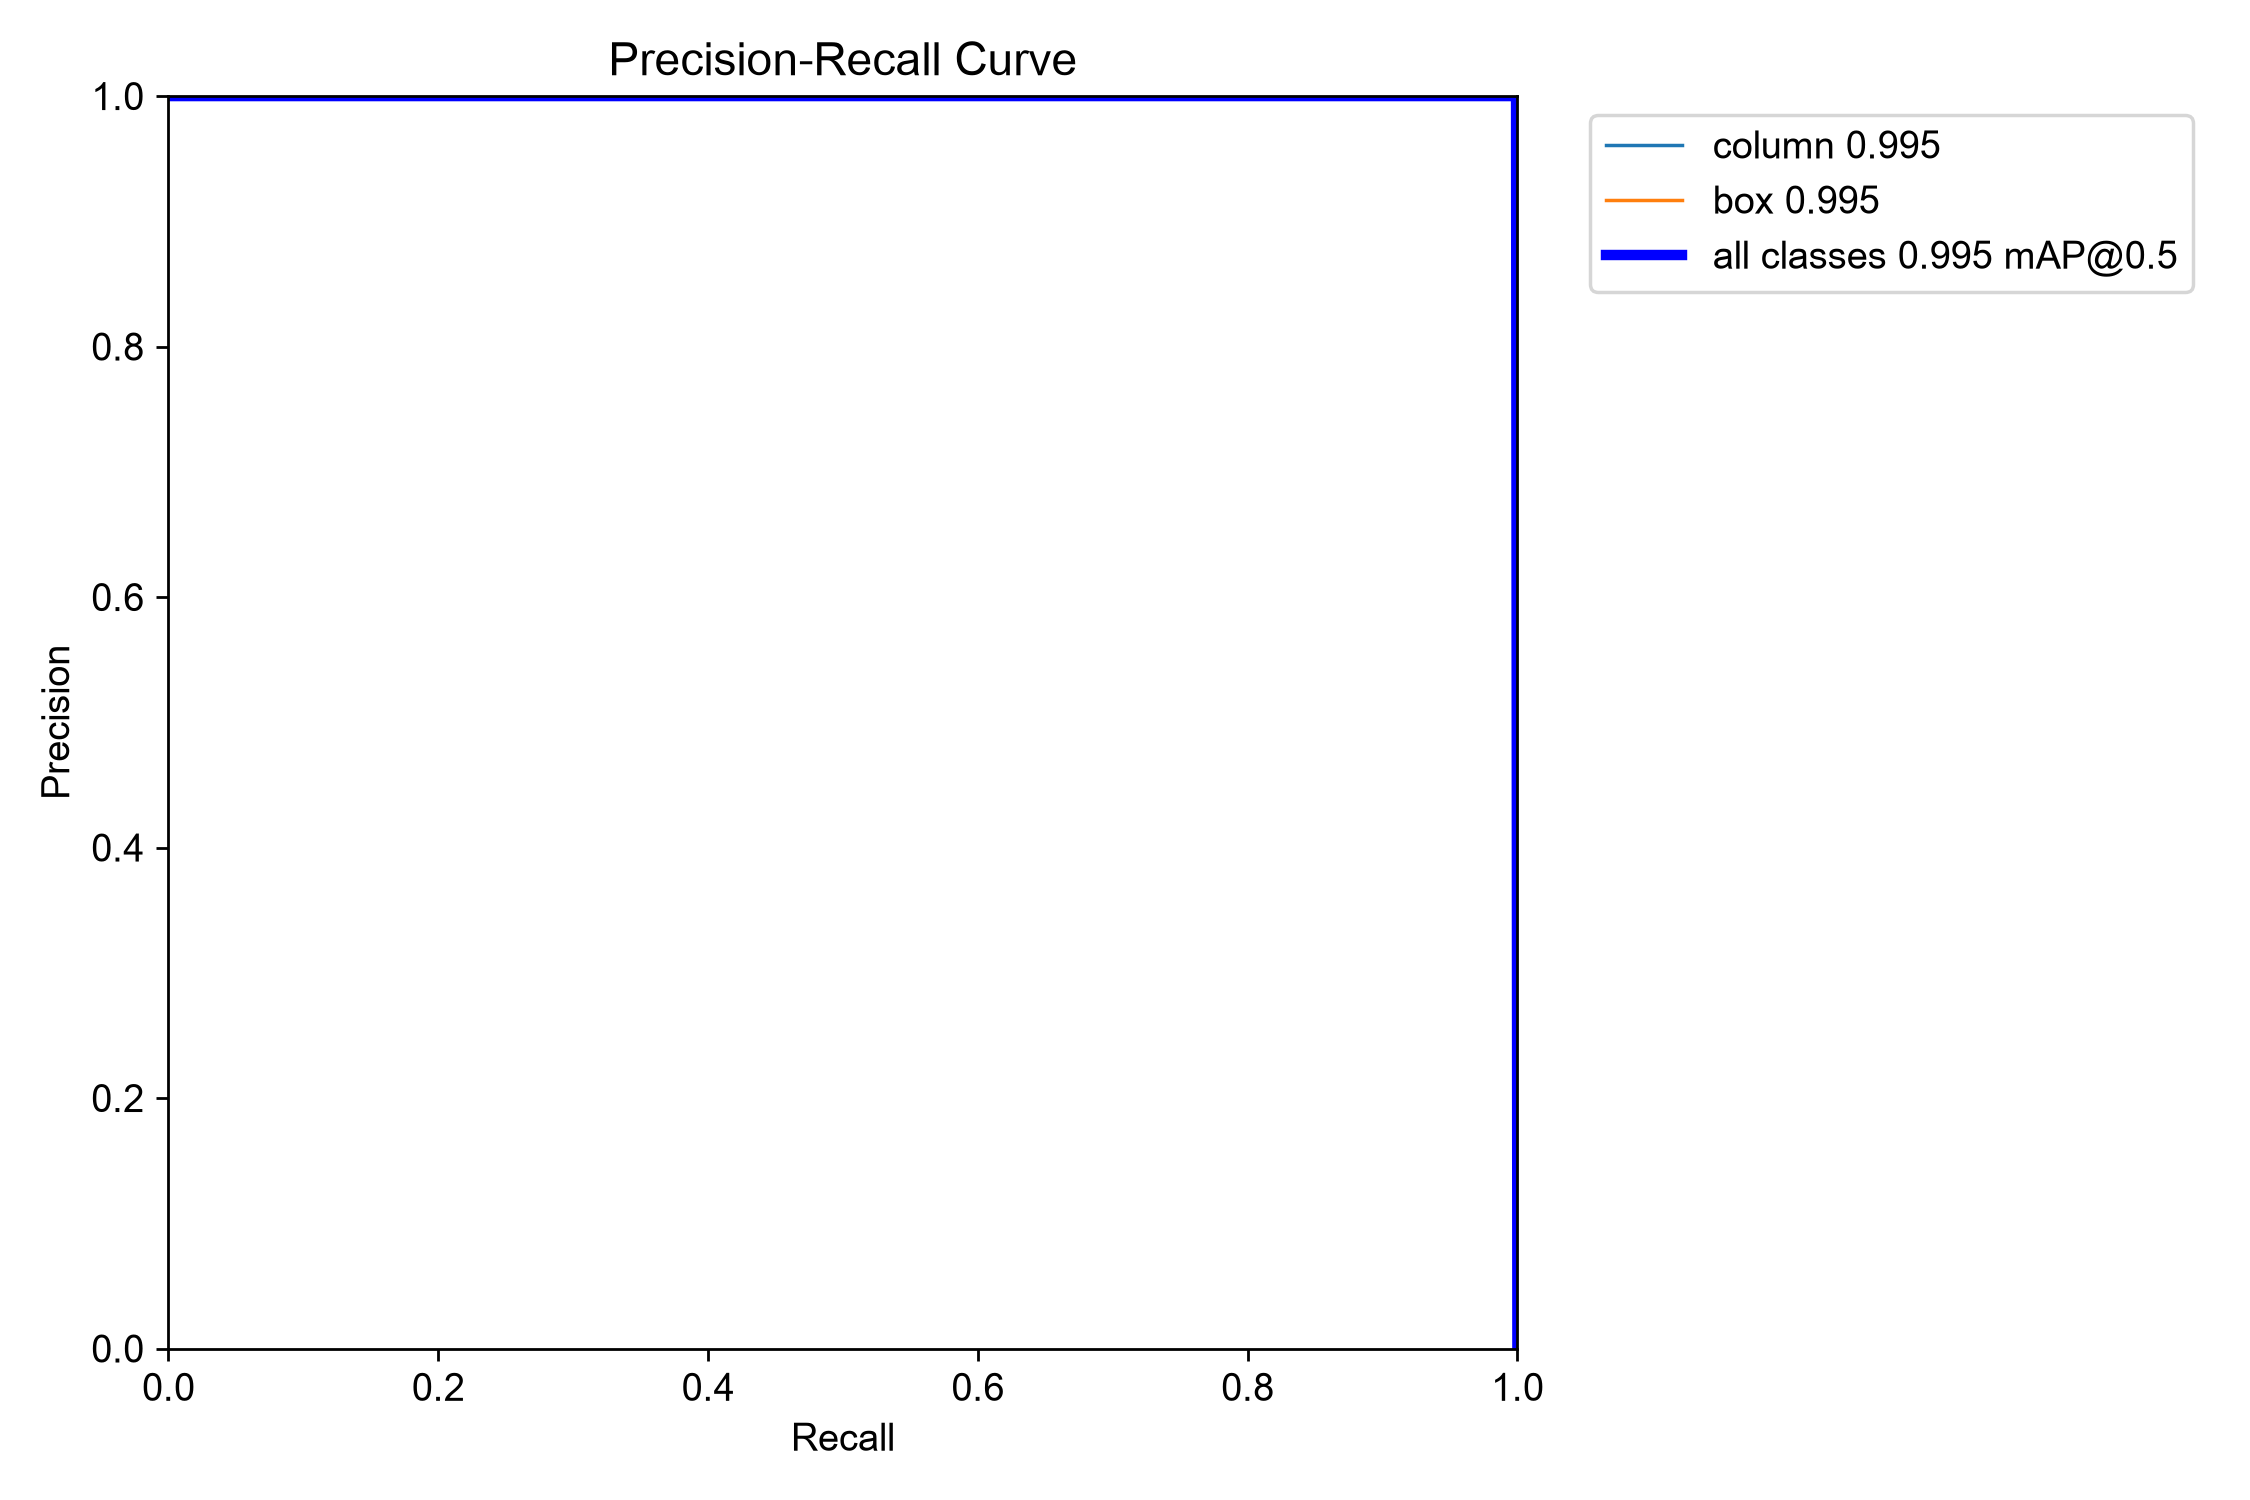
\includegraphics[width=\linewidth]{ia/toy_pr.png}
  \caption{Courbe précision-rappel}
\end{subfigure}\hfill
\begin{subfigure}[b]{0.49\linewidth}\centering
  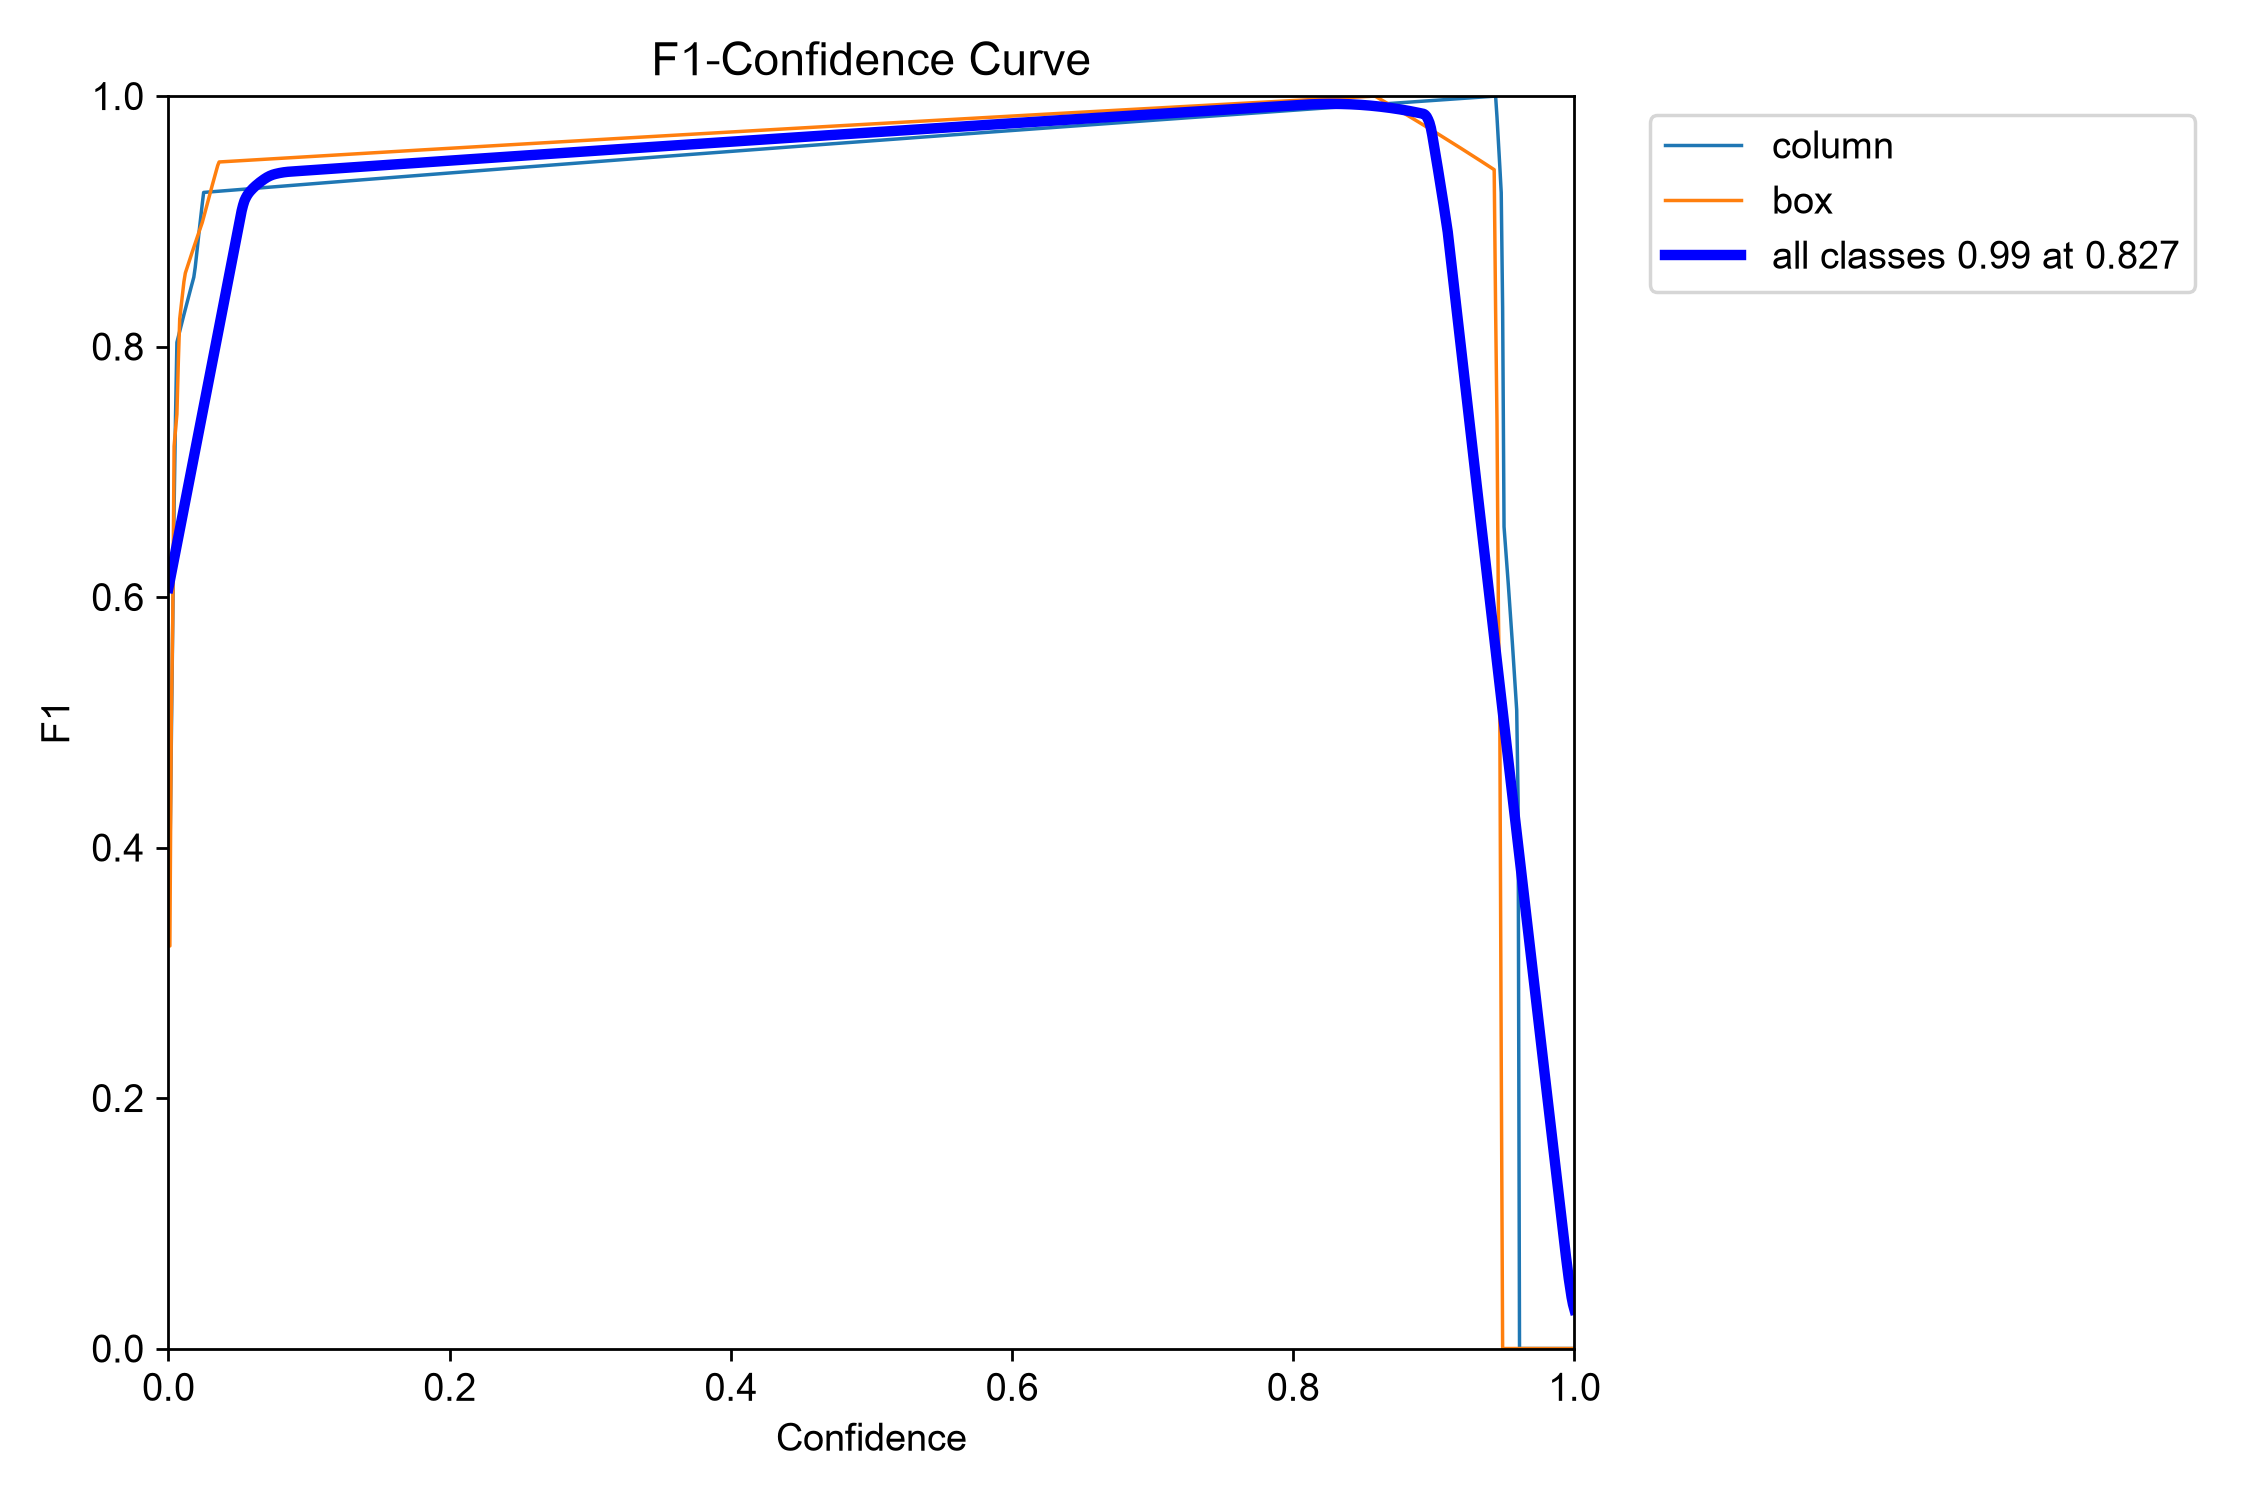
\includegraphics[width=\linewidth]{ia/toy_f1.png}
  \caption{Score F1 en fonction du seuil}
\end{subfigure}
\caption{Résultats du modèle du prototype sur l'ensemble de test}
\label{fig:res-proto}
\end{figure}

Ces résultats doivent être nuancés. L'ensemble de test est petit et provient de la même vidéo que l'entraînement
(même éclairage, même sol), même si le découpage temporel évite les quasi-doublons. Le test sur la vraie caméra
de la voiture, réalisé après l'entraînement, confirme que la boîte est reconnue avec une confiance de 95\,\%
(figure~\ref{fig:test-reel-proto}) ; il a aussi révélé deux limites. D'une part, la caméra étant montée sur la
tranche, l'image doit être redressée avant l'analyse : sans rotation, le modèle ne détecte rien. D'autre part, des
éléments jamais vus pendant l'entraînement, comme un meuble brun en bord d'image ou une main devant l'objectif,
ont parfois été pris pour une colonne. L'enregistrement d'images réelles de l'ESP32-CAM, prévu dans l'application,
permettra d'ajouter ces cas à l'entraînement.

\begin{figure}[H]
\centering
\begin{subfigure}[b]{0.52\linewidth}\centering
  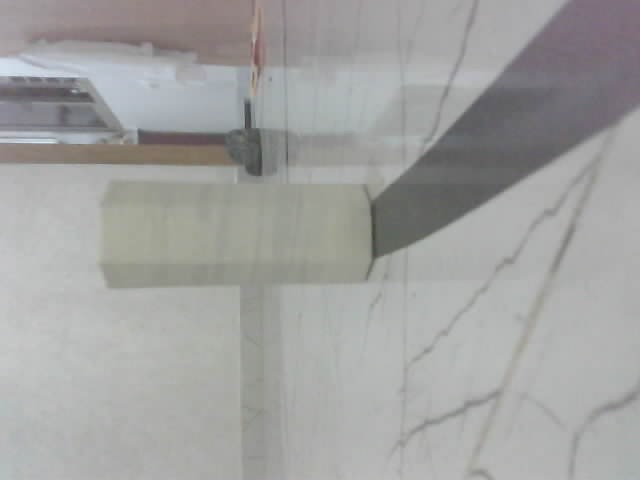
\includegraphics[height=4.6cm]{captures/esp32_brut_tourne.jpg}
  \caption{Image brute (caméra sur la tranche) : aucune détection}
\end{subfigure}\hfill
\begin{subfigure}[b]{0.44\linewidth}\centering
  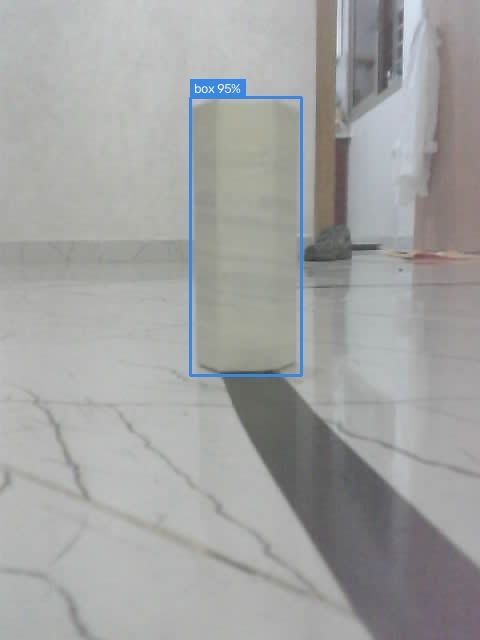
\includegraphics[height=4.6cm]{captures/esp32_detection_box.jpg}
  \caption{Image redressée : boîte détectée à 95\,\%}
\end{subfigure}
\caption{Test du modèle du prototype sur le flux réel de l'ESP32-CAM}
\label{fig:test-reel-proto}
\end{figure}

\subsection{Analyse comparative des deux modèles}
Le tableau~\ref{tab:comparaison} compare les deux modèles entraînés. L'écart de performances s'explique d'abord par
la difficulté des tâches : le modèle routier doit reconnaître des objets très variés dans des milliers de scènes
différentes (villes, météo, éclairage), alors que le modèle du prototype reconnaît deux objets bien définis dans un
environnement contrôlé. Les résultats du modèle routier, obtenus sur des lieux absents de l'entraînement, sont donc
plus représentatifs d'un usage réel ; ceux du prototype mesurent surtout la bonne adaptation au circuit.

\begin{table}[H]
\centering\small
\caption{Comparaison des deux modèles entraînés}
\label{tab:comparaison}
\begin{tabularx}{\linewidth}{l X X}
\toprule
\textbf{Critère} & \textbf{Anomalies routières} & \textbf{Prototype} \\
\midrule
Variante & YOLO26s (\emph{small}) & YOLO26n (\emph{nano}) \\
Données & 7\,894 images réelles, 4 classes & 249 images d'une vidéo + augmentations, 2 classes \\
Entraînement & 8 h, 36 époques & 30 min, 73 époques \\
mAP@50 (test) & 0,526 (temps réel), 0,574 (meilleur réglage) & 0,995 \\
mAP@50-95 (test) & 0,302, 0,346 & 0,976 (0,921 style ESP32) \\
Vitesse sur CPU & 1,4 à 5 images/s (avec le modèle des usagers) & $\approx$ 14 images/s \\
Point fort & généralisation à des lieux inconnus & très fiable sur son circuit \\
Limite & nids-de-poule (rappel 0,25) & domaine étroit, petit test \\
\bottomrule
\end{tabularx}
\end{table}

\chapconclusion
Ce chapitre a présenté la conception des modèles de détection : le choix de YOLO26, la constitution et l'annotation
des données (dont une annotation automatique par SAM~2 pour le prototype), l'entraînement dans un environnement
Docker reproductible, l'exploitation des détections (distance, gravité, priorité) et une évaluation détaillée. Le
modèle routier atteint un mAP@50 de 0,53 en temps réel sur des lieux inconnus, et le modèle du prototype reconnaît
tous les obstacles de son ensemble de test. Le chapitre suivant présente l'application qui exploite ces modèles.

\chapter{Conception et développement de l'application SmartCar Ops}

\chapintro
Ce chapitre présente \app, l'application web de supervision qui réunit les deux autres briques du projet : elle
reçoit les images du prototype et de la caméra embarquée, exécute les modèles de détection, enregistre et priorise
les obstacles, et les met à la disposition de l'opérateur. Nous décrivons d'abord ses objectifs, ses choix
technologiques et son architecture, puis la gestion des données, avant de présenter chacune des huit pages. Nous
terminons par une synthèse des interactions entre les modules.

% =================================================================================================
\section{Présentation générale de l'application}

\subsection{Objectifs et fonctionnalités principales}
\app{} a pour objectif de donner à un opérateur une vue complète et à jour de la situation : où sont les véhicules,
ce qu'ils voient, quels obstacles ont été détectés, lesquels sont les plus dangereux et quel itinéraire les évite.
Ses fonctionnalités principales sont :
\begin{itemize}
  \item la supervision en temps réel de la flotte du monde réel et de la voiture du prototype ;
  \item l'affichage des flux vidéo avec les détections des modèles d'IA superposées ;
  \item l'enregistrement, la fusion, l'évaluation de la gravité et la priorisation des obstacles ;
  \item la planification d'itinéraires qui pondère la distance et le risque ;
  \item des statistiques, la présentation des performances des modèles et la surveillance des équipements ;
  \item le basculement instantané entre les environnements \emph{Monde réel} et \emph{Prototype}.
\end{itemize}

\subsection{Choix de Dash et de Plotly}
L'application est développée en Python avec \textbf{Dash}~\cite{dash}, un framework de Plotly qui permet de construire
des applications web analytiques sans écrire de JavaScript. L'interface est décrite par des composants Python
(convertis en composants React dans le navigateur) et son comportement par des \emph{callbacks} : des fonctions
Python déclenchées lorsqu'une entrée change (clic, sélection, minuterie) et qui mettent à jour des sorties.

Ce choix présente plusieurs avantages pour notre projet :
\begin{itemize}
  \item \textbf{un seul langage} pour l'IA, le traitement d'images (OpenCV~\cite{opencv}, ONNX
        Runtime~\cite{onnxruntime}) et l'interface ;
  \item des \textbf{graphiques interactifs} de qualité grâce à Plotly~\cite{plotly} : cartes routières (MapLibre),
        histogrammes, chronologies, cartes de chaleur ;
  \item le \textbf{multi-pages} intégré (\texttt{use\_pages}) et la bibliothèque \textit{Dash Bootstrap Components}
        pour la mise en page ;
  \item un serveur \textbf{Flask} sous-jacent, que nous utilisons aussi pour relayer le flux vidéo.
\end{itemize}

\subsection{Architecture logicielle de l'application}
L'application est organisée en quatre couches (figure~\ref{fig:archi-logicielle}) :
\begin{itemize}
  \item la couche \textbf{présentation} : \texttt{app.py} construit la structure commune (barre latérale, barre
        supérieure, commutateur d'environnement, minuteries), les modules \texttt{pages/} définissent les huit pages
        et leurs callbacks, et \texttt{components/} regroupe le thème, les composants d'interface et les fonctions
        de création de figures ;
  \item la couche \textbf{métier} (\texttt{core/}) : télémétrie en mémoire (\texttt{hub}), obstacles et gravité,
        graphe routier et planification, trajets, journal d'événements, réglages et accès à la base de données ;
  \item la couche \textbf{services} (\texttt{sources/}) : fils d'exécution d'arrière-plan qui lisent la caméra
        ESP32-CAM et les vidéos, exécutent les détecteurs et font tourner les simulateurs ;
  \item la couche \textbf{données} : base SQLite, instantanés et réglages dans un volume Docker, modèles ONNX et
        leurs profils, graphe routier et plan de la piste.
\end{itemize}
L'ensemble s'exécute dans un conteneur Docker~\cite{docker} : la commande \texttt{docker compose up} suffit pour
lancer l'application sur n'importe quelle machine.

\begin{figure}[H]
\centering
\resizebox{\linewidth}{!}{% Architecture logicielle de SmartCar Ops (chapitre 4)
\begin{tikzpicture}[
  m/.style={bloc,font=\footnotesize,minimum height=1.05cm,text width=#1,minimum width=#1},
  m/.default=3.3cm,
  titre/.style={font=\footnotesize\bfseries,text=#1,anchor=south west,inner sep=1pt}]
  % navigateur
  \node[bloc,draw=gris,fill=gris!8,minimum width=15cm,font=\small] (nav) at (7.5,0.6)
       {Navigateur de l'opérateur — interface Dash (React), rafraîchie par \texttt{dcc.Interval} (1 s et 5 s)};
  % présentation
  \node[m=3.3cm,fill=bleufst!8] (appf) at (2.0,-1.5) {\texttt{app.py}\\structure, menu, commutateur};
  \node[m=3.3cm,fill=bleufst!8] (pages) at (5.7,-1.5) {\texttt{pages/}\\8 pages et leurs callbacks};
  \node[m=3.3cm,fill=bleufst!8] (comp) at (9.4,-1.5) {\texttt{components/}\\thème, panneaux, figures};
  \node[m=3.3cm,fill=bleufst!8] (flask) at (13.1,-1.5) {Serveur Flask\\relais vidéo, instantanés};
  % métier
  \node[m=2.6cm,fill=vertfst!12,draw=vertfst!80!black] (hub) at (1.65,-3.6) {\texttt{hub}\\télémétrie en mémoire};
  \node[m=2.6cm,fill=vertfst!12,draw=vertfst!80!black] (obs) at (4.55,-3.6) {\texttt{obstacles}\\\texttt{severity}};
  \node[m=2.6cm,fill=vertfst!12,draw=vertfst!80!black] (plan) at (7.45,-3.6) {\texttt{planner}, \texttt{network}\\(NetworkX)};
  \node[m=2.6cm,fill=vertfst!12,draw=vertfst!80!black] (trips) at (10.35,-3.6) {\texttt{trips}, \texttt{events}\\\texttt{metrics}};
  \node[m=2.6cm,fill=vertfst!12,draw=vertfst!80!black] (set) at (13.25,-3.6) {\texttt{settings}\\\texttt{db} (SQLite)};
  % services
  \node[m=2.6cm,fill=orangefst!12,draw=orangefst] (cam) at (1.65,-5.7) {\texttt{camera}\\découverte, relais};
  \node[m=2.6cm,fill=orangefst!12,draw=orangefst] (perc) at (4.55,-5.7) {\texttt{perception}\\ArUco, mouvement};
  \node[m=2.6cm,fill=orangefst!12,draw=orangefst] (dash) at (7.45,-5.7) {\texttt{dashcam}\\distance, réaction};
  \node[m=2.6cm,fill=orangefst!12,draw=orangefst] (det) at (10.35,-5.7) {\texttt{detector}\\\texttt{onnx\_yolo}};
  \node[m=2.6cm,fill=orangefst!12,draw=orangefst] (sim) at (13.25,-5.7) {\texttt{sim\_real}\\\texttt{sim\_proto}};
  % données
  \node[m=3.3cm,fill=gris!10,draw=gris] (sqlite) at (2.0,-7.8) {Volume \texttt{/data}\\SQLite, instantanés};
  \node[m=3.3cm,fill=gris!10,draw=gris] (models) at (5.7,-7.8) {\texttt{models/}\\ONNX, profils, registre};
  \node[m=3.3cm,fill=gris!10,draw=gris] (res) at (9.4,-7.8) {\texttt{resources/}\\graphe OSM, piste};
  \node[m=3.3cm,fill=gris!10,draw=gris] (vid) at (13.1,-7.8) {\texttt{demo/videos}\\+ flux ESP32-CAM};
  % couches
  \begin{scope}[on background layer]
    \node[zone,fill=bleufst!4,fit=(appf)(flask)] (z1) {};
    \node[zone,fill=vertfst!5,fit=(hub)(set)] (z2) {};
    \node[zone,fill=orangefst!5,fit=(cam)(sim)] (z3) {};
    \node[zone,fill=gris!5,fit=(sqlite)(vid)] (z4) {};
    \node[draw=encre,thick,rounded corners=8pt,inner sep=8pt,fit=(z1)(z4),
          label={[font=\small\bfseries,anchor=north east]south east:Conteneur Docker \texttt{iot-smartcar-dashboard}}] {};
  \end{scope}
  \node[titre=bleufst] at (z1.north west) {Présentation};
  \node[titre=vertfst!60!black] at (z2.north west) {Métier (\texttt{core/})};
  \node[titre=orangefst!80!black] at (z3.north west) {Services d'arrière-plan (\texttt{sources/})};
  \node[titre=gris] at (z4.north west) {Données};
  \draw[fleche,{Stealth[length=2.6mm]}-{Stealth[length=2.6mm]}] (pages.north |- nav.south) -- (pages.north);
  \draw[fleche] (flask.north) -- (flask.north |- nav.south);
\end{tikzpicture}
}
\caption{Architecture logicielle de \app}
\label{fig:archi-logicielle}
\end{figure}

\subsection{Organisation de l'interface et navigation}
L'interface suit une organisation classique de tableau de bord. À gauche, une barre latérale flottante regroupe les
huit pages par thème (figure~\ref{fig:sidebar}) : \textbf{Live} (Tracking, Camera), \textbf{Planning} (Route
planner), \textbf{Safety} (Obstacles), \textbf{Analytics} (Live stats, AI models) et \textbf{System} (Devices \&
logs), la page \textbf{Overview} étant placée en tête. Une horloge et un voyant d'activité figurent en bas de la
barre. En haut, une barre affiche le titre et la description de la page courante, l'état de la source de données et
le commutateur d'environnement.

\begin{figure}[H]
\centering
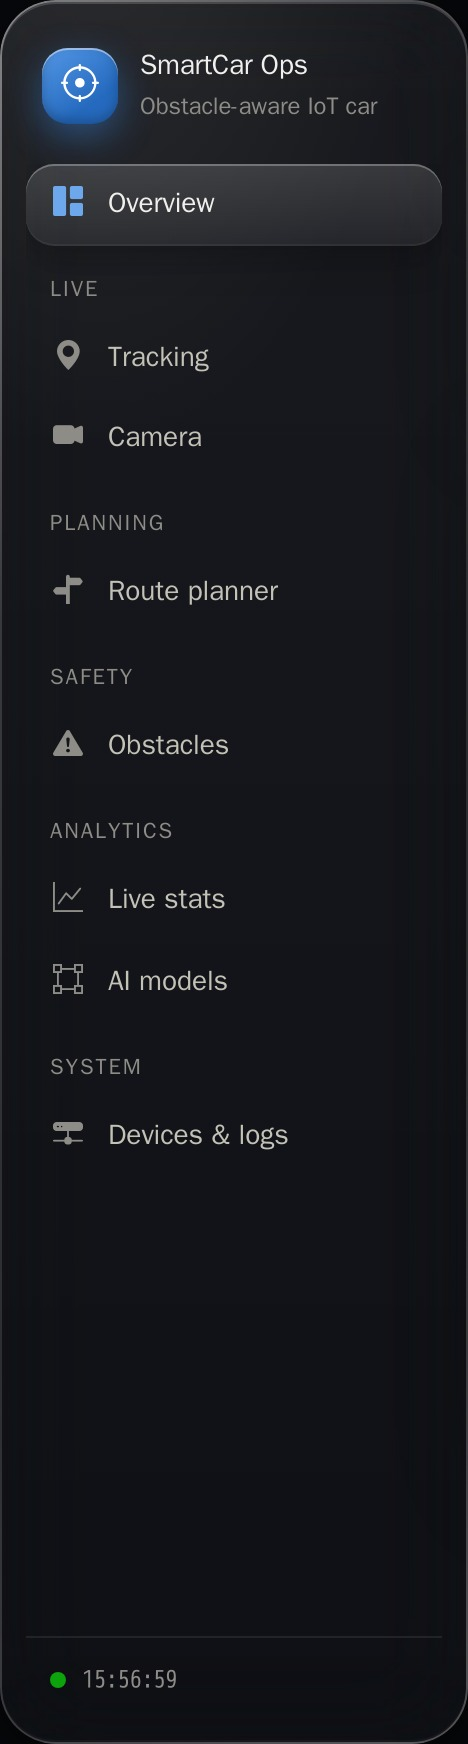
\includegraphics[height=8.6cm]{captures/sidebar.jpg}
\caption{Menu latéral complet de l'application}
\label{fig:sidebar}
\end{figure}

\subsection{Gestion des deux environnements : Real World et Prototype}
Le commutateur de la barre supérieure fait basculer toute l'application entre les deux environnements
(figure~\ref{fig:switch}). Sa valeur est mémorisée dans le navigateur et transmise à chaque callback : chaque page
interroge alors les données de l'environnement choisi et adapte son contenu. Les unités passent des mètres aux
centimètres, la carte routière de Paris laisse place au plan de la piste, et les indicateurs propres à la flotte
(batterie, nombre de véhicules) sont remplacés par ceux du prototype (état de la voiture, progression du parcours,
cadence de la caméra). L'indicateur de source précise l'origine des données : \emph{Simulated data} pour le monde
réel, \emph{Live · ESP32-CAM} lorsque la caméra du prototype est connectée, ou \emph{Demo} lorsqu'elle ne l'est pas.

\begin{figure}[H]
\centering
\begin{subfigure}[b]{\linewidth}\centering
  
\includegraphics[width=\linewidth]{captures/topbar_real.jpg}
  \caption{Environnement \emph{Real-world}}
\end{subfigure}

\vspace{0.2cm}
\begin{subfigure}[b]{\linewidth}\centering
  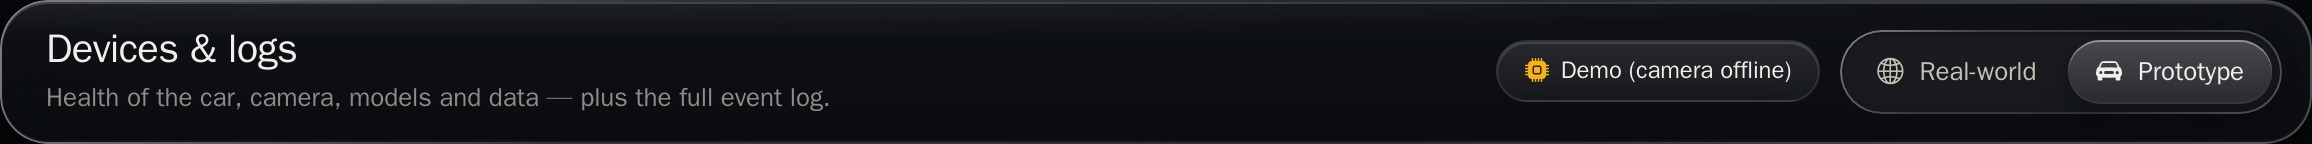
\includegraphics[width=\linewidth]{captures/topbar_proto.jpg}
  \caption{Environnement \emph{Prototype}}
\end{subfigure}

\vspace{0.2cm}
\begin{subfigure}[b]{0.49\linewidth}\centering
  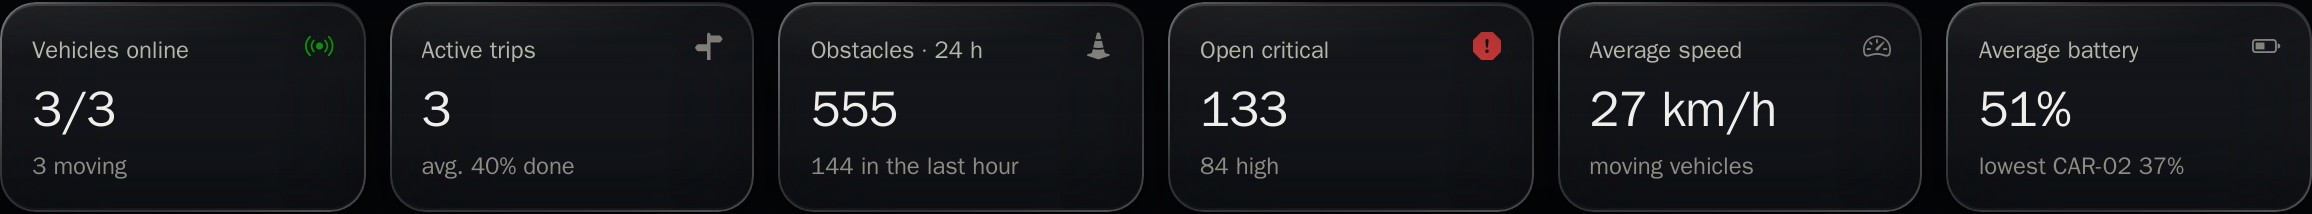
\includegraphics[width=\linewidth]{captures/overview_kpi_real.jpg}
  \caption{Indicateurs de la flotte (monde réel)}
\end{subfigure}\hfill
\begin{subfigure}[b]{0.49\linewidth}\centering
  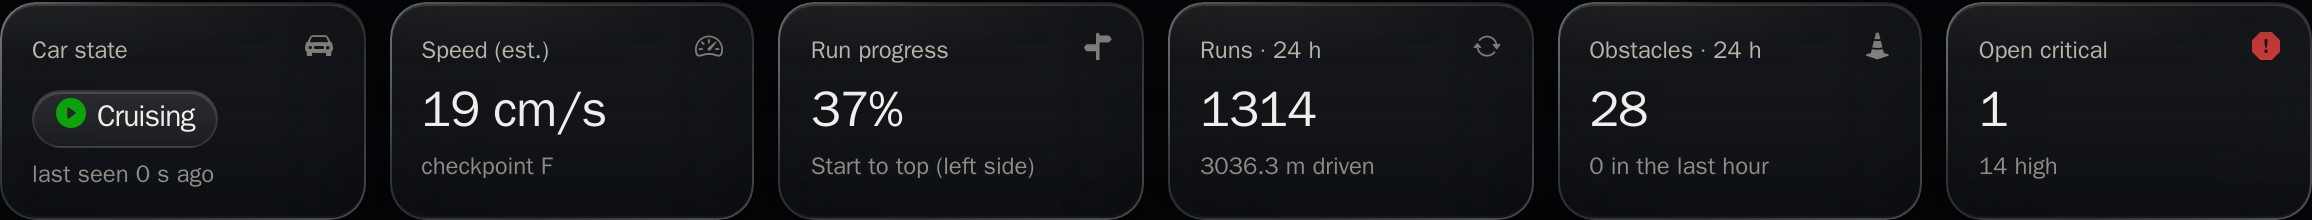
\includegraphics[width=\linewidth]{captures/overview_kpi_proto.jpg}
  \caption{Indicateurs de la voiture (prototype)}
\end{subfigure}
\caption{Changement d'environnement : barre supérieure et indicateurs de la page Overview}
\label{fig:switch}
\end{figure}

% =================================================================================================
\section{Architecture et gestion des données}

\subsection{Architecture générale des échanges de données}
La figure~\ref{fig:flux} décrit la circulation des données. Les \emph{sources} (caméra ESP32-CAM, vidéos de la
caméra embarquée, simulateurs) sont lues par des services qui s'exécutent en arrière-plan, indépendamment des
pages. Les images passent par les détecteurs ; les résultats sont enregistrés dans deux espaces de stockage : un
\textbf{hub en mémoire} pour les données très volatiles (position et état courants des véhicules, dernières
détections) et la \textbf{base SQLite} pour les données à conserver (obstacles, trajets, points de trajectoire,
événements). Les pages lisent ces données à chaque rafraîchissement ; le flux vidéo annoté est servi directement par
le serveur Flask.

\begin{figure}[H]
\centering
\resizebox{\linewidth}{!}{% Flux de données entre les composants (chapitre 4)
\begin{tikzpicture}[
  s/.style={bloc,font=\footnotesize,minimum width=3.0cm,text width=2.8cm,minimum height=1.05cm},
  lb/.style={font=\scriptsize\itshape,text=gris,fill=white,inner sep=1pt},
  col/.style={font=\footnotesize\bfseries,text=gris}]
  % titres de colonnes
  \node[col] at (0,1.15) {Sources}; \node[col] at (4.2,1.15) {Services d'arrière-plan};
  \node[col] at (8.2,1.15) {Modèles}; \node[col] at (12.6,1.15) {Stockage};
  % sources
  \node[s,fill=orangefst!12,draw=orangefst] (esp) at (0,0) {ESP32-CAM\\flux vidéo Wi-Fi};
  \node[s,fill=vertfst!12,draw=vertfst!80!black] (vid) at (0,-1.9) {Vidéos de route\\(dashcam CAR-01)};
  \node[s,fill=gris!8,draw=gris] (sims) at (0,-3.8) {Simulateurs\\(flotte, démo prototype)};
  % services
  \node[s,fill=bleufst!10] (camsvc) at (4.2,0) {Service caméra\\rotation, ArUco, mouvement};
  \node[s,fill=bleufst!10] (dcs) at (4.2,-1.9) {Service dashcam\\distance, voie, réaction};
  % modèles
  \node[s,fill=bleufst!18] (onnx) at (8.2,-0.95) {Détecteurs YOLO26\\(ONNX Runtime)};
  % stockage
  \node[s,fill=gris!10,draw=gris] (hub) at (12.6,0) {Hub en mémoire\\télémétrie, détections};
  \node[s,fill=gris!10,draw=gris] (db) at (12.6,-1.9) {SQLite : obstacles, trajets, événements};
  \node[s,fill=gris!10,draw=gris] (snap) at (12.6,-3.8) {Instantanés JPEG\\(volume \texttt{/data})};
  % consommateurs
  \node[bloc,font=\footnotesize,minimum width=15.6cm,fill=fond] (ui) at (6.3,-5.9)
       {Callbacks Dash (1 s / 5 s) $\rightarrow$ 8 pages \quad | \quad relais MJPEG annoté $\rightarrow$ page Camera
        \quad | \quad planificateur : risque des segments};
  % flux
  \draw[fleche] (esp) -- node[lb,above] {JPEG} (camsvc);
  \draw[fleche] (vid) -- node[lb,above] {images} (dcs);
  \draw[fleche,{Stealth[length=2.4mm]}-{Stealth[length=2.4mm]}] (camsvc.south east) -- node[lb,above,sloped,pos=0.45] {image / boîtes} (onnx.north west);
  \draw[fleche,{Stealth[length=2.4mm]}-{Stealth[length=2.4mm]}] (dcs.north east) -- node[lb,below,sloped,pos=0.45] {image / boîtes} (onnx.south west);
  % bus vers le stockage
  \coordinate (bus) at (10.45,0);
  \draw[very thick,draw=encre] (10.45,0) -- (10.45,-3.8);
  \draw[thick,draw=encre] (camsvc.east) -- node[lb,above,pos=0.55] {position, état, détections} (10.45,0);
  \draw[thick,draw=encre] (dcs.east) -- node[lb,below,pos=0.55] {obstacles, réactions} (10.45,-1.9);
  \draw[thick,draw=encre] (sims.east) -- node[lb,above,pos=0.6] {télémétrie, obstacles simulés} (10.45,-3.8);
  \foreach \n in {hub,db,snap} \draw[fleche] (bus |- \n.west) -- (\n.west);
  % vers l'interface
  \draw[fleche] (hub.east) -- ++(0.35,0) |- ([yshift=0.15cm]ui.east);
  \draw[thick,draw=encre] (db.east) -- ++(0.35,0);
  \draw[fleche] (snap.south) -- (snap.south |- ui.north);
\end{tikzpicture}
}
\caption{Flux des données entre les composants de \app}
\label{fig:flux}
\end{figure}

\subsection{Intégration des modèles YOLO26}
Les modèles sont chargés une seule fois, au démarrage des services, à partir de leurs profils
(chapitre~3) : le service de la caméra embarquée charge les deux modèles routiers, le service de l'ESP32-CAM le
modèle du prototype. L'inférence s'exécute dans un fil dédié qui analyse toujours l'image la plus récente, sans
bloquer ni la lecture vidéo ni l'interface. Les pages n'appellent jamais directement les modèles : elles lisent
leurs résultats dans le hub et la base de données. La page \emph{AI models} affiche les modèles effectivement chargés
et leur temps d'exécution.

\subsection{Acquisition et traitement des données du prototype}
L'Arduino ne disposant d'aucune liaison sans fil, toutes les données du prototype sont extraites de l'image de
l'ESP32-CAM :
\begin{itemize}
  \item \textbf{Découverte de la caméra} : son adresse IP étant dynamique, le service essaie successivement l'adresse
        saisie dans l'application, celle de la configuration, la dernière adresse qui a fonctionné, puis balaye les
        sous-réseaux configurés en testant en parallèle les ports 80 et 81 et la réponse \texttt{/status}.
  \item \textbf{Relais} : la caméra ne servant qu'un client à la fois, le serveur est son unique client et
        redistribue les images à tous les onglets ouverts par la route \texttt{/camera/stream.mjpg}.
  \item \textbf{Redressement} : l'image est tournée selon le montage de la caméra (90° pour notre prototype).
  \item \textbf{Perception} : les marqueurs ArUco~\cite{garrido2014aruco} imprimés aux points de passage A à F
        indiquent à quel point de la piste se trouve la voiture ; entre deux marqueurs, la position est estimée à
        partir de la vitesse mesurée. La différence entre images successives indique si la voiture roule ou est
        arrêtée. Le détecteur fournit les obstacles.
  \item \textbf{Trajets} : le passage au premier marqueur de la trajectoire active ouvre un trajet, le passage au
        dernier le clôture avec la distance parcourue.
\end{itemize}
Lorsque la caméra est hors ligne, un simulateur de démonstration fait rouler une voiture virtuelle sur la piste, afin
que les pages restent utilisables.

\subsection{Gestion des données issues du monde réel}
L'environnement monde réel s'appuie sur le graphe routier du Quartier Latin à Paris, extrait d'OpenStreetMap~\cite{osm}
(309 intersections, 406 tronçons). Un simulateur fait circuler trois véhicules sur ce graphe : il choisit des
trajets, fait avancer les véhicules à des vitesses réalistes, gère leur batterie et produit des rencontres
d'obstacles plus fréquentes sur les tronçons à risque. Le véhicule CAR-01 fait exception : ses obstacles proviennent
uniquement de sa caméra embarquée, alimentée par de vraies vidéos de route (ou un flux réseau, par exemple un
téléphone fixé sur un tableau de bord) et analysée par les modèles. Chaque obstacle statique détecté est placé sur
la carte devant CAR-01, à la distance estimée, et peut le faire ralentir ou s'arrêter.

\subsection{Organisation et stockage des informations}
Les données persistantes sont stockées dans une base \textbf{SQLite}~\cite{sqlite} en mode WAL (journalisation
anticipée, qui permet des lectures pendant les écritures), placée dans un volume Docker. Elle comporte quatre tables :
\begin{itemize}
  \item \texttt{obstacles} : environnement, classe, confiance, proximité, distance, présence sur la trajectoire,
        position, tronçon, score de gravité, niveau, statut (nouveau, acquitté, résolu, faux positif), nombre
        d'observations, dates de première et dernière observation, instantané, source ;
  \item \texttt{trips} et \texttt{trip\_points} : trajets (véhicule, itinéraire, durée, distance, obstacles
        rencontrés) et points de trajectoire horodatés pour la relecture ;
  \item \texttt{events} : journal des événements (niveau, catégorie, message).
\end{itemize}
Les réglages (adresse de la caméra, rotation, trajectoire active, poids de danger) sont conservés dans un petit
fichier JSON, et les instantanés dans un dossier d'images du même volume.

\subsection{Actualisation des données et affichage en temps réel}
Deux minuteries (\texttt{dcc.Interval}) cadencent l'interface : chaque seconde pour les données en direct (positions,
états, détections, indicateurs) et toutes les cinq secondes pour les vues plus lourdes (statistiques, listes). Seuls
les callbacks de la page affichée sont exécutés. La vidéo, elle, n'utilise pas ce mécanisme : la balise image du
navigateur reçoit directement le flux MJPEG relayé, à la cadence de la caméra.

% =================================================================================================
\section{Page Overview : tableau de bord général}

\subsection{Présentation de la vue d'ensemble}
La page \emph{Overview} est la page d'accueil (figure~\ref{fig:overview_real_ecran}). Elle répond en un coup d'œil à
la question « que se passe-t-il maintenant ? » : une rangée d'indicateurs, une carte en direct, une vignette de la
caméra, la liste des obstacles à traiter et les derniers événements.

\capture{overview_real_ecran}{Tableau de bord général (page Overview, environnement monde réel)}

\subsection{Affichage des indicateurs clés}
En environnement monde réel, les indicateurs sont : le nombre d'obstacles critiques ouverts (et d'obstacles de
niveau élevé), le nombre d'obstacles détectés en 24 heures et dans la dernière heure, les véhicules en ligne et en
mouvement, les trajets en cours, la vitesse moyenne et la batterie moyenne de la flotte. En mode prototype, ils
deviennent l'état de la voiture, sa vitesse estimée, la progression du parcours et le nombre de parcours des
dernières 24 heures (figure~\ref{fig:switch}).

\subsection{Synthèse des véhicules et des obstacles}
La carte en direct montre les véhicules, colorés selon leur état (en route, en évitement, arrêté) et les obstacles
ouverts. Le panneau \emph{Needs attention} liste les obstacles ouverts du plus grave au moins grave et le panneau
\emph{Recent events} les derniers événements : arrivée d'un véhicule, obstacle critique, connexion de la caméra…
(figure~\ref{fig:overview-panels}).

\begin{figure}[H]
\centering
\begin{subfigure}[b]{0.49\linewidth}\centering
  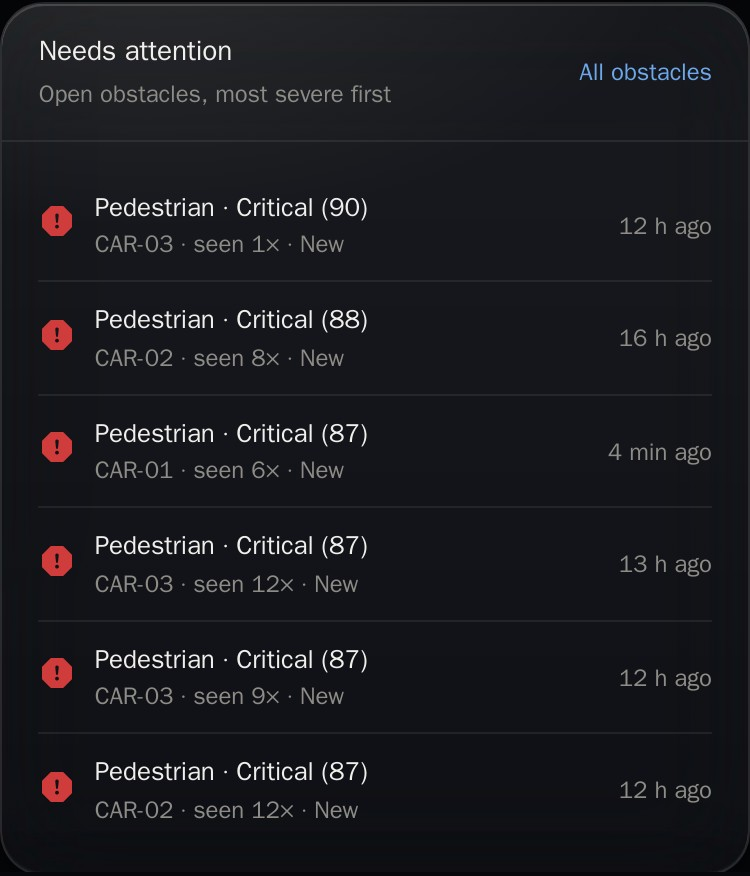
\includegraphics[width=\linewidth]{captures/overview_attention.jpg}
  \caption{Obstacles à traiter}
\end{subfigure}\hfill
\begin{subfigure}[b]{0.49\linewidth}\centering
  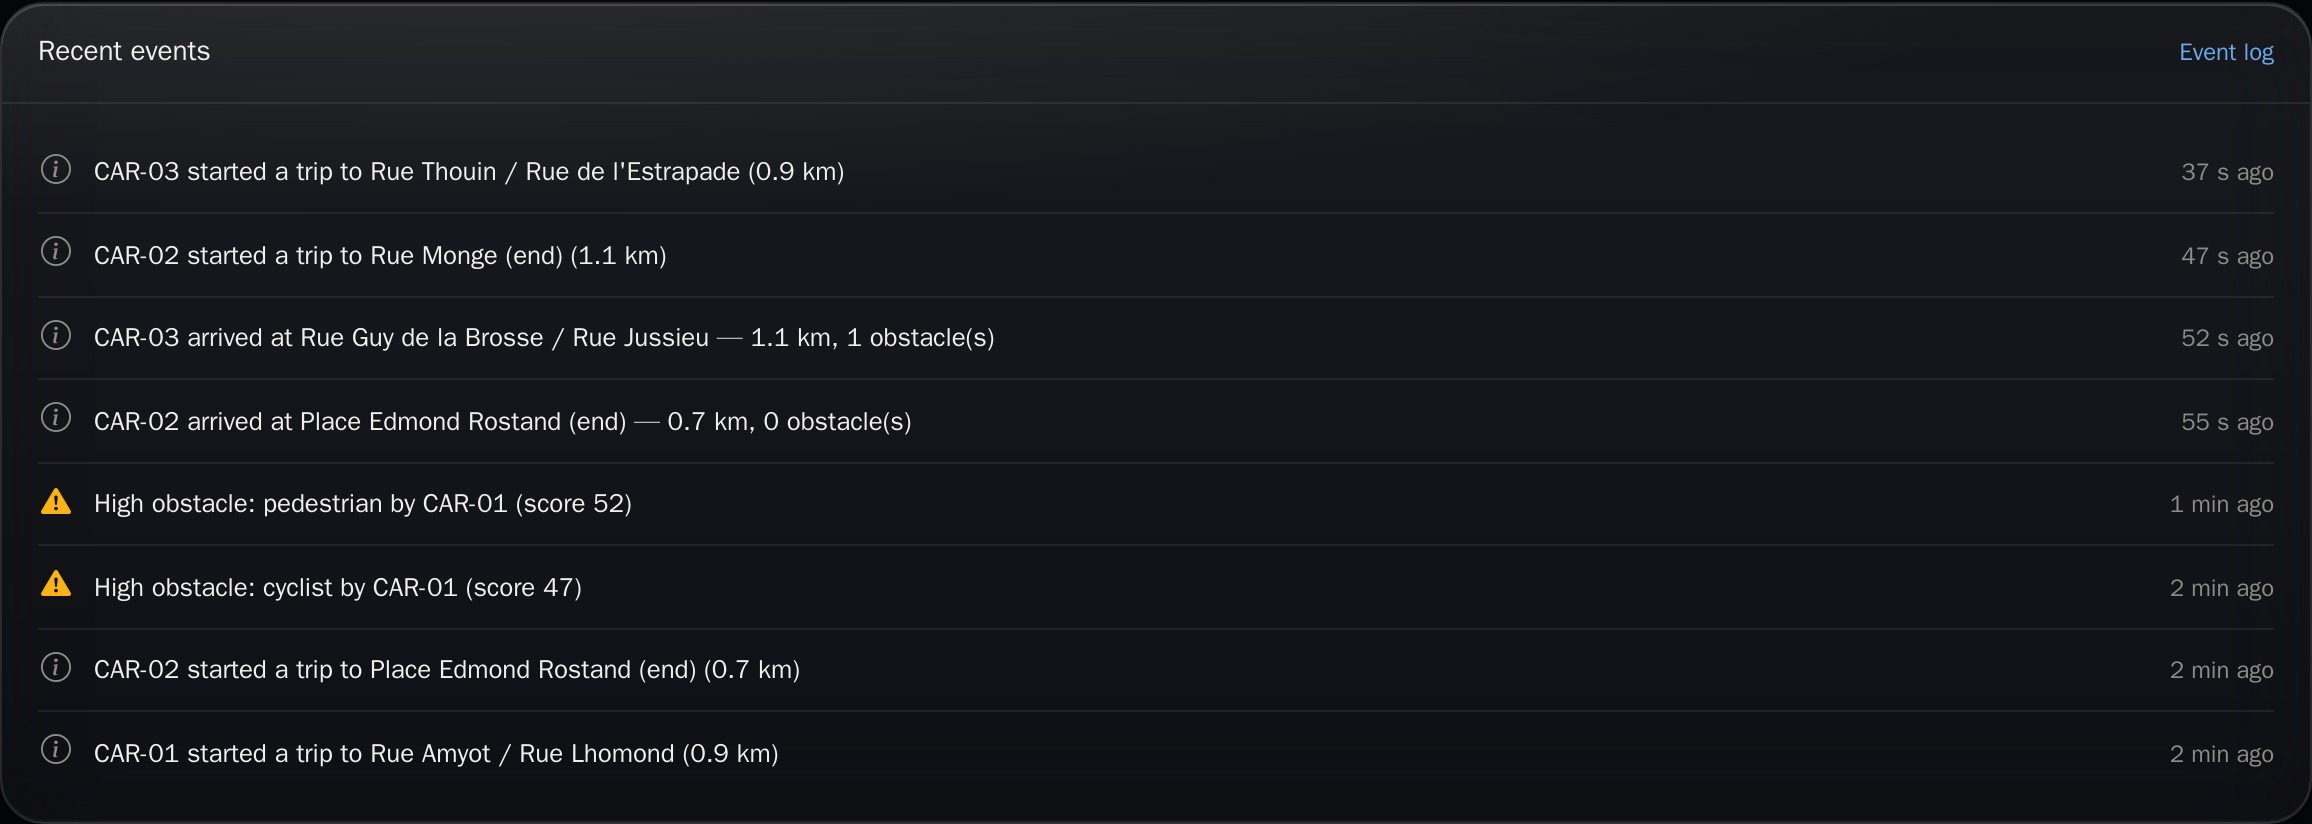
\includegraphics[width=\linewidth]{captures/overview_events.jpg}
  \caption{Événements récents}
\end{subfigure}
\caption{Synthèse des obstacles et des événements de la page Overview}
\label{fig:overview-panels}
\end{figure}

\subsection{Comparaison des environnements Real World et Prototype}
La structure de la page est identique dans les deux environnements, ce qui facilite la prise en main. Seuls le fond
de carte et les indicateurs changent : carte routière et flotte de trois véhicules d'un côté, plan de la piste et
voiture unique de l'autre (figure~\ref{fig:overview-maps}).

\begin{figure}[H]
\centering
\begin{subfigure}[b]{0.49\linewidth}\centering
  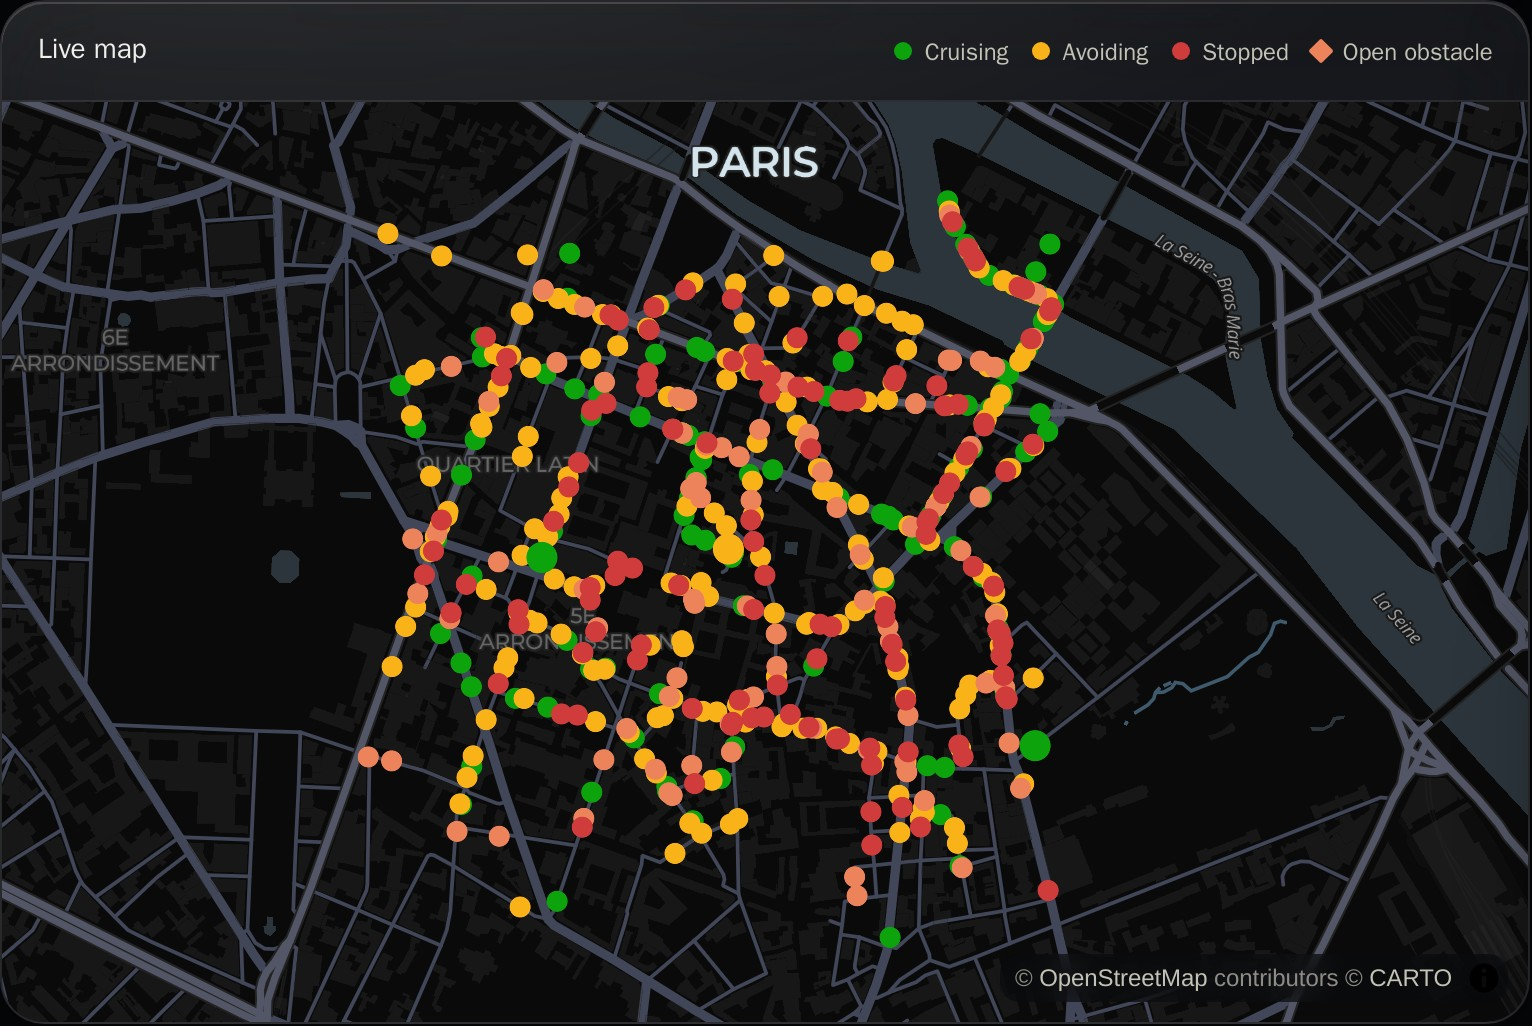
\includegraphics[width=\linewidth]{captures/overview_map_real.jpg}
  \caption{Monde réel : Quartier Latin}
\end{subfigure}\hfill
\begin{subfigure}[b]{0.49\linewidth}\centering
  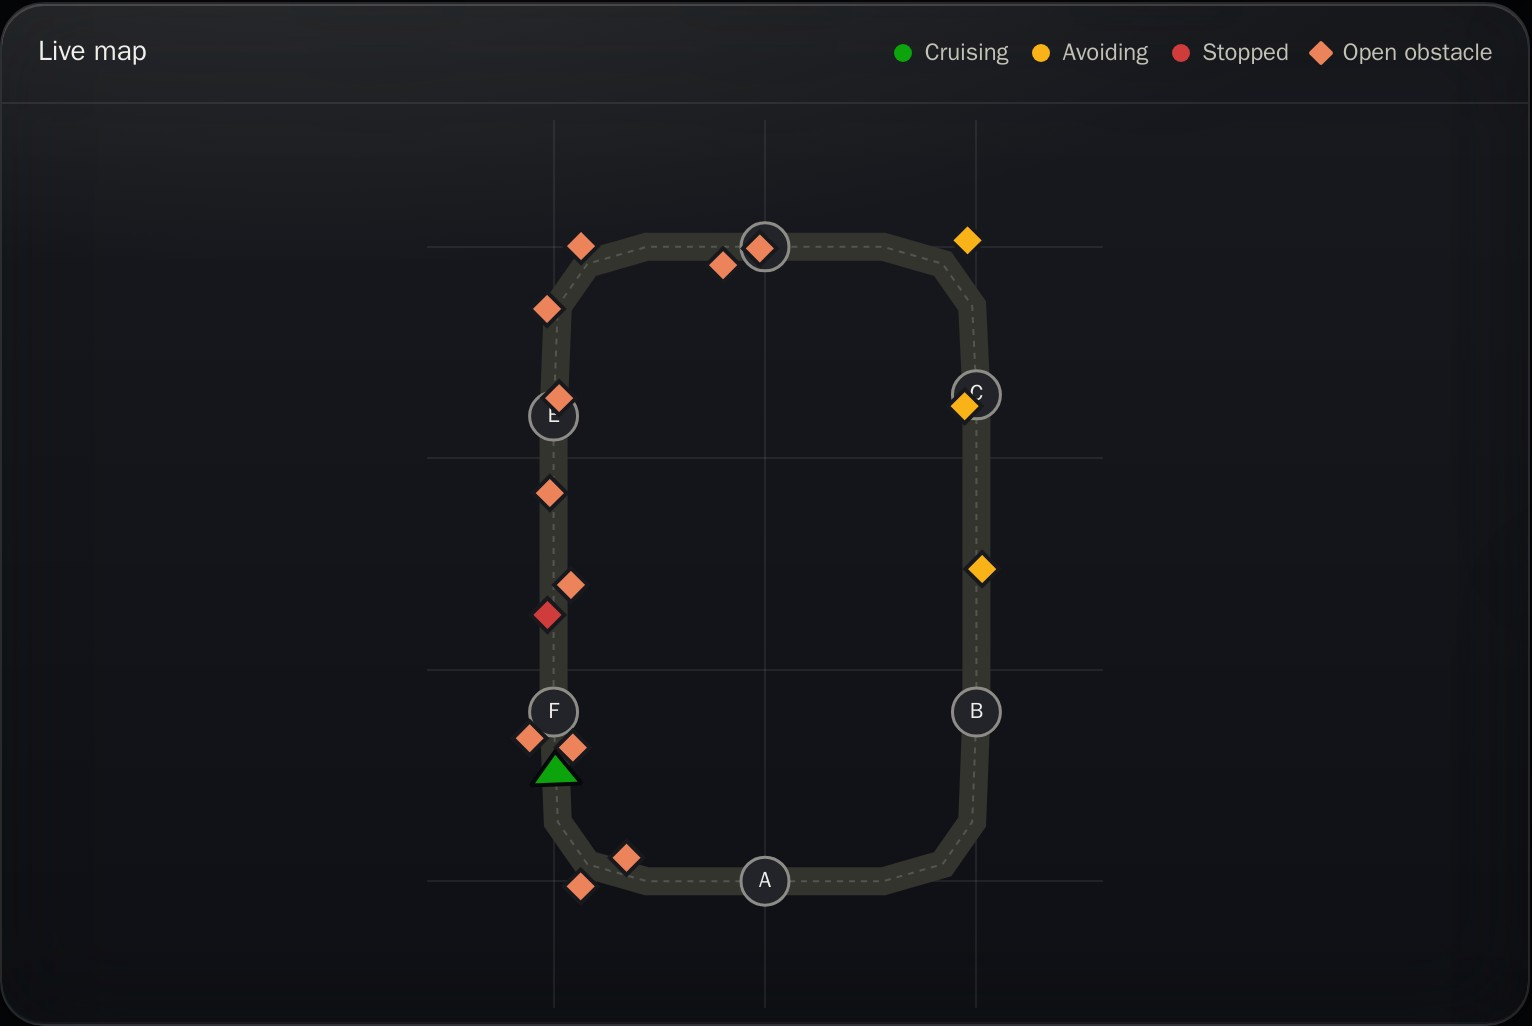
\includegraphics[width=\linewidth]{captures/overview_map_proto.jpg}
  \caption{Prototype : plan de la piste}
\end{subfigure}
\caption{Carte en direct dans les deux environnements}
\label{fig:overview-maps}
\end{figure}

% =================================================================================================
\section{Page Tracking : suivi et localisation des véhicules}

\subsection{Visualisation de la position des véhicules}
La carte de la page \emph{Tracking} affiche la position de chaque véhicule, rafraîchie chaque seconde, avec une
flèche indiquant sa direction (figure~\ref{fig:tracking-map}). Le véhicule sélectionné est mis en évidence. Dans le
prototype, la position est donnée sur le plan de la piste, avec les points de passage A à F.

\begin{figure}[H]
\centering
\begin{subfigure}[b]{0.49\linewidth}\centering
  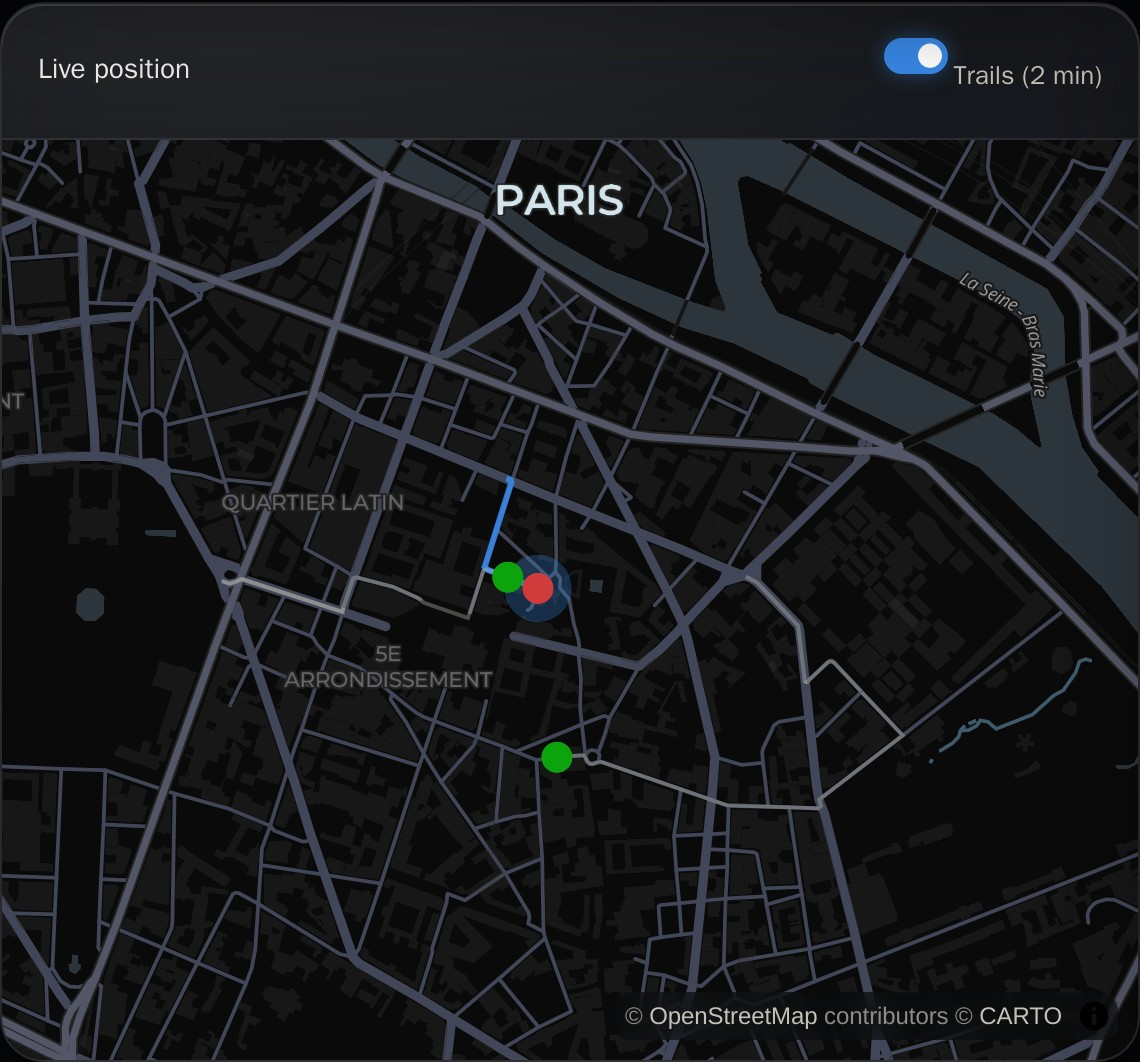
\includegraphics[width=\linewidth]{captures/tracking_map_real.jpg}
  \caption{Monde réel}
\end{subfigure}\hfill
\begin{subfigure}[b]{0.49\linewidth}\centering
  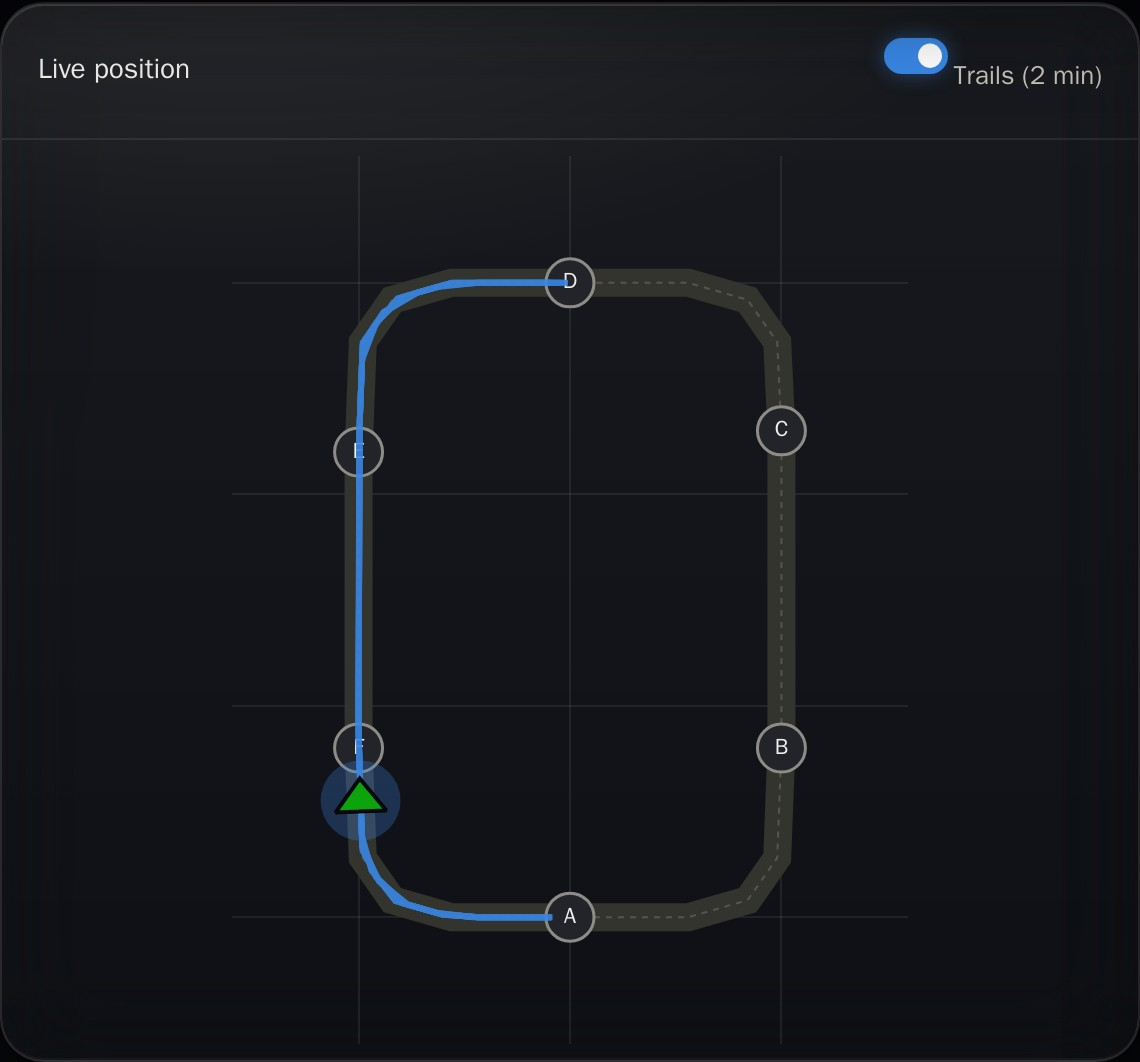
\includegraphics[width=\linewidth]{captures/tracking_map_proto.jpg}
  \caption{Prototype}
\end{subfigure}
\caption{Carte de suivi avec la position des véhicules et leurs traces}
\label{fig:tracking-map}
\end{figure}

\subsection{Suivi des déplacements}
L'option \emph{Trails (2 min)} trace le chemin parcouru par chaque véhicule pendant les deux dernières minutes. La
trace est interrompue à chaque nouveau trajet et lors d'un saut de position (retour de la voiture de démonstration au
départ), pour ne pas dessiner de lignes trompeuses. Le panneau \emph{Vehicles} liste les véhicules en plaçant d'abord
ceux qui posent problème (arrêtés, ligne perdue, en évitement), et le panneau \emph{Selected vehicle} détaille le
véhicule choisi : état, vitesse, batterie, distance à l'obstacle frontal et progression du trajet
(figure~\ref{fig:tracking-panels}).

\begin{figure}[H]
\centering
\begin{subfigure}[b]{0.49\linewidth}\centering
  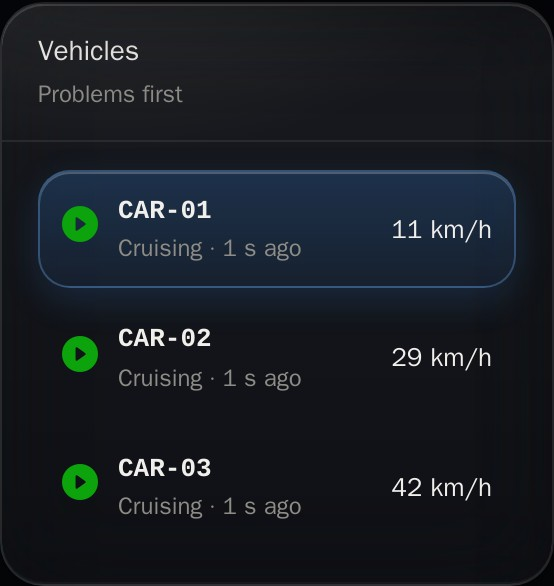
\includegraphics[width=\linewidth]{captures/tracking_vehicles.jpg}
  \caption{Liste des véhicules}
\end{subfigure}\hfill
\begin{subfigure}[b]{0.46\linewidth}\centering
  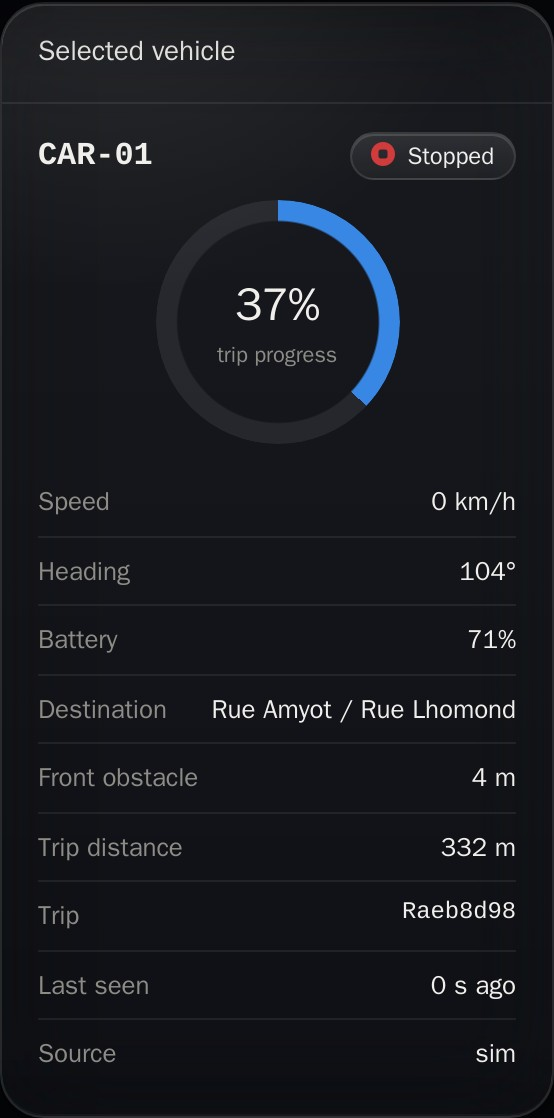
\includegraphics[width=\linewidth]{captures/tracking_selected.jpg}
  \caption{Véhicule sélectionné}
\end{subfigure}
\caption{Suivi des véhicules}
\label{fig:tracking-panels}
\end{figure}

\subsection{Historique des trajectoires}
Chaque trajet est enregistré avec ses points de trajectoire horodatés (position, vitesse, état), échantillonnés
chaque seconde. La table \emph{Trip history} présente les trajets récents : heure de départ, véhicule, itinéraire,
durée, distance et nombre d'obstacles rencontrés.

\subsection{Consultation des parcours précédents}
La sélection d'un trajet dans la table le rejoue sur une carte dédiée : le tracé complet apparaît, un curseur permet
de parcourir le trajet dans le temps et un graphique montre le profil de vitesse (figure~\ref{fig:tracking_history_real}).
Le dernier trajet terminé est sélectionné automatiquement à l'ouverture de la page.

\capture{tracking_history_real}{Historique des trajets et relecture d'un parcours précédent}

\subsection{Gestion des données de localisation}
Les positions courantes sont conservées dans le hub en mémoire (historique glissant pour les traces), alors que
les points de trajectoire des trajets sont écrits dans la base. En monde réel, les coordonnées sont des longitudes et
latitudes et les distances sont calculées en mètres ; dans le prototype, ce sont des coordonnées en centimètres sur le
plan de la piste. Un module de géométrie commun fournit les calculs de distance, de longueur de tracé et
d'interpolation dans les deux systèmes.

% =================================================================================================
\section{Page Camera : visualisation du flux vidéo}

\subsection{Intégration du flux vidéo de l'ESP32-CAM}
En mode prototype, la page affiche le flux de l'ESP32-CAM relayé par le serveur. Le panneau \emph{Connection}
indique l'état de la caméra, son adresse IP et la manière dont elle a été trouvée, la cadence, la résolution, le
détecteur utilisé et le nombre de points de passage reconnus ; il permet de saisir une adresse, de relancer la
recherche sur le réseau, de prendre un instantané et d'\textbf{enregistrer des images} pour enrichir le jeu de données
du prototype. Le panneau \emph{Camera settings} règle la résolution, la qualité JPEG, le flash, le retournement,
le miroir et la \textbf{rotation} de l'image (figure~\ref{fig:camera-proto-panels}).

\begin{figure}[H]
\centering
\begin{subfigure}[b]{0.49\linewidth}\centering
  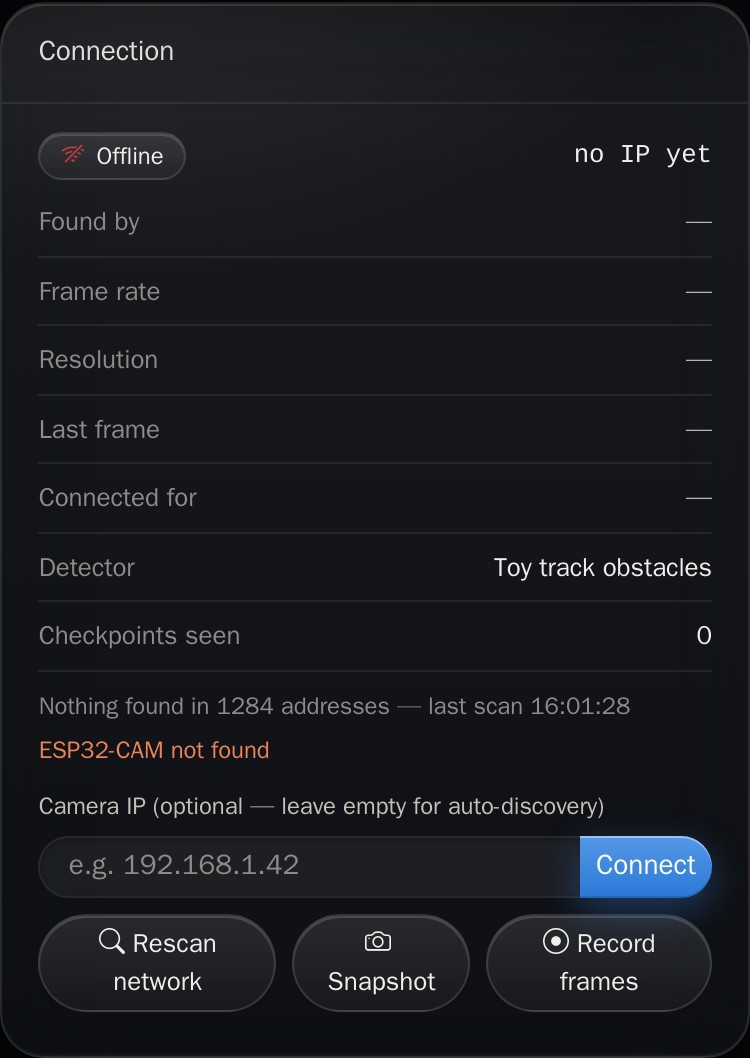
\includegraphics[width=\linewidth]{captures/camera_connection_proto.jpg}
  \caption{Connexion à l'ESP32-CAM}
\end{subfigure}\hfill
\begin{subfigure}[b]{0.49\linewidth}\centering
  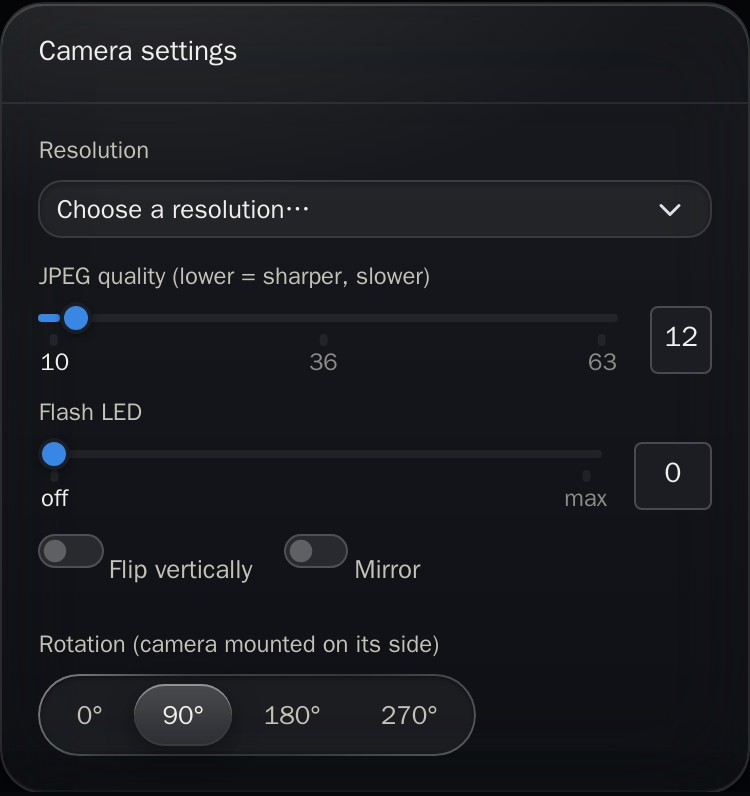
\includegraphics[width=\linewidth]{captures/camera_settings_proto.jpg}
  \caption{Réglages de la caméra}
\end{subfigure}
\caption{Panneaux de connexion et de réglage de l'ESP32-CAM}
\label{fig:camera-proto-panels}
\end{figure}

\subsection{Affichage des images en direct}
L'image est affichée dans un cadre au format de la caméra, surmonté d'un affichage tête haute : indicateur
\emph{LIVE}, cadence, résolution, état de la voiture, point de passage et itinéraire, heure. Un interrupteur
permet d'afficher ou de masquer les détections. Lorsque la caméra est hors ligne, une image d'attente explique la
situation (recherche en cours, dernière adresse connue).

\subsection{Intégration des résultats de l'intelligence artificielle}
Les détections du modèle sont dessinées directement sur l'image relayée : boîte, classe et confiance. En monde
réel, la couleur de la boîte correspond au niveau de gravité et l'étiquette indique aussi la distance estimée
(figure~\ref{fig:camera-ia}).

\begin{figure}[H]
\centering
\begin{subfigure}[b]{0.62\linewidth}\centering
  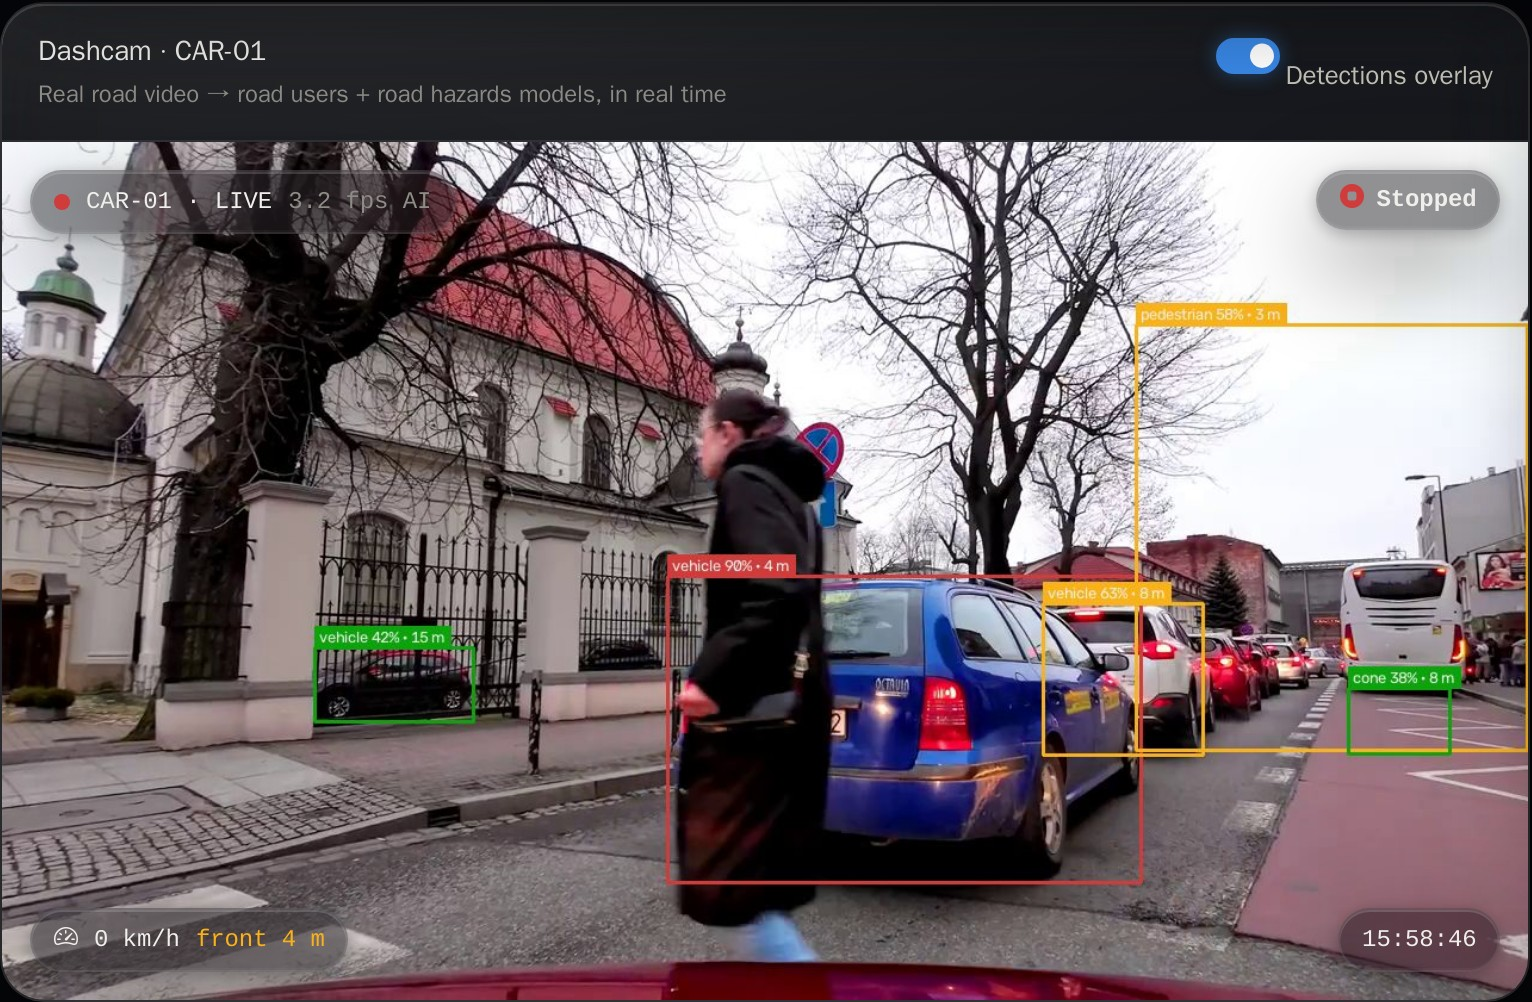
\includegraphics[width=\linewidth]{captures/camera_dashcam.jpg}
  \caption{Monde réel : caméra embarquée de CAR-01}
\end{subfigure}\hfill
\begin{subfigure}[b]{0.36\linewidth}\centering
  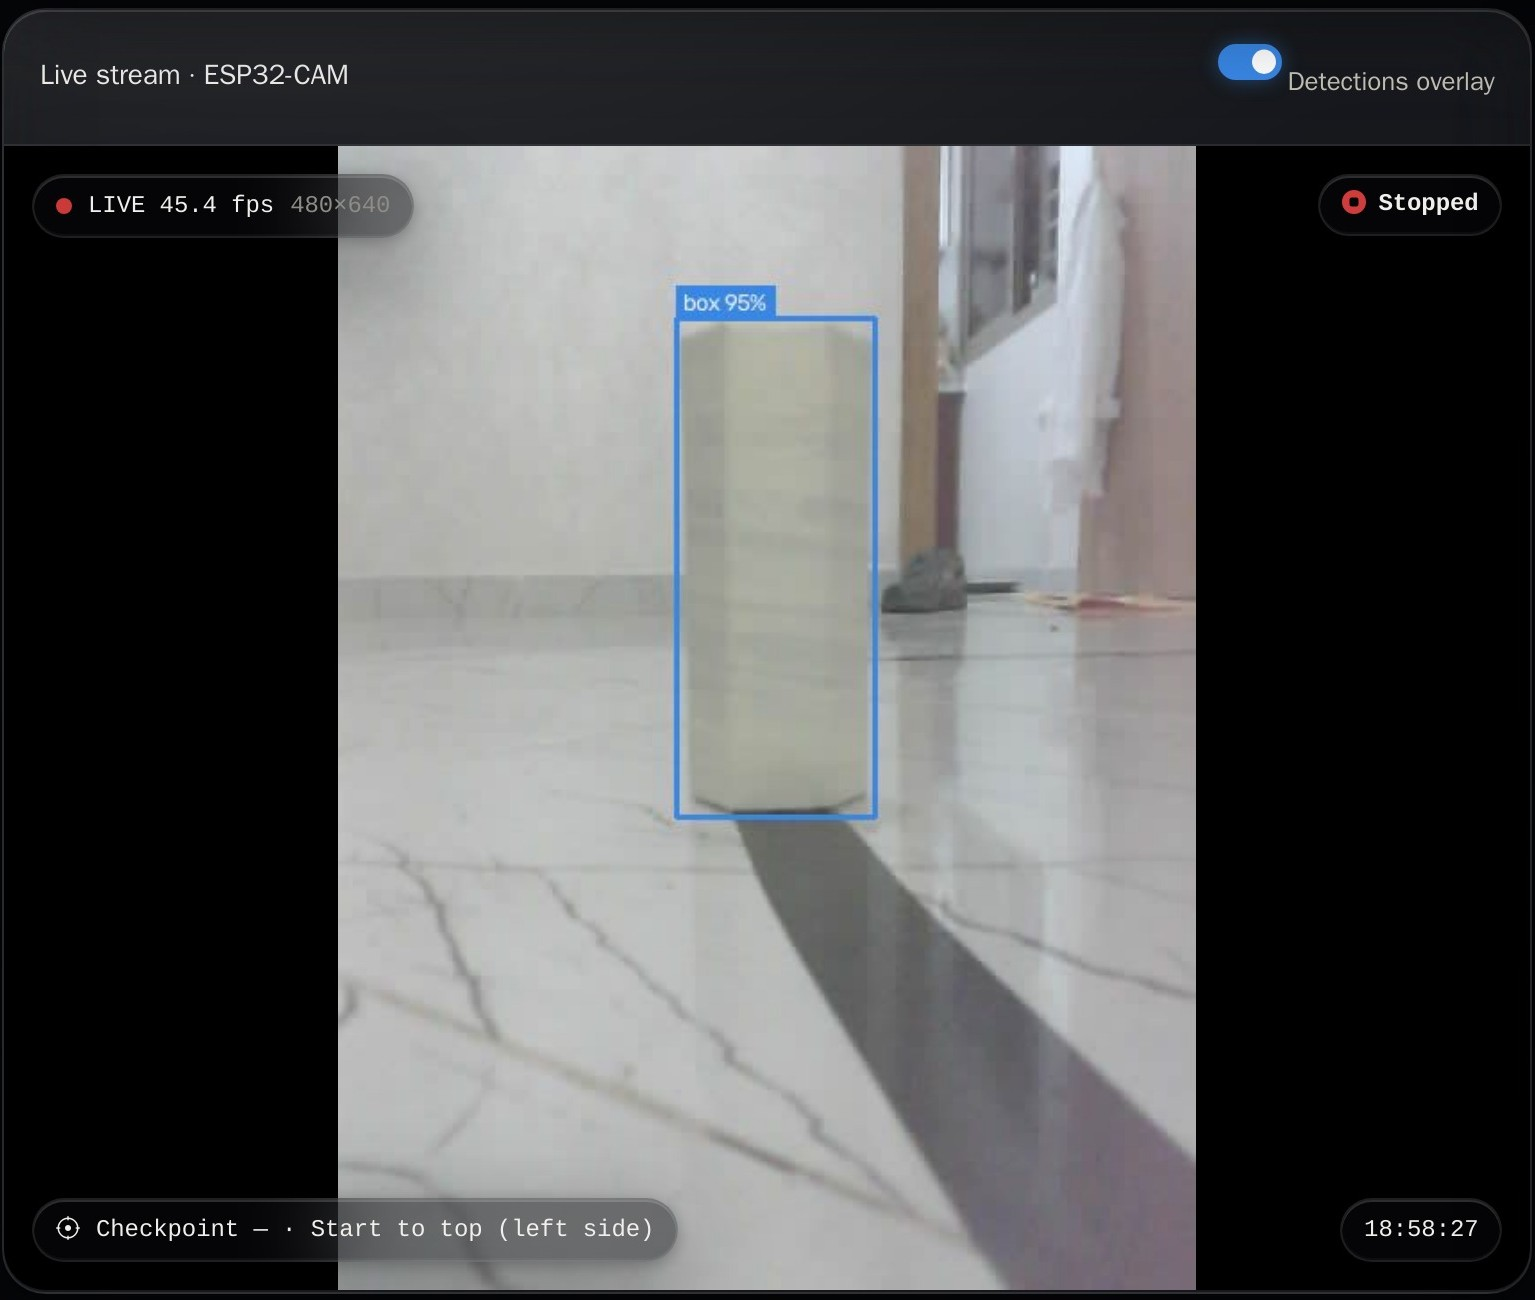
\includegraphics[width=\linewidth]{captures/camera_proto.jpg}
  \caption{Prototype : ESP32-CAM}
\end{subfigure}
\caption{Flux vidéo avec les prédictions des modèles affichées}
\label{fig:camera-ia}
\end{figure}

\subsection{Visualisation des détections sur les images}
Sous la vidéo, le panneau \emph{Live detections} liste les dernières détections (une entrée par classe et par
demi-seconde au plus) avec la confiance, la distance estimée et la position par rapport à la trajectoire ; le
panneau \emph{Models} rappelle les modèles chargés et leur temps d'exécution (figure~\ref{fig:camera-lists}). En mode
prototype, le panneau \emph{Snapshots} rassemble les instantanés enregistrés.

\begin{figure}[H]
\centering
\begin{subfigure}[b]{0.56\linewidth}\centering
  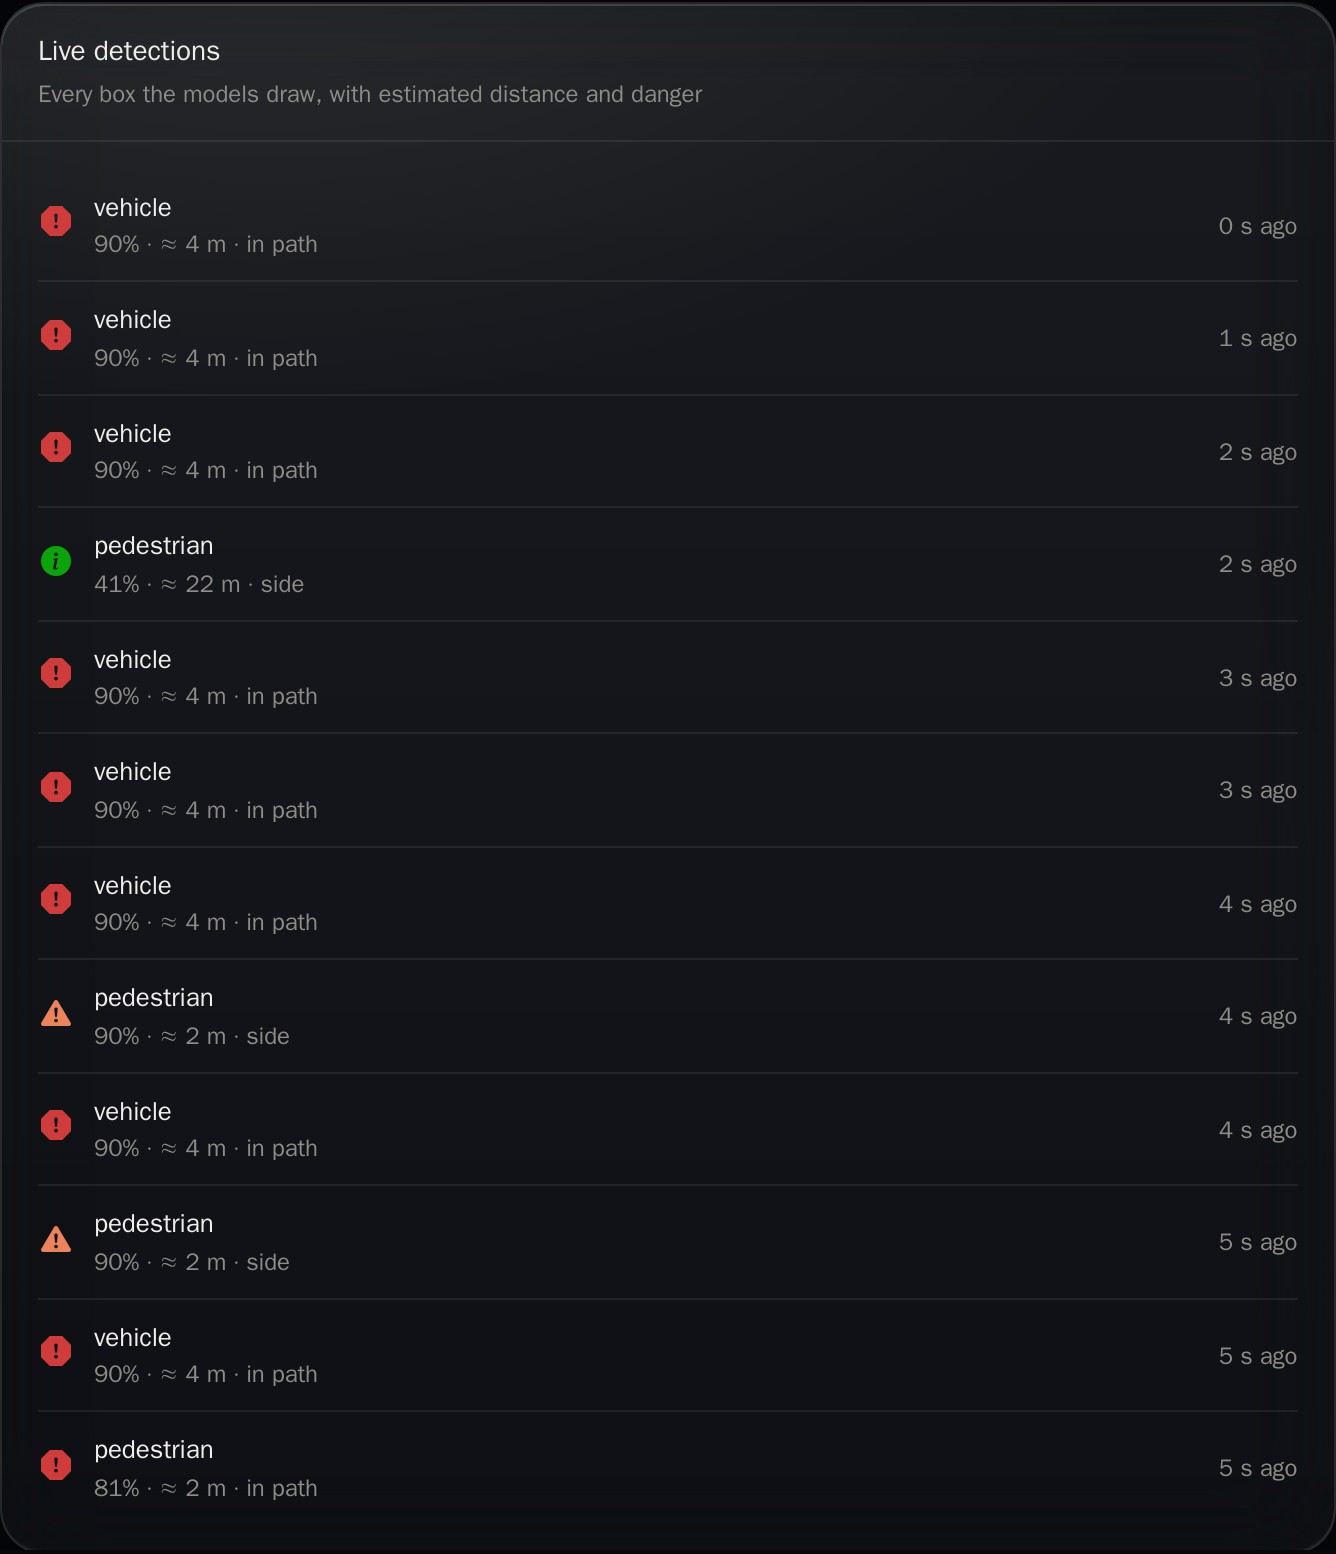
\includegraphics[width=\linewidth]{captures/camera_detections_real.jpg}
  \caption{Dernières détections}
\end{subfigure}\hfill
\begin{subfigure}[b]{0.41\linewidth}\centering
  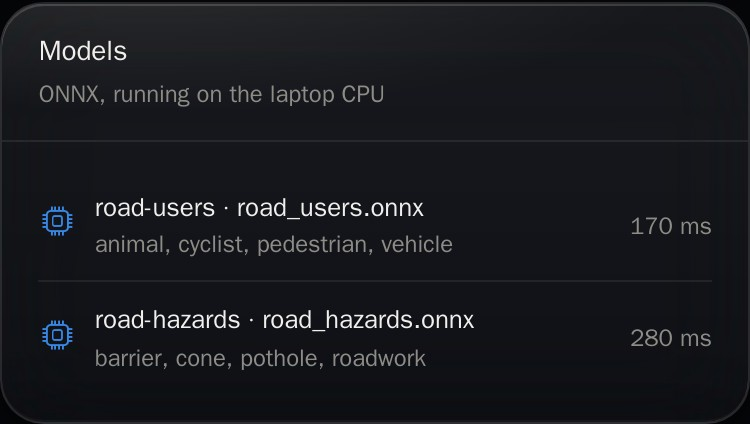
\includegraphics[width=\linewidth]{captures/camera_models_real.jpg}

  \vspace{0.2cm}
  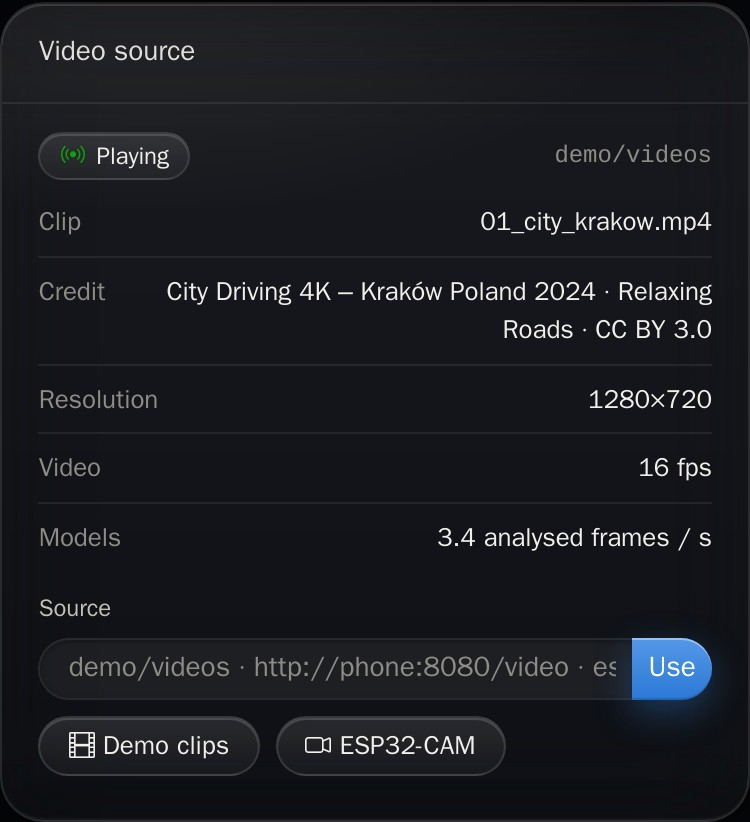
\includegraphics[width=\linewidth]{captures/camera_source_real.jpg}
  \caption{Modèles chargés et source vidéo}
\end{subfigure}
\caption{Détections, modèles et source de la page Camera (monde réel)}
\label{fig:camera-lists}
\end{figure}

\subsection{Comparaison entre les vues Real World et Prototype}
Les deux vues partagent la même logique (relais, détection, affichage tête haute, liste des détections) mais
diffèrent par leur source et leur exploitation. En monde réel, la source est une vidéo de route choisie dans le
panneau \emph{Video source} (clips de démonstration, flux réseau ou ESP32-CAM) et les détections pilotent les
réactions de CAR-01 et la carte des obstacles. En prototype, la source est l'ESP32-CAM de la voiture ; les détections
alimentent la liste des obstacles de la piste et l'état de la voiture.

% =================================================================================================
\section{Page Route Planner : planification des itinéraires}

\subsection{Présentation de l'interface cartographique}
La page \emph{Route planner} associe un formulaire, une carte et une liste d'itinéraires proposés
(figure~\ref{fig:planner_form_real}). La carte affiche le réseau, les obstacles ouverts et, si l'option \emph{Risk
layer} est active, les tronçons à risque colorés selon leur niveau.

\capture[0.6]{planner_form_real}{Formulaire de planification d'itinéraire}

\subsection{Sélection des points de départ et d'arrivée}
Le départ et la destination se choisissent dans des listes d'intersections nommées d'après leurs rues (monde réel)
ou parmi les points de passage de la piste (prototype). Des valeurs par défaut pertinentes sont proposées : deux
intersections éloignées dans le monde réel, le départ et l'arrivée d'une trajectoire de la piste dans le prototype.

\subsection{Représentation des obstacles sur la carte}
Les obstacles ouverts sont représentés par des marqueurs colorés selon leur niveau de gravité ; les tronçons dont le
risque dépasse un seuil sont surlignés en orange (élevé) ou en rouge (critique). Les seuils diffèrent entre les deux
environnements, car la piste, très courte, accumule le risque plus vite.

\subsection{Calcul des itinéraires possibles}
Le réseau est représenté par un graphe : les nœuds sont les intersections (ou points de passage), les arêtes les
tronçons, avec leur géométrie et leur longueur. Les itinéraires sont calculés par l'algorithme de plus court chemin
de Dijkstra~\cite{dijkstra1959} de la bibliothèque NetworkX~\cite{networkx}, avec un coût qui combine distance et
risque.

\subsection{Prise en compte de la distance, des obstacles et de leur gravité}
Chaque tronçon reçoit un \textbf{risque} calculé à partir de l'historique des obstacles qui s'y trouvent :
\begin{equation}
  \text{risque}(e) = \sum_{o \in e} \frac{\text{score}_o}{100} \times w_{\text{statut}} \times
  0{,}5^{\,\text{âge}_o / T_{1/2}}
\end{equation}
Les obstacles graves comptent davantage, les obstacles anciens s'effacent progressivement (demi-vie $T_{1/2}$ de
7 jours dans le monde réel, 2 jours sur la piste), les obstacles résolus ne comptent plus que pour 30\,\% et les faux
positifs sont ignorés. Le coût d'un tronçon est alors :
\begin{equation}
  \text{coût}(e) = \text{longueur}(e) + \alpha \times U \times \text{risque}(e)
\end{equation}
où $U$ exprime la distance qu'« équivaut » une unité de risque (150 m dans le monde réel, 60 cm sur la piste) et
$\alpha$ la priorité choisie par l'opérateur avec le curseur : $\alpha = 0$ donne le plus court chemin, une grande
valeur l'itinéraire le plus sûr.

\subsection{Sélection et affichage de l'itinéraire recommandé}
Trois itinéraires sont calculés : \emph{Recommended} (priorité choisie), \emph{Shortest} ($\alpha = 0$) et
\emph{Safest} ($\alpha = 8$). Lorsque deux d'entre eux coïncident, ils sont fusionnés. L'itinéraire recommandé est
tracé sur la carte avec les obstacles (figure~\ref{fig:planner-route}) ; une phrase résume le compromis, par exemple
« +43 \% de distance par rapport au plus court, 50 \% de risque en moins, évite 35 obstacles ouverts ».

\begin{figure}[H]
\centering
\begin{subfigure}[b]{0.58\linewidth}\centering
  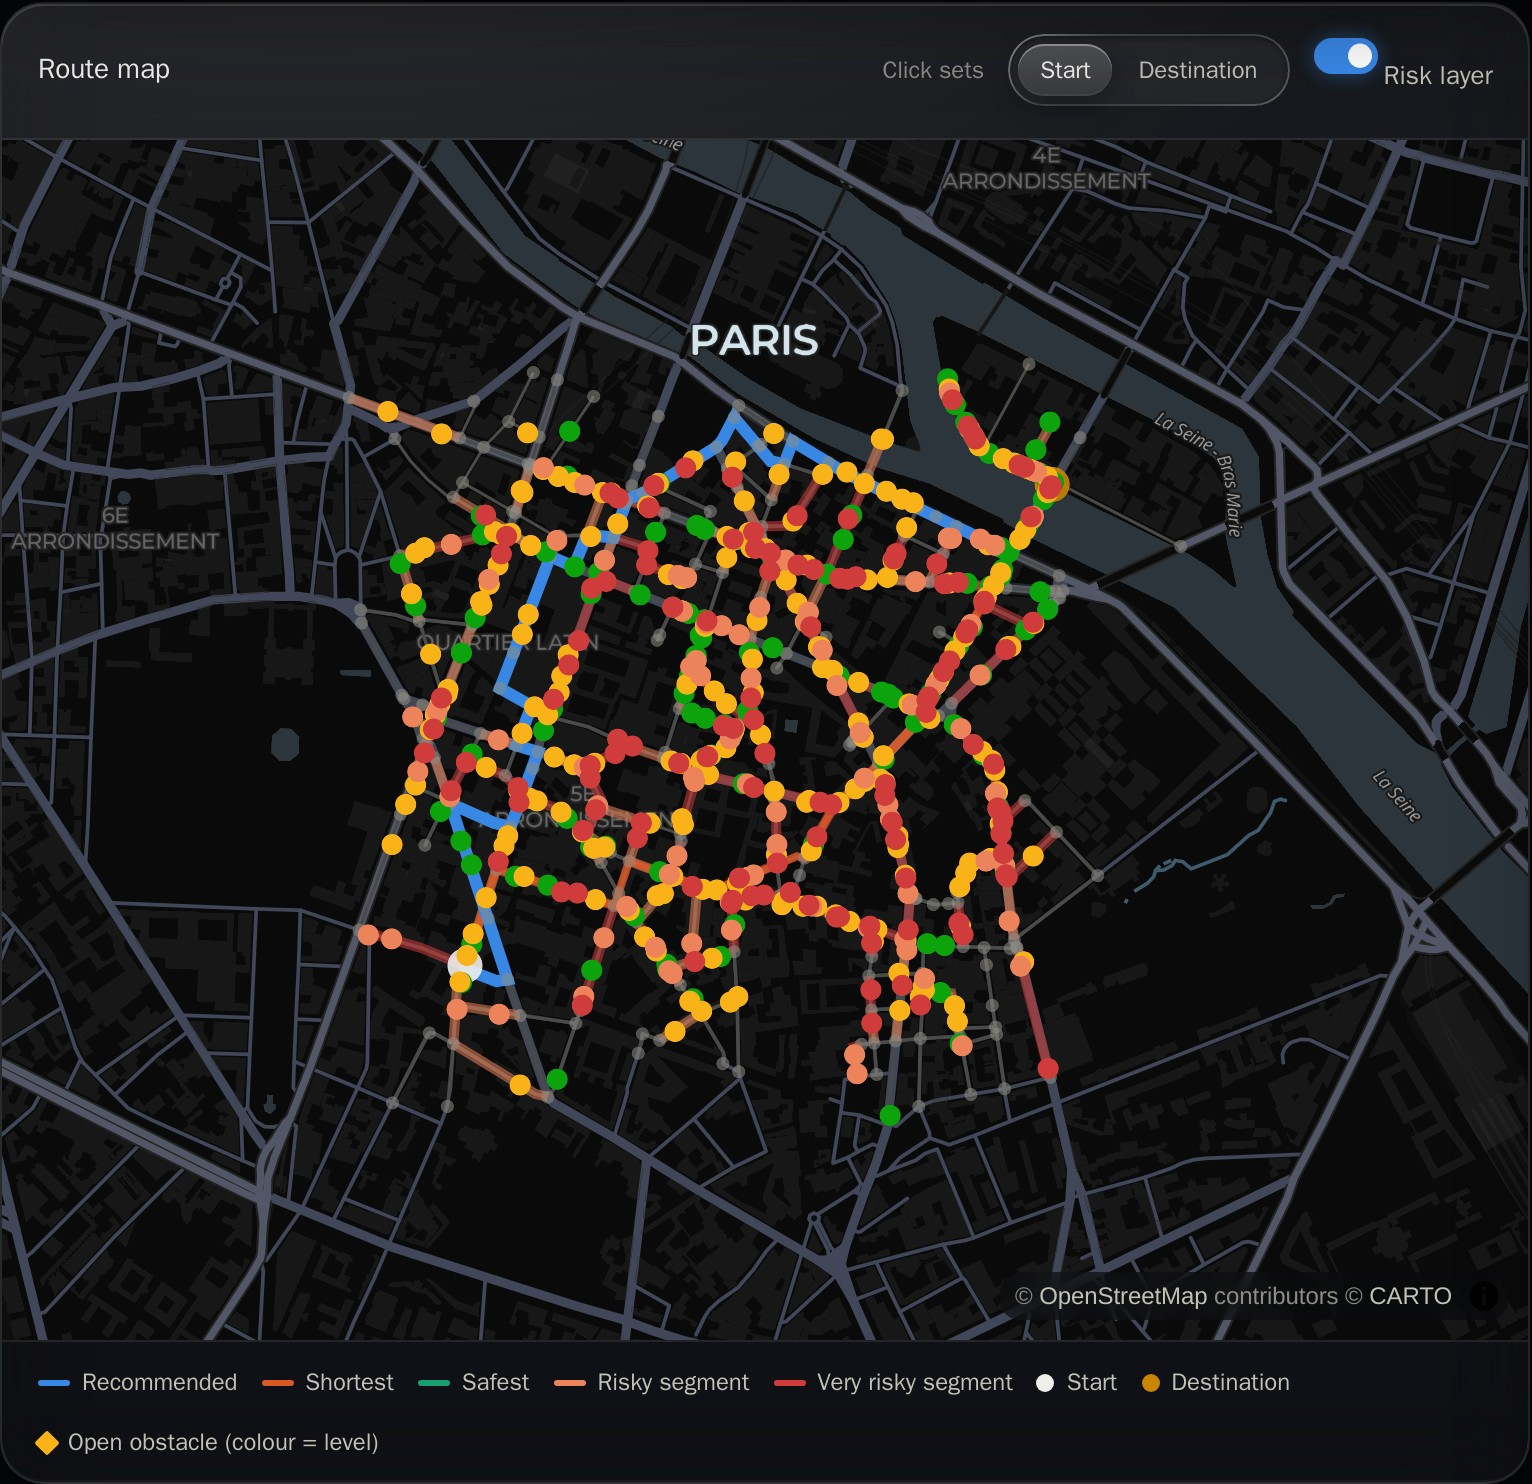
\includegraphics[width=\linewidth]{captures/planner_map_real.jpg}
  \caption{Carte avec l'itinéraire proposé et les obstacles}
\end{subfigure}\hfill
\begin{subfigure}[b]{0.4\linewidth}\centering
  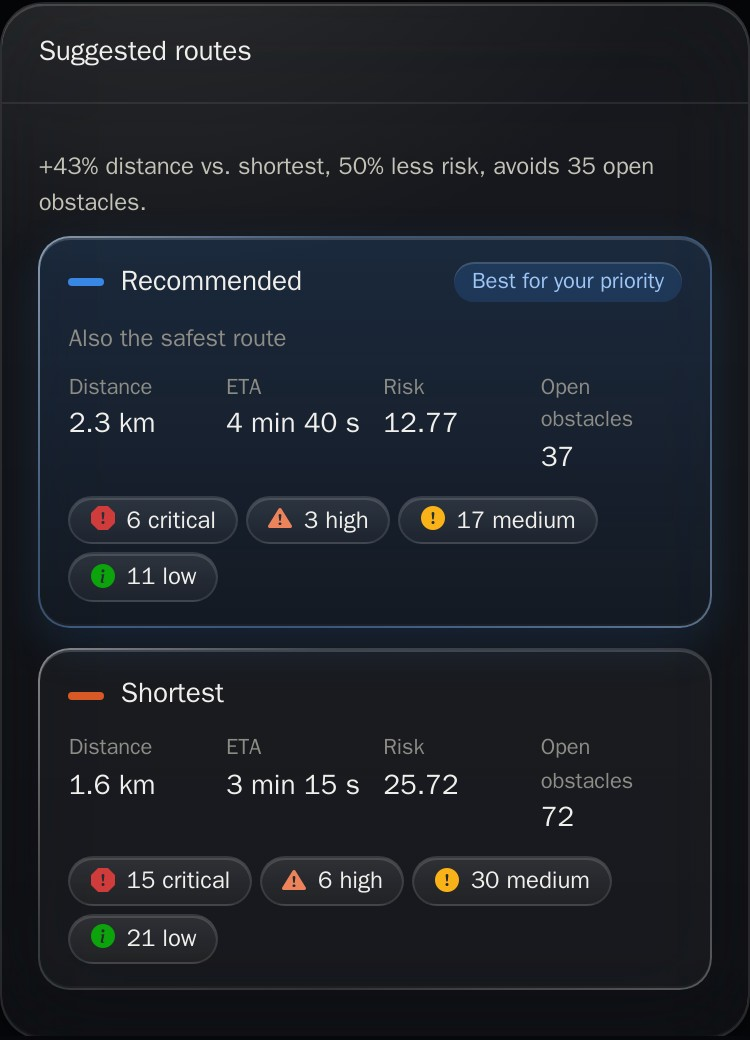
\includegraphics[width=\linewidth]{captures/planner_routes_real.jpg}
  \caption{Itinéraires proposés}
\end{subfigure}
\caption{Itinéraire recommandé, obstacles et tronçons à risque}
\label{fig:planner-route}
\end{figure}

\subsection{Comparaison des itinéraires proposés}
Chaque itinéraire est présenté sur une carte de synthèse avec sa distance, sa durée estimée, son risque cumulé et le
nombre d'obstacles ouverts sur son parcours, répartis par niveau. L'opérateur compare ainsi d'un coup d'œil le gain
de sécurité et le coût en distance. En mode prototype, la page ajoute le classement des \textbf{trajectoires
manuelles} de la piste selon le même coût et un \textbf{éditeur de piste} : positions des points de passage en
centimètres, tronçons, trajectoires, et téléchargement des marqueurs ArUco à imprimer
(figure~\ref{fig:planner-proto}).

\begin{figure}[H]
\centering
\begin{subfigure}[b]{0.49\linewidth}\centering
  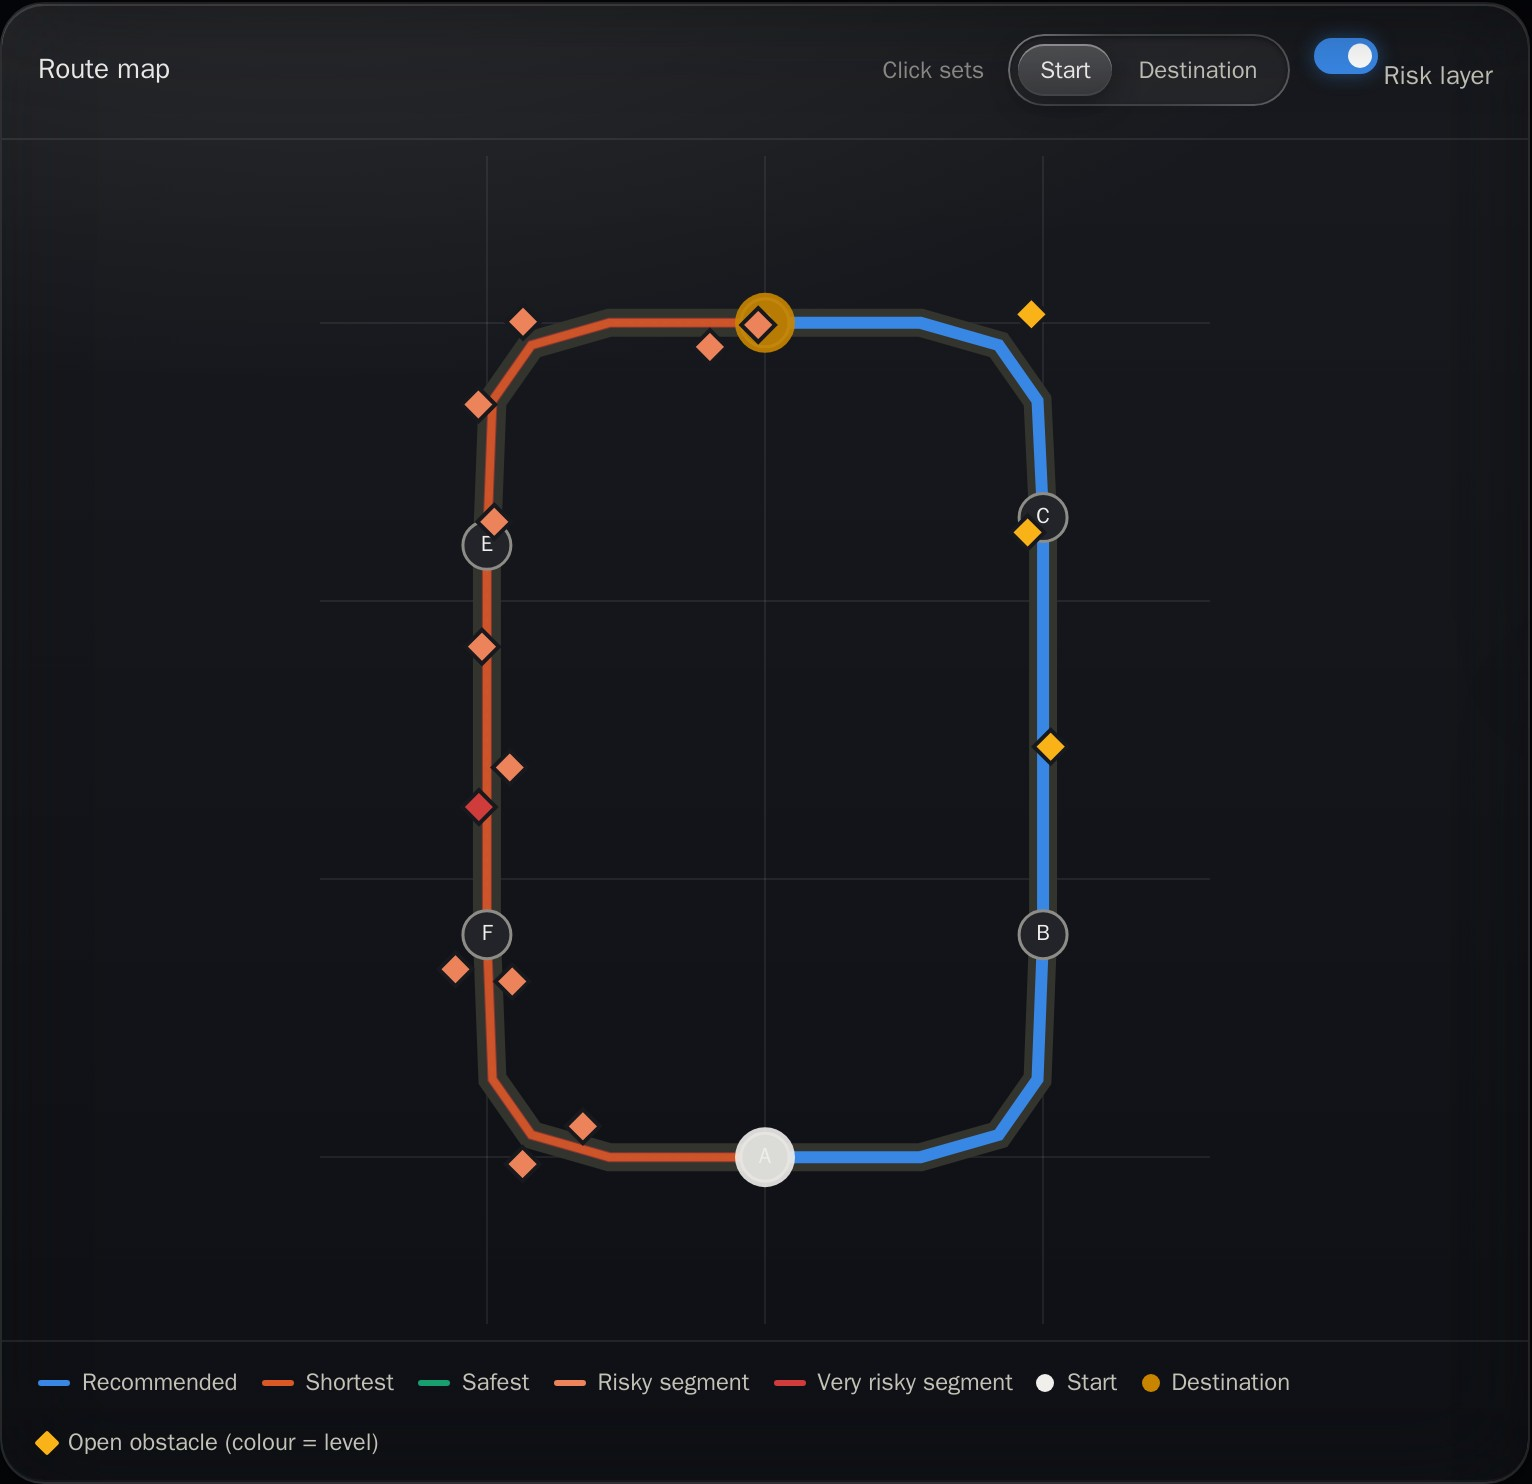
\includegraphics[width=\linewidth]{captures/planner_map_proto.jpg}
  \caption{Carte de la piste}
\end{subfigure}\hfill
\begin{subfigure}[b]{0.49\linewidth}\centering
  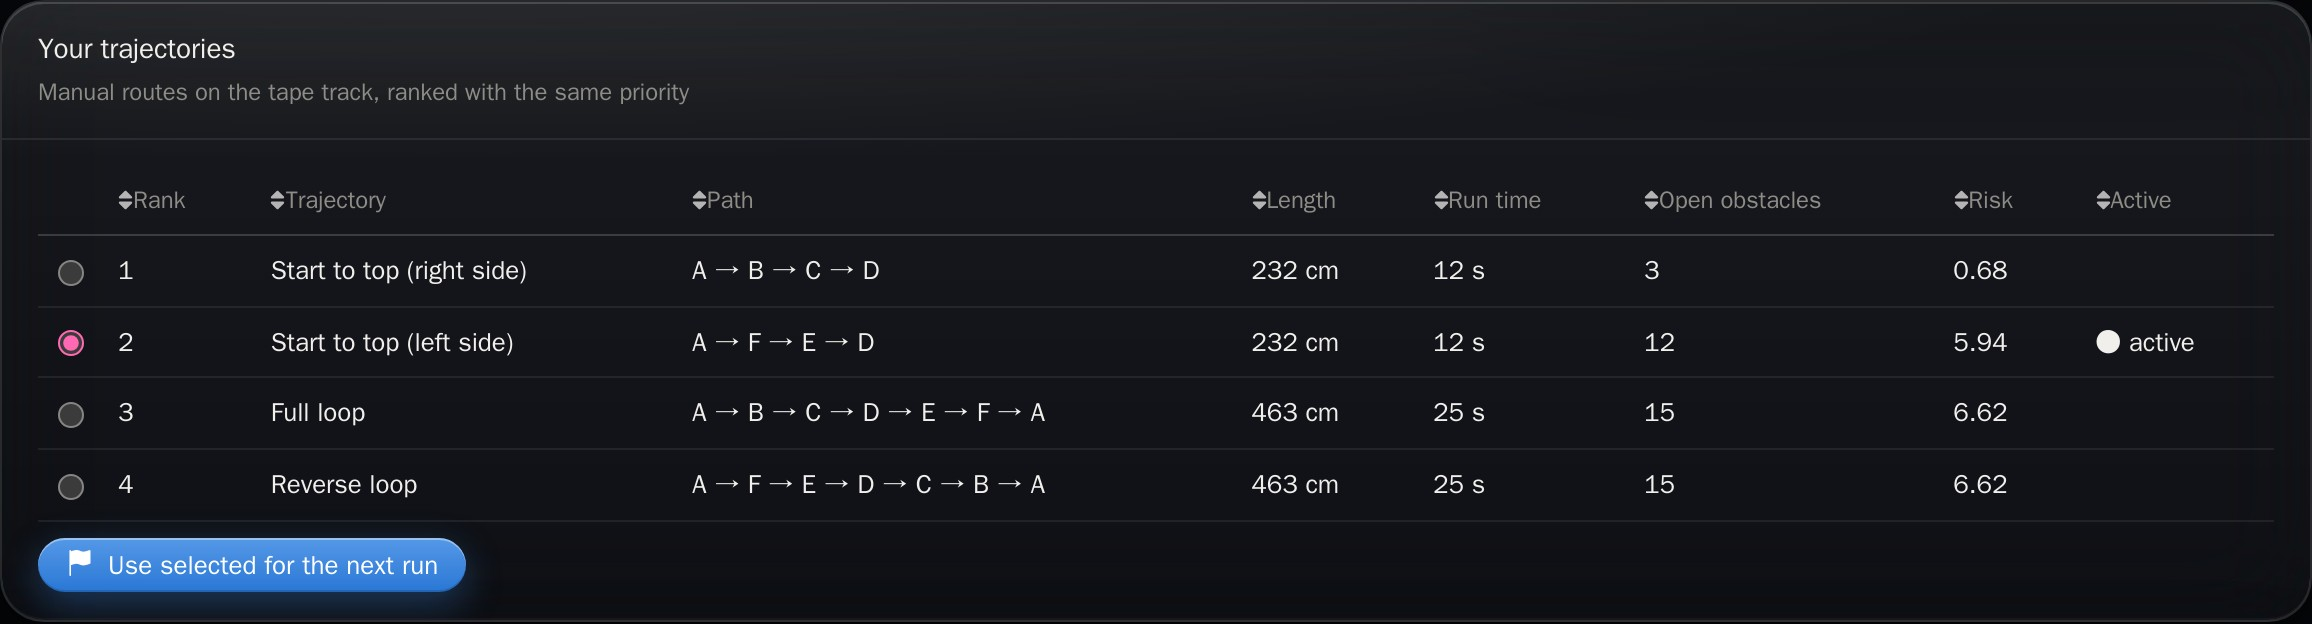
\includegraphics[width=\linewidth]{captures/planner_trajectories_proto.jpg}
  \caption{Trajectoires classées selon la priorité}
\end{subfigure}

\vspace{0.2cm}
\begin{subfigure}[b]{\linewidth}\centering
  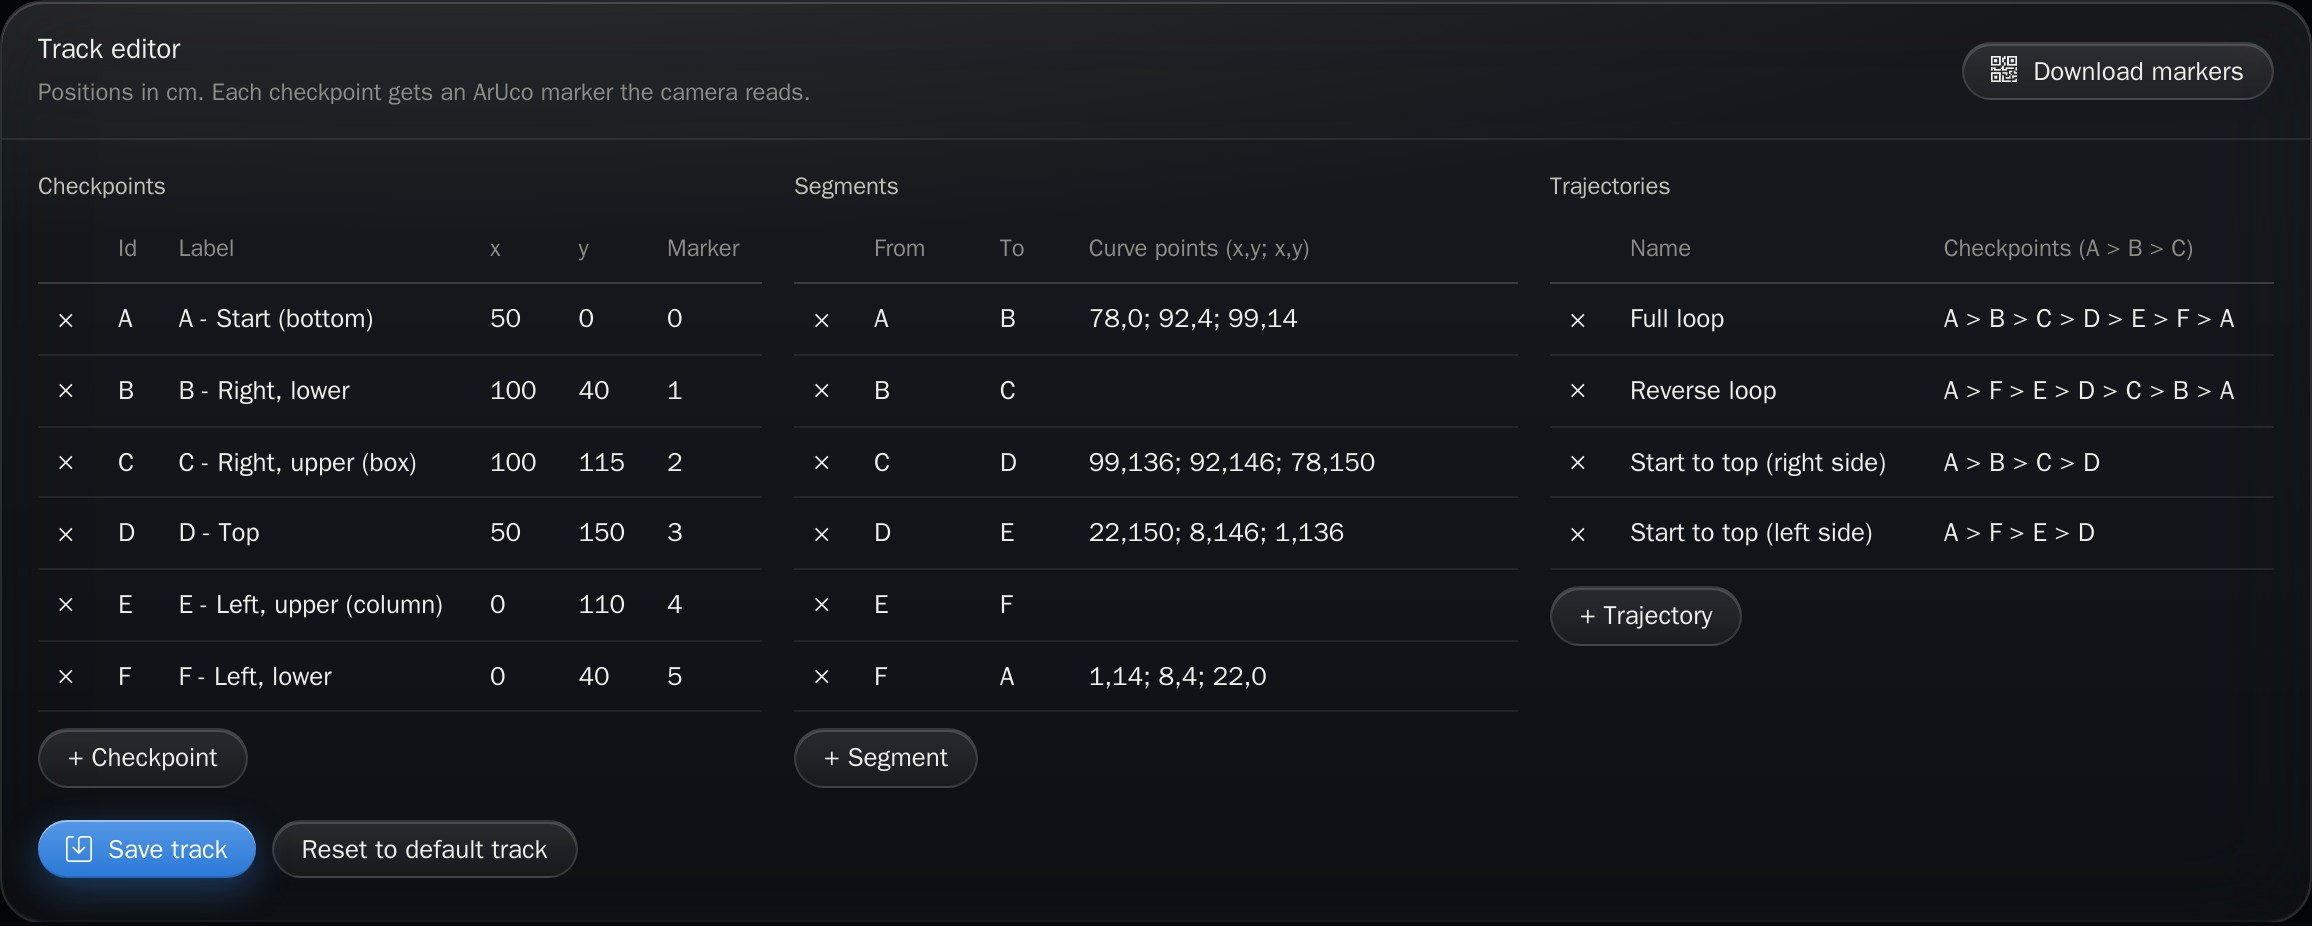
\includegraphics[width=0.8\linewidth]{captures/planner_editor_proto.jpg}
  \caption{Éditeur de piste}
\end{subfigure}
\caption{Planification dans l'environnement prototype}
\label{fig:planner-proto}
\end{figure}

% =================================================================================================
\section{Page Obstacles : gestion et priorisation des anomalies}

La page \emph{Obstacles} est le centre de gestion des anomalies. Elle présente, en haut, une barre de filtres et des
indicateurs, puis la file de priorité, le détail de l'obstacle sélectionné, une carte, une répartition par classe et
par niveau, et une explication du calcul de la priorité (figure~\ref{fig:obstacles_queue}).

\capture{obstacles_queue}{Liste des anomalies détectées, triées par priorité}

\subsection{Affichage des obstacles détectés}
La file de priorité est une table paginée qui présente pour chaque obstacle : son niveau, son score, la classe, la
confiance, la distance estimée, sa position sur la trajectoire ou sur le côté, le nombre d'observations, la date de la
dernière observation, le statut et le véhicule qui l'a détecté. Les obstacles vus plusieurs fois n'apparaissent
qu'une fois, avec leur compteur d'observations.

\subsection{Identification des nids-de-poule et autres anomalies}
Les anomalies proviennent de deux sources : les détections réelles des modèles (caméra embarquée de CAR-01 et
ESP32-CAM du prototype), accompagnées d'un instantané annoté, et les rencontres produites par le simulateur pour
les autres véhicules de la flotte, signalées comme simulées. Le détail de l'obstacle précise sa source.

\subsection{Classification des obstacles par catégorie}
Chaque obstacle porte l'une des classes du vocabulaire commun : piéton, cycliste, animal, véhicule, nid-de-poule,
cône, barrière, panneau de chantier, débris, et, pour le prototype, colonne et boîte. Un filtre permet de n'afficher
que certaines classes, et le graphique \emph{By object and level} montre leur répartition
(figure~\ref{fig:obstacles-repartition}).

\begin{figure}[H]
\centering
\begin{subfigure}[b]{0.49\linewidth}\centering
  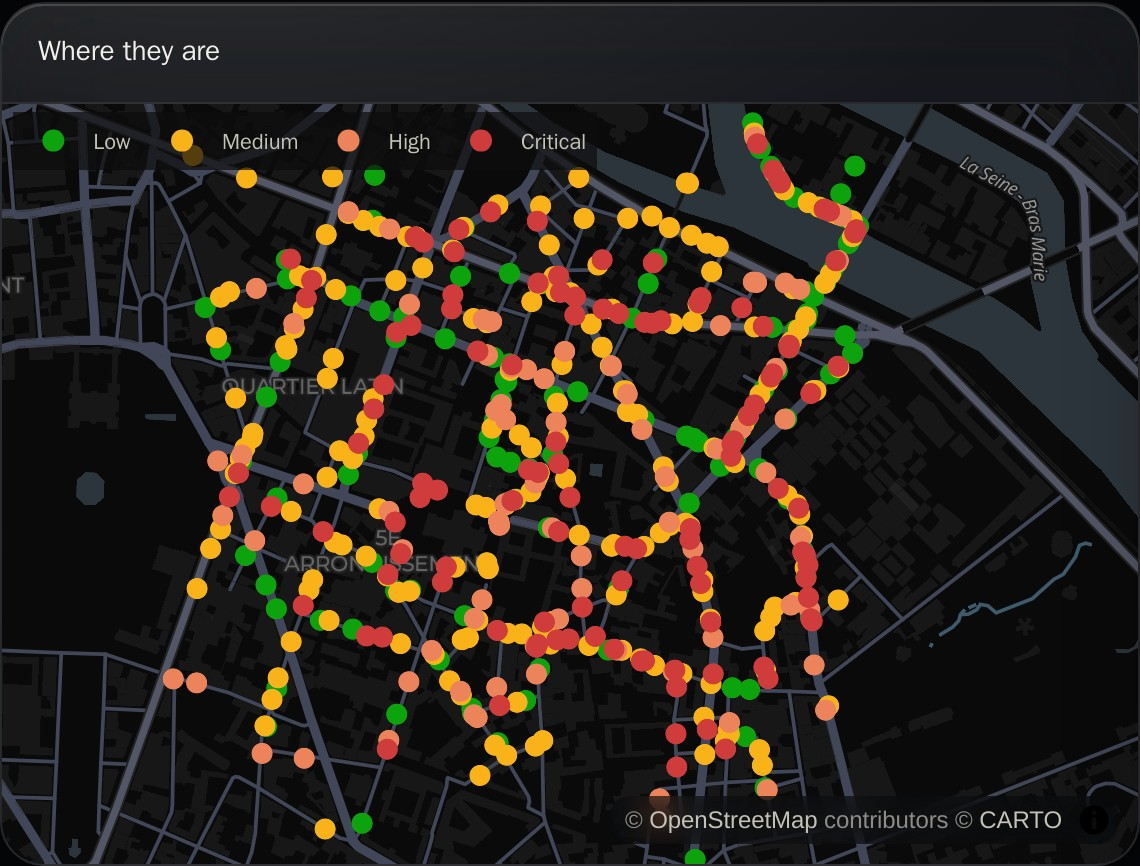
\includegraphics[width=\linewidth]{captures/obstacles_map.jpg}
  \caption{Localisation des obstacles par niveau}
\end{subfigure}\hfill
\begin{subfigure}[b]{0.49\linewidth}\centering
  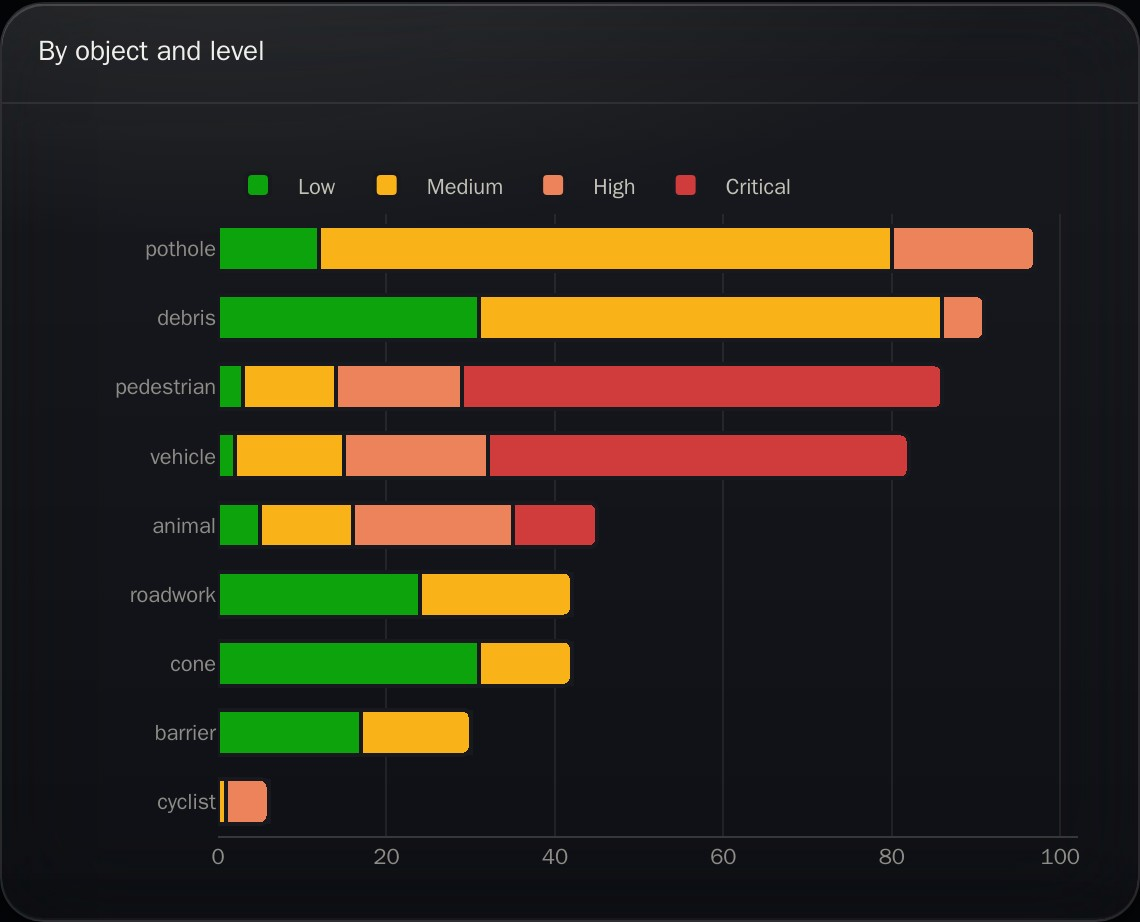
\includegraphics[width=\linewidth]{captures/obstacles_bars.jpg}
  \caption{Répartition par classe et par niveau}
\end{subfigure}
\caption{Carte et répartition des obstacles}
\label{fig:obstacles-repartition}
\end{figure}

\subsection{Évaluation de la gravité}
La gravité de chaque obstacle est le score explicable présenté au chapitre~3, qui combine le poids de danger de la
classe, la proximité, la confiance et la présence sur la trajectoire. Le panneau \emph{How priority is computed}
rappelle la formule et les seuils des niveaux à l'opérateur, et le détail de l'obstacle en montre chaque composante
(figure~\ref{fig:obstacles-gravite}).

\begin{figure}[H]
\centering
\begin{subfigure}[b]{0.32\linewidth}\centering
  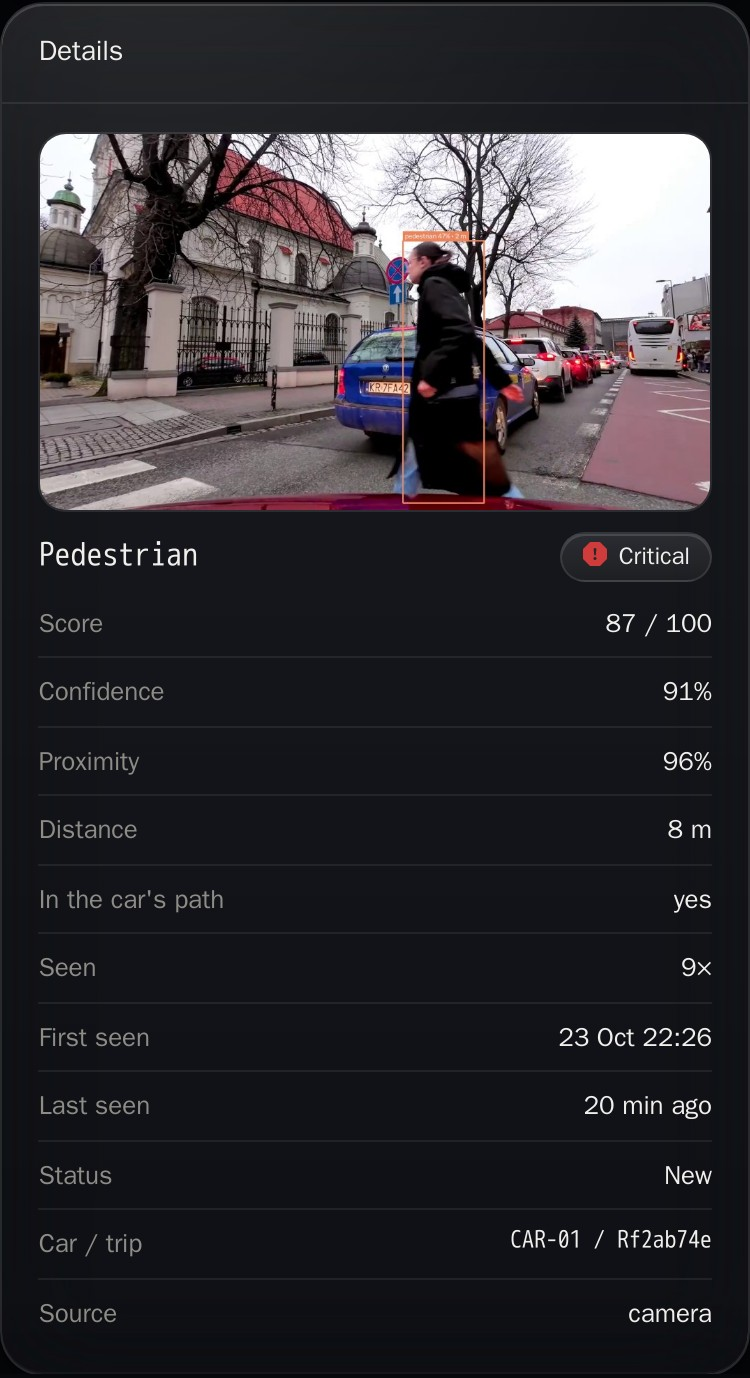
\includegraphics[width=\linewidth]{captures/obstacles_details_car01.jpg}
  \caption{Piéton sur la trajectoire : critique}
\end{subfigure}\hfill
\begin{subfigure}[b]{0.32\linewidth}\centering
  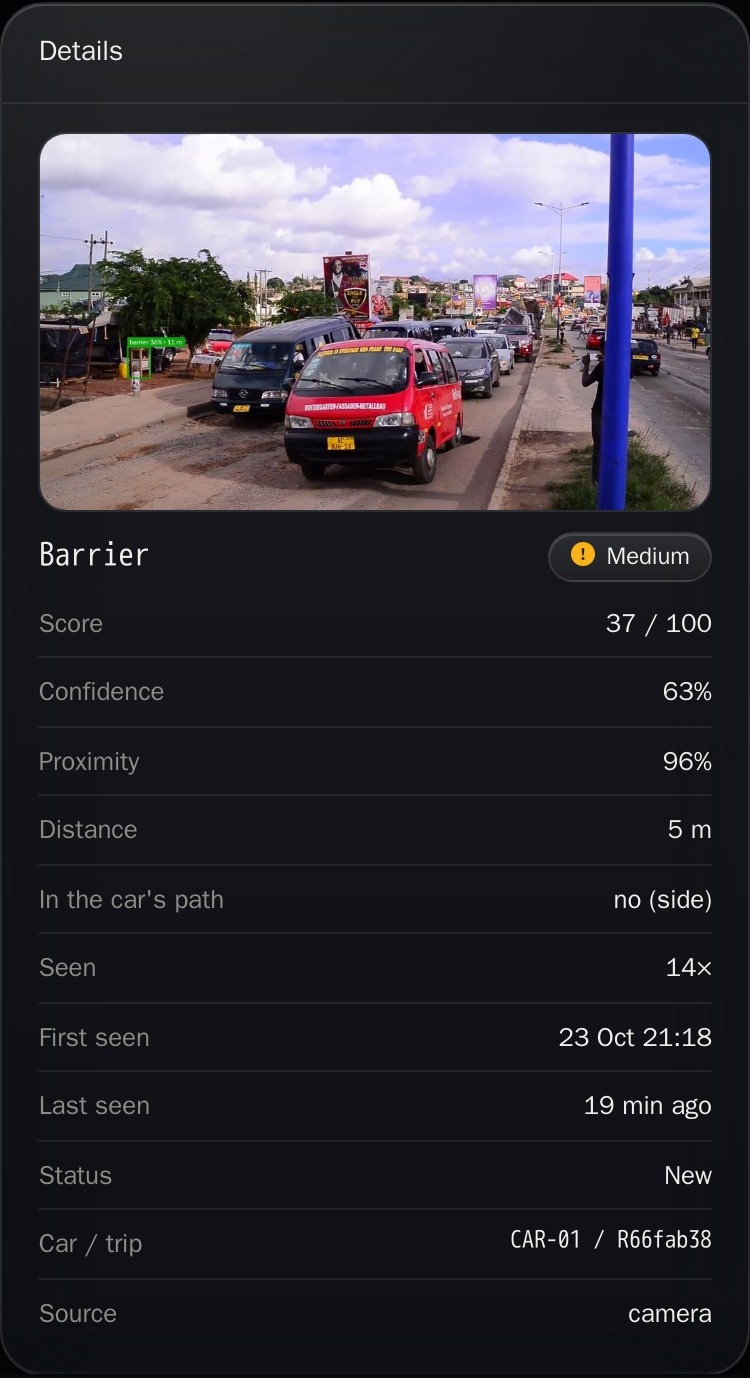
\includegraphics[width=\linewidth]{captures/obstacles_details_barrier.jpg}
  \caption{« Barrière » sur le côté : moyen}
\end{subfigure}\hfill
\begin{subfigure}[b]{0.32\linewidth}\centering
  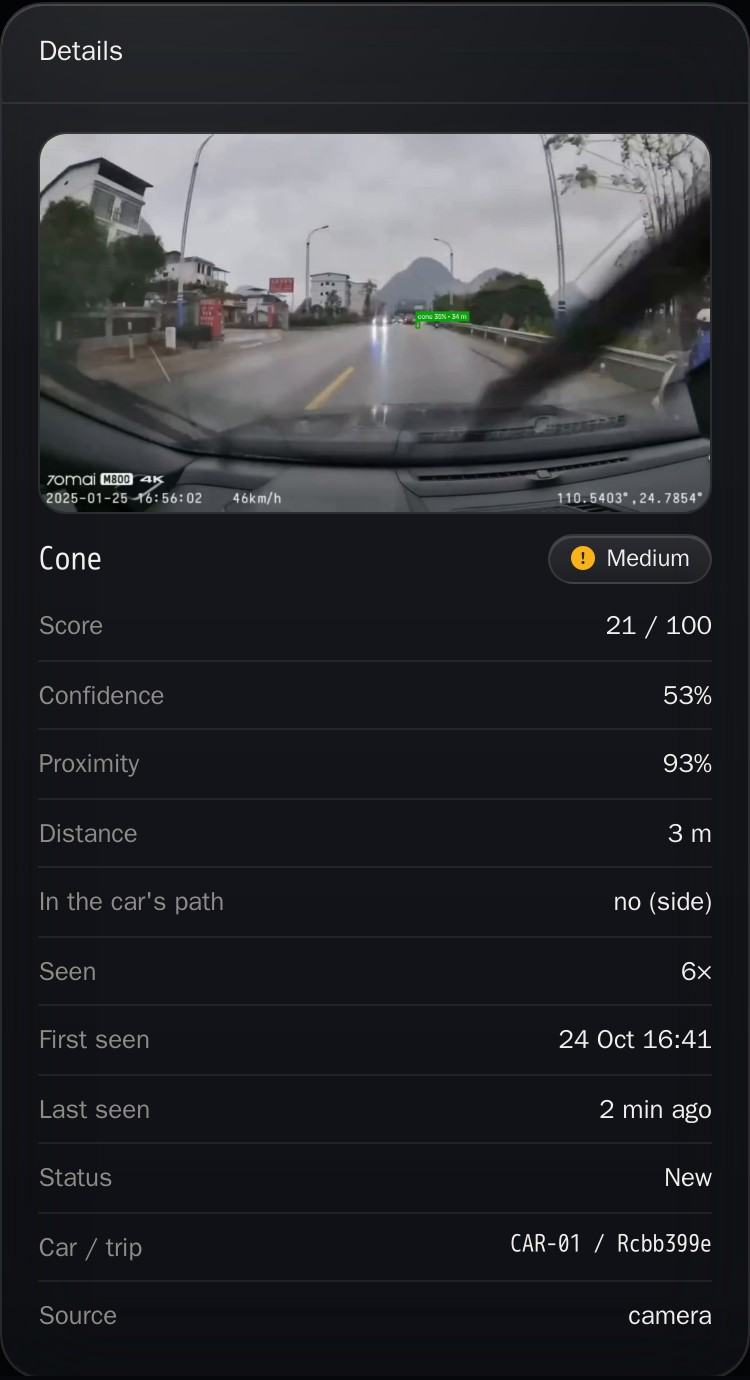
\includegraphics[width=\linewidth]{captures/obstacles_details_cone.jpg}
  \caption{Cône sur le côté : moyen}
\end{subfigure}

\vspace{0.2cm}
\begin{subfigure}[b]{\linewidth}\centering
  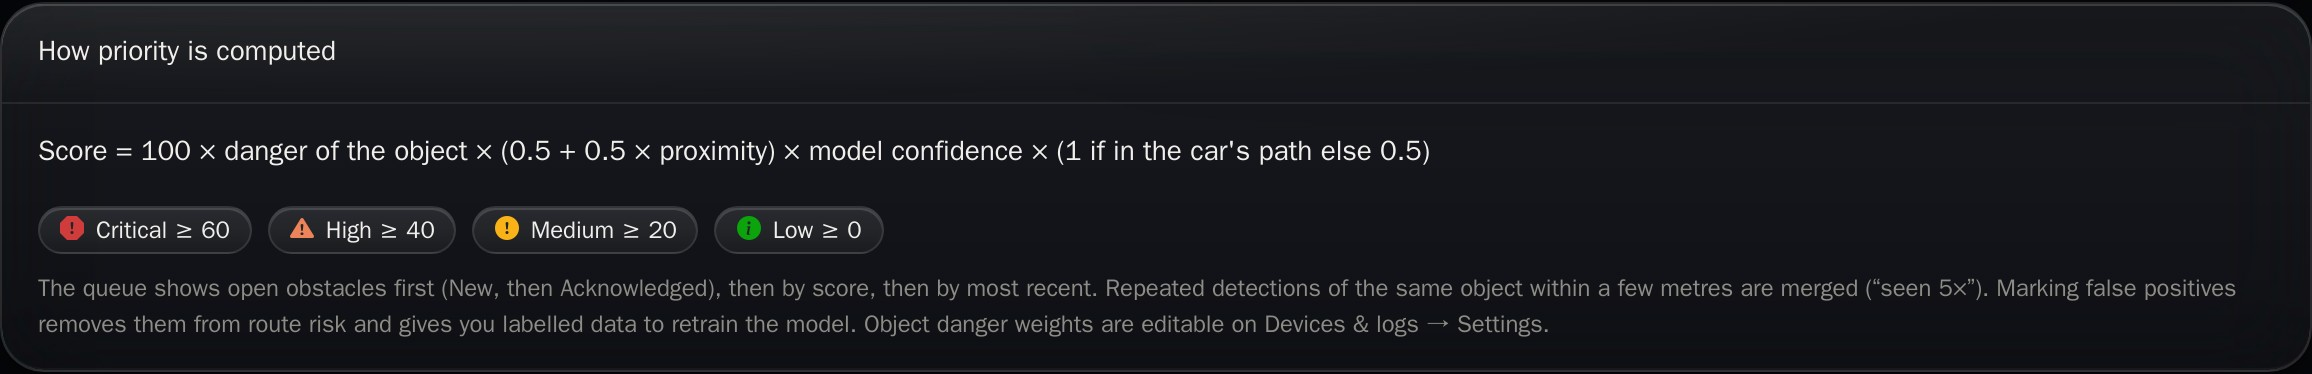
\includegraphics[width=\linewidth]{captures/obstacles_priority.jpg}
  \caption{Explication du calcul de la priorité}
\end{subfigure}
\caption{Niveaux de gravité et priorités : détail de trois obstacles détectés par la caméra embarquée}
\label{fig:obstacles-gravite}
\end{figure}

L'exemple de la « barrière » est instructif : l'instantané montre qu'il s'agit en réalité d'un poteau bleu. C'est
exactement le type d'erreur que l'opérateur peut signaler comme faux positif.

\subsection{Attribution des niveaux de priorité}
Le score détermine le niveau (critique, élevé, moyen, faible) et la file est triée par niveau puis par score. Les
indicateurs en tête de page comptent les obstacles ouverts de chaque niveau, le nombre d'obstacles revus et le taux de
faux positifs parmi eux (figure~\ref{fig:obstacles_kpis}). Les poids de danger étant réglables, l'opérateur peut
adapter la priorisation à son contexte ; tous les scores sont alors recalculés.

\capture{obstacles_kpis}{Indicateurs de la page Obstacles : obstacles ouverts par niveau, revues et faux positifs}

\subsection{Localisation et consultation des anomalies}
La sélection d'un obstacle affiche son détail : instantané annoté, classe et niveau, score, confiance, proximité,
distance, position par rapport à la trajectoire, nombre d'observations, dates, statut, véhicule, trajet et source.
La carte \emph{Where they are} situe tous les obstacles de la période. L'opérateur peut ensuite agir sur un ou
plusieurs obstacles sélectionnés : \textbf{Acknowledge} (pris en compte), \textbf{Resolve} (traité),
\textbf{False positive} (erreur du modèle) ou \textbf{Reopen}. Ces décisions modifient le risque utilisé par le
planificateur et alimentent l'évaluation des modèles.

\subsection{Filtrage et tri des obstacles}
La barre de filtres permet de choisir l'onglet (\emph{Needs review}, \emph{Acknowledged}, \emph{Closed},
\emph{All}), les niveaux affichés, les classes et la période (dernière heure, 24 heures, 7 jours, 30 jours, tout
l'historique) ; chaque colonne de la table peut être triée (figure~\ref{fig:obstacles_filters}).

\capture{obstacles_filters}{Barre de filtres de la page Obstacles}

% =================================================================================================
\section{Page Live Stats : statistiques et indicateurs}

La page \emph{Live stats} rassemble les indicateurs et graphiques statistiques (figure~\ref{fig:stats_real_ecran}).

\capture{stats_real_ecran}{Graphiques et indicateurs statistiques (monde réel)}

\subsection{Présentation des indicateurs statistiques}
En monde réel, les indicateurs sont : les véhicules en ligne, la distance parcourue et le nombre de trajets en
24 heures, la vitesse moyenne, le nombre moyen d'obstacles par heure, les manœuvres d'évitement et la batterie
moyenne. En prototype, ce sont l'état de la voiture, la source de données (caméra en direct ou démonstration), la
vitesse estimée, la cadence de la caméra, les parcours et les obstacles des dernières 24 heures
(figure~\ref{fig:stats-kpi}).

\begin{figure}[H]
\centering
\begin{subfigure}[b]{\linewidth}\centering
  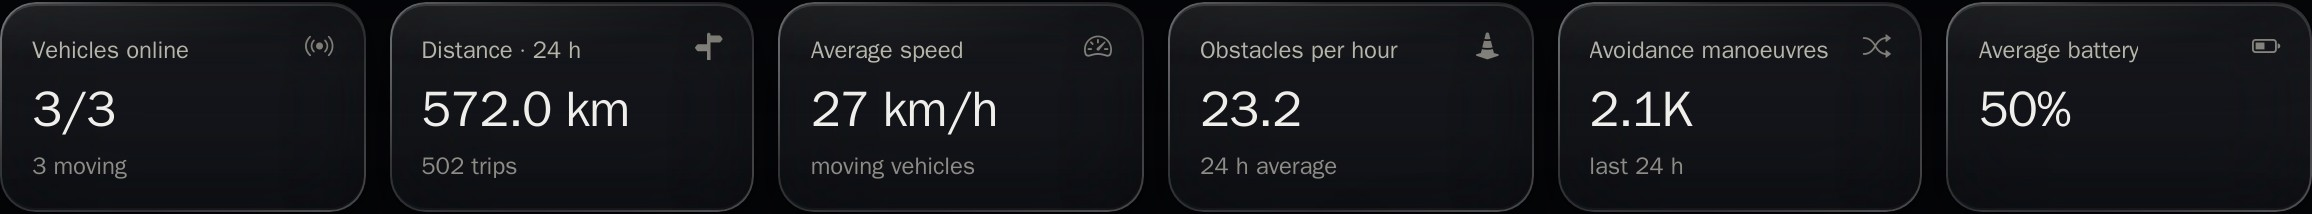
\includegraphics[width=\linewidth]{captures/stats_kpi_real.jpg}
  \caption{Monde réel}
\end{subfigure}

\vspace{0.2cm}
\begin{subfigure}[b]{\linewidth}\centering
  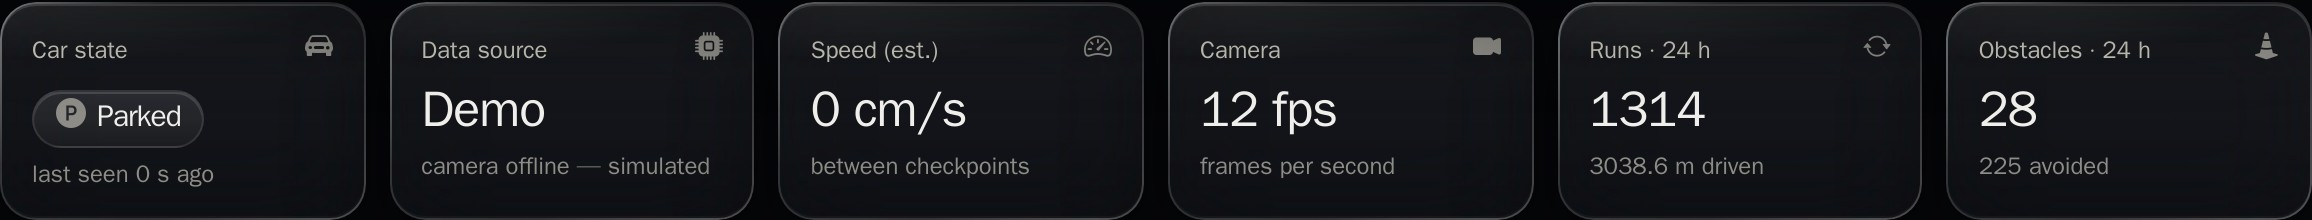
\includegraphics[width=\linewidth]{captures/stats_kpi_proto.jpg}
  \caption{Prototype}
\end{subfigure}
\caption{Indicateurs statistiques dans les deux environnements}
\label{fig:stats-kpi}
\end{figure}

\subsection{Nombre et répartition des obstacles détectés}
Le graphique \emph{Obstacles per hour} montre le nombre d'obstacles détectés par heure sur les dernières 24 heures,
ce qui fait apparaître les périodes chargées ; le graphique \emph{Obstacles by object} donne leur répartition par
classe sur 7 jours (figure~\ref{fig:stats-obstacles}).

\begin{figure}[H]
\centering
\begin{subfigure}[b]{0.49\linewidth}\centering
  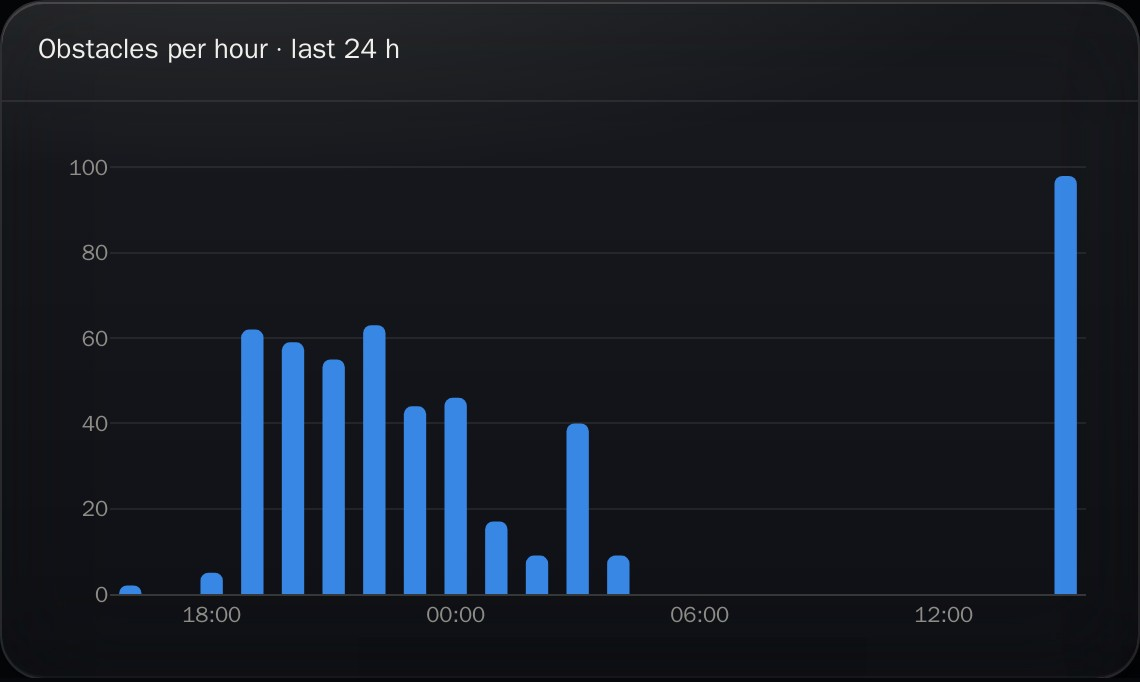
\includegraphics[width=\linewidth]{captures/stats_hourly.jpg}
  \caption{Obstacles par heure (24 h)}
\end{subfigure}\hfill
\begin{subfigure}[b]{0.49\linewidth}\centering
  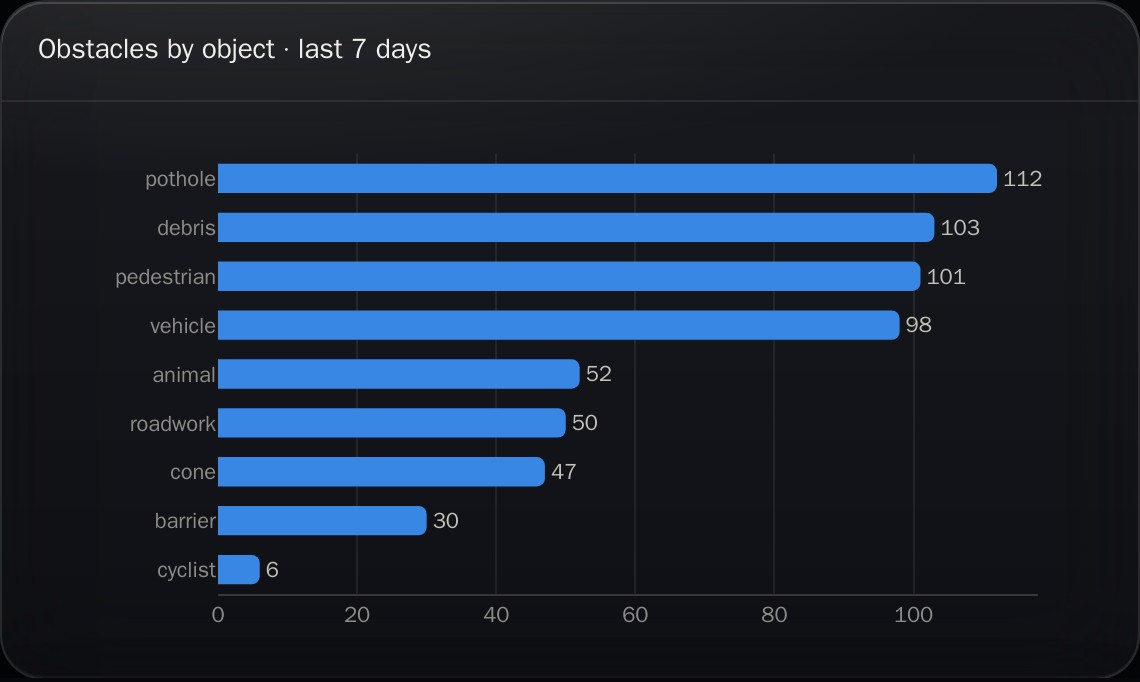
\includegraphics[width=\linewidth]{captures/stats_classes.jpg}
  \caption{Obstacles par classe (7 jours)}
\end{subfigure}
\caption{Nombre et répartition des obstacles détectés}
\label{fig:stats-obstacles}
\end{figure}

\subsection{Distribution des anomalies par gravité et priorité}
Le graphique \emph{Severity mix} montre, pour chaque jour, la part de chaque niveau de gravité parmi les obstacles
détectés (figure~\ref{fig:stats-severite}). Il permet de suivre l'évolution de la dangerosité et non seulement du
volume.

\subsection{Analyse des données de suivi des véhicules}
La chronologie \emph{Vehicle state} montre l'état de chaque véhicule (en route, en évitement, arrêté, en charge) sur
les 15 dernières minutes, le graphique \emph{Speed} leur vitesse sur 5 minutes, et le graphique des trajets par jour
l'activité de la flotte (figure~\ref{fig:stats-severite}).

\begin{figure}[H]
\centering
\begin{subfigure}[b]{0.49\linewidth}\centering
  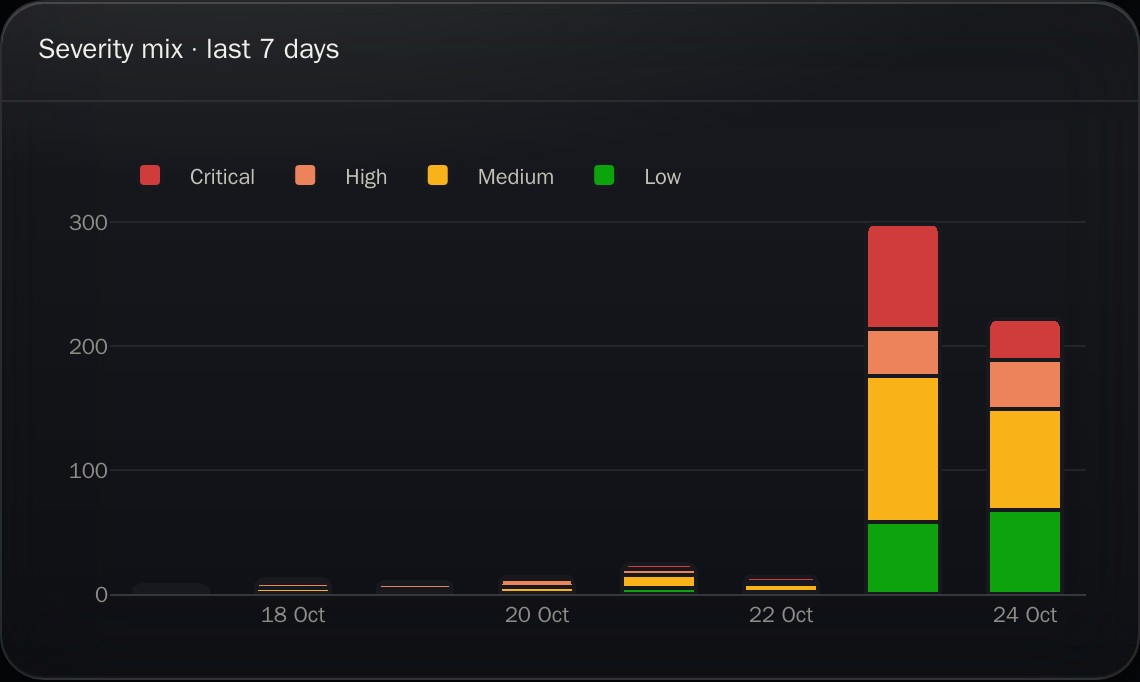
\includegraphics[width=\linewidth]{captures/stats_severity.jpg}
  \caption{Répartition par gravité}
\end{subfigure}\hfill
\begin{subfigure}[b]{0.49\linewidth}\centering
  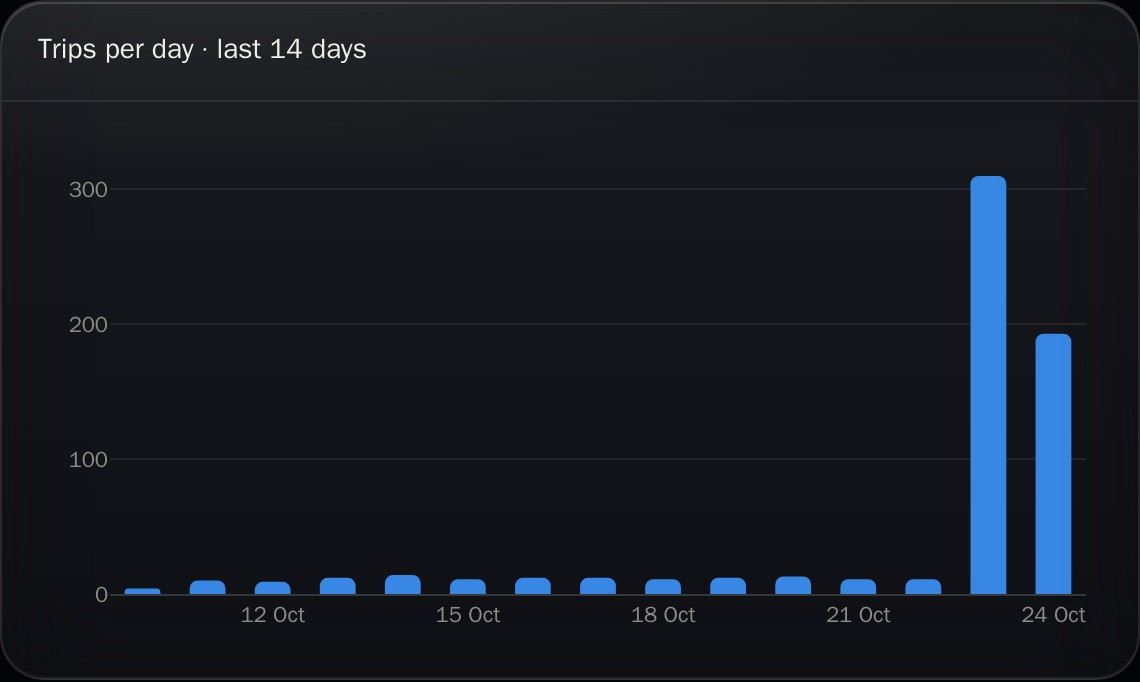
\includegraphics[width=\linewidth]{captures/stats_trips.jpg}
  \caption{Trajets par jour}
\end{subfigure}

\vspace{0.2cm}
\begin{subfigure}[b]{0.49\linewidth}\centering
  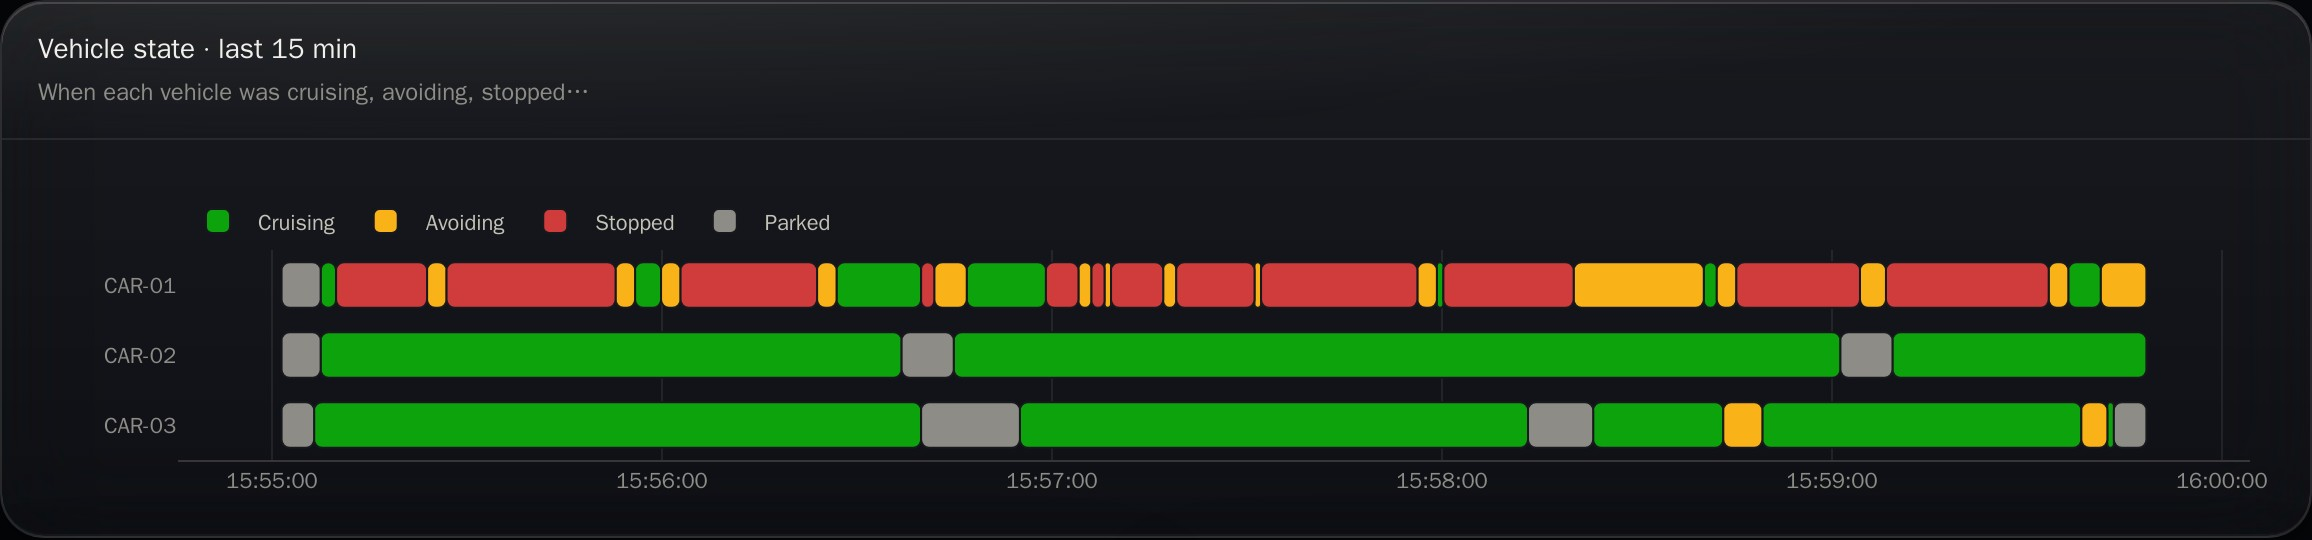
\includegraphics[width=\linewidth]{captures/stats_states.jpg}
  \caption{États des véhicules (15 min)}
\end{subfigure}\hfill
\begin{subfigure}[b]{0.49\linewidth}\centering
  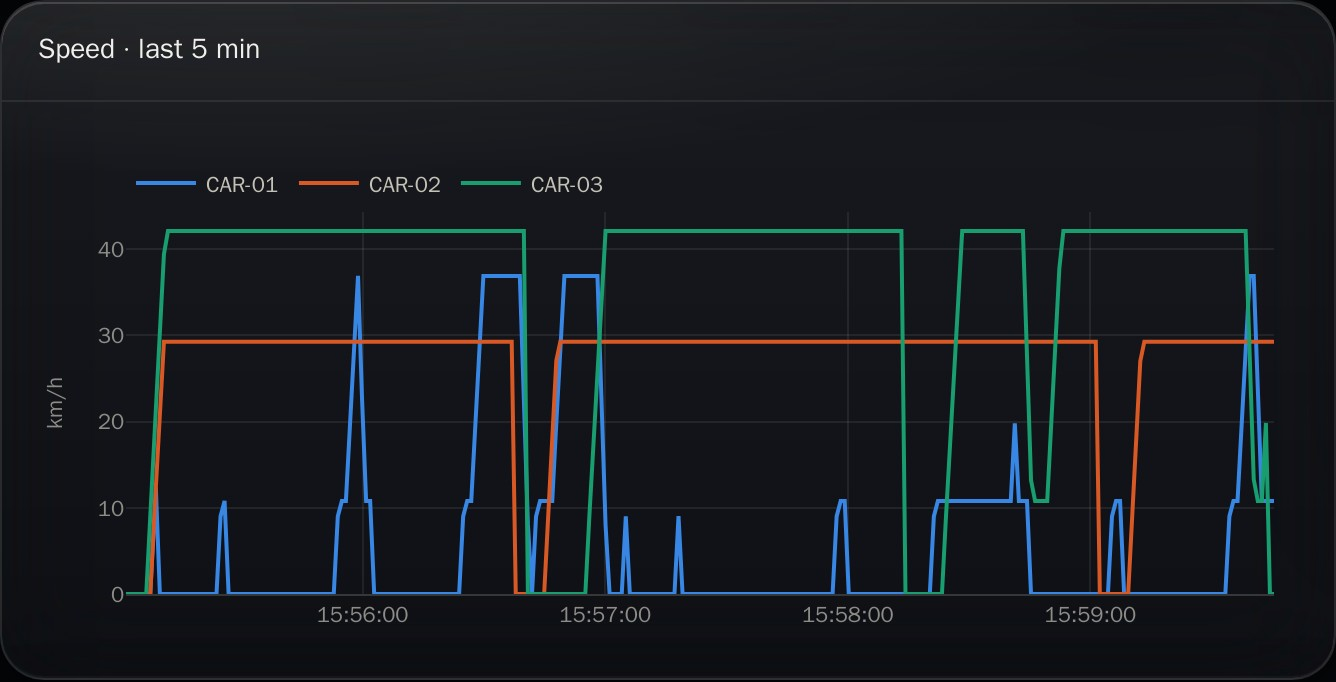
\includegraphics[width=\linewidth]{captures/stats_speed.jpg}
  \caption{Vitesse des véhicules (5 min)}
\end{subfigure}
\caption{Gravité des anomalies et données de suivi des véhicules}
\label{fig:stats-severite}
\end{figure}

\subsection{Visualisation graphique des statistiques}
Les graphiques sont construits avec Plotly et partagent une même charte : fond transparent sur les panneaux,
quadrillage discret, palette de couleurs catégorielles distinctes pour les séries, couleurs de gravité réservées aux
niveaux (rouge, orange, jaune, vert) et infobulles au survol. Les valeurs sont toujours accompagnées de leur unité.

\subsection{Comparaison des résultats entre les deux environnements}
Le changement d'environnement s'applique aussi aux statistiques : la même page présente les données de la flotte
simulée ou celles de la voiture du prototype (figure~\ref{fig:stats-env}). La comparaison doit tenir compte de la
nature des données : les statistiques du monde réel décrivent une flotte simulée dont seul CAR-01 voit de vraies
images, alors que celles du prototype décrivent des parcours réels sur la piste lorsque la caméra est connectée.

\begin{figure}[H]
\centering
\begin{subfigure}[b]{0.49\linewidth}\centering
  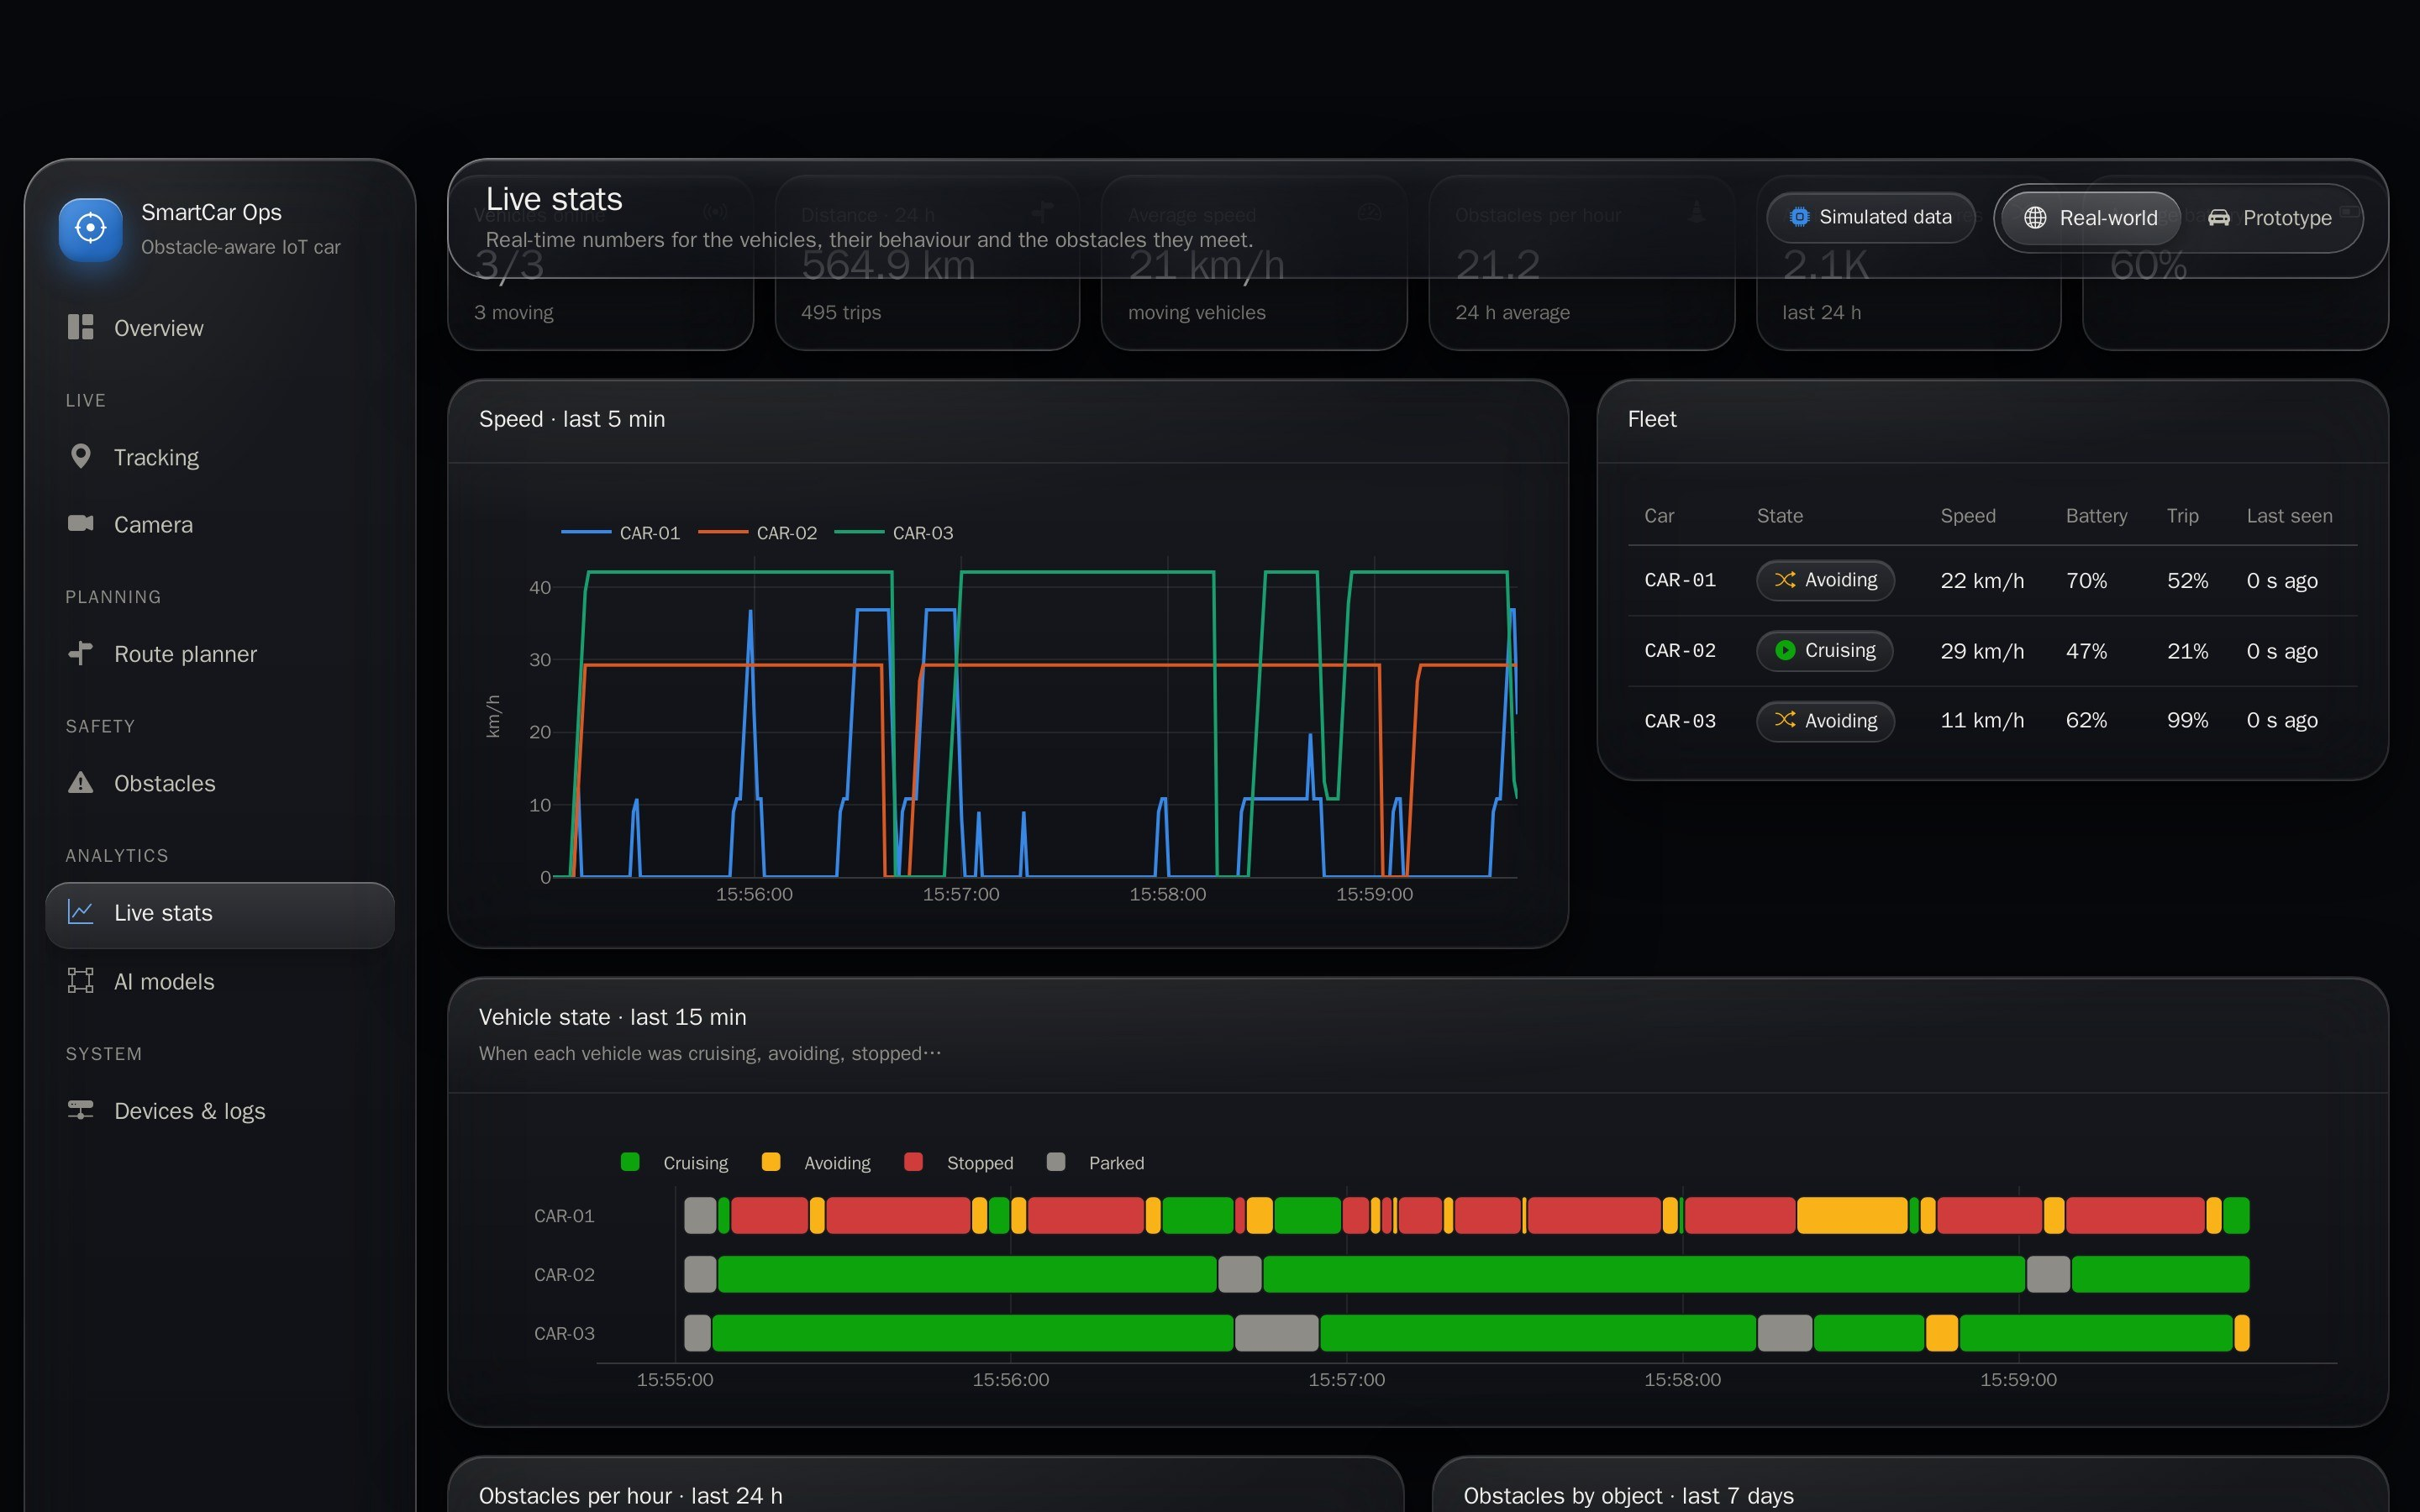
\includegraphics[width=\linewidth]{captures/stats_real_ecran.jpg}
  \caption{Monde réel}
\end{subfigure}\hfill
\begin{subfigure}[b]{0.49\linewidth}\centering
  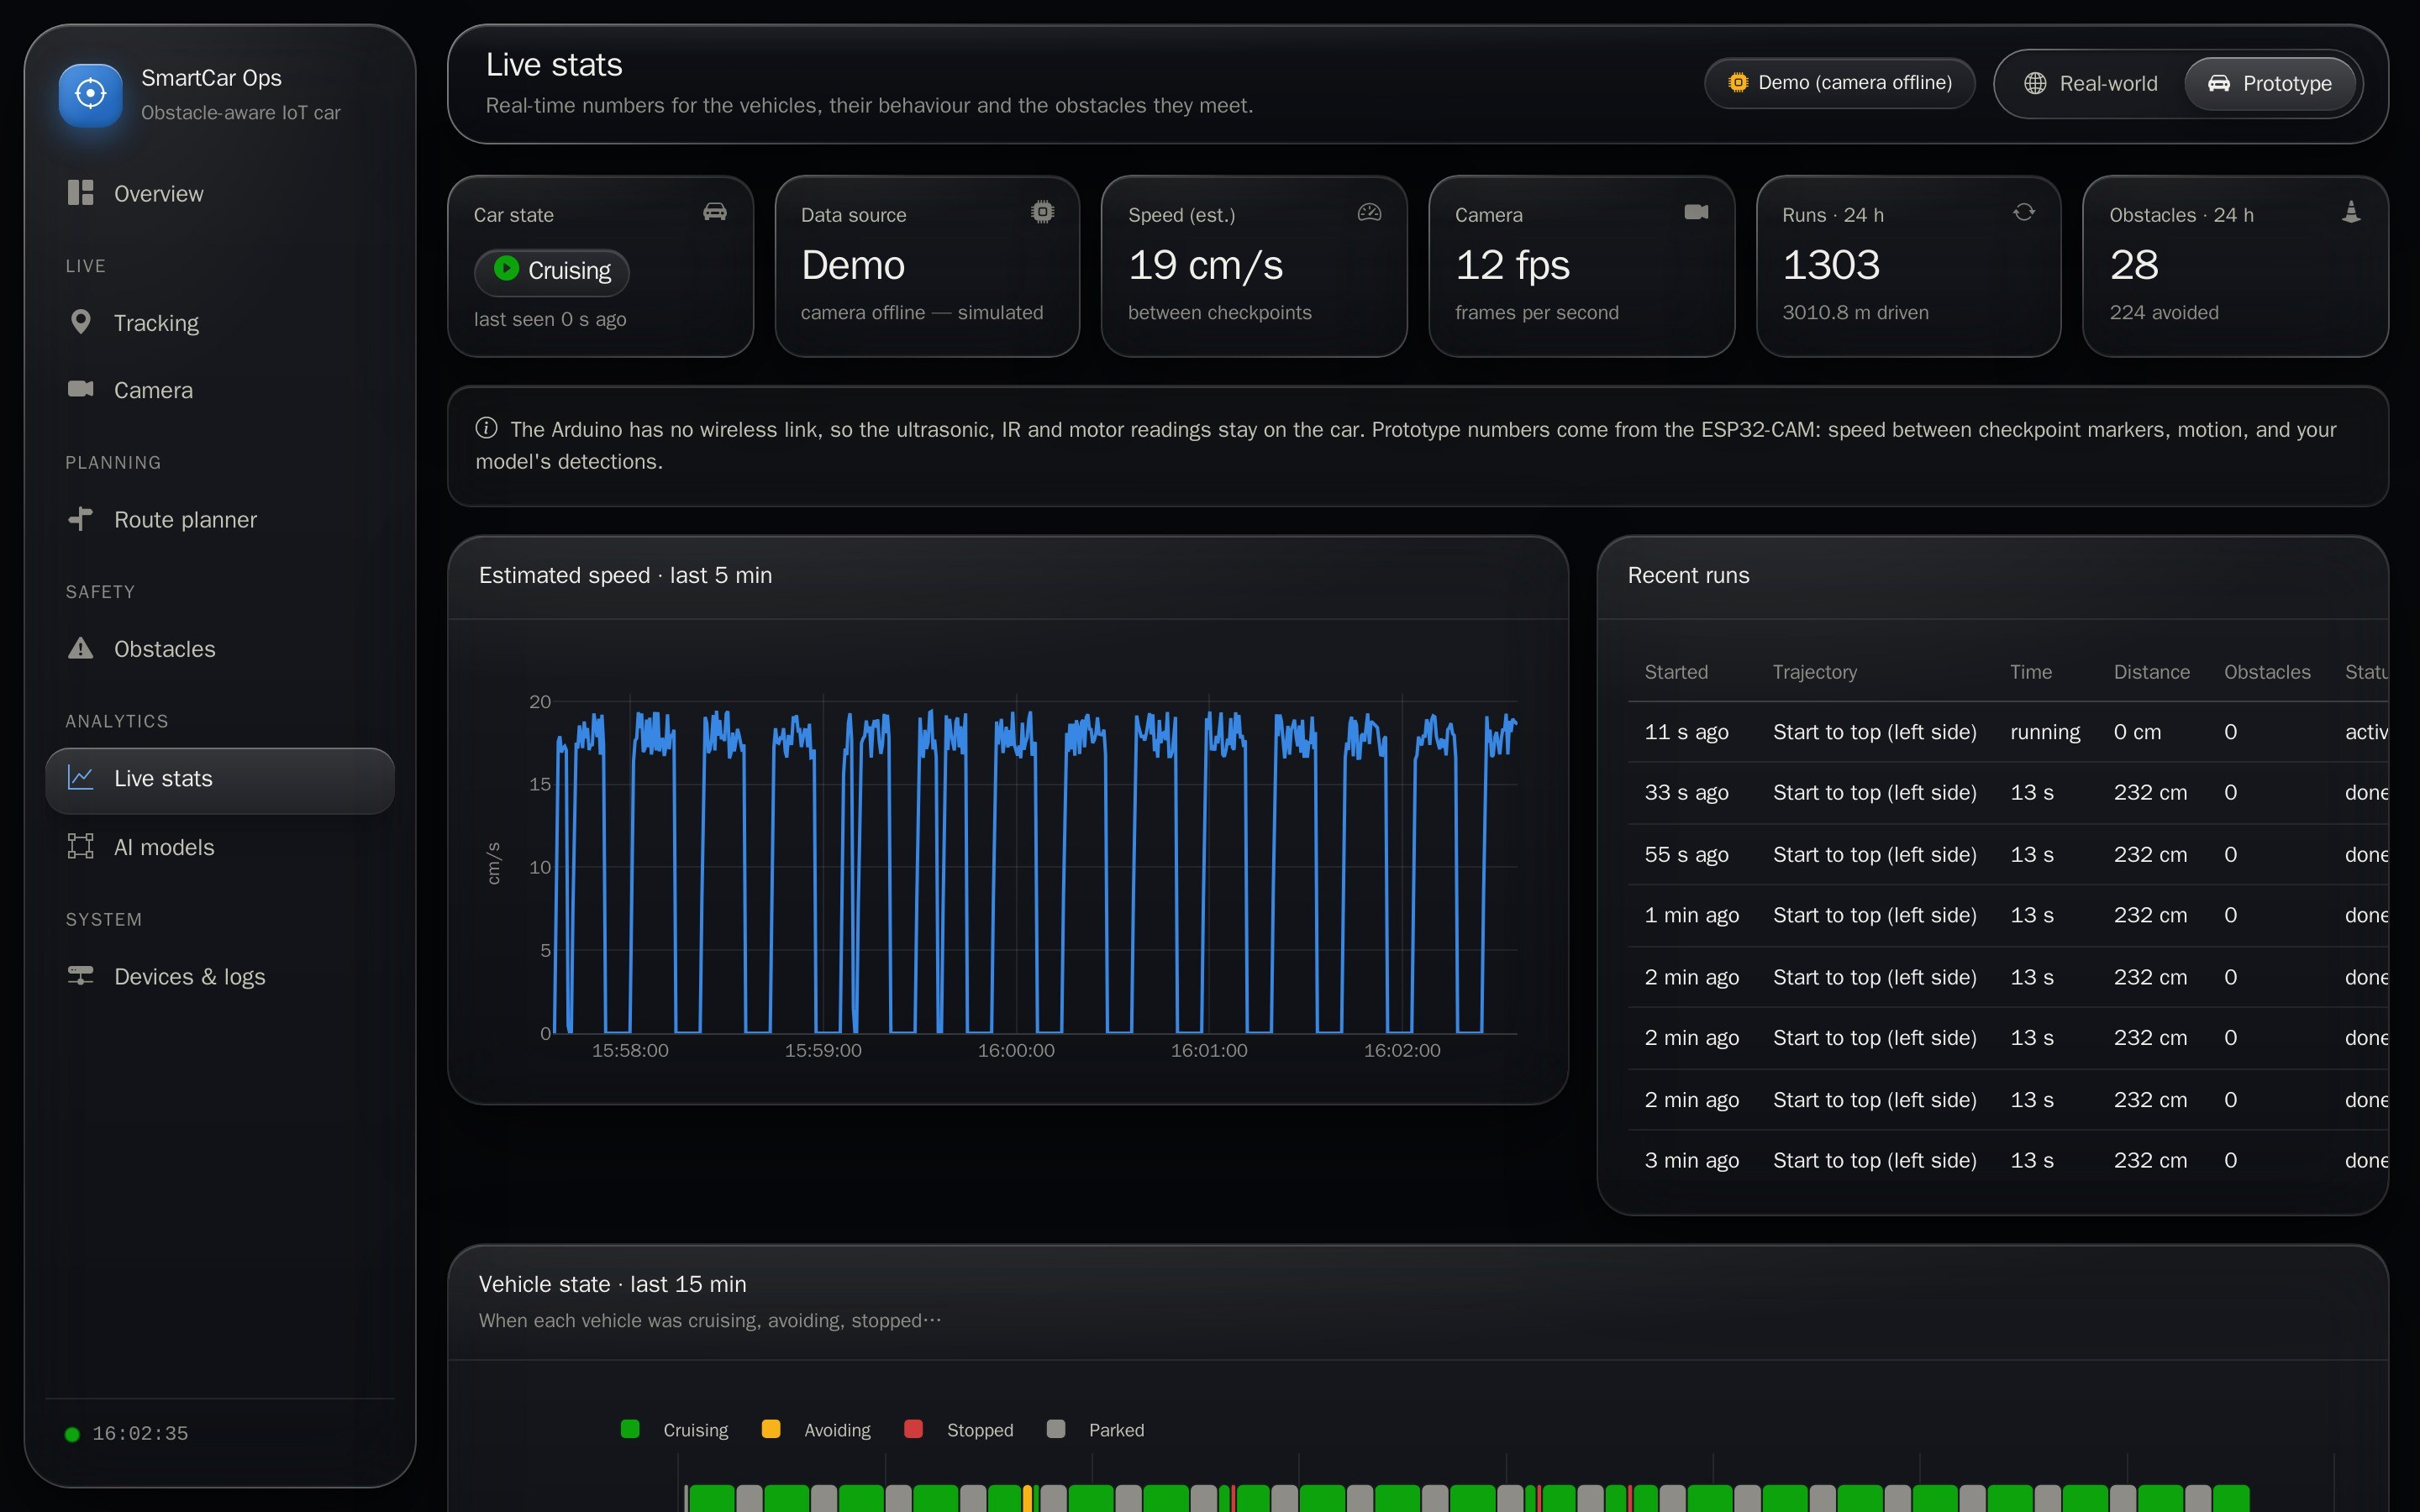
\includegraphics[width=\linewidth]{captures/stats_proto_ecran.jpg}
  \caption{Prototype}
\end{subfigure}
\caption{Page Live stats dans les deux environnements}
\label{fig:stats-env}
\end{figure}

% =================================================================================================
\section{Page AI Models : gestion des modèles d'intelligence artificielle}

La page \emph{AI models} présente, pour l'environnement choisi, chaque modèle avec son évaluation hors ligne, puis son
comportement sur la route (figure~\ref{fig:models_hazards}).

\capture{models_hazards}{Page de présentation des modèles : détecteur d'anomalies routières}

\subsection{Présentation des modèles utilisés}
Chaque modèle est présenté par une carte : nom, architecture, version, date d'entraînement, taille d'entrée, nombre
d'images, répartition entraînement / validation / test, durée d'entraînement et matériel, sources des données et
badge indiquant l'origine des métriques (évaluation sur un ensemble de test, modèle préentraîné, entraînement en
attente). Ces informations proviennent du registre \texttt{models/registry.json}, mis à jour par les notebooks
d'entraînement.

\subsection{Modèles YOLO26 pour les données réelles}
En monde réel, deux cartes sont affichées : le détecteur des usagers de la route (YOLO26n préentraîné sur COCO, avec
la liste des classes utilisées) et le détecteur d'anomalies routières (YOLO26s affiné). Pour ce dernier, deux
rangées de métriques sont présentées et clairement libellées : le meilleur réglage hors ligne (960 px avec TTA) et le
réglage temps réel utilisé dans l'application (640 px) (figure~\ref{fig:models_users}).

\capture[0.9]{models_users}{Carte du modèle des usagers de la route (préentraîné sur COCO)}

\subsection{Modèle YOLO26n pour le prototype}
En mode prototype, la carte du modèle des obstacles de la piste présente ses métriques sur les images de test
d'origine et sur leurs versions au style ESP32-CAM, la précision moyenne par classe et la matrice de confusion
(figure~\ref{fig:models_toy}).

\capture{models_toy}{Carte du modèle du prototype}

\subsection{Configuration et chargement des modèles}
La configuration est entièrement déclarative : chaque environnement dispose d'un profil qui liste ses modèles ONNX,
leur taille d'entrée, leur seuil de confiance et la correspondance de leurs classes. Un nouveau modèle se déploie en
copiant son fichier ONNX et en mettant à jour le profil, puis en redémarrant l'application ; un modèle manquant est
signalé sans bloquer le reste.

\subsection{Affichage des informations et des performances}
Les métriques hors ligne (précision, rappel, mAP@50, mAP@50-95, temps d'inférence sur GPU) sont complétées par deux
graphiques : la précision moyenne par classe et la matrice de confusion, normalisée par classe réelle et calculée au
seuil de confiance utilisé dans l'application. Le panneau \emph{On the road · last 7 days} mesure le comportement
réel : nombre de détections, confiance moyenne, nombre d'obstacles revus par l'opérateur, taux de faux positifs par
classe et modèle en cours d'utilisation (figure~\ref{fig:models_live}).

\capture{models_live}{Comportement des modèles sur la route (7 derniers jours)}

\subsection{Comparaison des résultats des modèles}
La page permet de confronter deux points de vue complémentaires : l'évaluation hors ligne, mesurée une fois sur un
ensemble de test annoté, et l'évaluation en service, construite progressivement à partir des revues de l'opérateur.
Un écart entre les deux (par exemple un taux de faux positifs élevé pour une classe) signale les classes à enrichir
lors du prochain entraînement ; les obstacles marqués comme faux positifs constituent alors des exemples
directement réutilisables.

% =================================================================================================
\section{Page Devices \& Logs : périphériques et journaux du système}

La page \emph{Devices \& logs} comporte trois onglets : \emph{Devices}, \emph{Event log} et \emph{Settings}
(figure~\ref{fig:system_devices_grid}).

\capture{system_devices_grid}{Périphériques et services du système}

\subsection{Présentation des périphériques connectés}
L'onglet \emph{Devices} présente une carte par équipement ou service : la caméra embarquée de CAR-01 (source, clip,
cadence vidéo et cadence d'analyse), l'ESP32-CAM (adresse IP, méthode de découverte, cadence, résolution, dernière
image), l'Arduino UNO (rappel de son rôle et de ses broches, sans liaison directe avec le serveur), les données du
prototype (piste, trajectoire active, points de passage), le simulateur du monde réel (véhicules, réseau routier), les
modèles chargés et la base de données (nombre de trajets, de points, d'obstacles et d'événements).

\subsection{Suivi de l'état des composants et des dispositifs}
Chaque carte porte un badge d'état (en ligne, hors ligne, en lecture, démonstration…) mis à jour en continu. Les
problèmes sont ainsi visibles immédiatement : une caméra introuvable, un modèle non chargé ou une source vidéo vide.

\subsection{Consultation des journaux d'exécution}
L'onglet \emph{Event log} affiche le journal des événements de l'environnement choisi : date, niveau (information,
avertissement, critique), catégorie et message. Il peut être filtré par niveau et par catégorie
(figure~\ref{fig:system_events_panel}).

\capture{system_events_panel}{Journal des événements}

\subsection{Gestion des événements et des erreurs}
Les événements sont enregistrés par tous les composants : début et fin de trajet, passage aux points de passage,
obstacle de niveau élevé ou critique, connexion et perte de la caméra, changement de statut d'obstacles, erreurs du
détecteur. Les erreurs ne bloquent pas l'application : une caméra perdue est recherchée à nouveau automatiquement, et
une erreur de modèle est signalée une seule fois dans le journal puis affichée sur la page Camera.

\subsection{Diagnostic et surveillance du système}
L'onglet \emph{Settings} permet de régler les poids de danger des classes, puis de recalculer tous les scores, et de
régénérer les données de démonstration (figure~\ref{fig:system_weights}). Associés à la page \emph{Camera} (état de la
connexion) et à la page \emph{AI models} (modèles chargés), ces outils permettent de diagnostiquer rapidement l'état du
système.

\capture[0.55]{system_weights}{Réglage des poids de danger des classes}

% =================================================================================================
\section{Synthèse des fonctionnalités de l'application}

\subsection{Interconnexion des différentes pages}
Les pages ne sont pas indépendantes : elles partagent les mêmes données et les actions faites sur l'une se
répercutent sur les autres (figure~\ref{fig:interactions}). Les détections de la page \emph{Camera} deviennent des
obstacles ; les décisions prises dans la page \emph{Obstacles} modifient le risque utilisé par le \emph{Route
planner} et alimentent le taux de faux positifs de la page \emph{AI models} ; les poids réglés dans \emph{Devices \&
logs} changent la priorité de tous les obstacles ; la trajectoire active choisie dans le planificateur sert à la
localisation de la voiture du prototype.

\begin{figure}[H]
\centering
\resizebox{0.95\linewidth}{!}{% Interactions entre les modules de l'application (chapitre 4)
\begin{tikzpicture}[
  p/.style={bloc,font=\footnotesize,minimum width=2.9cm,text width=2.7cm,minimum height=1.05cm,fill=bleufst!8},
  lb/.style={font=\scriptsize\itshape,text=encre!80,fill=white,inner sep=1pt,align=center}]
  \node[bloc,minimum width=3.8cm,text width=3.6cm,fill=gris!12,draw=gris,font=\footnotesize,minimum height=1.6cm] (core)
       at (0,0) {\textbf{Données partagées}\\hub en mémoire\\SQLite, réglages};
  \node[p] (ov)  at (0,4.0)    {Overview};
  \node[p] (tr)  at (-5.0,2.6) {Tracking};
  \node[p] (cam) at (-5.6,-0.6) {Camera};
  \node[p] (ob)  at (-3.4,-3.8) {Obstacles};
  \node[p] (pl)  at (3.4,-3.8) {Route planner};
  \node[p] (st)  at (5.0,2.6)  {Live stats};
  \node[p] (md)  at (5.6,-0.6)   {AI models};
  \node[p] (sys) at (0,-5.6)    {Devices \& logs};
  \foreach \n in {ov,tr,cam,ob,pl,st,md,sys} \draw[thick,draw=gris!70,dashed] (\n) -- (core);
  \draw[fleche] (cam) -- node[lb,left] {détections\\$\rightarrow$ obstacles} (ob);
  \draw[fleche] (ob) -- node[lb,below] {statut, gravité\\$\rightarrow$ risque des segments} (pl);
  \draw[fleche] ([yshift=0.25cm]ob.east) -- node[lb,pos=0.62,above,sloped] {revues $\rightarrow$ faux positifs} (md.south west);
  \draw[fleche] (sys) -- node[lb,left] {poids de danger\\$\rightarrow$ scores recalculés} (ob.south);
  \draw[fleche] ([yshift=0.3cm]pl.west) -- node[lb,pos=0.5,above,sloped] {trajectoire active (prototype)} (cam.south east);
  \draw[fleche] (tr) -- node[lb,above,sloped] {trajets} (ov);
  \draw[fleche] (ob.north) to[out=95,in=-120] node[lb,pos=0.85,left] {à traiter} (ov.south west);
  \draw[fleche] (cam.north) -- node[lb,left] {état du véhicule} (tr.south);
\end{tikzpicture}
}
\caption{Interactions entre les modules de l'application}
\label{fig:interactions}
\end{figure}

\subsection{Circulation des données entre les composants}
Les données suivent toujours le même chemin : acquisition par les services d'arrière-plan, analyse par les modèles,
enregistrement dans le hub et la base de données, lecture par les pages à chaque rafraîchissement, puis retour des
décisions de l'opérateur vers la base. Cette séparation entre acquisition et affichage garantit que l'interface reste
fluide quelle que soit la vitesse des modèles, et que plusieurs opérateurs peuvent consulter l'application en même
temps.

\subsection{Apports de l'application au système intelligent}
\app{} transforme les sorties brutes des modèles (des boîtes et des scores) en informations exploitables : des
obstacles localisés, dédupliqués, hiérarchisés et suivis dans le temps, intégrés à la planification des itinéraires.
Elle ferme la boucle entre la perception et la décision, et entre l'opérateur et les modèles, puisque ses revues
préparent les prochains entraînements. Enfin, en gérant les deux environnements avec la même chaîne logicielle, elle
montre que la solution validée sur le prototype est transposable à des données routières réelles.

\chapconclusion
Ce chapitre a présenté l'application \app : ses choix technologiques (Dash, Plotly, Docker), son architecture en
couches, la gestion de ses données et ses huit pages. L'application exécute les modèles en temps réel, priorise les
obstacles selon un score explicable, en tient compte dans la planification des itinéraires et permet à l'opérateur de
superviser aussi bien une flotte sur des routes réelles que la voiture du prototype.

\chapter*{Conclusion et perspectives}
\addcontentsline{toc}{chapter}{Conclusion et perspectives}
\markboth{Conclusion et perspectives}{}

Ce projet avait pour objectif de concevoir, avec des composants à faible coût, un système IoT capable de détecter les
obstacles sur le trajet d'un véhicule, d'en évaluer la gravité et d'exploiter ces informations en temps réel ; au terme
de ce travail, une chaîne complète a été réalisée, du capteur jusqu'à la décision. Sur le plan matériel, nous avons
construit une voiture miniature autour d'une carte Arduino UNO, d'un pont en H L298N, de deux moteurs à courant
continu, de deux capteurs infrarouges et d'un capteur ultrasonique, qui suit de façon autonome une piste tracée au
ruban adhésif et s'arrête devant un obstacle, tandis qu'une caméra ESP32-CAM diffuse en Wi-Fi les images prises de son
point de vue. Sur le plan de l'intelligence artificielle, nous avons entraîné des détecteurs YOLO26 dans un
environnement Docker reproductible : le détecteur d'anomalies routières, affiné pendant huit heures sur 7\,894 images
réelles, atteint un mAP@50 de 0,53 en temps réel (0,57 au meilleur réglage) sur des lieux absents de l'entraînement,
et le modèle du prototype, entraîné sur notre propre jeu de données annoté automatiquement avec SAM~2, reconnaît tous
les obstacles de son ensemble de test et détecte la boîte sur le flux réel de la caméra avec une confiance de
95\,\%. Sur le plan logiciel, l'application \app, développée avec Dash et Plotly, exécute ces modèles en temps réel,
transforme leurs détections en obstacles localisés et priorisés selon un score explicable, les intègre à la
planification des itinéraires et permet de superviser avec la même chaîne logicielle une flotte sur le réseau routier
réel d'un quartier de Paris et la voiture du prototype. Ce projet nous a permis de mettre en pratique l'ensemble des
notions du module (capteurs et actionneurs, microcontrôleurs, communication sans fil, traitement des données,
intelligence artificielle et supervision) et d'apprendre à évaluer honnêtement un modèle en identifiant ses limites.
Plusieurs perspectives permettraient de prolonger ce travail : enrichir les données du prototype avec des images
enregistrées par l'ESP32-CAM elle-même, dans différents lieux et éclairages, pour supprimer les fausses détections sur
des objets inconnus ; améliorer le modèle routier par un entraînement plus long et davantage d'exemples de
nids-de-poule ; relier l'Arduino au système pour transmettre la distance ultrasonique et recevoir des consignes du
serveur ; localiser précisément la voiture grâce aux marqueurs ArUco sur la piste et, dans le monde réel, à un module
GPS ; exécuter les modèles sur un calculateur embarqué (Raspberry Pi, Jetson) pour réduire la latence ; et enfin
déployer l'application sur un serveur accessible à distance, avec des notifications en cas d'obstacle critique.


\cleardoublepage
\phantomsection
\addcontentsline{toc}{chapter}{Bibliographie}
\printbibliography[title={Bibliographie}]

\end{document}
